%%%%%%%%%%%%%%%%%%%%%%%%%%%%%%%%%%%%%%%%%%%%%%%%%%%%%%%%%%%%%%%%%%%%%
%%                                                                 %%
%% Please do not use \input{...} to include other tex files.       %%
%% Submit your LaTeX manuscript as one .tex document.              %%
%%                                                                 %%
%% All additional figures and files should be attached             %%
%% separately and not embedded in the \TeX\ document itself.       %%
%%                                                                 %%
%%%%%%%%%%%%%%%%%%%%%%%%%%%%%%%%%%%%%%%%%%%%%%%%%%%%%%%%%%%%%%%%%%%%%

\documentclass[pdflatex,sn-mathphys]{sn-jnl}% Basic Springer Nature Reference Style/Chemistry Reference Style

%%%% Standard Packages and macros (don't forget to paste the macros in
%%%% the main at the end of the writing).
\usepackage{todonotes}
\usepackage{lstvhdl, lstautogobble, lstpseudocoq, lstcoq}
\usepackage{enumitem}
\usepackage{ebproof}
\ebproofset{left label template=\fontsize{9}{11}\selectfont\inserttext}
\ebproofset{right label template=\fontsize{7}{10}\selectfont\inserttext}

%%%%%%%%%%%%%%%%%%%%%%%%%%%%%%%%%%%%%%
%%%%%%% Misc. macros and defs. %%%%%%%
%%%%%%%%%%%%%%%%%%%%%%%%%%%%%%%%%%%%%%

% Macro definitions.

\def\bbook{\textsf{B}-Book}
\def\bmth{\textsf{B}}
\def\cakeml{\textsf{CakeML}}
\def\cnrs{\textsf{CNRS}}
\def\coq{\textsf{Coq}}
\def\java{\textsf{Java}}
\def\hilecop{\textsf{HILECOP}}
\def\inria{\textsf{Inria}}
\def\isahol{\textsf{Isabelle/HOL}}
\def\isa{\textsf{Isabelle}}
\def\hol{\textsf{HOL}}
\def\ccert{\textsf{CompCert}}
\def\lirmm{\textsf{LIRMM}}
\def\lustre{\textsf{Lustre}}
\def\nasa{\textsf{NASA}}
\def\um{\textsf{Universit\'e de Montpellier}}
\def\neurin{\textsf{NEURINNOV}}
\def\uml{\textsf{UML}}
\def\vhdl{\textsf{VHDL}}
\def\hvhdl{$\mathcal{H}$-\textsf{VHDL}}
\def\lwidth{\dimexpr\linewidth-2\fboxsep-2\fboxrule}
\def\ocaml{\textsf{OCaml}}

%%% Local Variables:
%%% mode: latex
%%% TeX-master: "main"
%%% End:


%%%%

\jyear{2022}%

%% as per the requirement new theorem styles can be included as shown below
\theoremstyle{thmstyleone}%
\newtheorem{theorem}{Theorem}%  meant for continuous numbers
%%\newtheorem{theorem}{Theorem}[section]% meant for sectionwise numbers
%% optional argument [theorem] produces theorem numbering sequence instead of independent numbers for Proposition
\newtheorem{proposition}[theorem]{Proposition}% 
%%\newtheorem{proposition}{Proposition}% to get separate numbers for theorem and proposition etc.

\theoremstyle{thmstyletwo}%
\newtheorem{example}{Example}%
\newtheorem{remark}{Remark}%
\newtheorem*{pf}{Proof}%

\theoremstyle{thmstylethree}%
\newtheorem{definition}{Definition}%
\newtheorem{lemma}{Lemma}%

\raggedbottom
%%\unnumbered% uncomment this for unnumbered level heads

\begin{document}

\title[Formal verification of the \hilecop{} methodology]{Formal
  verification of a methodology for the design of safety-critical
  digital systems}

%%=============================================================%%
%% Prefix	-> \pfx{Dr}
%% GivenName	-> \fnm{Joergen W.}
%% Particle	-> \spfx{van der} -> surname prefix
%% FamilyName	-> \sur{Ploeg}
%% Suffix	-> \sfx{IV}
%% NatureName	-> \tanm{Poet Laureate} -> Title after name
%% Degrees	-> \dgr{MSc, PhD}
%% \author*[1,2]{\pfx{Dr} \fnm{Joergen W.} \spfx{van der} \sur{Ploeg} \sfx{IV} \tanm{Poet Laureate} 
%%                 \dgr{MSc, PhD}}\email{iauthor@gmail.com}
%%=============================================================%%

\author*[1]{\fnm{Vincent} \sur{Iampietro}}
\author[1]{\fnm{David} \sur{Delahaye}}
\author[1,2]{\fnm{David} \sur{Andreu}}

\email{Firstname.Lastname@lirmm.fr}
\email{David.Andreu@neurinnov.com}

\affil*[1]{\orgname{\lirmm, \um, \cnrs},
  \city{Montpellier}, \country{France}}

\affil[2]{\orgname{\neurin}, \city{Montpellier}, \country{France}}

\abstract{}

\keywords{}

\maketitle

\listoftodos

\section{Introduction}
\label{sec:intro}

The domain of Model-Based Systems Engineering (MBSE) \cite{Long2011}
proposes a framework to help engineers to design and produce digital
systems, in a well-documented, safe and reliable way. Comparable to
what Model Driven Engineering (MDE) does in the world of software
engineering, models are first order concepts in MBSE.  As illustrated
in Figure~\ref{fig:MBSE-ps}, a MBSE process describes a way to design
a digital system starting from a high-level specfication of the
system. This specification can follow a graphical formalism such as
SysML \cite{Friedenthal2014} or Petri nets (PNs) \cite{Petri1962}, or
a textual one such as SystemC \cite{Black2009} or VHDL
\cite{Ashenden2010}. Then, the MBSE process describes many refinement
phases (the downward-going green arrows in Figure~\ref{fig:MBSE-ps})
during which the input model will be transformed; at each refinement
phase, the model goes down in abstraction towards its final
implementation as a hardware circuit. A refinement phase, which is
also a transformation phase, can be performed automatically or
manually.

\begin{figure}[H] \centering
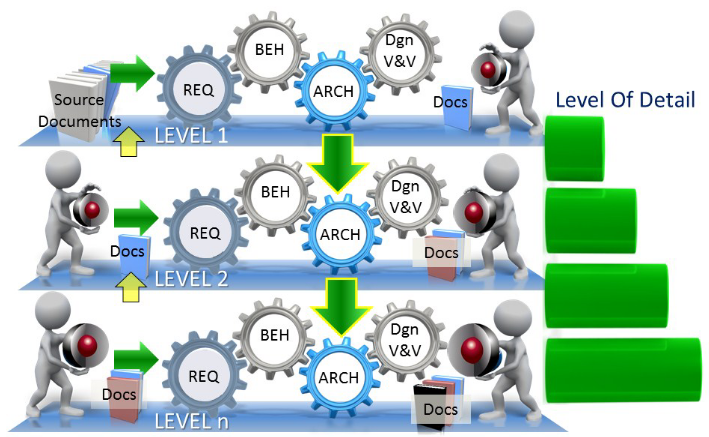
\includegraphics[keepaspectratio,width=.6\textwidth]{MBSE-ps.png}
  \caption[A Model-Based Systems Engineering process.]{A Model-Based
Systems Engineering process; REQ stands for requirements, BEH for
behavior, ARCH for architecture, Dgn V\&V for design verification and
validation. This figure is an excerpt from \cite{Long2011}.}
  \label{fig:MBSE-ps}
\end{figure}

In the case where the digital system being designed is a
safety-critical system, an MBSE process will often employ formal
models as the design formalism. Thus, these models enable a certain
extent of mathematical reasoning to prove that safety properties are
met during the design V\&V phase (cf. Figure~\ref{fig:MBSE-ps}).

To assist the engineers in the design and the implementation of
safety-critical digital systems, the CAMIN team came up with a process
called the ``\hilecop{} methodology'' \cite{Andreu2009}.  This
methodology follows the principles of a MBSE process and relies on
several transformations going from abstract models to concrete FPGA
(Field-Programmable Gate Array) or digital ASIC (Application-Specific
Integrated Circuit) implementations through the production of VHDL
code. Figure~\ref{fig:hilecop-wf} details the global workflow of
\hilecop{}.

\begin{figure}[H]
\centering
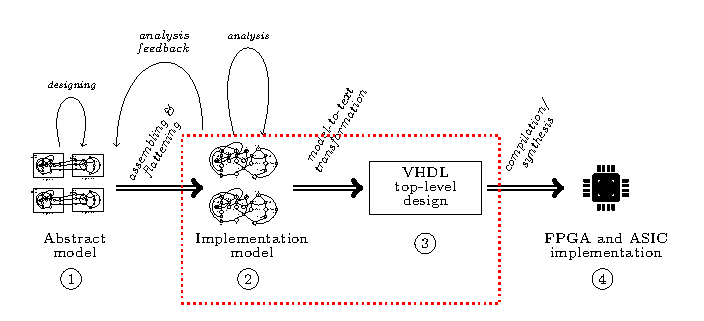
\includegraphics[keepaspectratio=true,width=\textwidth]{hilecop-wf.eps}
\caption[Workflow of the \hilecop{} methodology.]{Workflow of the
  \hilecop{} methodology; horizontal double arrows indicate the
  transformation phases, i.e. the refinement phases in MBSE terms;
  simple arrows indicate different kinds of operations performed at a
  given step.}
\label{fig:hilecop-wf}
\end{figure}

In Figure~\ref{fig:hilecop-wf}, Step~1 corresponds to the design phase
of a digital system. At this step, the user produces a model of the
required system; the leveraged model formalism is a graphical
formalism based on component diagrams and Petri nets (PNs).  In
Figure~\ref{fig:hilecop-wf}, the transformation from Step~1 to Step~2
flattens the model. The internal behaviors of separate components are
connected according to the interface compositions, and embedding
component structures are removed. The result of this transformation
step is a global PN that represents the behavior of the digital
system.  The class of PNs used in \hilecop{} has been specifically
devised for the design of safety-critical digital systems; a first
thesis has formalized the execution semantics of these PN models
\cite{Leroux2014}. % What makes them a very
% particular kind of models is their \textit{synchronous} execution
% semantics. This semantics denotes from the standard
% \textit{asynchronous} execution of PNs.
Due to its mathematical
foundations, a PN model can be analyzed, and a proof that a given
model meets some properties can be automatically produced through the
direct analysis of the structure or through the use of model-checking
techniques. This feature of PNs has been one of the reason of the
adoption of this formalism as \hilecop{}'s base formalism. A thesis
has been dedicated to the development of new methods to analyze the
\hilecop{} PN models \cite{Merzoug2018}. The analysis phase is here to
convince the engineers that they are indeed designing a safe
system. The analysis process is a round trip between Step~1 and
Step~2.  It aims at producing a model that is conflict-free (see
Section~\ref{sec:hilecop-models} for more details about the definition
of a conflict), bounded, and deadlock-free, using model-checking
techniques.  After several iterations, the model should reach
soundness and is then said to be \emph{implementation-ready}.

In Figure~\ref{fig:hilecop-wf}, from Step~2 to Step~3, \vhdl{} source
code is then generated by means of an automatic model-to-text
transformation. The generated code describes a \vhdl{} design, i.e. a
textual description of a hardware system, which has an interface
defining input and output ports and an internal behavior called an
architecture.

From Step~3 to Step~4, the \vhdl{} compilation/synthesis and the FPGA
programming, or ASIC realization, are finally performed using
industrial tools. At the end of Step~4, the designed circuit is
physically built on an FPGA device or an ASIC.  What happens between
Step~3 and Step~4 appears as a black box in the whole \hilecop{}
methodology. Therefore, we will not consider this circuit synthesis
phase in our verification process.

% \subsection{Verifying the \hilecop{} methodology}
% \label{sec:verif-hilecop}

The use of Petri nets as a base model is one of the major advantage of
the \hilecop{} methodology. All the analysis tools that accompany the
Petri net formalism, and allow us to prove that the models meet some
required properties, qualify the \hilecop{} methodology as a formal
method for the design and implementation of safety-critical digital
systems. However, the advantages provided by the use Petri nets would
be lost if one of the transformations performed during the process
changes the input model in a way that would alter its behavior. % Thus,
% the engineers would have specified a perfectly correct digital
% system but would never obtain the expected circuit on a physical
% device.
In order to reinforce the confidence in the \hilecop{} methodology,
the goal of our work is to verify, by establishing a formal proof,
that the model-to-text transformation from Step~2 to Step~3, referred
to as the HM2T, preserves the behavior of the input models into the
generated \vhdl{} designs. We choose to carry out this task as a
deductive verification task.  We aim at proving a that the HM2T is
\textit{semantic-preserving}. According to the literature
\cite{Patrignani2019,Leroy2009}, this is expressed through a
\textit{correctness} theorem of the following form: a given
transformation function is semantic-preserving if for any source
instance (i.e. a program, a model, etc.) passed as input the resulting
output instance has the same behavior as the source at runtime.  In
the case of the HM2T, the theorem is of the following form: for all PN
model, input to the transformation, the generated output \vhdl{}
design behaves similarly at runtime. The proof will be mechanized with
the \coq{} proof assistant.

The task of formally verifying the \hilecop{} model-to-text
transformation can appear as yet another proof of semantic
preservation for yet another transformation function. Proving a
semantic preservation theorem for a transformation program, and
implementing the proof within a proof assistant, is now a well-known
task and many successful works can be found in the literature
(cf. Section~\ref{sec:related-work}).  Therefore, the scientific
interest of our research comes from the specificities of the HM2T
compared to the other transformations that have been formally
verified. Mostly, in the literature, the transformation programs that
are formally verified are compilers for programming languages. From
this fact naturally arises the will to compare the HM2T to a compiler
program, and to determine which elements could introduce additional
technical difficulties regarding the formal verification process.  To
begin with, the input formalism of the HM2T depends on Petri nets,
which are quite abstract mathematical models, and thus is not a common
programming language.  Moreover, the output language, \vhdl{}, is also
not a common programming language as its purpose is both the
structural and behavioral description of hardware circuits. By their
very nature, all instructions defining the behavior of circuits in
\vhdl{} have a concurrent execution logic. This also differs from the
execution of programs written in generic programming languages which
are often sequential programs.

% To further motivate the necessity of the verification task, the
% development of neuroprostheses by the INRIA CAMIN team is at the base
% of the creation of the Neurrinov
% company\footnote{\url{http://neurinnov.com/}}. The Neurrinov company
% is now looking towards the industrial development of such
% neuroprostheses. We hope that once the verification performed on the
% \hilecop{} methodology, it will help to obtain the CE certification,
% related to the EU 2017/745 regulation text, necessary to qualify the
% neuroprostheses as eligible for the medical market.

Moreover, the \hilecop{} methodology comes with a working
implementation based on the Eclipse framework used by the CAMIN team
to design and develop neuroprostheses. % This software is currently used
% by the engineers of the Neurinnov company to design the digital
% systems having a part in safety-critical implantable medical devices.
To the purpose of formal verification, we will implement the
\hilecop{} model-to-text transformation leveraging the functional
language of the \coq{} proof assistant. However, after the
mechanization of the proof of semantic preservation, we could use the
extraction feature of the \coq{} proof assistant to produce the
implemented transformation as an \ocaml{} program. Then, we will be
able to connect this program to the existing \hilecop{} software in
order
to use the verified version of the transformation.\\

This article is structured as
follows. Section~\ref{sec:hilecop-models} presents the specific kind
of Petri net models that are the input of \hilecop{}'s model-to-text
transformation along with their formal semantics.
Section~\ref{sec:hvhdl} gives a formal definition of the syntax and
semantics of a subset of the \vhdl{} language that we call
\hvhdl{}. \hvhdl{} is the target language of the programs generated by
\hilecop{}'s model-to-text transformation.  Section~\ref{sec:m2t}
presents the transformation through its formal specification.
Section~\ref{sec:proof} details the semantic preservation theorem
expressing that the \hilecop{} transformation is semantic-preserving.
It also gives the high-level theorems and lemmas involved in the proof
of the semantic preservation theorem.  Finally,
Section~\ref{sec:concl} ends the article, and outlines the
perspectives regarding the full verification of the \hilecop{}
methodology.

\section{Models of digital systems in \hilecop{}}
\label{sec:hilecop-models}

Let us introduce the input formalism of \hilecop{}'s model-to-text
transformation: Synchronously executed, extended, generalized,
Interpreted Time Petri Nets with priorities (SITPNs). The
formalization of the SITPN structure and semantics is mainly the
result of two Ph.D. theses \cite{Leroux2014,Merzoug2018}. We made a
preciser definition of both the SITPN structure and its semantics, as
precision is needed for proving semantic preservation. We have
implemented both structure and semantics in
\coq{}\footnote{\url{https://github.com/viampietro/ver-hilecop/tree/master/sitpn}}. Moreover,
we added complementary definitions, concerning the well-definition of
an SITPN input model, that are required to express our semantic
preservation theorem. In this section, we assume that the reader has
some knowledge of the Petri net formalism and its semantics, so that
words like firing, or marking, need no explanation. For more
information on the topic of Petri nets, the reader can refer to
\cite{David1994}, \cite{Murata1989}, or \cite{Diaz2001}.

\begin{figure}[H]
\centering
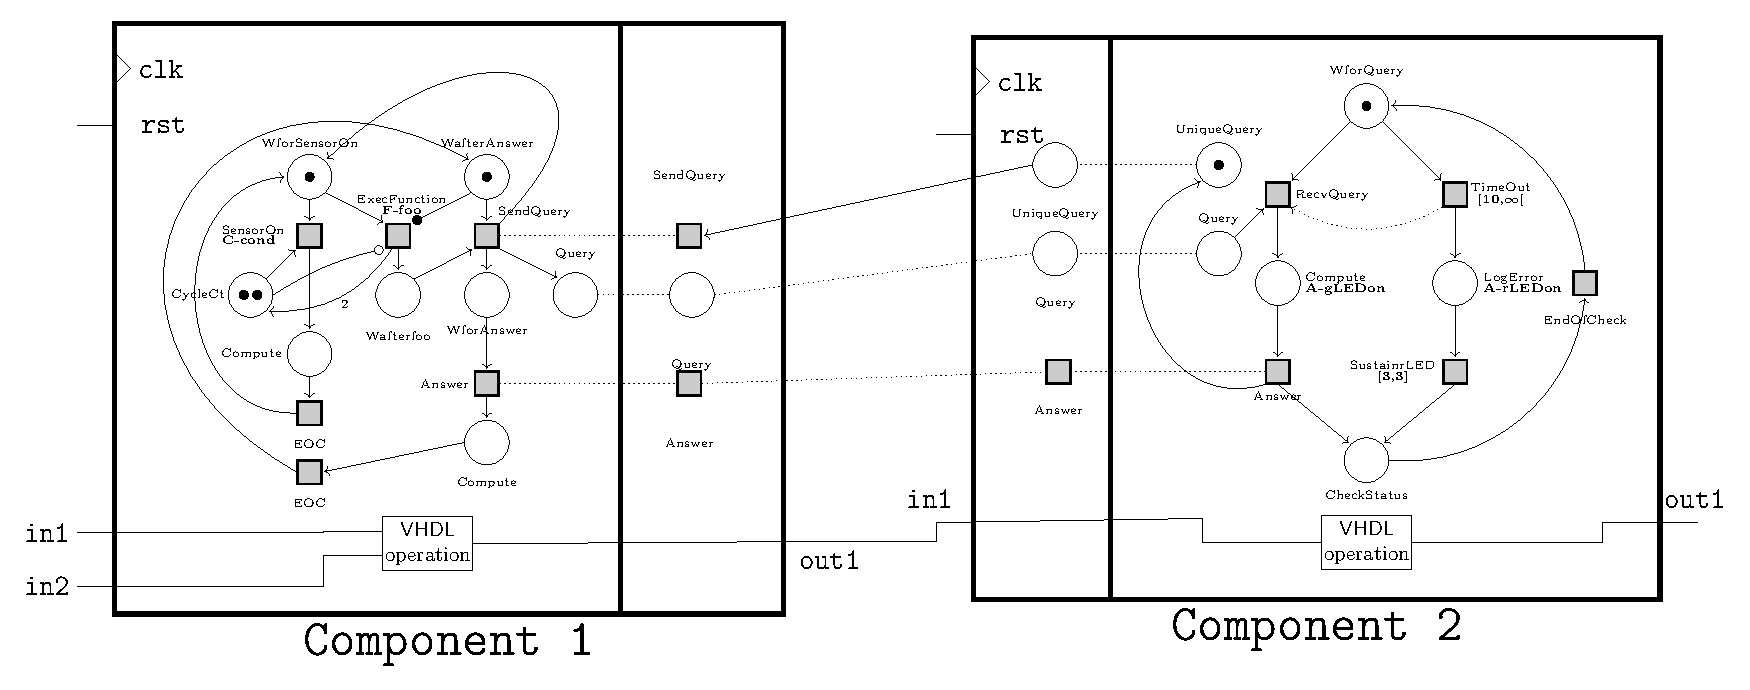
\includegraphics[keepaspectratio=true,width=\textwidth]{abs-model.eps}
\caption[An example of model of digital system in \hilecop{}.]{A
  component-based model of digital system in \hilecop{}.}
\label{fig:abs-model}
\end{figure}

In \hilecop{}'s high-level formalism, a model of digital system is
composed of boxes that represent the different components of the
system. Figure~\ref{fig:abs-model} gives an example of such a model.
The internal behavior of each component is defined by a SITPN model.
The elements of a component's internal behavior can be connected to
the elements of another component's behavior through an interface. Two
elements are either connected through a place-transition (or
transition-place) arc, or through a fusion arc (dotted line in
Figure~\ref{fig:abs-model}). While designing a component, an engineer
can also define input and output ports in the component interface,
declare internal signals, and perform operations over the ports and
internal signals by writing \vhdl{} code. All the \vhdl{} code defined
in this way will be copied as is in the output \vhdl{} design during
the model-to-text transformation. Note that all components declare a
clock and a reset signal (cf. \texttt{clk} and \texttt{rst} in
Figure~\ref{fig:abs-model}). These signals are related to the
synchronous execution of the system in the generated circuit.

Before being transformed into \vhdl{} code, the model is flattened
down (cf. Step \circled{1} to step \circled{2} in
Figure~\ref{fig:hilecop-wf}). All component structures are removed,
and the result is one global SITPN model. During this flattening step,
all elements that were connected through fusion arcs are merged
together. Figure~\ref{fig:impl-model} presents the global SITPN model
resulting from the flattening of the component-based model of
Figure~\ref{fig:abs-model}.

\begin{figure}[H]
\centering
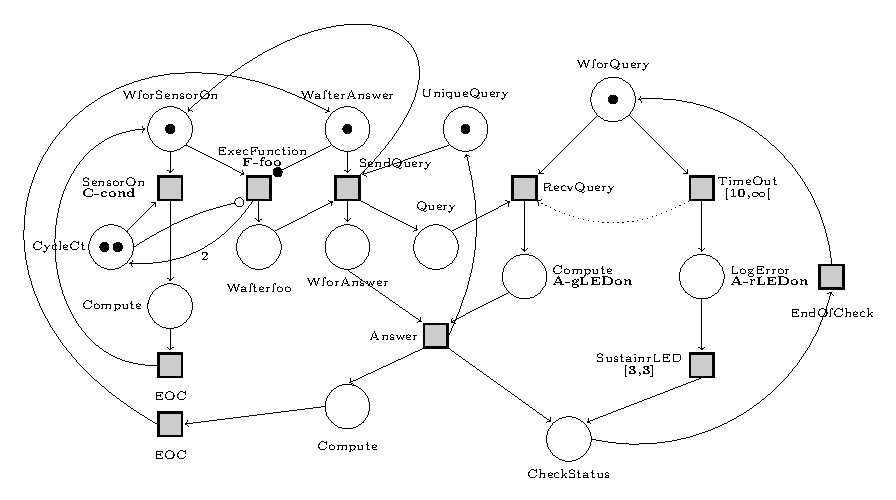
\includegraphics[keepaspectratio=true,width=\textwidth] {impl-model.eps}
\caption[Global Petri net model.]{A global Petri net model obtained
  after the flattening of a \hilecop{} high-level model.}
\label{fig:impl-model}
\end{figure}

SITPNs are a combination of multiple classes of PNs, namely: extended
PNs, generalized PNs, interpreted PNs, time PNs and PNs with
priorities. A generalized Petri net admits the weight of its arcs to
be a natural number instead of the default value of one (i.e. when no
number is written above the arc). An extended Petri net introduces two
kinds of place-transition arcs, the \textit{inhibitor} arc,
characterized by a white circle head, and the \textit{test} arc, which
has a black circle head. These arcs add conditions to the firing of a
connected transition, however, they do not cause tokens to be removed
from input places at firing time. In Figure~\ref{fig:impl-model}, the
arc from place CycleCt to transition ExecFunction is an inhibitor arc,
and the arc from place WafterAnswer to ExecFunction is a test arc.
Now, let us introduce more specifically the class of interpreted PNs,
time PNs and PNs with priorities.

\paragraph{Interpreted Petri nets (IPNs)}
% As stated in \cite{David1994}, Interpreted Petri Nets (IPN) ``can be
% applied to various interpretations according to the use wished to be
% made of it''.
In its general definition \cite{David1994}, an IPN is associated with
a finite set of variables $V$, a finite set of operations $O$, and a
finite set of conditions $C$. Operations of the $O$ set are associated
with places and triggered when the places become marked. The execution
of operations affects the value of the variables, and the value of
conditions depends on Boolean expressions computed upon the variables.
Conditions are associated with transitions and become involved in the
firing process.  In the \hilecop{} version of
IPNs, % refines the concepts of the general
% definition. In this version, 
the set of variables corresponds to the set of \vhdl{} signals that
are handled by the model; a signal can be an input port, an output
port or an internal signal of the modeled hardware circuit. The
operations, implemented by \vhdl{} procedures, are separated in two
kinds, namely: actions and functions. Actions (or continuous
operations) are associated to the places; all the actions associated
to a place $p$ are activated as long as $p$ is marked (i.e. as long as
$p$ holds a token). Functions (or discrete operations) are associated
to the transitions; when a transition $t$ is fired, all functions
associated to $t$ are executed once. In Figure \ref{fig:impl-model},
\textbf{C-cond} is a condition associated to the transition SensorOn;
\textbf{F-foo} is a function associated to the transition
ExecFunction; \textbf{A-gLEDon} and \textbf{A-rLEDon} are two actions
associated to the Compute and LogError places.

\paragraph{Time Petri nets (TPNs)}

In a TPN, time intervals can be associated to transitions, along with
a dynamic time counter value. Thus, the firing of a transition must
happen in a given time window. In the \hilecop{} version of TPNs, time
intervals are of the form $[a, b]$, where $a\in\mathbb{N}^{*}$ and
$b\in\mathbb{N}^{*}\sqcup\{\infty\}$.  In Figure~\ref{fig:impl-model},
transitions SustainrLED and TimeOut are both associated with time
intervals.

\paragraph{Petri nets with priorities}

Two transitions are in structural conflict if they have a common input
place connected through a \textit{basic} arc (i.e. neither inhibitor
nor test arc). When two transitions in structural conflict are firable
at the same time and if the firing of one of the transitions disables
the other, then, the conflict becomes \textit{effective}. In a Petri
net with priorities, it is possible to specify a firing priority in
the case where the conflict between two transitions becomes
effective. In that case, the transition with the highest firing
priority will always be fired first. In Figure \ref{fig:impl-model},
the fact that transition TimeOut has a higher firing priority than
transition RecvQuery is graphically represented by a dotted arrow. \\

\noindent{}Now let us formally introduce the structure of SITPNs:

\begin{definition}[SITPN]
  \label{def:sitpn}
  A synchronously executed, extended, generalized, interpreted, and
  time Petri net with priorities is a tuple
  ${<}P,T,pre,post,M_0,{\succ},\mathcal{A},\mathcal{C},\mathcal{F},
  \mathbb{A},\mathbb{C},\mathbb{F},{I_s}{>}$, where we have:
  % 
  \begin{enumerate}
  \item $P=\{p_0,\ldots,p_n\}$, a finite set of places.
  \item $T=\{t_0,\ldots,t_m\}$, a finite set of transitions.
  \item
    $pre\in{}P\rightarrow{}T\nrightarrow(\mathbb{N}^{*}\times\{\mathtt{basic},\mathtt{inhib},\mathtt{test}\})$,
    the function associating a weight and a type to place-transition
    edges.
  \item $post\in{}T\rightarrow{}P\nrightarrow\mathbb{N}^{*}$, the
    function associating a weight to transition-place edges.
  \item $M_0\in{}P\rightarrow\mathbb{N}$, the initial marking of the SITPN.
  \item $\succ\subseteq{}(T\times{}T)$, the priority relation, which
    is a strict partial order over the set of transitions.
  \item $\mathcal{A}=\{a_0,\ldots,a_i\}$, a finite set of continuous actions.
  \item $\mathcal{F}=\{f_0,\ldots,f_k\}$, a finite set of functions.
  \item $\mathcal{C}=\{c_0,\ldots,c_j\}$, a finite set of conditions.
  \item $\mathbb{A}$ $\in$ ${}P$ $\rightarrow$ $\mathcal{A}$
    $\rightarrow$ $\mathbb{B}$, the function associating actions to
    places.  $\forall{}p\in{}P$, $\forall{}a\in\mathcal{A}$,
    $\mathbb{A}(p,a)=\mathtt{true}$, if $a$ is associated to $p$,
    $\mathbb{A}(p,a)=\mathtt{false}$ otherwise.
  \item $\mathbb{F}\in{}T\rightarrow\mathcal{F}\rightarrow\mathbb{B}$,
    the function associating functions to transitions.
    $\forall{}t\in{}T,~\forall{}f\in\mathcal{F},$
    $\mathbb{F}(t,f)=\mathtt{true}$, if $f$ is associated to $t$,
    $\mathbb{F}(t,f)=\mathtt{false}$ otherwise.
    
  \item $\mathbb{C} \in T \rightarrow \mathcal{C} \rightarrow\{-1,0,1\}$, the
    function associating conditions to transitions.
    $\forall t \in T$, $\forall c \in \mathcal{C}$,
    $\mathbb{C}(t,c)=1$, if $c$ is associated to $t$,
    $\mathbb{C}(t,c)=-1$, if $\bar{c}$ is associated to $t$,
    $\mathbb{C}(t,c)=0$ otherwise.
  \item
    $I_s\in{}T\nrightarrow(\mathbb{N}^{*}\times(\mathbb{N^{*}}\sqcup\{\infty\}))$,
    the partial function associating time intervals to transitions.
  \end{enumerate}
\end{definition}

In Definition~\ref{def:sitpn}, we do not consider the set of \vhdl{}
signals manipulated by a SITPN model. As a consequence, the structure
holds neither the association between conditions and Boolean
expressions, and nor the association between actions/functions and
operations (i.e. \vhdl{} procedures that act upon signal values).  In
this simplified version of the SITPN structure, conditions, actions
and functions are only considered as finite sets of indexed elements
associated with the places and transitions of a SITPN.

\subsection{Synchronous execution semantics}
\label{subsec:hpn-particularities}

The SITPN semantics describes the evolution of the state of a SITPN
through a given number of clock cycles; thus, we must first define the
SITPN state structure. In what follows, for a given $sitpn\in{}SITPN$,
$T_i$ denotes the definition domain of $I_s$, i.e. the set of
transitions associated with a time interval, referred to as
\textit{time transitions}.

\begin{definition}[SITPN State]
  \label{def:sitpnstate}
  For a given $sitpn\in{}SITPN$, let $S(sitpn)$ be the set of possible
  states of $sitpn$. An SITPN state $s\in{}S(sitpn)$ is a tuple
  ${<}M,I,reset_t,ex,cond{>}$, where:
  \begin{enumerate}
  \item $M\in{}P\rightarrow\mathbb{N}$ is the current marking of
    $sitpn$.
  \item\label{item:sitpn-state-tc} $I\in{}T_i{}\rightarrow\mathbb{N}$
    is the function mapping time transitions to their current time
    counter value.
  \item\label{item:sitpn-state-rst}
    $reset_t\in{}T_i\rightarrow\mathbb{B}$ is the function mapping
    time transitions to time counter reset orders (defined as
    Booleans).
  \item $ex\in{}\mathcal{A}\sqcup\mathcal{F}\rightarrow\mathbb{B}$ is
    the function representing the current activation (resp. execution)
    state of actions (resp. functions).
  \item $cond\in\mathcal{C}\rightarrow\mathbb{B}$ is the function representing the
    current value of conditions (defined as Booleans).
  \end{enumerate}
\end{definition}

As described in Definition~\ref{def:sitpnstate}, the state of a SITPN
is characterized by its marking, the value of time counters, the reset
orders assigned to time counters, the execution/activation status of
actions/functions (Boolean values), and the value of conditions (also
Boolean). Regarding actions and functions, note that we are only
interested in the fact that a given action/function is
activated/executed but no more in actually executing the associated
operation.\\

Before describing the SITPN state transition relation, we need to
formally define the sensitization of a given transition by a given
marking, and the firability of a given transition with respect to a
given SITPN state.

\begin{definition}[Sensitization]
  \label{def:sens}
  A transition $t\in{}T$ is said to be sensitized, or enabled, by a
  marking $M$, which is noted $t\in{}Sens(M)$, if
  $\forall{}p\in{}P,\forall\omega\in\mathbb{N}^{*},~\big(pre(p,t)=(\omega,\mathtt{basic})\vee{}pre(p,t)=(\omega,\mathtt{test})\big)\Rightarrow{}M(p)\ge{}\omega$,
  and $pre(p,t)=(\omega,\mathtt{inhib})\Rightarrow{}M(p)<{}\omega$.
\end{definition}

\begin{definition}[Firability]
  \label{def:firable}
  A transition $t\in{}T$ is said to be firable at a state
  $s={<}M,I,reset_t,ex,cond{>}$, which is noted $t\in{}Firable(s)$, if
  $t\in{}Sens(M)$, and $t\notin{}T_i$ or $I(t)\in{}I_s(t)$, and
  $\forall c \in \mathcal{C}, \mathbb{C}(t, c) = 1 \Rightarrow cond(c)
  = 1$ and $\mathbb{C}(t, c) = -1 \Rightarrow cond(c) = 0$.
\end{definition}


All transitions that are firable at a given state are possible members
of the set of fired transitions. A firable transition is also a fired
transition if it is still enabled by the \textit{residual} marking,
that is, the marking resulting from the firing of transitions with a
higher priority.  Priorities are defined with the priority relation,
which is a part of the SITPN structure.  As illustrated in
Figure~\ref{fig:resid-marking}, to determine which transitions of
$t_0$, $t_1$ and $t_2$ are fired, a \emph{residual marking} is
computed by following the priority order. For each transition of the
group $t_0$, $t_1$ and $t_2$, the residual marking represents the
remaining tokens in $p_0$ after the firing of transitions with a
higher firing priority.  Thus, the recursive definition of the set of
fired transitions at a given SITPN state is as follows:

\begin{definition}[Fired]
  \label{def:fired}
  A transition $t\in{}T$ is said to be fired at the SITPN state
  $s={<}M,I,reset_t,ex,$ $cond{>}$, which is noted $t\in{}Fired(s)$,
  if $t\in{}Firable(s)$ and
  $t\in{}Sens\big(M-\sum\limits_{t_i\in{}Pr(t)}pre(t_i)\big)$, where
  $Pr(t)=\{t_i~|~t_i\succ{}t\wedge{}t_i\in{}Fired(s)\}$.
\end{definition}


\begin{figure}[H]
  \centering
  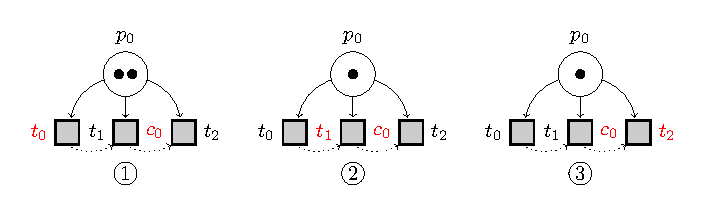
\includegraphics[keepaspectratio=true, width=.8\textwidth]{resid-marking.eps}
  \caption[Computation of the residual marking of a group of
  conflicting transitions.]{Computation of the residual marking for a
    group of conflicting transitions. At \circled{1}
    (resp. \circled{2} and \circled{3}), place $p_0$ holds the
    residual marking for transition $t_0$ (resp. $t_1$ and
    $t_2$). Condition $c_0$ appears in normal font to indicate that
    its current value is \texttt{false}.}
  \label{fig:resid-marking}
\end{figure}

Note that the computation of the residual marking only involves the
consumption phase of the firing process; tokens are withdrawn from
places, but none are generated.

Note also that there is an equivalence between being firable and being
fired at a given state when considering a \textit{top-priority}
transition, i.e. a transition for which there exists no transition
with a higher firing priority.

\paragraph{The state transition relation}

The evolution of the state of a SITPN is \textit{synchronized} with
the rising edge event and the falling edge event of a clock signal.
The rising edge event triggers the marking update, the computation of
time counter reset orders, and the execution of functions. On the
falling edge of the clock signal, the value of conditions are
updated. As the SITPN structure does not hold the link between Boolean
expressions computed over \vhdl{} signals and conditions, the update
of condition values is represented by the injection of fresh Boolean
values coming from an environment. Moreover, the falling edge event
triggers the evolution of the time counter values; values are
incremented, reset, or stalling in the case where a time counter has
reached the upper bound of its associated time interval. Finally, all
actions associated with marked places are
activated. Figure~\ref{fig:sitpn-state-exec} gives an example of the
evolution of the state of a given SITPN through one clock cycle,
happening in the middle of other clock cycles.

\begin{figure}[H]
  \centering
  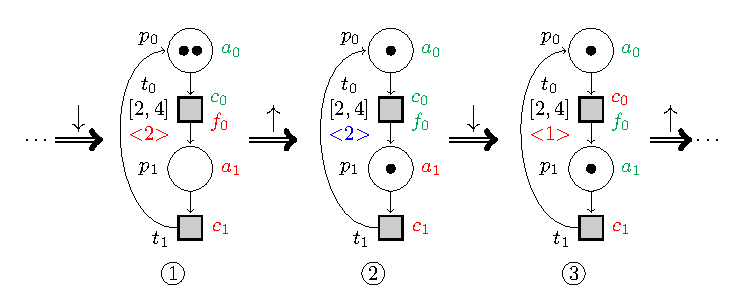
\includegraphics[keepaspectratio=true, width=.8\textwidth]{sitpn-state-evol.eps}
  \caption[Evolution of an SITPN over one clock cycle.]{The evolution
    of a SITPN over one clock cycle. Conditions (i.e. $c_0$ and $c_1$)
    appear in bold font when \texttt{true}; actions (i.e. $a_0$ and
    $a_1$) and functions ($f_0$) appear in bold font when
    activated/executed; time counters appear between diamond brackets,
    and are represented between inverted brackets when they are
    subject to a reset order.}
  \label{fig:sitpn-state-exec}
\end{figure}

In Figure~\ref{fig:sitpn-state-exec}, from Step~1 to Step~2, the
rising edge of the clock signal triggers the firing of transition
$t_0$. As transition $t_0$ is firable and is not in effective conflict
with other transitions, $t_0$ is fired: one token is consumed in place
$p_0$ and one token is produced in place $p_1$. Also, function $f_0$
is executed at the occurrence of the rising edge of the clock signal,
and thus, $f_0$ appears in bold font at Step~2. Consequently to the
firing of $t_0$, a reset order is sent to the time counter of $t_0$,
and it appears between inverted brackets at Step~2. From Step~2 to
Step~3, the falling edge updates the action activation status: $a_0$
stays activated as place $p_0$ is still marked; $a_1$ becomes newly
activated as place $p_1$ just received a token. Time counters are
updated: $t_0$'s time counter is set to zero as the transition
previously received a reset order. However, as $t_0$ is still enabled
by the new marking, its time counter is incremented. Thus, the
resulting time counter value at Step~3 is of one (i.e. result of reset
plus increment). Also, the environment provides a new value to each
condition. As a consequence, condition $c_0$ takes the value
\texttt{false} and condition $c_1$ keeps the same value.

We formalize the evolution of a SITPN state synchronized with the
events of a clock signal with the following state transition relation:

\begin{definition}[SITPN state transition]
  \label{def:semantics}
  For a given $sitpn\in{}SITPN$, the SITPN state transition relation
  $\rightarrow\subseteq{}(\mathbb{N}\rightarrow\mathcal{C}\rightarrow\mathbb{B})\times{}\mathbb{N}\times{}S(sitpn)\times{}\{\uparrow,\downarrow\}\times{}S(sitpn)$
  is noted as follows $E_c,\tau\vdash{}s\xrightarrow{clk}s'$, where
  $E_c\in\mathbb{N}\rightarrow\mathcal{C}\rightarrow\mathbb{B}$ is an
  environment that maps the conditions of $sitpn$ to a Boolean value
  at a given clock count, $\tau\in\mathbb{N}$ is the current clock
  count, $s,s'\in{}S(sitpn)$ are two states of $sitpn$ and
  $clk\in\{\uparrow,\downarrow\}$ is a clock event. The relation is
  defined by the two following rules:
  
  \begin{itemize}
  \item
    $\forall{}E_c\in\mathbb{N}\rightarrow\mathcal{C}\rightarrow\mathbb{B}$,
    $\forall\tau\in\mathbb{N}$, $\forall{}s,s'\in{}S(sitpn)$, we have
    $E_c,\tau\vdash{}s\xrightarrow{\uparrow}s'$, where
    $s=<M,I,reset_t,ex,cond>$ and $s'=<M',I,reset_t',ex',cond>$, if:
    \begin{enumerate}
    \item\label{it:new-marking} $M'$ is the new marking resulting
      from
      the firing of all the transitions contained in $Fired(s)$, i.e.:
      \begin{equation*}
        \forall{}p\in{}P,~M'(p)=M(p)-\sum\limits_{t\in{}Fired(s)}pre(p,t)+\sum\limits_{t\in{}Fired(s)}post(t,p).
      \end{equation*}
      
    \item\label{it:reset-order} A time transition receives a reset
      order if it is fired at state $s$, or, if there exists a place
      $p$ connected to $t$ by a \texttt{basic} or \texttt{test arc}
      and at least one output transition of $p$ is fired and the
      transient marking of $p$ disables $t$; no reset order is sent
      otherwise:
      \begin{equation*}
        \begin{split}
          \forall{}t\in{}T_i,&~t\in{}Fired(s) \\
                             &\lor\big(\exists{}p\in{}P,\omega\in\mathbb{N}^{*}, \\
                             &\quad\quad{}[pre(p,t)=(\omega,\mathtt{basic})\lor{}pre(p,t)=(\omega,\mathtt{test})] \\
                             &\quad\quad\land\sum\limits_{t_i\in{}Fired(s)}pre(p,t_i)>0 \\
                             &\quad\quad\land{}M(p)-\sum\limits_{t_i\in{}Fired(s)}pre(p,t_i)<\omega\big)\\
                             & \Rightarrow{}reset'_t(t)=\mathtt{true}~and~reset'_t(t)=\mathtt{false}~otherwise.  \\
        \end{split}
      \end{equation*}
      
    \item\label{it:exec-fun} All functions associated with at least one fired transition are executed, i.e:
      \begin{equation*}
        \forall{}f\in{}\mathcal{F},~ex'(f)=\sum\limits_{t\in{}Fired(s)}\mathbb{F}(t,f).
      \end{equation*}
    \end{enumerate}
    
  \item
    $\forall{}E_c\in\mathbb{N}\rightarrow\mathcal{C}\rightarrow\mathbb{B}$,
    $\forall\tau\in\mathbb{N}$, $\forall{}s,s'\in{}S(sitpn)$, we have
    $E_c,\tau\vdash{}s\xrightarrow{\downarrow}s'$, where
    $s=<M,I,reset_t,ex,cond>$ and $s'=<M,I',reset_t,ex',cond'>$, if:
    \begin{enumerate}[resume]
    \item\label{it:cond-env} $cond'$ is the function giving the
      (Boolean) values of conditions that are extracted from the
      environment $E_c$ at the clock count
      $\tau$, i.e.:
      \begin{equation*}
        \forall{}c\in{}\mathcal{C},~cond'(c)=E_c(\tau,c).
      \end{equation*}
      
    \item\label{it:activate-actions} All the actions associated
      with at least one
      marked place in the marking $M$ are activated, i.e.:
      \begin{equation*}
        \forall{}a\in{}\mathcal{A},~ex'(a)=\sum\limits_{M(p)>0}\mathbb{A}(p,a).
      \end{equation*}
    \item\label{it:reset-counters} All the time transitions that are
      sensitized by the marking $M$ and received the order to reset
      their time intervals, have their time counter reset and
      incremented, i.e.:
      \begin{equation*}
        \forall{}t\in{}T_i,~t\in{}Sens(M)\land{}reset_t(t)=\mathtt{true}
        \Rightarrow{}I'(t)=1.
      \end{equation*}
      
    \item\label{it:inc-counters} All the time transitions that are
      sensitized by the marking $M$, and
      did not receive a reset order, increment their time counters if time counters are still active, i.e.:
      \begin{equation*}
        \begin{split}
          \forall{}t\in{}T_i,~&t\in{}Sens(M)\land{}reset_t(t)=\mathtt{false}\land{}[I(t)\le{}u(I_s(t))\lor{}u(I_s(t))=\infty]\\
                              & \Rightarrow{}I'(t)=I(t)+1. \\
        \end{split}
      \end{equation*}
    \item\label{it:locked-counters} All the time transitions
      verifying the same
      conditions as above, but with locked counters, keep having locked counters (values are stalling), i.e.:        
      \begin{equation*}
        \begin{split}
          \forall{}t\in{}T_i,~&t\in{}Sens(M)\land{}reset_t(t)=\mathtt{false}\land{}I(t)>{}u(I_s(t))\land{}u(I_s(t))\neq\infty\\
                              & \Rightarrow{}I'(t)=I(t).\\
        \end{split}
      \end{equation*}
      
    \item\label{it:reset-not-sens} All the time transitions disabled by the marking $M$ have their time counters set to zero, i.e.:
      \begin{equation*}
        \forall{}t\in{}T_i,~t\notin{}Sens(M)\Rightarrow{}I'(t)=0.
      \end{equation*}
    \end{enumerate}
    
  \end{itemize}
\end{definition}

Premises~\ref{it:new-marking} to \ref{it:exec-fun} describe the SITPN
state evolution at the rising edge of the clock signal.
Premise~\ref{it:new-marking} corresponds to the marking update. The
computation of the new marking uses the set of fired transitions at
state $s$, i.e. $Fired(s)$. Premise~\ref{it:exec-fun} deals with the
update of the function execution status. Premise~\ref{it:reset-order}
computes the reset orders for time transitions. There are two cases
where a time transition receives the order to reset its time
counter. First, if the transition is one of the fired transitions at
state $s$, then its time counter must be reset on the next falling
edge. Second, if the transition is disabled in a \emph{transient}
manner, then its time counter must also be reset.

Premises~\ref{it:cond-env} to \ref{it:reset-not-sens} describe the
SITPN state evolution at the falling edge of the clock
signal. Premises~\ref{it:cond-env} and \ref{it:activate-actions} deal
with the update of condition values and the activation status of
actions. Note that in Premise~\ref{it:activate-actions} (and also in
Premise~\ref{it:exec-fun}), the sum expression corresponds to the
Boolean sum expression, i.e. the application of the \texttt{or}
operator over the elements of the iterated
set. Premises~\ref{it:reset-counters}, \ref{it:inc-counters},
\ref{it:locked-counters} and \ref{it:reset-not-sens} focus on the
update of time counter values.  In Premise~\ref{it:inc-counters} of
the SITPN semantics, the \emph{active} time counters refer to the time
counters that have not yet overreached the upper bound of their
associated time interval. Of course, a time counter is always active
when the upper bound is infinite. In Premise~\ref{it:locked-counters},
the \emph{locked} time counters refer to the time counters that have
overreached the upper bound of their associated time interval. Of
course, time counters can never be locked in the presence of an
infinite upper bound. In Premises~\ref{it:inc-counters} and
\ref{it:locked-counters}, for a given time interval $i$, $u(i)$
denotes the upper bound of the time interval, and $l(i)$ denotes the
lower bound of the time interval.\\

To give a small-step execution semantics to a SITPN model, we have
defined an execution relation that binds a given SITPN model to an
execution trace, i.e. a time-ordered list of states. The execution
trace is built for a given number of clock cycles, starting from the
initial state of the SITPN model.  The initial state of a SITPN model
is formally defined as follows:

\begin{definition}[Initial state]
  \label{def:sitpn-init-state}
  For a given $sitpn\in{}SITPN$, $s_0\in{}S(sitpn)$ is the initial
  state of $sitpn$, such that
  $s_0=<M_0,O_\mathbb{N},O_\mathbb{B},O_\mathbb{B},O_\mathbb{B}>$,
  where $M_0$ is the initial marking of the SITPN, $O_\mathbb{N}$ is a
  function that always returns 0, $O_\mathbb{B}$ is a function that
  always returns \texttt{false}.
\end{definition}

Here are the definitions of the SITPN execution and the SITPN full
execution relations.

\begin{definition}[SITPN execution]
  \label{def:sitpn-exec}
  For a given $sitpn\in{}SITPN$, a starting state $s\in{}S(sitpn)$, a
  clock cycle count $\tau\in\mathbb{N}$, and an environment
  $E_c\in\mathbb{N}\rightarrow{}\mathcal{C}\rightarrow{}\mathbb{B}$,
  $sitpn$ yields the execution trace $\theta$ from starting state $s$,
  written $E_c,\tau\vdash{}sitpn,s\rightarrow{}\theta$, by following
  the two rules below:
  
  \begin{tabular}{@{}l}
    % {\fontsize{10}{12}\selectfont
    % \textsc{ExecutionEnd}} \\
    {\begin{prooftree}
        \infer0 {E_c,0\vdash{}sitpn,s\rightarrow{}[~]}
      \end{prooftree}} 
  \end{tabular}
  \begin{tabular}{@{}l}
    % {\fontsize{10}{12}\selectfont
    % \textsc{ExecutionLoop}} \\    
    {\begin{prooftree}[template={\inserttext}]

        \hypo{$E_c,\tau\vdash{}s\xrightarrow{\uparrow}s'$}
        \infer[no rule]1{$E_c,\tau\vdash{}s'\xrightarrow{\downarrow}s''$}
        \hypo{$E_c,\tau-1\vdash{}sitpn,s''\rightarrow{}\theta$}
        
        \infer2[$\tau>0$]{$E_c,\tau\vdash{}sitpn,s\rightarrow{}(s' :: s'' :: \theta)$}
      \end{prooftree}} 
  \end{tabular}
\end{definition}

The first rule of Definition~\ref{def:sitpn-exec} states that the
execution of a $sitpn\in{}SITPN$, starting from a state
$s\in{}S(sitpn)$ in the environment
$E_c\in{}\mathbb{N}\rightarrow\mathcal{C}\rightarrow\mathbb{B}$,
yields an empty execution trace if the clock count comes down to $0$.
The second rule describes how the execution trace related to the
execution of a $sitpn\in{}SITPN$ is built in the case where the clock
count $\tau$ is greater than zero. The final execution trace is
composed of a head state $s'$, followed by state $s''$ and the tail
trace $\theta$. The $::$ operator builds a new trace by adding a new
element at the head of an existing trace. Starting from state $s$,
$sitpn$ reaches state $s'$ after a rising edge event; then from state
$s'$, it reaches state $s''$ after a falling edge event, i.e. from $s$
to $s''$, a whole clock cycle is performed.  Finally, the execution
trace $\theta$ is obtained through the recursive call to the SITPN
execution relation where $sitpn$ is executed during $\tau-1$ cycles
starting from state $s''$.

\begin{definition}[SITPN full execution]
  \label{def:sitpn-full-exec}
  For a given $sitpn\in{}SITPN$, a clock cycle count
  $\tau\in\mathbb{N}$, and an environment
  $E_c\in\mathbb{N}\rightarrow{}\mathcal{C}\rightarrow{}\mathbb{B}$,
  $sitpn$ yields the execution trace $\theta$ starting from its
  initial state $s_0\in{}S(sitpn)$ (as defined in
  Definition~\ref{def:sitpn-init-state}), written
  $E_c,\tau\vdash{}sitpn\rightarrow{}\theta$, by following the two
  rules below:
  
  \begin{tabular}{@{}l}
    % {\fontsize{10}{12}\selectfont\textsc{FullExec0}} \\
    {\begin{prooftree}[template={\inserttext}]
        
        \infer0{$E_c,0\vdash{}sitpn\xrightarrow{full}[s_0]$}
      \end{prooftree}} 
  \end{tabular}
  \begin{tabular}{l}
    % {\fontsize{10}{12}\selectfont\textsc{FullExecCons}} \\
    {\begin{prooftree}[template={\inserttext}]
        \hypo{$E_c,\tau\vdash{}s_0\xrightarrow{\downarrow}s$}
        \hypo{$E_c,\tau-1\vdash{}sitpn,s\rightarrow\theta_s$}
        \infer2[$\tau>0$]{$E_c,\tau\vdash{}sitpn\xrightarrow{full}(s_0 :: s_0 :: s :: \theta_s)$}
      \end{prooftree}} 
  \end{tabular}

\end{definition}

The first rule of the Definition~\ref{def:sitpn-full-exec} appeals to
the SITPN execution relation
(i.e. Definition~\ref{def:sitpn-exec}). However, the definition of the
SITPN full execution relation is necessary because the first cycle of
execution, starting from the initial state $s_0$, is particular. As a
matter of fact, no transition is fired during the first rising
edge. Thus, the first rising edge does not change the initial state
$s_0$. This is why, in the second rule, the execution trace begins
with two states $s_0$, thus representing the idle first rising edge.

\subsection{Well-definition of a SITPN}
\label{sec:sitpn-wd}

The synchronous execution semantics of SITPNs implies that all
transitions are fired at the same time. In
Figure~\ref{fig:double-consum}, transitions $t_0$ and $t_1$ are both
firable before the rising edge event. As no priority relation is drawn
between the two conflicting transitions, they are both fired at the
occurrence of the event. The system acts as if two tokens were
available in place $p_0$, one for the firing of $t_0$ and another for
the firing of $t_1$.

\begin{figure}[H]
  \centering
  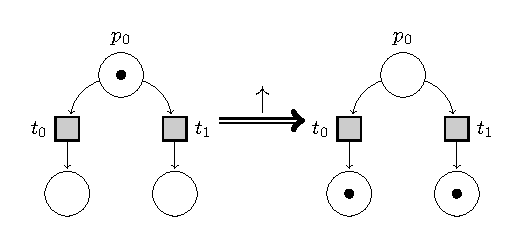
\includegraphics[keepaspectratio=true, width=.5\textwidth]{double-consum.eps}
  \caption[Double consumption of token in a SITPN.]{Double consumption
    of one token in a SITPN. On the left side, the current marking
    before the firing of $t_0$ and $t_1$; on the right side, the
    marking resulting from the firing of $t_0$ and $t_1$. The arrow
    indicates the occurrence of a rising edge that triggers the firing
    process.}
  \label{fig:double-consum}
\end{figure}

In the context of a SITPN, a branching like the one of
Figure~\ref{fig:double-consum}, normally interpreted as a disjunctive
branching, takes the semantics of a conjunctive branching if no
priority is specified between the conflicting transitions. To avoid
the phenomenon of ``double consumption'' of tokens, we enforce the
resolution of any structural conflict by means of mutual exclusion or
through the application of priorities. This policy about the
resolution of structural conflicts is part of the definition of a
\emph{well-defined} SITPN. We must be able to decide which transition
in a conflicting pair will be fired when the conflict becomes
effective. Thus, we give place-centered definition of a group of
transitions in conflict:

\begin{definition}[Conflicting group of transitions]
  \label{def:cgroup}
  For a given $sitpn\in{}SITPN$, the conflicting transitions of a
  given place $p$, noted $conflict(p)$, are all transitions related to
  $p$ with a \texttt{basic} place-transition arc,
  i.e.
  $conflict(p)=\{t\in{}T~\vert~\exists{}\omega\in\mathbb{N}^{*},~pre(p,t)=(\omega,\mathtt{basic})\}$.
\end{definition}

This view of a conflict group reflects the place-centered view of
conflicts as implemented in the \vhdl{} code generated by the
model-to-text transformation.  Figure~\ref{fig:conflict-groups} shows
the conflict group related to place $p_0$ and $p_1$, namely:
$\{t_0,t_3\}$ and $\{t_1,t_4\}$.

\begin{figure}[H]
  \centering
  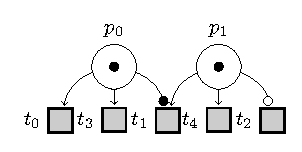
\includegraphics[keepaspectratio,width=.3\linewidth]{conflict-groups.eps}
  \caption[An example of two separate conflict groups.]{An example of
    two separate conflict groups, namely: $\{t_0,t_3\}$ and
    $\{t_1,t_4\}$.}
  \label{fig:conflict-groups}
\end{figure}

In a well-defined SITPN, all conflicts in a conflict group must be
considered, i.e. for all pair of transitions in the group the conflict
must be solved. When the conflict between a pair of transitions
becomes effective, there are two ways to be sure that only one
transition will be fired. The first way is to define a firing order
through a priority relation. The second way is to use a mean of mutual
exclusion. A mean of mutual exclusion ensures that the two transitions
of a conflicting pair will never be firable at the same time. We only
consider two ways of mutual exclusion, namely: mutual exclusion with
complementary conditions and mutual exclusion with inhibitor arcs.

\begin{definition}[Mutual exclusion with complementary conditions]
  \label{def:mutex-conds}
  Given two conflicting transitions $t_0$ and $t_1$, $t_0$ and $t_1$
  are in mutual exclusion with complementary conditions if there
  exists $c\in\mathcal{C}$ such that
  $(\mathbb{C}(t_0,c)=1\land{}\mathbb{C}(t_1,c)=-1)$ or
  $(\mathbb{C}(t_0,c)=-1\land{}\mathbb{C}(t_1,c)=1)$.
\end{definition}

\begin{definition}[Mutual exclusion with an inhibitor arc]
  \label{def:mutex-inhib} Given two conflicting transitions $t_0$ and
  $t_1$, $t_0$ and $t_1$ are in mutual exclusion with an inhibitor arc
  if there exists $p\in{}P$ and $\omega\in{}\mathbb{N}^{*}$ such that
  $(pre(p,t_0)=(\omega,\mathtt{basic})\lor{}pre(p,t_0)=(\omega,\mathtt{test}))\land{}pre(p,t_1)=(\omega,\mathtt{inhib})$
  or
  $(pre(p,t_1)=(\omega,\mathtt{basic})\lor{}pre(p,t_1)=(\omega,\mathtt{test}))\land{}pre(p,t_0)=(\omega,\mathtt{inhib})$.
\end{definition}

Figure~\ref{fig:mutex} illustrates the two means of mutual exclusion
that can be applied to solve a conflict between two transitions.

\begin{figure}[H]
  \centering
  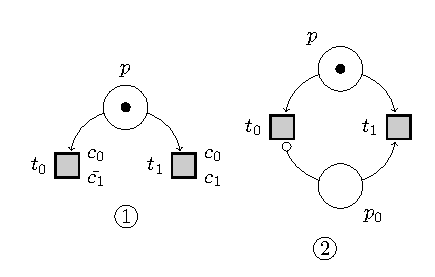
\includegraphics[keepaspectratio,width=.45\linewidth]{mutex.eps}
  \caption[Examples of conflicting transitions in mutual exclusion.]{
    Examples of conflicting transitions in mutual exclusion. At
    \circled{1}, an example of mutual exclusion with complementary
    conditions; at \circled{2}, an example of mutual exclusion with an
    inhibitor arc.}
  \label{fig:mutex}
\end{figure}

In Figure~\ref{fig:mutex}, in situation \circled{1}, condition $c_1$
is associated to $t_1$ and the complementary condition is associated
to $t_0$ thus creating the mutual exclusion. In situation \circled{2},
the arcs $(p_0,t_0)$ and $(p_0,t_1)$ ensure the mutual exclusion
between transitions $t_0$ and $t_1$. Note that in the structure of
mutual exclusion with an inhibitor arc, the weight of the inhibitor
arc and of the one of the basic or test arc must be the same;
otherwise, the mutual exclusion is not effective.\\

\noindent{}A well-defined SITPN is defined as follows:

\begin{definition}[Well-defined SITPN]\label{def:wd-sitpn}
  A given $sitpn\in{}SITPN$ is well-defined if:
  \begin{itemize}
  \item $T\neq\emptyset$, the set of transitions is not empty.
  \item $P\neq\emptyset$, the set of places is not empty.
  \item There is no isolated place, i.e. a place that has neither
    input nor output transitions:\\
    $\nexists{}p\in{}P,~input(p)=\emptyset\wedge{}output(p)=\emptyset$,
    where $input(p)$ (resp. $output(p)$) denotes the set of input
    (resp. output) transitions of $p$.
  \item There is no isolated transition, i.e. a transition that has
    neither
    input nor output places:\\
    $\nexists{}t\in{}T,~input(t)=\emptyset\wedge{}output(t)=\emptyset$,
    where $input(t)$ (resp. $output(t)$) denotes the set of input
    (resp. output) places of $t$.
  \item For all conflict group as defined in
    Definition~\ref{def:cgroup}, either all conflicts (i.e. for all
    pair of transitions in the conflict group) are solved by one of
    the mean of mutual exclusion, or, the priority relation is a
    \emph{strict total} order over the transitions of the conflict group.
  \end{itemize}
\end{definition}

If the properties, given in Definition~\ref{def:wd-sitpn}, are not
ensured, they will lead to compile-time errors during the
transformation of a SITPN model into a \vhdl{} design.

\section{A target language: \hvhdl{}}
\label{sec:hvhdl}

The \hilecop{} model-to-text transformation (HM2T) generates a \vhdl{}
\emph{design} out of an input SITPN model.  \vhdl{} is a hardware
description language. A design represents the highest entity level
that can be described in \vhdl{}. A design defines an interface
(i.e. ports and dimensioning constants), and an internal behavior
(i.e. the design architecture). The \vhdl{} Language Reference Manual
(LRM) \cite{VHDL2000} gives an informal semantics describing how to
simulate the behavior of a design described with the \vhdl{}. This
semantics takes the form of a simulation algorithm expressed in
natural language. To prove that the HM2T is semantic-preserving, the
syntax and semantics of the \vhdl{} language must be formally set. The
designs generated by the HM2T rely on a subset of the \vhdl{} language
that we identify as \hvhdl{}. The following section presents the
abstract syntax and the semantics of \hvhdl{}.

\subsection{The abstract syntax of \hvhdl{}}
\label{subsec:abs-syntax}

The following subset of \vhdl{} has been determined based on the
characteristics of the designs generated by the HM2T. As it will be
presented in Section~\ref{sec:m2t}, the HM2T is mainly about
instantiating, i.e. creating an instance of a design acting as a
subcomponent in the behavior of an embedding design, two pre-defined
designs that have been devised with the methodology: the place and
transition designs. The \vhdl{} code of these two designs are given in
abstract syntax in Appendices~\ref{app:place-design} and
\ref{app:trans-design}. The \hvhdl{} abstract syntax captures all the
constructs of the \vhdl{} language used in the definition of the place
and transition designs. The place and transition designs, and more
broadely all \hilecop{}-generated designs, are \textit{synthesizable},
i.e. they will be used as inputs of a compiler/synthesizer to obtain
an implementation on a physical device. As a consequence, the \hvhdl{}
abstract syntax only includes synthesizable constructs; all time
constructs such as wait statements or unit-delay signal assignments
are not part of the grammar. Moreover, the \hilecop{}-generated
designs are \textit{synchronous}, i.e. their execution is synchronized
with a clock signal. Therefore, the \hvhdl{} syntax explicitly defines
synchronous blocks of statements, i.e. statements which execution is
related to an event of the clock signal.  In what follows, we present
the syntax of \hvhdl{} in a bottom-up manner, starting from
expressions to higher constructs, namely: sequential statements,
concurrent statements, and finally whole designs.

\begin{table}[!t]
  \caption{Expressions}
  \label{tab:expr}
  \begin{tabular}{|rll|}
    \hline
    & & \\
    $e$ & ::= $name$ & read a signal, a local variable \\
    & & or a generic constant value \\
    & \quad $\vert{}~cst$ & constant \\
    & \quad $\vert{}~bop$($e_1$, $e_2$) & binary operation \\
    & \quad $\vert{}~uop$($e$) & unary operation \\
    & \quad $\vert{}~$\texttt{(}$e^{+}$\texttt{)} & aggregate expression \\
    & & \\
    $name$ & ::= $id$ & read a signal, local variable, \\
    & & or generic constant value \\
    & \quad$\vert{}~$ $id$\texttt{(}$e$\texttt{)} & read value of an array signal  \\
    & & or local variable at index $e$ \\
    & & \\
    $cst$ & ::= $n$ $\vert{}~$ $b$ & natural or Boolean \\
    & & \\
    $bop$ & ::= \texttt{and} $\vert{}$ \texttt{or} & Boolean operators \\
    & \quad$\vert{}$ \texttt{add} $\vert{}$ \texttt{sub} & natural number arithmetic \\
    & \quad$\vert{}$ \texttt{eq} $\vert{}$ \texttt{ne} $\vert{}$ \texttt{gt} $\vert{}$ \texttt{ge} $\vert{}$ \texttt{lt} $\vert{}$ \texttt{le} & comparisons \\
    & & \\
    $uop$ & ::= \texttt{not} & Boolean negation \\
    & & \\
    \hline
  \end{tabular}
\end{table}

In Table~\ref{tab:expr}, the expressions of \hvhdl{} are restrained to
operations over Boolean or natural numbers that are used in the
designs generated by the transformation, and more particularly the
ones used in the pre-defined place and transition designs.

\begin{table}[!t]
  \caption{Sequential statements}
  \label{tab:ss}
  \begin{tabular}{|rll|}
    \hline
    & & \\
    $ss$ & ::= $name~\mathtt{\Leftarrow}~e$ & assignment to a signal \\
    & \quad$\vert{}~name~\mathtt{:=}~e$ & assignment to a local variable \\
    & \quad$\vert{}~\mathtt{if}(e)\{ss_1\}~\mathtt{else}~\{ss_2\}$ & conditional \\
    & \quad$\vert{}~\mathtt{for}(id,e_1,e_2)\{ss\}$ & range loop \\
    & \quad$\vert{}~\mathtt{falling}\{ss\}$ & falling edge block \\
    & \quad$\vert{}~\mathtt{rising}\{ss\}$ & rising edge block \\
    & \quad$\vert{}~\mathtt{rst}~\{ss_1\}~\mathtt{else}~\{ss_2\}$ & reset conditional \\
    & \quad$\vert{}~ss_1\mathtt{;}ss_2$ & sequence \\
    & \quad$\vert{}~\mathtt{null}$ & no operation \\
    & & \\
    \hline
  \end{tabular}
\end{table}

In Table~\ref{tab:ss}, sequential statements are used to define the
body of processes, and mainly act upon the value of signals and local
variables through assignment operations. The set of sequential
statement includes the classical conditional, range loop, and sequence
statements. We add particular statements, namely the falling edge,
rising edge and reset conditional statements, derived from the
concrete syntax of \vhdl{}.  These statements are convenient to
express block of statements to be executed only at specific phases of
the simulation. Table~\ref{tab:equiv-hvhdl-vhdl} gives the
correspondence between these particular \hvhdl{} statements and what
their translation in \vhdl{} syntax looks like. The falling
(resp. rising) block statement is the translation of a conditional
statement which body is executed at the occurrence of the falling
(resp. rising) edge of signal \texttt{clk}. Here, \texttt{clk}
represents the synchronization signal of the design. The presence of
falling/rising blocks and of reset blocks in the \hvhdl{} abstract
syntax implies that all \hvhdl{} designs implicitly declare a
synchronization signal and reset signal in their interface (often
named \texttt{clk} and \texttt{rst} but not limited to it). All design
instances, declared through an design instantiation statement,
implicitly define a mapping between the synchronization signal of the
embedding design and their own synchronization port in their input
port map. The same goes for reset signals. Note that by doing so, the
designs defined in \hvhdl{} are limited to one clock domain, i.e. all
subcomponents of a design are synchronized to the same signal. We
discuss this limitation while presenting our work perspectives in the
last section of this article.

\begin{table}[!h]
  \begin{tabular}{ll}
    \hline
    \hvhdl{} statements & Translation in \vhdl{} \\
                        & \\
    $\mathtt{falling}\{ss\}$
                        & \vhdle|if falling_edge(clk) then $ss$ end if| \\
    $\mathtt{rising}\{ss\}$
                        & \vhdle|if rising_edge(clk) then $ss$ end if| \\
    $\mathtt{rst}~\{ss_1\}~\mathtt{else}~\{ss_2\}$
                        & \vhdle|if rst = '0' then $ss_1$ else $ss_2$ end if| \\
                        & \\
    \hline
  \end{tabular}
  \caption[Equivalence between \hvhdl{} and \vhdl{}]{Equivalence
    between specific \hvhdl{} constructs and their expression in
    concrete \vhdl{} syntax. \texttt{falling\_edge} and
    \texttt{rising\_edge} are two operators defined in the \vhdl{}
    language standard library. }
  \label{tab:equiv-hvhdl-vhdl}
\end{table}

\begin{table}[!h]
  \caption{Type indication}
  \label{tab:typeind}
  \begin{tabular}{|rll|}
    \hline
    & & \\
    $\tau$ & ::= \texttt{bool} & boolean \\
    & \quad$\vert{}~$ \texttt{nat} \texttt{(}$e_1$\texttt{,} $e_2$\texttt{)} & natural range $e_1$ to $e_2$ \\
    & \quad$\vert{}~$ \texttt{array} \texttt{(}$\tau$\texttt{,} $e_1$\texttt{,} $e_2$\texttt{)} & array of $\tau$ with index range $e_1$ to $e_2$ \\
    & & \\
    \hline
  \end{tabular}
\end{table}

A type indication informs us of the type of a given signal, local
variable, or generic constant at the time of its declaration. A
signal, a local variable or a generic constant can be a Boolean, a
natural number defined in a range, or an array of elements associated
with a certain type indication.

\begin{table}[!htbp]
  \caption{Concurrent statements}
  \label{tab:cs}
  \begin{tabular}{|rll|}
    \hline
    & & \\
    $cs$ & ::= $ps$ & process statement \\
    & $\vert{}~$ $comp$ & design instantiation statement \\
    & $\vert{}~$ $cs_1~\mathtt{||}~cs_2$ & parallel composition \\
    & $\vert{}~$ \texttt{null} & no operation \\
    & & \\
    $ps$ & ::= $\mathtt{ps}(id_p,$ & process identifier \\
    & \quad\quad\quad${}vars=\{(id,\tau)^{*}\},$ & local variable declarations\\
    & \quad\quad\quad${}body=ss)$ & statement body \\
    & & \\
    $comp$ & ::= $\mathtt{comp}(id_c,$ & design instance identifier \\
      & \quad\quad\quad\quad$id_e,$ & design entity identifier \\
      & \quad\quad\quad\quad${}g=\{(id\Rightarrow{}e)^{*}\},$ & generic constant map \\
      & \quad\quad\quad\quad${}i=\{(name\Rightarrow{}e)^{*}\},$ & input port map \\
    & \quad\quad\quad\quad$o=\{\big((id\Rightarrow{}(name\vert{}\mathtt{open}))$ & output port map \\
    & \quad\quad\quad\quad\quad\quad\quad$\big\vert{}(id(e)\Rightarrow{}name)\big)^{*}\})$ &  \\
    & & \\
    \hline
  \end{tabular}

\end{table}

The behavior of a design is defined by concurrent statements. A
concurrent statement can be a process, a design instantiation, or the
parallel composition of two concurrent statements. A process statement
declares a set of local variables, and executes operations over
signals and variables defined in its sequential statement body. A
design instantiation statement represents the creation of a
subcomponent having a part in the definition of the embedding
design. A design instantiation statement indicates which design entity
is instantiated as a subcomponent (i.e. $id_e$). It also indicates how
the subcomponent is dimensioned through a generic constant map
(i.e. $g$). Moreover, it indicates how the subcomponent is connected
to the other parts (e.g. other subcomponents) of the embedding design
through an input port (i.e. $i$) and output port map (i.e. $o$).

\begin{table}[!htbp]
  \caption{Design}
  \label{tab:design}
  \begin{tabular}{|rll|}
    \hline
    & & \\
    $design$ & ::= $\{{}gens=\{(id,\tau,e)^{*}\},$ & generic constants \\
    & \quad\quad${}ports=\{((\mathtt{in}\vert\mathtt{out}),id,\tau)^{*}\},$ & input and output ports \\
    & \quad\quad${}sigs=\{(id,\tau)^{*}\},$ & internal signals \\
    & \quad\quad${}beh=cs\}$ & design behavior \\
    & & \\
    \hline
  \end{tabular}
\end{table}

The highest construct of the \hvhdl{} language is the design. A design
represents a whole circuit by itself. Once defined, a design can be
later be instantiated to define the behavior of other designs. A
design that is not instantiated as a part of the behavior of another
design is referred to as a \textit{top-level} design. A design
declares a set of generic constants (i.e. \textit{gens}) which purpose
is to dimension the other parts of the circuit. A design also declares
a set of input and output ports (i.e. $ports$), and a set of internal
signals (i.e. $sigs$). Finally, a design declares an internal behavior
(i.e. $behavior$) which is defined by a concurrent statement.

Table~\ref{tab:design-hvhdl-vhdl} presents the correspondence between
a design described in concrete \vhdl{} syntax and its equivalent in
\hvhdl{} syntax. A \hvhdl{} design merges together the couple
entity-architecture which is the way to describe a hardware in
\vhdl{}. The declarative parts of the entity-architecture couple find
their equivalent in $gens$, $ports$ and $sigs$ sets on the \hvhdl{}
side. The type indications of variables and signals are converted from
the concrete syntax to match our type system: \texttt{std\_logic}
becomes the \texttt{bool} type, vectors are converted into arrays,
etc. Note that although the \texttt{clk} and \texttt{rst} signals,
i.e. the synchronization signal and the reset signal of the design,
are explicitly declared as input ports in the entity port clause, they
are not registered as input ports in \hvhdl{} syntax as these two
signals are an inherent part of the system.

In Table~\ref{tab:design-hvhdl-vhdl}, the behavior of the design
corresponds the behavioral part of the architecture. It is composed of
two processes and one design instantiation statement. The \texttt{sum}
process is purely combinational process, i.e. its execution does not
depend on any time-related synchronization signal. On the contrary,
the \texttt{sout} process is a synchronous process as part of its
statement body is executed at the occurrence of the rising edge of the
synchronization signal. The design instantiation statement declares an
instance of the \texttt{notgate} design. The instance is named
\texttt{notsubcmp}. This implies that the \texttt{notgate} design has
been previously defined through another entity-architecture
couple. The \texttt{notsubcmp} design instance declares an empty
generic map, and its port map connects the synchronization and reset
signals of the embedding design to its own synchronization and reset
input ports. Note that these connections are not replicated in
\hvhdl{} for the reasons cited above.

\begin{table}[!h]
  \resizebox{\textwidth}{!}{%  
    \begin{tabular}{l|l}
      \hline
      & \\
      \vhdl{} concrete syntax & \hvhdl{} abstract syntax \\
      & \\
      \vhdle|entity nand_gate is| &  $\{$ \\
      \quad\vhdle|generic (ports_nb : natural := 1);| & \quad$gens=\{(\mathtt{ports\_nb}, \mathtt{nat}(0,\mathtt{NATMAX}), 1)\},$\\
      \quad\vhdle|port (| & \quad$ports=\{$ \\
      \quad\quad\vhdle|clk : in std_logic;| & \\ 
      \quad\quad\vhdle|rst : in std_logic;| & \\
      \quad\quad\vhdle|a : in std_logic_vector (0 to ports_nb $-$ 1);|
      & \quad\quad$(\mathtt{in}, \mathtt{a}, \mathtt{array}(\mathtt{bool}, 0, \mathtt{ports\_nb}-1)),$ \\
      \quad\quad\vhdle|o : out std_logic|
      & \quad\quad$(\mathtt{out}, \mathtt{o}, \mathtt{bool})$ \\
      \quad\vhdle|);| & \quad$\},$ \\
      \vhdle|end nand_gate;| & \\
      & \\
      \vhdle|architecture nand_gate_arch of nand_gate is| & \\
      \quad\vhdle|signal s : std_logic;|& \quad$sigs=\{(\mathtt{s}, \mathtt{bool})\},$\\
      \vhdle|begin| & \quad$beh=$\\
      \quad\vhdle|sum : process (a)|& \quad\quad $\mathtt{ps}(\mathtt{sum},$ \\
      \quad\quad\vhdle|variable v_sum : std_logic;|& \quad\quad\quad $vars=\{(\mathtt{v\_sum}, \mathtt{bool})\},$\\
      \quad\vhdle|begin|& \quad\quad\quad $body=$ \\
      \quad\quad \vhdle|v_sum := 0;|& \quad\quad\quad\quad $\mathtt{v\_sum:=0};$ \\
      \quad\quad \vhdle|for i in 0 to ports_number$-$1 loop|& \quad\quad\quad\quad $\mathtt{for}(\mathtt{i}, \mathtt{0}, \mathtt{ports\_nb}-1) \{$ \\
      \quad\quad\quad \vhdle|v_sum := v_sum and a(i);|& \quad\quad\quad\quad\quad $\mathtt{v\_sum:=v\_sum~and~a(i)}$\\
      \quad\quad \vhdle|end loop;|& \quad\quad\quad\quad $\};$\\
      \quad\quad \vhdle|s <= v_sum;|& \quad\quad\quad\quad $\mathtt{s}\Leftarrow\mathtt{v\_sum}$ \\
      \quad\vhdle|end process sum;|& \quad\quad $)$\\
      & \quad\quad$\vert\vert$ \\
      \quad\vhdle|sout : process (clk, rst)|& \quad\quad $\mathtt{ps}(\mathtt{sout}, vars=\emptyset, $ \\
      \quad\vhdle|begin|& \quad\quad\quad $body=$ \\
      \quad\quad \vhdle|if rst = '0' then o <= '0'| & \quad\quad\quad\quad $\mathtt{rst} \{~\mathtt{o}\Leftarrow\mathtt{false}~\} $ \\
      \quad\quad \vhdle|elsif rising_edge(clk) then|& \quad\quad\quad\quad $\mathtt{else} \{~\mathtt{rising} \{\mathtt{o}\Leftarrow\mathtt{not}~\mathtt{s}\}~\}$ \\
      \quad\quad\quad \vhdle|o <= not s;|& \quad\quad $)$ \\
      \quad\quad \vhdle|end if;|& \\
      \quad\vhdle|end process sout;|& \\
      & \quad\quad $\vert\vert$ \\
      \quad\vhdle|notsubcmp : entity notgate | & \quad\quad$\mathtt{comp}(\mathtt{notsubcmp}, \mathtt{notgate}, $\\
      \quad\quad\vhdle|generic map ()| & \quad\quad\quad $g=\emptyset,$\\
      \quad\quad\vhdle|port map (clk=>clk, rst=>rst, i=>s, no=>o);| & \quad\quad\quad $i=\{(\mathtt{i}\Rightarrow\mathtt{s})\},o=\{(\mathtt{no}\Rightarrow\mathtt{o})\}$\\
      & \quad\quad $)$ \\
      \vhdle|end nand_gate_arch;| & $\}$\\
      &\\
      \hline
    \end{tabular}}
  
  \caption[A design in \vhdl{} and \hvhdl{}.]{A design in concrete \vhdl{} and in abstract \hvhdl{}
    syntax.}
  \label{tab:design-hvhdl-vhdl}
\end{table}


\subsection{Simulation semantics}
\label{subsec:sim-semantics}

The \vhdl{} Language Reference Manual \cite{VHDL2000} defines the
semantics of a \vhdl{} design with an informally presented simulation
algorithm.  Many formalization of the algorithm exist in the
scientific
literature \cite{Borger1995,Borrione1995,Breuer1994,Breuer1995,Breuer1995a,Deharbe1995,Dohmen1995,Fuchs1995,Goossens1995,Kloos2012,Olcoz1995,Pandey1999,Reetz1995,Shankar1997,Thirunarayan2001,VanTassel1995}. Considering
our specific needs regarding the \vhdl{} designs generated by the
\hilecop{} transformation, a particular simulation semantics has been
defined for the \hvhdl{} language through the formalization of a
simulation algorithm that is much simpler than the LRM definition.
The simplification of the algorithm is a consequence of two
characteristics of the \hvhdl{} designs. First, the
\hilecop{}-generated \hvhdl{} designs are
\textit{synthezisable}. Thus, certain constructs of the \vhdl{}
language such as wait statements, unit-delay signal assignments
(a.k.a. timed constructs) are not considered, as they can not lead to
a physical implementation. Removing the timed constructs from the
subset of \vhdl{} we are dealing with considerably simplifies the
expression of the simulation algorithm. Second, the
\hilecop{}-generated \hvhdl{} designs are \textit{synchronous}. Thus,
the expression of our simulation algorithm explicitly takes into
account the clock signal events. In what follows, we give a formal
definition of the simulation algorithm that gives a semantics to the
execution of \hvhdl{} designs. Our semantics takes the form of a
big-step operational semantics. Our main inspirations were the
operational semantics of J. Van Tassel \cite{VanTassel1995}, and the
denotational semantics for a synchronous subset of \vhdl{} by
D. Borrione and A. Salem \cite{Borrione1995}. The rules of the
semantics will be presented in a bottom-up manner, starting from the
evaluation of expressions to the definition of the whole simulation
algorithm.

\subsubsection{Semantic domains}
\label{subsubsec:sem-domains}

Before detailing the semantics rules, we must introduce the
representation of the types and values of the semantics. We must also
introduce the definitions of an elaborated design, and the notion of
design state, as the simulation of a design computes the evolution of
a design state through multiple clock cycles.

\begin{table}[!htbp]
  \caption{The $t$ (type) and $v$ (value) semantic types.}
  \label{tab:type-value}

  \begin{tabular}{|rll|}
    \hline
    && \\
    $t$ & ::= $\mathtt{bool}$ & Boolean type \\
    & \quad $\vert~\mathtt{nat}(n_1$, $n_2)$ & natural range $n_1$ to $n_2$ \\
    & \quad $\vert~\mathtt{array}(t, n_1, n_2)$ & array of $t$ with index range $n_1$ to $n_2$ \\
    & & \\
    $v$ & ::= $b$ & Boolean \\
    & \quad $\vert~{}n$ & natural number (limited to $\mathtt{NATMAX}$) \\
    & \quad $\vert~a$ & array of values \\
    $a$ & ::= $(v^{+})$ & \\
    \hline
  \end{tabular}    
\end{table}

In Table~\ref{tab:type-value}, a type $t$ directly reflects a type
indication $\tau$ of the abstract syntax. The difference lies in the
interpretation of the bounds of a natural number range and the index
range of an array. In a type $t$, these bounds have all been evaluated
to natural numbers. In the \hvhdl{} semantics, a value can be a
Boolean, a natural number, or an array of values. $\mathtt{NATMAX}$
denotes the maximum value for a natural number.  The $\mathtt{NATMAX}$
value depends on the implementation of the \textsf{VHDL} language;
$\mathtt{NATMAX}$ must at least be equal to $2^{31}-1$.

Now, let us define the structure of \textit{elaborated design} which
is the result of the elaboration phase conducted on a \hvhdl{}
design. The elaborated version of a design will act as a global
environment in the expression of the simulation rules. During the
elaboration phase as described in the LRM, a design is statically
type-checked, and some tests are performed regarding its syntactic
well-formedness (e.g. connections in port maps, multiply-driven
signals, etc.). In the LRM, the elaboration phase also involves the
transformation of design instantiation statements into \textit{block}
statements; it corresponds to the flattening of the composite
structure of a design.  We have formalized the elaboration phase
through an elaboration relation. Our formalization does not take into
account the transformation of design instantiation statements into
block statements. For the purpose of the proof of semantic
preservation, we are interested in preserving the hierarchical
structure provided by design instantiation statements, arguing that it
permits us to better relate the structure of a SITPN model to the
structure of the corresponding \hvhdl{} design. The full formalization
of the elaboration relation is presented here
\cite{Iampietro2022HVHDL}.

Let $ElDesign$ be the set of elaborated designs. An elaborated design
is a composite environment built out of multiple sub-environments.
Each sub-environment is a table, represented as a partial function,
mapping identifiers of a given category of constructs (e.g, input port
identifiers) to their declaration information (e.g, type indication
for input ports). We represent an elaborated design as a record where
the fields are the sub-environments. An elaborated design is defined
as follows:

\begin{definition}[Elaborated design]
  \label{def:elab-design}
  An elaborated design $\Delta\in{}ElDesign$ is a record\\
  ${<}G, I, O, S, P, C{>}$ where:
  \begin{itemize}[label=$-$]
  \item $G\in{}id\nrightarrow{}(t\times{}v)$
    is the function yielding the type and the value of generic
    constants.
  \item $I\in{}id\nrightarrow{}t$ is the function
    yielding the type of input ports.
  \item $O\in{}id\nrightarrow{}t$ is the function
    yielding the type of output ports.
  \item
    $S\in{}id\nrightarrow{}t$
    is the function yielding the type of declared signals.
  \item $P\in{}id\nrightarrow(id\nrightarrow{}(t\times{}v))$ is the
    function associating process identifiers to their local variable
    environment.
  \item $C\in{}id{}\nrightarrow{}ElDesign$ is the function mapping
    design instance identifiers to their own elaborated design
    version.
  \end{itemize}
\end{definition}

We assume that there is no overlapping between the identifiers of the
sub-environments of an elaborated design (i.e, an identifier belongs
to at most one sub-environment), and also between the identifiers of
the sub-environments and the identifiers of local variables. When
there is no ambiguity, we write $\Delta(x)$ to denote the value
returned for identifier $x$, where $x$ is looked up in the appropriate
field of $\Delta$. We write $x\in\Delta$ to state that identifier $x$
is defined in the domain of one of $\Delta$'s field. We note
$\Delta(x)\leftarrow{}v$ the overriding of the value associated to
identifier $x$ with value $v$ in the appropriate field of $\Delta$,
$\Delta\cup{}(x,v)$ to note the addition of the mapping from
identifier $x$ to value $v$ in the appropriate field of $\Delta$, that
assuming $x\notin\Delta$. We write $x\in\mathcal{F}(\Delta)$, where
$\mathcal{F}$ is a field of $\Delta$, when more precision is needed
regarding the lookup of identifier $x$ in the record $\Delta$.\\

Now let us define the run-time state of a design, i.e. the state that
describes the value of signals and design instances in the course of a
simulation. Let $\Sigma$ be the set of design states.  A design state
of $\sigma\in{}\Sigma$ is defined as follows:

\begin{definition}[Design state]
  \label{def:design-state}
  A design state $\sigma\in\Sigma$ is a couple
  $(\mathcal{S},\mathcal{C})$ where:
  \begin{itemize}[label=$-$]
  \item $\mathcal{S}\in{}id\nrightarrow{}v$ is the signal store,
    i.e. the function yielding the current value of signals
    (i.e. ports and internal signals).
  \item $\mathcal{C}\in{}id\nrightarrow{}\Sigma$ is the design
    instance store, i.e.  the function yielding the current state of
    design instances.
  \end{itemize}
\end{definition}

When there is no ambiguity regarding which store a given identifier
belongs to, we use $\sigma(id)$ as a shorthand notation for
$\mathcal{S}(\sigma)(id)$ or $\mathcal{C}(\sigma)(id)$.  Similarly, we
write $id\in\sigma$ as a shorthand notation for
$id\in\mathsf{dom}(\mathcal{S}(\sigma))$ or
$id\in\mathsf{dom}(\mathcal{C}(\sigma))$.

\subsubsection{Evaluation of expressions}
\label{subsubsec:expr-eval}

In what follows, we use the option type to express partial functions,
or functions that can return errors.  We write
$f(x)=\lfloor{}y\rfloor$ to state that some value $y$ is associated
with the input $x$ through function $f$; we write $f(x)=\emptyset$ to
state that either $x$ is not in the definition domain of $f$, or that
an error is returned for the input $x$.

Table~\ref{tab:expr-eval} presents the rules to evaluate the
expressions defined in the \hvhdl{} abstract syntax. A rule instance
of the expression evaluation relation is written
$\Delta,\mathcal{S},\Lambda\vdash{}e\xrightarrow{e}v$, where
$\Delta\in{}ElDesign$ is an elaborated design,
$\mathcal{S}\in{}id\nrightarrow{}v$ is a signal store,
$\Lambda\in{}id\nrightarrow(t\times{}v)$ is a local variable
environment, $e$ is an expression and $v$ the value resulting from the
evaluation of $e$.

When the evaluated expression is an identifier, the associated value
is looked up in the appropriate location, i.e. in the signal store for
a signal identifier, in the local environment for a local variable or
in the elaborated design for a generic constant. Note that the
expression evaluation relation is deterministic only if the definition
domains of $G(\Delta)$ (i.e. the generic constants of $\Delta$), the
signal store $\mathcal{S}$ and the local variable environment
$\Lambda$ are not overlapping. We enforce this property through the
elaboration of the design that comes before the simulation. We add a
rule to evaluate an identifier expression that refers to an output
port identifier. Normally, output ports are write-only constructs,
however, we must be able to read their value to evaluate output port
maps in design instantiation statements. We write
$\Delta,\mathcal{S},\Lambda\vdash{}e\xrightarrow{e_o}v$ to enable the
reading of output port identifiers through the expression evaluation
relation.

In Table~\ref{tab:expr-eval}, we also give an example of evaluation of
an indexed identifier expression in the case where the identifier is
an input port or an internal signal. The rule checks that an array is
associated with the identifier in the signal store $\mathcal{S}$, then
the index of reading is computed. In the \hvhdl{} language, the index
range of an array type does not necessarily start from zero. This
feature is convenient to represent, for instance, a binary word with
multiple composite signals, e.g. one representing bits 0 to 7, the
other bits 8 to 16, etc. However, in our semantics, all arrays start
from the index 0, and we must explicitly convert the index to a zero
starting range when evaluating an indexed identifier expression. In
Table~\ref{tab:expr-eval}, we omit the evaluation rules for the cases
of an indexed local variable identifier and an indexed output port
identifier as they are almost similar to the given example. We use two
primitive operations to read from and to write to an array at a
certain index. We write $a[i]$ when reading from an array $a$ at index
$i$, and $a[i]\leftarrow{}x$ to write $x$ at the position $i$ in array
$a$. Both operations return an error if the index $i$ is out of the
array bounds.

The evaluation of binary operators mostly relies on the definition of
the $\mathtt{vbop}$ function. We present some of the definition cases
of the $\mathtt{vbop}$ function in Table~\ref{tab:expr-eval}.

\begin{table}[!t]
  \caption{Semantics for \hvhdl{} expressions}
  \label{tab:expr-eval}
  \begin{tabular}{l}
    % {\fontsize{10}{13}\selectfont\textsc{Sig}} \\
    {\begin{prooftree}
        \hypo{\mathcal{S}(id)=\lfloor{}v\rfloor}
        \infer1
        [{
          \begin{tabular}{@{}l}
            ${}id\in{}S(\Delta)\cup{}I(\Delta)$ \\
          \end{tabular}
        }]
        {
          \Delta,\mathcal{S},\Lambda\vdash{}id\xrightarrow{e}v
        }
      \end{prooftree}} \\
  \end{tabular}
  \begin{tabular}{l}
    % {\fontsize{10}{13}\selectfont\textsc{Var}} \\
    {\begin{prooftree}
        \hypo{\Lambda({}id)=\lfloor(t,v)\rfloor}
        \infer1
        {
          \Delta,\mathcal{S},\Lambda\vdash{}id\xrightarrow{e}v
        }
      \end{prooftree}} \\
  \end{tabular}
  \begin{tabular}{l}
    % {\fontsize{10}{13}\selectfont\textsc{Gen}} \\
    {\begin{prooftree}
        \hypo{G(\Delta)(id)=\lfloor(t,v)\rfloor}
        \infer1
        []
        {
          \Delta,\mathcal{S},\Lambda\vdash{}id\xrightarrow{e}v
        }
      \end{prooftree}} \\
  \end{tabular}

  \vspace{10pt}
  
  \begin{tabular}{l}
    % {\fontsize{10}{13}\selectfont\textsc{Out}} \\
    {\begin{prooftree}
        \hypo{\mathcal{S}(id)=\lfloor{}v\rfloor}
        \infer1
        [{
          \begin{tabular}{@{}l}
            ${}id\in{}O(\Delta)$ \\
          \end{tabular}
        }] {
          \Delta,\mathcal{S}\vdash
          {}id
          \xrightarrow{e_o}
          v
        }
      \end{prooftree}} \\
  \end{tabular}
    \begin{tabular}{l}
    % {\fontsize{10}{13}\selectfont\textsc{Cst}} \\
    {\begin{prooftree}
        \hypo{\mathtt{vcst}(cst)=\lfloor{}v\rfloor}
        \infer1
        {
          \Delta,\mathcal{S},\Lambda\vdash{}cst\xrightarrow{e}v
        }
      \end{prooftree}} \\
  \end{tabular}

  \vspace{10pt}
  
  % Idx name expressions.
  \begin{tabular}{l}
    % {\fontsize{10}{13}\selectfont\textsc{IdxSig}} \\
    {\begin{prooftree}

        % Evaluates e_i.
        \hypo{\Delta,\mathcal{S},\Lambda\vdash{}e_i\xrightarrow{e}n_i}

        % Reading array a at index i yields value v. 
        \hypo{a[i]=\lfloor{}v\rfloor}
        
        % Conclusion.
        \infer2
        [{
          \begin{tabular}{@{}l}
            ${}id\in{}S(\Delta)\cup{}I(\Delta)$ \\
            $\Delta(id)={}\lfloor\mathtt{array}(t,n,m)\rfloor$ \\
            $\mathcal{S}(id)={}\lfloor{}a\rfloor$ \\
            $i=n_i-n$ \\
          \end{tabular}
        }]
        {
          \Delta,\mathcal{S},\Lambda\vdash
          {}id({}e_i)
          \xrightarrow{e}
          v
        }
      \end{prooftree}} \\
  \end{tabular}

  \vspace{10pt}
  
  \begin{tabular}{l}
    % {\fontsize{10}{13}\selectfont\textsc{BOp}}  \\
    {\begin{prooftree}

        % Evaluates e1.
        \hypo{\Delta,\mathcal{S},\Lambda\vdash{}e_1\xrightarrow{e}v_1}

        % Evaluates e2.
        \hypo{\Delta,\mathcal{S},\Lambda\vdash{}e_2\xrightarrow{e}v_2}

        % Evaluates bop(v1,v2).
        \hypo{\mathtt{vbop}(bop,v_1,v_2)=\lfloor{}v\rfloor}

        % Conclusion.
        \infer3
        {
          \Delta,\mathcal{S},\Lambda\vdash
          bop(e_1,e_2)\xrightarrow{e}v
        }
      \end{prooftree}}\\
  \end{tabular}

  \vspace{10pt}
  
  \begin{tabular}{l}
    % {\fontsize{10}{13}\selectfont\textsc{Not}} \\    
    {\begin{prooftree}

        % Evaluates e.
        \hypo{\Delta,\mathcal{S},\Lambda\vdash{}e\xrightarrow{e}b}
        
        % Conclusion.
        \infer1
        {
          \Delta,\mathcal{S},\Lambda\vdash\mathtt{not}(e)\xrightarrow{e}\lnot{}b
        }
      \end{prooftree}} \\
  \end{tabular}
  % Aggregate.
  \begin{tabular}{l}
    % {\fontsize{10}{13}\selectfont\textsc{Aggreg}} \\
    {\begin{prooftree}

        % Evaluates e.
        \hypo{\Delta,\mathcal{S},\Lambda\vdash{}e_i\xrightarrow{e}v_i}

        % Conclusion.
        \infer1
        [$i=1,\dots,n$]
        {
          \Delta,\mathcal{S},\Lambda\vdash\mathtt{(}{}e_1,\dots,{}e_n\mathtt{)}\xrightarrow{e}(v_1,\dots,v_n)
        }
      \end{prooftree}} \\
  \end{tabular}

  \vspace{10pt}

  \textbf{Evaluation of binary constants:}
  \begin{eqnarray*}
    \label{eq:vcst}
    \mathtt{vcst}(b) & = & \lfloor{}b\rfloor \\
    \mathtt{vcst}(n) & = & \begin{cases}
                             \lfloor{}n\rfloor~\mathrm{if}~n\le\mathtt{NATMAX} \\
                             \emptyset~\mathrm{otherwise} \end{cases} \\
  \end{eqnarray*}
  
  \textbf{Evaluation of binary operators (selected cases):}
  \begin{eqnarray*}
    \label{eq:vbop}
    \mathtt{vbop}(\mathtt{and}, b_1, b_2) & = & \lfloor{}b_1~\&\&~b_2\rfloor \\
    \mathtt{vbop}(\mathtt{add}, n_1, n_2) & = & \begin{cases}
                                                  \lfloor{}n_1+n_2\rfloor~\mathrm{if}~n_1+n_2\le\mathtt{NATMAX} \\
                                                  \emptyset~\mathrm{otherwise} \end{cases} \\
    \mathtt{vbop}(\mathtt{sub}, n_1, n_2) & = & \begin{cases}
                                                  \lfloor{}n_1-n_2\rfloor~\mathrm{if}~n_1\ge{}n_2 \\
                                                  \emptyset~\mathrm{otherwise}
                                                \end{cases} \\
  \end{eqnarray*}
  
\end{table}

\subsubsection{Evaluation of sequential statements and port maps}
\label{subsubsec:ss-and-port-map-eval}

Table~\ref{tab:ss-eval} describes the evaluation of sequential
statements. Sequential statements define the body of processes
composing the behavior of a \hvhdl{} design.

\begin{table}[h]

  \caption{Evaluation of sequential statements}
  \label{tab:ss-eval}
  
  \begin{tabular}{l}
    % {\fontsize{10}{13}\selectfont\textsc{SigAssign}} \\
    {\begin{prooftree}

        % Evaluates e.
        \hypo{\Delta,\mathcal{S}_r,\Lambda\vdash{}e\xrightarrow{e}v}
        
        % Checks that v complies with t.
        \hypo{v\in_c{}t}
        
        % Conclusion.
        \infer2
        [{\begin{tabular}{l}
            $id\in{}S(\Delta)\cup{}O(\Delta)$ \\
            $\Delta(id)=\lfloor{}t\rfloor$ \\
          \end{tabular}
        }]
        {
          \Delta,\mathcal{S}_r,\mathcal{S}_w,\Lambda\vdash
          {}id\Leftarrow{}e
          \xrightarrow{ss}
          \mathcal{S}_w(id)\leftarrow{}v,\Lambda
        }
      \end{prooftree}} \\
  \end{tabular}

  \vspace{5pt}
  
  \begin{tabular}{l}
    % {\fontsize{10}{13}\selectfont\textsc{VarAssign}} \\ 
    {\begin{prooftree}

        % Evaluates e.
        \hypo{\Delta,\mathcal{S}_r,\Lambda\vdash{}e\xrightarrow{e}v}

        % Checks that v complies with t.
        \hypo{v\in_c{}t}

        % Conclusion.
        \infer2[$\Lambda(id)=\lfloor(t,val)\rfloor$]
        {
          \Delta,\mathcal{S}_r,\mathcal{S}_w,\Lambda\vdash
          {}id:={}e
          \xrightarrow{ss}
          \mathcal{S}_w,\Lambda(id)\leftarrow{}(t,v)
        }
      \end{prooftree}} \\
  \end{tabular}

  \vspace{5pt}
  
  % \begin{tabular}{@{}l}
  %   % {\fontsize{10}{13}\selectfont\textsc{IdxSigAssign}} \\
  %   {\begin{prooftree}

  %       % Evaluates e_i and e.
  %       \hypo{\Delta,\mathcal{S}_r,\Lambda&\vdash{}e_i\xrightarrow{e}n_i}
  %       \infer[no rule]1{\Delta,\mathcal{S}_r,\Lambda&\vdash{}e\xrightarrow{e}v}

  %       % Checks that v complies with t.

  %       \hypo{v&\in_c{}t}
  %       \infer[no rule]1{n_i&\in_c{}\mathtt{nat}(n,m)}
        
  %       % Conclusion.
  %       \infer2
  %       [{\begin{tabular}{@{}l}
  %           ${}id\in{}S(\Delta)\cup{}O(\Delta)$ \\
  %           $\Delta(id)=\lfloor\mathtt{array}(t,n,m)\rfloor$ \\
  %           $\mathcal{S}_w(id)=\lfloor{}a\rfloor$, $i=n_i-n$ \\
  %           $a[i]\leftarrow{}v=\lfloor{}a'\rfloor$ \\
  %         \end{tabular}
  %       }]
  %       {
  %         \Delta,\mathcal{S}_r,\mathcal{S}_w,\Lambda\vdash
  %         {}id(e_i)\Leftarrow{}e
  %         \xrightarrow{ss}
  %         \mathcal{S}_w(id)\leftarrow{}a',\Lambda
  %       }
  %     \end{prooftree}} \\
  % \end{tabular}

  % \begin{tabular}{@{}l}
  %   {\fontsize{10}{13}\selectfont\textsc{IdxVarAssign}} \\    
  %   {\begin{prooftree}

  %       % Evaluates e_i.
  %       \hypo{\Delta,\mathcal{S}_r,\Lambda&\vdash{}e_i\xrightarrow{e}n_i}
  %       \infer[no rule]1{\Delta,\mathcal{S}_r,\Lambda&\vdash{}e\xrightarrow{e}v}

  %       % Checks that v complies with T.
  %       \hypo{n_i&\in_c{}\mathtt{nat}(n,m)}
  %       \infer[no rule]1{v&\in_c{}t}

  %       % Conclusion.
  %       \infer2
  %       [{
  %         \begin{tabular}{@{}l}
  %           $\Lambda(id)=\lfloor\big(\mathtt{array}(t,n,m),a\big)\rfloor$ \\
  %           $i=n_i-n$ \\
  %           $a[i]\leftarrow{}v=\lfloor{}a'\rfloor$ \\
  %         \end{tabular}
  %       }]
  %       {
  %         \Delta,\mathcal{S}_r,\mathcal{S}_w,\Lambda\vdash
  %         {}id(e_i):={}e
  %         \xrightarrow{ss}
  %         \mathcal{S}_w,\Lambda(id)\leftarrow{}(t,a')
  %       }
  %     \end{prooftree}} \\
  % \end{tabular}

  \begin{tabular}{l}
    % {\fontsize{10}{13}\selectfont\textsc{IfElse}$\top$} \\    
    {\begin{prooftree}

        % Evaluates condition.
        \hypo{\Delta,\mathcal{S}_r,\Lambda\vdash{}e\xrightarrow{e}\mathtt{true}}

        % Evaluates ss.
        \hypo{\Delta,\mathcal{S}_r,\mathcal{S}_w,\Lambda\vdash{}ss_1\xrightarrow{ss}\mathcal{S}'_w,\Lambda'}

        % Conclusion.
        \infer2
        {
          \Delta,\mathcal{S}_r,\mathcal{S}_w,\Lambda\vdash
          \mathtt{if}(e)\{ss_1\}\mathtt{else}\{ss_2\}
          \xrightarrow{ss}
          \mathcal{S}'_w,\Lambda'
        }
      \end{prooftree}} \\
  \end{tabular}

  \vspace{5pt}
  
  \begin{tabular}{l}
    % {\fontsize{10}{13}\selectfont\textsc{IfElse}$\bot$} \\  
    {\begin{prooftree}

        % Evaluates condition.
        \hypo{\Delta,\mathcal{S}_r,\Lambda\vdash{}e\xrightarrow{e}\mathtt{false}}

        % Evaluates ss.
        \hypo{\Delta,\mathcal{S}_r,\mathcal{S}_w,\Lambda\vdash{}ss_2\xrightarrow{ss}\mathcal{S}'_w,\Lambda'}

        % Conclusion.
        \infer2
        {
          \Delta,\mathcal{S}_r,\mathcal{S}_w,\Lambda\vdash~
          \mathtt{if}(e)\{ss_1\}\mathtt{else}\{ss_2\}
          \xrightarrow{ss}
          \mathcal{S}'_w,\Lambda'
        }
      \end{prooftree}} \\
  \end{tabular}

  \vspace{5pt}
  
  \begin{tabular}{l}
    % {\fontsize{10}{13}\selectfont\textsc{Loop}$\bot$} \\
    {\begin{prooftree}

        % Evaluates upper bound check.
        \hypo{\Delta,\mathcal{S}_r,\Lambda\vdash{}e_2>0\xrightarrow{e}\mathtt{true}}
        \infer[no rule]1{\Delta,\mathcal{S}_r,\Lambda\vdash{}e_1\xrightarrow{e}v_1}
        \infer[no rule]1{v_1\in_c\mathtt{nat}(0,\mathtt{NATMAX})}
        
        % Evaluates ss and recursive call.
        \hypo{\Delta,\mathcal{S}_r,\mathcal{S}_w,\Lambda(id)\leftarrow{}\big(\mathtt{nat}(0,\mathtt{NATMAX}),v_1\big)
          \vdash{}ss\xrightarrow{ss}\mathcal{S}'_w,\Lambda'}
        
        \infer[no rule]1{ \Delta,\mathcal{S}_r,\mathcal{S}'_w,\Lambda'\vdash
          \mathtt{for}(id,e_1+1,e_2-1)\{ss\}
          \xrightarrow{ss}\mathcal{S}''_w,\Lambda''
        }
        
        % Conclusion. 
        \infer2[]
        {
          \Delta,\mathcal{S}_r,\mathcal{S}_w,\Lambda\vdash
          \mathtt{for}(id,e_1,e_2)\{ss\}
          \xrightarrow{ss}
          \mathcal{S}''_w,\Lambda''
        }
      \end{prooftree}} \\
  \end{tabular}

  \vspace{5pt}
  
  \begin{tabular}{l}
    % {\fontsize{10}{13}\selectfont\textsc{Loop}$\top$} \\    
    {\begin{prooftree}
        
        % Upper bound check true.
        \hypo{\Delta,\mathcal{S}_r,\Lambda\vdash{}e_2=0\xrightarrow{e}\texttt{true}}

        % Conclusion.
        \infer1[]
        {
          \Delta,\mathcal{S}_r,\mathcal{S}_w,\Lambda\vdash
          \mathtt{for}(id,e_1,e_2)\{ss\}
          \xrightarrow{ss}
          \mathcal{S}_w,\Lambda\setminus\{id\}
        }
      \end{prooftree}} \\
  \end{tabular}

  \vspace{5pt}
  
  \begin{tabular}{l}
    % {\fontsize{10}{13}\selectfont\textsc{RisingEdgeDefault}} \\    
    {\begin{prooftree}

        \hypo{f\in\{\downarrow,i,c\}}
        
        % Conclusion.
        \infer1
        {
          \Delta,\mathcal{S}_r,\mathcal{S}_w,\Lambda\vdash
          \mathtt{rising}\{ss\}
          \xrightarrow{ss_f}
          \mathcal{S}_w,\Lambda
        }
      \end{prooftree}} \\
  \end{tabular}
  \begin{tabular}{l}
    % {\fontsize{10}{13}\selectfont\textsc{RisingEdgeExec}} \\    
    {\begin{prooftree}

        % Evaluates ss.
        \hypo{\Delta,\mathcal{S}_r,\mathcal{S}_w,\Lambda\vdash{}ss\xrightarrow{ss_\uparrow}\mathcal{S}'_w,\Lambda'}
        
        % Conclusion.
        \infer1
        {
          \Delta,\mathcal{S}_r,\mathcal{S}_w,\Lambda\vdash
          \mathtt{rising}\{ss\}
          \xrightarrow{ss_\uparrow}
          \mathcal{S}'_w,\Lambda'
        }
      \end{prooftree}} \\
  \end{tabular}

  \vspace{5pt}
  
  \begin{tabular}{l}
    % {\fontsize{10}{13}\selectfont\textsc{FallingEdgeDefault}} \\    
    {\begin{prooftree}

        \hypo{f\in\{\uparrow,i,c\}}
        
        % Conclusion.
        \infer1{
          \Delta,\mathcal{S}_r,\mathcal{S}_w,\Lambda\vdash
          \mathtt{falling}\{ss\}
          \xrightarrow{ss_f}
          \mathcal{S}_w,\Lambda
        }
      \end{prooftree}} \\
  \end{tabular}
  \begin{tabular}{l}
    % {\fontsize{10}{13}\selectfont\textsc{FallingEdgeExec}} \\    
    {\begin{prooftree}

        % Evaluates ss.
        \hypo{\Delta,\mathcal{S}_r,\mathcal{S}_w,\Lambda\vdash{}ss\xrightarrow{ss_\downarrow}\mathcal{S}'_w,\Lambda'}
        
        % Conclusion.
        \infer1
        {
          \Delta,\mathcal{S}_r,\mathcal{S}_w,\Lambda\vdash
          \mathtt{falling}\{ss\}
          \xrightarrow{ss_\downarrow}
          \mathcal{S}'_w,\Lambda'
        }
      \end{prooftree}} \\
  \end{tabular}

  \vspace{5pt}
  
  \begin{tabular}{l}
    % {\fontsize{10}{13}\selectfont\textsc{RstDefault}} \\    
    {\begin{prooftree}

        % Evaluates ss.
        \hypo{\Delta,\mathcal{S}_r,\mathcal{S}_w,\Lambda\vdash{}ss_2\xrightarrow{ss_f}\mathcal{S}'_w,\Lambda'}
        
        % Conclusion.
        \infer1
        [
        \begin{tabular}{@{}l@{}}
          $f\in\{\uparrow,\downarrow,c\}$ \\
        \end{tabular}
        ]
        {
          \Delta,\mathcal{S}_r,\mathcal{S}_w,\Lambda\vdash
          \mathtt{rst}\{ss_1\}\mathtt{else}\{ss_2\}
          \xrightarrow{ss_f}
          \mathcal{S}'_w,\Lambda'
        }
      \end{prooftree}} \\
  \end{tabular}

  \vspace{5pt}
  
  \begin{tabular}{l}
    % {\fontsize{10}{13}\selectfont\textsc{RstExec}} \\    
    {\begin{prooftree}

        % Evaluates ss.
        \hypo{\Delta,\mathcal{S}_r,\mathcal{S}_w,\Lambda\vdash{}ss_1\xrightarrow{ss_i}\mathcal{S}'_w,\Lambda'}
        
        % Conclusion.
        \infer1
        {
          \Delta,\mathcal{S}_r,\mathcal{S}_w,\Lambda\vdash
          \mathtt{rst}\{ss_1\}\mathtt{else}\{ss_2\}
          \xrightarrow{ss_i}
          \mathcal{S}'_w,\Lambda'
        }
      \end{prooftree}} \\
  \end{tabular}

  \vspace{5pt}
  
  \begin{tabular}{l}
    % {\fontsize{10}{13}\selectfont\textsc{Seq}} \\
    {\begin{prooftree}
        
        % Evaluates ss.
        \hypo{\Delta,\mathcal{S}_r,\mathcal{S}_w,\Lambda\vdash{}ss_1\xrightarrow{ss}\mathcal{S}'_w,\Lambda'}

        % Evaluates ss'.
        \infer[no rule]1{\Delta,\mathcal{S}_r,\mathcal{S}'_w,\Lambda'\vdash{}ss_2\xrightarrow{ss}\mathcal{S}''_w,\Lambda''}

        % Conclusion.
        \infer1{
          \Delta,\mathcal{S}_r,\mathcal{S}_w,\Lambda\vdash{}ss_1\mathtt{;}~{}ss_2\xrightarrow{ss}\mathcal{S}''_w,\Lambda''
        }
      \end{prooftree}} \\
  \end{tabular}
  \begin{tabular}{l}
    % {\fontsize{10}{13}\selectfont\textsc{Null}} \\
    {\begin{prooftree}        

        % Conclusion.
        \infer0{
          \Delta,\mathcal{S}_r,\mathcal{S}_w,\Lambda\vdash\mathtt{null}\xrightarrow{ss}\mathcal{S}_w,\Lambda
        }
      \end{prooftree}} \\
  \end{tabular}
\end{table}

A rule instance of the sequential statement evaluation relation takes
the form
$\Delta,\mathcal{S}_r,\mathcal{S}_w,\Lambda\vdash{}ss\xrightarrow{ss}\mathcal{S}'_w,\Lambda'$
where $\Delta\in{}ElDesign$ is an elaborated design,
$\mathcal{S}_r,\mathcal{S}_w\in{}id\nrightarrow{}v$ are two signal
stores, one to read the value of signals and one to override the value
of signals, $\Lambda\in{}id\nrightarrow{}(t\times{}v)$ is the local
variable environment, $ss$ is a sequential statement, and
$\mathcal{S}'_w,\Lambda'$ are the new signal store and local variable
environment after the execution of $ss$.

The sequential statement that characterizes the \vhdl{} language is
the signal assignment statement. The evaluation of the signal
assignment statement is given in the first rule of
Table~\ref{tab:ss-eval}. An assignment operation can only be performed
on an internal signal or an output signal identifier as stated in the
side condition. Note that to evaluate the expression assigned to a
signal identifier, the $\mathcal{S}_r$ signal store is used, and the
new value of the signal is updated in the $\mathcal{S}_w$ signal
store.

% \todo[inline]{Show the example of the swap.}

Multiple signal assignment operations written in sequence must be
interpreted as executed in parallel. For that reason, we need a
read-only signal store to interpret the expressions found in
sequential statements and another signal store to update the value of
signals. As a consequence, the evaluation of the sequence statement
(at the end of Table~\ref{tab:ss-eval}) uses the same signal store
$\mathcal{S}_r$ to execute both statement $ss_1$ and $ss_2$. Only the
update signal store $\mathcal{S}_w$ is modified and passed along from
the execution of one statement to the other. On the contrary, variable
assignment statements are interpreted in sequence. Each variable
assignment modifies the local variable environment, and the modified
environment is passed as an input to the next statement in the
sequence. % Note that, in the absence of variable assignment statements
% in its operands, the sequence operator is commutative, i.e. the order
% in which the statements of the sequence are evaluated does not impact
% the outcome of the evaluation.

To evaluate the sequential statements which execution are related to
specific parts of the simulation algorithm, we use a flag written as
an index of the $ss$ symbol above the arrow symbol. The flag is a
parameter of the relation. No flag means that the statement is
interpreted regardless of the value of the flag. To interpret rising
blocks (resp. falling blocks), the $\uparrow$ flag (resp. $\downarrow$
flag) must be on, otherwise the interpretation of such blocks is idle.
The first part of a reset block is interpreted only when the $i$ flag
is on ($i$ standing for \textit{initialization}). Otherwise, the
second part of the block is interpreted.

Table~\ref{tab:pmap-eval} describes the evaluation of input and output
port maps which are defined in design instantiation statements.

\begin{table}[!h]
  \caption[Evaluation of port maps]{Evaluation of input and output port maps}
  \label{tab:pmap-eval}

    
  \begin{tabular}{l}
    {\begin{prooftree}

        % Evaluates e.
        \hypo{\Delta,\mathcal{S}\vdash{}e\xrightarrow{e}v}

        % Checks that v complies with t.
        \hypo{v\in_c{}t}

        % Conclusion.
        \infer2[{
          \begin{tabular}{@{}l}
            $id\in{}I(\Delta_c)$ \\
            $\Delta_c(id)=\lfloor{}t\rfloor$ \\
          \end{tabular}
        }]
        {
          \Delta,\Delta_c,\mathcal{S},\mathcal{S}_c\vdash
          (id\Rightarrow{}e)
          \xrightarrow{mip}
          \mathcal{S}_c(id)\leftarrow{}v
        }
      \end{prooftree}} \\
  \end{tabular}
  
  \vspace{5pt}

    \begin{tabular}{l}
    % {\fontsize{10}{13}\selectfont\textsc{MopOpen}} \\
    {\begin{prooftree}

        % Conclusion
        \infer
        0
        {
          \Delta,\Delta_c,\mathcal{S},\mathcal{S}_c\vdash
          (id\Rightarrow\mathtt{open})
          \xrightarrow{mop}
          \mathcal{S}
        }
      \end{prooftree}} \\
  \end{tabular}

  \vspace{5pt}

  \begin{tabular}{l}
    % {\fontsize{10}{13}\selectfont\textsc{MopSimple}} \\
    {\begin{prooftree}

        % Evaluates name.
        \hypo{\Delta_c,\mathcal{S}_c\vdash{}name\xrightarrow{e_o}v}

        % Checks that v complies with t.
        \hypo{v\in_c{}t}
        
        % Conclusion.
        \infer2
        [{\begin{tabular}{@{}l}
            $id\in{}S(\Delta)\cup{}O(\Delta)$ \\
            $\Delta(id)=\lfloor{}t\rfloor$ \\
          \end{tabular}
        }]
        {
          \Delta,\Delta_c,\mathcal{S},\mathcal{S}_c\vdash
          (name\Rightarrow{}id)
          \xrightarrow{mop}
          \mathcal{S}(id)\leftarrow{}v
        }
      \end{prooftree}} \\
  \end{tabular}

  % \begin{tabular}{@{}l}
  %   % {\fontsize{10}{13}\selectfont\textsc{MopPartial}} \\
  %   {\begin{prooftree}

  %       % Evaluates id_f and e_i.
  %       \hypo{&{}e_i\xrightarrow{e}n_i}
  %       \infer[no rule]1{&\Delta_c,\mathcal{S}_c\vdash{}name\xrightarrow{e_o}v}

  %       % Checks that v complies with t.
  %       \hypo{v&\in_c{}t}
  %       \infer[no rule]1{n_i&\in_c{}\mathtt{nat}(n,m)}

  %       % Conclusion.
  %       \infer2
  %       [{\begin{tabular}{l}
  %           ${}id\in{}S(\Delta)\cup{}O(\Delta)$ \\
  %           $\Delta(id)=\lfloor\mathtt{array}(t,n,m)\rfloor$ \\
  %           $i=n_i-n$ \\
  %           $\mathcal{S}(id)=\lfloor{}a\rfloor$ \\
  %           $a[i]\leftarrow{}v=\lfloor{}a'\rfloor$ \\
  %         \end{tabular}
  %       }]
  %       {
  %         \Delta,\Delta_c,\mathcal{S},\mathcal{S}_c\vdash
  %         (name\Rightarrow{}id(e_i))
  %         \xrightarrow{mop}
  %         \mathcal{S}(id)\leftarrow{}a'
  %       }
  %     \end{prooftree}} \\
  % \end{tabular}

  % \begin{tabular}{l}
  %   {\fontsize{10}{13}\selectfont\textsc{MopComp}} \\
    
  %   {\begin{prooftree}    
  %       % Evaluates mip on assoc.
  %       \hypo{\Delta,\Delta_c,\mathcal{S},\mathcal{S}_c\vdash{}assoc_{po}\xrightarrow{mop}\mathcal{S}'}

  %       % Evaluates mip on portmap.
  %       \hypo{\Delta,\Delta_c,\mathcal{S}',\mathcal{S}_c\vdash{}o\xrightarrow{mop}\mathcal{S}''}

  %       % Conclusion.
  %       \infer2
  %       {
  %         \Delta,\Delta_c,\mathcal{S},\mathcal{S}_c\vdash
  %         assoc_{po},o
  %         \xrightarrow{mop}\mathcal{S}''
  %       }
  %     \end{prooftree}} \\
  % \end{tabular}
\end{table}

An input port map is a mapping from expressions (possibly reading the
value of the signals of the embedding design) to the input ports of a
design instance. It is expressed as a list of associations between an
expression and an input port identifier.  All associations composing
an input port map are evaluated in sequence.  The evaluation of an
association modifies the signal store of the design instance that
declares the input port map. Thus, the relation that evaluates an
input port map association is written
$\Delta,\Delta_c,\mathcal{S},\mathcal{S}_c\vdash{}(name\Rightarrow{}e)\xrightarrow{mip}\mathcal{S}'_c$,
where $\Delta\in{}ElDesign$ is the elaborated embedding design,
$\Delta_c\in{}ElDesign$ is the elaborated design instance,
$\mathcal{S}\in{}id\nrightarrow{}v$ is the signal store of the
embedding design, $\mathcal{S}_c\in{}id\nrightarrow{}v$ is the signal
store of the design instance, $name$ is an input port identifier, $e$
is an expression, and $\mathcal{S}'_c$ is the signal store resulting
from the evaluation of the association. In Table~\ref{tab:pmap-eval},
we give the example of the evaluation of an association between a
simple port identifier and an expression. The expression is evaluated
in the context of the embedding elaborated design $\Delta$ and the
signal store $\mathcal{S}$, and the result is assigned in signal store
$\mathcal{S}_c$ to the identifier $id$. Here, we do not show the
evaluation of an association between an indexed identifier and an
expression, and the evaluation of the sequence of associations
composing an input port map.

An output port map is a list of associations between the output ports
of a design instance to the internal signals or output ports of an
embedding design.  The evaluation an output port map modifies the
signal store of the embedding design by propagating the value of the
output ports of the design instance. The evaluation relation for an
output port map association is written
$\Delta,\Delta_c,\mathcal{S},\mathcal{S}_c\vdash{}assoc_{op}\xrightarrow{mop}\mathcal{S}'_c$,
where $\Delta\in{}ElDesign$ is the elaborated embedding design,
$\Delta_c\in{}ElDesign$ is the elaborated design instance,
$\mathcal{S}\in{}id\nrightarrow{}v$ is the signal store of the
embedding design, $\mathcal{S}_c\in{}id\nrightarrow{}v$ is the signal
store of the design instance,
$assoc_{op}::=(id\Rightarrow{}(name|\mathtt{open}))\big|(id(e)\Rightarrow{}name)$
is an output port map association, and $\mathcal{S}'_c$ is the signal
store resulting from the evaluation of the association. An unconnected
output port is associated with the \texttt{open} keyword in the output
port map of a design instance.  As shown in Table~\ref{tab:pmap-eval},
the evaluation of an unconnected output port does not impact the
signal store of the embedding design.

\subsubsection{Evaluation of concurrent statements}
\label{subsubsec:cs-eval}

Concurrent statements define the behavior of a \hvhdl{} design. The
execution of concurrent statements modify the state of the \hvhdl{}
design under simulation. Table~\ref{tab:cs-eval} describes the
relation that evaluates concurrent statements. The relation is written
$\mathcal{D},\Delta,\sigma\vdash{}cs\xrightarrow{cs_f}\sigma'$, where
$\mathcal{D}\in{}id\nrightarrow{}design$ is a design store,
$\Delta\in{}ElDesign$ is an elaborated design, $\sigma\in\Sigma$ is
the design state before the evaluation of concurrent statement $cs$,
$\sigma'\in\Sigma$ is the design state resulting from the execution of
$cs$, and $f\in\{i,\uparrow,\downarrow,c\}$ is a flag representing the
current phase of simulation under which the concurrent statement $cs$
is evaluated.

\begin{table}[!h]
  \caption{Evaluation of concurrent statements}
  \label{tab:cs-eval}
  
  \begin{tabular}{l}
    % {\fontsize{10}{13}\selectfont\textsc{Ps}} \\
    {\begin{prooftree}[template=\inserttext]
        
        % Runs seq.
        \hypo{$\Delta,\mathcal{S},\mathcal{S},\Lambda\vdash{}ss\xrightarrow{ss_f}{}\mathcal{S}',\Lambda'$}

        % Conlcusion.
        \infer1
        [{
          \begin{tabular}{@{}l}
            $\Delta(id)=\lfloor\Lambda\rfloor$\\
            $\sigma=(\mathcal{S},\mathcal{C})$ \\
          \end{tabular}
        }]
        {
          $\mathcal{D},\Delta,\sigma\vdash$
          $\mathtt{ps}(id, vars, ss)$
          $\xrightarrow{cs_f}(\mathcal{S}',\mathcal{C})$
        }
      \end{prooftree}} \\
  \end{tabular}

  \vspace{10pt}
  
  \begin{tabular}{l}
    % {\fontsize{10}{13}\selectfont\textsc{Comp}} \\
    {\begin{prooftree}[template=\inserttext]
        
        % Builds mapping for in ports.
        \hypo{$\Delta,\Delta_c,\mathcal{S},\mathcal{S}_c\vdash{}i\xrightarrow{mip}\mathcal{S}'_c$}
        
        % Executes component instance behavior.
        \infer[no rule]1{$\mathcal{D},\Delta_c,(\mathcal{S}'_c,\mathcal{C}_c)\vdash{}d.beh\xrightarrow{cs_f}\sigma_c''$}
        
        % Builds mapping for out ports.
        \infer[no rule]1{
          $\Delta,\Delta_c,\mathcal{S},\mathcal{S}_c''\vdash$
          $o$
          $\xrightarrow{mop}$
          $\mathcal{S}'$
        }
        
        % Conclusion.
        \infer1
        [{\begin{tabular}{@{}l}
            $\mathcal{D}(id_e)=\lfloor{}d\rfloor$ \\
            $\Delta(id_c)=\lfloor\Delta_c\rfloor$\\
            $\sigma(id_c)=\lfloor\sigma_c\rfloor$ \\
            $\sigma=(\mathcal{S},\mathcal{C})$\\
            $\sigma_c=(\mathcal{S}_c,\mathcal{C}_c)$ \\
            $\sigma''_c=(\mathcal{S}''_c,\mathcal{C}''_c)$ \\
          \end{tabular}
        }]
        {
          $\mathcal{D},\Delta,\sigma\vdash$
          $\mathtt{comp}(id_c, id_e, g, i, o)$          
          $\xrightarrow{cs_f}$
          $(\mathcal{S}',\mathcal{C}(id_c)\leftarrow{}\sigma''_c)$
        }
      \end{prooftree}} \\
  \end{tabular}

  \vspace{15pt}
  
  \begin{tabular}{l}
    % {\fontsize{10}{13}\selectfont\textsc{Par}} \\
    {\begin{prooftree}
        \hypo{\mathcal{D},\Delta,\sigma\vdash{}cs\xrightarrow{cs_f}\sigma'}
        \hypo{\mathcal{D},\Delta,\sigma\vdash{}cs'\xrightarrow{cs_f}\sigma''}
        \infer2{
          \mathcal{D},\Delta,\sigma\vdash{}cs~\mathtt{||}~{}cs'\xrightarrow{cs_f}
          \mathtt{merge}(\sigma,\sigma',\sigma'')
        }
      \end{prooftree}} \\
  \end{tabular}
  \begin{tabular}{l}
    % {\fontsize{10}{13}\selectfont\textsc{Null}} \\
    {\begin{prooftree}
        \infer0
        {
          \mathcal{D},\Delta,\sigma\vdash\mathtt{null}\xrightarrow{cs_f}\sigma
        }
      \end{prooftree}} \\
  \end{tabular}
\end{table}

In Table~\ref{tab:cs-eval}, the evaluation of a process statement
modifies the signal store by executing the body of the process under
the current simulation flag $f$. The evaluation of a design
instantiation statement modifies both the signal store and the design
instance store of the embedding design. The current state of the
design instance $id_c$ and its elaborated version, namely $\sigma_c$
and $\Delta_c$, are retrieved from the elaborated design $\Delta$ and
the state $\sigma$ (i.e. the elaborated version and the current state
of the embedding design). The design instance $id_c$ is an
instantiation of the design $id_e$ and thus to execute the design
instance $id_c$ amounts to the execution of the behavior of design
$id_e$. This behavior is retrieved from the design store
$\mathcal{D}$. Then, the evaluation of the design instance $id_c$
follows a three-step procedure: first, the input port map of the
design instance is evaluated and produces a new signal store
$\mathcal{S}'_c$; second, the internal behavior of the design instance
is executed under the simulation flag $f$ and with the new signal
store $\mathcal{S}'_c$ % resulting from the evaluation of the input port
% map
as input; third, the output port map of the design instance is
executed and modifies the signal store of the embedding design to
yield a signal store $\mathcal{S}'$. Finally, $\mathcal{S}'$ becomes
the signal store of the resulting state, and the state associated with
the design instance $id_c$ is overriden with the new state
$\sigma''_c$ in the design instance store $\mathcal{C}$.  The
evaluation of the parallel composition of two concurrent statements
$cs$ and $cs'$ executes the two statements individually with the same
starting state $\sigma$. The individual execution of the concurrent
statements yields two states $\sigma'$ and $\sigma''$. These states
are merged together with the origin state $\sigma$ thanks to the
\texttt{merge} function.

As presented in Listing~\ref{lst:merge-functionr}, the \texttt{merge}
function returns a new state based on the parameters $\sigma$,
$\sigma'$ and $\sigma''$. Here, $\sigma$ represents an origin state,
and $\sigma'$ and $\sigma''$ are two states resulting from the
execution of two different concurrent statements. For each signal
identifier $id$, the signal store of the resulting state yields the
freshest value for $id$. If the value of $id$ has changed from state
$\sigma$ to state $\sigma'$, then the value of $id$ at state $\sigma'$
is returned. If the value of $id$ has changed from state $\sigma$ to
state $\sigma''$, then the value of $id$ at state $\sigma''$ is
returned; otherwise, the value of $id$ at state $\sigma$ is returned
(i.e. the value of $id$ has not changed).
% We choose to remove from the side condition of the rule
% \textsc{Par} that was stating the absence of multiply-driven signal,
% and of twin design instances. The two can be obtain after a successful
% elaboration phase.

\begin{lstlisting}[language=PseudoCoq,
label={lst:merge-functionr},
caption={[The \texttt{merge} function.] The \texttt{merge} function that fuses together an origin state $\sigma$, with two states $\sigma'$ and $\sigma''$ generated by the execution of two \hvhdl{} concurrent statements.},
framexleftmargin=1.5em,
xleftmargin=2em,
numbers=left,
numberstyle=\tiny\ttfamily,
basicstyle=\fontsize{8}{10}\selectfont]
Definition merge($\sigma$, $\sigma'$, $\sigma''$) :=
   let $\sigma$ = ($\mathcal{S}$, $\mathcal{C}$) in
   let $\sigma'$ = ($\mathcal{S}'$, $\mathcal{C}'$) in
   let $\sigma''$ = ($\mathcal{S}''$, $\mathcal{C}''$) in
   let $\mathcal{S}_m(id)$ = $\begin{cases} 
     \mathcal{S}'(id) & \mathtt{if}~\mathcal{S}'(id)\neq\mathcal{S}(id) \\ 
     \mathcal{S}''(id) & \mathtt{if}~\mathcal{S}''(id)\neq\mathcal{S}(id) \\
     \mathcal{S}(id) & \mathrm{otherwise}
   \end{cases}$ in
   let $\mathcal{C}_m(id)$ = $\begin{cases} 
     \mathcal{C}'(id) & \mathtt{if}~\mathcal{C}'(id)\neq\mathcal{C}(id) \\ 
     \mathcal{C}''(id) & \mathtt{if}~\mathcal{C}''(id)\neq\mathcal{C}(id) \\
     \mathcal{C}(id) & \mathrm{otherwise}
   \end{cases}$ in 
   ($\mathcal{S}_m$, $\mathcal{C}_m$).
\end{lstlisting}

For the \texttt{merge} function to be sound, there must be no signal
identifier, or design instance identifier, that has a value different
from $\sigma$ in both $\sigma'$ and $\sigma''$. For a signal
identifier, this refers to a case of multiple driving, i.e. a signal
that is assigned in two different concurrent statements. For a design
instance identifier, this refers to a case of \textit{twin} design
instances, i.e. two design instances with the same identifier. Both
cases are prevented by a successful elaboration phase.

% The \texttt{merge} function is correct if the three input design
% states assume the same domains in their signal store and design
% instance store, and also if there are no multiply driven signal,
% i.e. a signal that would have a value that is different from the
% original signal store $\mathcal{S}$ in both signal stores
% $\mathcal{S}'$ and $\mathcal{S}''$. In practice, the case where a
% design instance identifier could be associated with a different state
% in both design instance store $\mathcal{C}'$ and $\mathcal{C''}$ is
% not possible. Such a case could only arise if two design instances
% with the same identifier exist in a design's behavior, and such a
% design can never be elaborated.

\subsubsection{The simulation algorithm}
\label{subsubsec:sim-algo}

Now, let us introduce our formalization of the simulation algorithm
devised specifically for \hvhdl{} designs. Our algorithm is much
simpler than the one expressed in the \vhdl{} LRM \cite{VHDL2000} or in
other formalizations of the \vhdl{} language
semantics \cite{Borger1995}. This simplification is possible because we
are targeting a very precise subset of the language, free of time
constructs and with explicit synchronous blocks, aimed at the
expression of designs both synthesizable and synchronous. Our
simulation algorithm is fit for all such designs.

\begin{figure}[h]
  \centering
  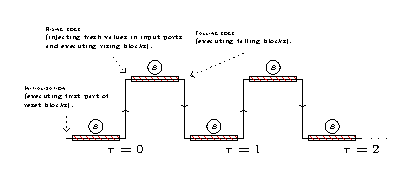
\includegraphics[keepaspectratio,width=\textwidth]{sim-alg.eps}
  \caption{The simulation algorithm as defined for \hvhdl{}
    designs. The hatched areas indicate a stabilization phase
    happening between two clock edges. }
  \label{fig:sim-alg}
\end{figure}

Figure~\ref{fig:sim-alg} illustrates the different phases of the
\hvhdl{} simulation algorithm, each triggering the execution of
specific parts of the design under simulation. The different phases of
the algorithm are tied to the events of a synchronization signal
(i.e. a clock signal). At the beginning of the simulation, the
initialization phase triggers the execution of the first part of reset
blocks, and a stabilization phase follows. Then, the same phases are
repeated over each clock cycle of the simulation:

\begin{enumerate}
\item At the start of each clock cycle, fresh values are injected in
  the input ports of the design under simulation, referred to as
  \textit{primary} input ports.
\item At the occurrence of the rising (resp. falling) edge of the
  clock signal, all rising (resp. falling) edge blocks are executed
  and a stabilization phase follows.  
\end{enumerate}

Our aim is to simplify as much as possible our formal setting to ease
the proof of semantic preservation and its mechanization. Simplifying
as much as possible the simulation algorithm will lead to
straight-forward reasoning at the time of proofs, whereas the
formalization of fully-fledged simulation algorithm, however not
deprived of interests (e.g. to set the formal specification of a
\vhdl{} simulator), will only contribute to add complexity to our
proofs.

\paragraph{Stabilization}

During a stabilization phase, all the combinational parts of a
design's behavior are executed. In the \hvhdl{} language, all
statements that are not enclosed in falling or rising blocks are
considered as combinational statements (with the exception of the
first part of reset blocks), and are thus executed during the
stabilization phase. In Table~\ref{tab:stabilization}, we define the
stabilization phase through a stabilization relation written
$\mathcal{D},\Delta,\sigma\vdash{}cs\xrightarrow{\rightsquigarrow}\sigma'$,
where $\mathcal{D}\in{}id\nrightarrow{}design$ is a design store,
$\Delta\in{}ElDesign$ is the elaborated version of the design being
simulated, $\sigma\in{}\Sigma$ is the design state at the beginning of
the stabilization phase, $cs$ is a concurrent statement representing
the behavior of the design being simulated, and $\sigma'\in\Sigma$ is
the design state at the end of the stabilization phase.

\begin{table}[!h]
  \caption{Evaluation of a \hvhdl{} design's behavior during a
    stabilization phase.}
  \label{tab:stabilization}
  
  \begin{tabular}{@{}l}
    % {\fontsize{10}{13}\selectfont\textsc{StabilizeEnd}} \\    
    {\begin{prooftree}[template=\inserttext]

        \hypo{$\mathcal{D},\Delta,\sigma\vdash{}cs\xrightarrow{cs_c}\sigma'$}
        \infer1[$\sigma\stackrel{\Sigma}{=}\sigma'$]
        {
          $\mathcal{D},\Delta,\sigma\vdash{}cs\xrightarrow{\rightsquigarrow}\sigma'$
        }
      \end{prooftree}} \\
  \end{tabular}
  \begin{tabular}{l}
    % {\fontsize{10}{13}\selectfont\textsc{StabilizeLoop}} \\
    {\begin{prooftree}[template=\inserttext]
        \hypo{$\mathcal{D},\Delta,\sigma\vdash{}cs\xrightarrow{cs_c}\sigma'$}
        \hypo{$\mathcal{D},\Delta,\sigma'\vdash{}cs\xrightarrow{\rightsquigarrow}\sigma''$}
        \infer2[$\sigma\stackrel{\Sigma}{\neq}\sigma'$]
        {
          $\mathcal{D},\Delta,\sigma\vdash{}cs\xrightarrow{\rightsquigarrow}\sigma''$
        }
      \end{prooftree}} \\
  \end{tabular}
\end{table}

As expressed in Table~\ref{tab:stabilization}, if after the execution
of $cs$ the starting state and the resulting state are equal (i.e. the
evaluation of the behavior does no longer affect the value of signals
or design instance states) regarding the state equality relation
written $\stackrel{\Sigma}{=}$, then a stable state has been reached
and the stabilization phase ends.  Otherwise, the behavior is executed
with the resulting state as input until a stable state is
reached. Note that in the presence of combinational loops (i.e. when a
signal that is the target of an assignment operation refers to its own
value in the right part of the assignment), the execution of a
design's behavior possibly leads to an infinite loop.

The state equality relation, used to determine if a stable state has
been reached, is inductively defined as follows: two states
$\sigma,\sigma'\in{}\Sigma$ are \textit{state}-equal, written
$\sigma\stackrel{\Sigma}{=}\sigma'$, if the value of the signals
referenced in their signal store are equal, and if the state of all
design instances referenced in their design instance store are
state-equal. Namely:
$\sigma\stackrel{\Sigma}{=}\sigma'\equiv
\big(\forall{}id_s,~\mathcal{S}(\sigma)(id_s)=\mathcal{S}(\sigma')(id_s)\big)
\land\big(\forall{}id_c,~\mathcal{C}(\sigma)(id_c)\stackrel{\Sigma}{=}\mathcal{C}(\sigma')(id_c)\big)$\footnote{We
  assume that both the domains of the signal stores and of the design
  instance stores of $\sigma$ and $\sigma'$ are equal.}.

% \begin{table}[!h]

%   \caption{Evaluation of a \hvhdl{} design's behavior during the
%     initialization phase.}
%   \label{tab:init}
  
%   % {\fontsize{10}{13}\selectfont\textsc{Init}}
%   \begin{prooftree}[template=\inserttext]

%     % Run all processes once.
%     \hypo{$\mathcal{D},\Delta,\sigma\vdash\mathrm{cs}\xrightarrow{cs_i}{}\sigma'$}

%     % Stabilization phase after runinit.
%     \hypo{$\mathcal{D},\Delta,\sigma'\vdash\mathrm{cs}\xrightarrow{\rightsquigarrow}{}\sigma_0$}

%     % Conclusion.
%     \infer2
%     {
%       $\mathcal{D},\Delta,\sigma\vdash\mathrm{cs}\xrightarrow{init}\sigma_0$
%     }

%   \end{prooftree}
% \end{table}

\paragraph{Main loop and full simulation}



The rules of Table~\ref{tab:sim-loop} define the \hvhdl{} simulation
relation which is a relational definition of our simulation algorithm
given in a structural \textit{small-step} setting (i.e. all
intermediary states are preserved in a simulation trace).  The
simulation relation is written
$\mathcal{D},E_p,\Delta,\tau,\sigma\vdash{}cs\rightarrow\theta$. It
associates the execution of a behavior $cs$ with a simulation trace
$\theta\in\mathtt{list}(\Sigma)$ in a context
$\mathcal{D},E_p,\Delta,\tau,\sigma$ where
$\mathcal{D}\in{}id\nrightarrow{}design$ is a design store,
$E_p\in\mathbb{N}\rightarrow(id\nrightarrow{}v)$ is a simulation
environment that will be used to update the value of primary input
ports at the beginning of each simulation cycle, $\Delta\in{}ElDesign$
is the elaborated version of the design under simulation, $\tau$ is
the number of clock cycles to be performed during the simulation, and
$\sigma$ is the design state at the beginning of the simulation. The
simulation trace $\theta$, which is a list of time-ordered design
states, is the result of the execution of the design behavior $cs$
during $\tau$ clock cycles. Here, $cs$ represents the behavior of the
\hvhdl{} design under simulation.

\begin{table}[!h]
  \caption{Simulation main loop}
  \label{tab:sim-loop}
  
    \begin{tabular}{l}
    % SIMULATION LOOP
    % {\fontsize{10}{13}\selectfont\textsc{SimLoop}} \\
    
    {\begin{prooftree}[template=\inserttext]
        
        % First column.
        % Rising
        \hypo{$\mathcal{D},\Delta,\mathtt{inj}(\sigma,E_p,\tau)\vdash{}cs\xrightarrow{cs_\uparrow}\sigma_\uparrow$}

        % Stabilize after rising.
        \infer[no rule]1{$\mathcal{D},\Delta,\sigma_\uparrow\vdash{}cs\xrightarrow{\rightsquigarrow}\sigma'$}

        % Falling
        \infer[no rule]1{$\mathcal{D},\Delta,\sigma'\vdash{}cs\xrightarrow{cs_\downarrow}\sigma_\downarrow$}
        
        % Stabilize after falling.
        \infer[no rule]1{$\mathcal{D},\Delta,\sigma_\downarrow\vdash{}cs\xrightarrow{\rightsquigarrow}\sigma''$}

        % Second column.
        \hypo{$\mathcal{D},E_p,\Delta,\tau-1,\sigma''\vdash{}cs\rightarrow\theta$}
        
        \infer2 [$\tau>0$] {
          $\mathcal{D},E_p,\Delta,\tau,\sigma\vdash{}cs\rightarrow(\sigma'
          :: \sigma'' :: \theta)$ }
      \end{prooftree}} \\
  \end{tabular}

  \vspace{10pt}
  
  \begin{tabular}{l}
    %%% SIMULATION END.
    
    % {\fontsize{10}{13}\selectfont\textsc{SimEnd}} \\
    
    {\begin{prooftree}[template=\inserttext]
        \infer0 {
          $\mathcal{D},E_p,\Delta,0,\sigma\vdash{}cs\rightarrow{}[~]$
        }
      \end{prooftree}} \\
  \end{tabular}
\end{table}


As shown in Table~\ref{tab:sim-loop}, the \hvhdl{} simulation relation
is defined through two rule instances.  In the case where $\tau$ is
equal to zero, the simulation ends and the execution of $cs$ returns
an empty trace. In the case where $\tau$ is greater than zero, one
simulation cycle is performed with $\sigma$ as the starting state. At
the beginning of the cycle, the value of the input ports of the design
under simulation are updated with the values yielded by the simulation
environment $E_p$ at clock count $\tau$. Given a simulation
environment $E_p\in\mathbb{N}\rightarrow(id\nrightarrow{}v)$, the
\texttt{inj} function that updates the value of signals at a given
design state $\sigma\in\Sigma$ and clock cycle count
$\tau\in{}\mathbb{N}$ is defined as follows:
$\mathtt{inj}(\sigma,E_p,\tau)=(\mathcal{S}_i,\mathcal{C})$ where
$\sigma=(\mathcal{S},\mathcal{C}), $ and $\mathcal{S}_i(x)=
\begin{cases}
  E_p(\tau)(x) & \mathrm{if}~x\in\mathtt{dom}(E_p(\tau)) \\
  \mathcal{S}(x) & \mathrm{otherwise}
\end{cases}$.

After the update of the input ports, the following sequence performs
the different phases of a clock cycle. First, all rising blocks
defined in the behavior of the design under simulation are
executed. The rising blocks correspond to the part of the design
behavior that are sensitive to the rising edge event of the clock
signal. % Remember that a \hvhdl{} design represents a synchronous
% design, meaning that its execution is synchronized with a clock
% signal.
The $\uparrow$ flag is appended to the evaluation relation for
concurrent statements to execute rising blocks. Then, follows a
stabilization phase that produces a stable state $\sigma'$. After
that, the falling blocks are executed in response to the occurrence of
the falling edge event of the clock signal. Another stabilization
phase follows that produces a stable state $\sigma''$.  Then, the
\hvhdl{} simulation relation calls itself recursively with a
decremented cycle count and with state $\sigma''$ as the new starting
state. The recursive call yields a trace $\theta$ which is appended to
the states $\sigma'$ and $\sigma''$ to form the final simulation
trace. Note that we preserve in the simulation trace only stable
states, i.e. states at half a clock cycle and states at the end of a
clock cycle both resulting from a stabilization phase.

Table~\ref{tab:full-sim} presents the relation that formalizes our
entire simulation algorithm by appealing to the elaboration relation,
and to the simulation relation presented in
Table~\ref{tab:sim-loop}. The full simulation relation states that the
simulation of a design $d$ during $\tau$ clock cycles yields the trace
$(\sigma_0::\theta)$ in the context of the design store
$\mathcal{D}\in{}id\nrightarrow{}design$, the dimensioning function
$\mathcal{M}_g\in{}id\nrightarrow{}v$ (used for the elaboration of
design $d$), and under the simulation environment
$E_p\in\mathbb{N}\rightarrow(id\nrightarrow{}v)$. Here $\sigma_0$
represents the \textit{initial state} of the design. The initial state
is computed through an initialization phase consisting of the
execution of the first part of reset blocks (the $i$ flag is on)
followed by a stabilization phase. The execution of reset blocks
corresponds to the virtual activation of a reset signal at the
beginning of the simulation. This reset signal triggers the execution
of specific parts of the behavior responsible for the initialization
of the value of chosen signals, which are all associated to an
implicit default value otherwise\footnote{In the default state,
  i.e. the state yielded after the elaboration of a design, all
  signals are associated to the implicit default value of their type
  in the signal store. }. Then, the simulation trace $\theta$ is the
result of the simulation of design $d$ during $\tau$ clock cycles with
$\sigma_0$ as starting state. As a side condition, we enforce the fact
that, at every clock count of the simulation, the definition domain of
the simulation environment is a subset of the input port
identifiers. Otherwise, the update of signal values happening at the
beginning of a clock cycle possibly overrides the value of signals
other than input ports.

\begin{table}[!h]

  \caption{Full simulation}
  \label{tab:full-sim}
  % {\fontsize{10}{13}\selectfont\textsc{FullSim}}
  
  \begin{prooftree}[template=\inserttext]

    % Design elab.
    \hypo{$\mathcal{D},\mathcal{M}_g\vdash{}d\xrightarrow{elab}\Delta,\sigma$}

    % Initialization.
    
    % Run all processes once.
    \hypo{$\mathcal{D},\Delta,\sigma\vdash{}d.beh\xrightarrow{cs_i}{}\sigma'$}

    % Stabilization phase after init.
    \infer[no rule]1{$\mathcal{D},\Delta,\sigma'\vdash{}d.beh\xrightarrow{\rightsquigarrow}{}\sigma_0$}
    
    % Simulation main loop.
    \infer[no rule]1{$\mathcal{D},E_p,\Delta,\tau,\sigma_0\vdash{}{}d.beh\rightarrow\theta$}
    
    \infer2 [$\forall\tau_i\in\mathbb{N},~\mathsf{dom}(E_p)(\tau_i)\subseteq{}\mathsf{dom}(I(\Delta))$] { $\mathcal{D},\mathcal{M}_g,E_p,\tau\vdash$
      ${}d\xrightarrow{full}(\sigma_0::\theta)$ }
  \end{prooftree}
\end{table}

\section{Model-to-text transformation}
\label{sec:m2t}

In the following section, we present the \hilecop{} model-to-text
transformation (HM2T) through its formal specification. The goal of
the transformation is to generate a \hvhdl{} design that implements an
input SITPN model. To obtain an output design with the same behavior
than the input model, the execution semantics of SITPNs must be
encoded in terms of \vhdl{} code. To achieve this, the place and the
transition designs have been defined. The behavior of these two
designs, given in Appendices~\ref{app:place-design} and
\ref{app:trans-design}, correspond to a place-centered and
transition-centered implementation of the SITPN semantics in
\vhdl{}. At the moment of the transformation, instances of the place
and the transition designs, referred to as PDIs and TDIs, will be
created for each place and transition of the input model. Then, these
subcomponents of the output design's behavior will be interconnected
through their port interface.  While the SITPN execution semantics is
scattered in the internal behavior of PDIs and TDIs, the
interconnection of these instances permits us to obtain the global
behavior of the input model at runtime (or at least, that is what we
want to prove). Moreover, the interpretation elements of the input
SITPN model, namely the conditions, actions and functions will be
implemented by the input and output ports of the output design. The
conditions will be translated into Boolean input ports (referred to as
condition ports) in the generated design. The transition-condition
associations will be implemented by the interconnections between
condition ports and the interface of transition design instances
(TDIs). The activation/execution status of actions/functions will be
reflected by the value of the Boolean output ports (referred to as
action and function ports) of the generated design. The transformation
will generate two processes, namely the \texttt{actions} and
\texttt{functions} processes, that will be responsible for the
assignment of values to the action and function ports.

There exists a mapping between the elements of the input SITPN model
and their corresponding version in the generated \hvhdl{} design. This
mapping is captured within a structure called a SITPN-to-\hvhdl{}
binder.  This structure is generated alongside the transformation of
the input SITPN model into a \hvhdl{} design. It is both useful to
implement the HM2T as a program and to express its formal
specification. Definition~\ref{def:sitpn-to-hvhdl-binder} formally
describes the SITPN-to-\hvhdl{} binder structure:
\begin{definition}[SITPN-to-\hvhdl{} design binder]
  \label{def:sitpn-to-hvhdl-binder}
  Given a $sitpn\in{}SITPN$ and a \hvhdl{} design $d\in{}design$, a
  SITPN-to-\hvhdl{} binder $\gamma\in{}WM(sitpn,d)$ is a record
  ${<}PMap,TMap,CMap,AFMap{>}$ where:
  \begin{itemize}
  \item $PMap\in{}P\rightarrow{}\{id_p~|~\mathtt{comp}(id_p,\mathtt{place},g,i,o)\in{}d.beh\}$
  \item $TMap\in{}T\rightarrow{}\{id_t~|~\mathtt{comp}(id_t,\mathtt{transition},g,i,o)\in{}d.beh\}$
  \item $CMap\in\mathcal{C}\rightarrow\{id_c~|~(\mathtt{in}, id_c, \mathtt{bool})\in{}d.ports\}$
  \item $AFMap\in\mathcal{A}\cup\mathcal{F}\rightarrow\{id_{af}~|~(\mathtt{out}, id_{af}, \mathtt{bool})\in{}d.ports\}$
  \end{itemize}
\end{definition}

For a given binder $\gamma$ and an element of an SITPN structure
$e\in{}P\cup{}T\cup\mathcal{C}\cup\mathcal{A}\cup\mathcal{F}$, we
write $\gamma(e)$ where $e$ is looked up in the appropriate
function. For instance, for a given $f\in\mathcal{F}$, $\gamma(f)$ is
a shorthand notation for $AFMap(f)$ where $\gamma={<}\dots,AFMap{>}$.

\bigskip

The formal specification of the HM2T is expressed as a relation
between the inputs of the transformation, namely a SITPN model and a
bounding function, and its outputs, which can be either a pair
composed of a \hvhdl{} design and a SITPN-to-\hvhdl{} binder or the
error value. The relation is written
$HM2T_{\mathtt{spec}}\subseteq{}SITPN\times(P\rightarrow\mathbb{N})\times{}((design\times{}WM(sitpn,d))\cup\{\mathtt{err}\})$
where $sitpn$ and $d$ refer to the first and the third parameters of
the relation. As hinted at the beginning of the section, specifying
the HM2T is mostly about describing how the PDIs and TDIs are
interconnected through their port interface. The error case arises
when the input SITPN model does not respect the well-definition
property (cf. Definition~\ref{def:wd-sitpn}).

The bounding function, that is, the second parameter of the
$HM2T_{\mathtt{spec}}$ relation, associates each place of the SITPN
model with a bound in terms of number of tokens.  A bound represents
the maximum number of tokens that a place will possibly hold at some
point of the execution of the model. We assume that these bounds have
been computed through the formal analysis of the input SITPN model. Of
course, the existence of such a function implies that all the SITPN
models that are passed as inputs to the HM2T are \textit{bounded}
models\footnote{There exists no place that can accumulate an unlimited
  number of tokens in the course of the execution of the model.}. As a
matter of fact, we can prove that the HM2T is not semantic-preserving
when the input is an unbounded SITPN model. The execution of such a
model will lead to an infinite incrementation of the number of tokens
in a given place. This infinite incrementation, while valid in the
mathematical world, can never be mirrored by a \vhdl{} implementation
of the model where all values must be finite. Therefore, the behavior
of the SITPN model and its \hvhdl{} implementation will diverge at
some point of their execution.

\bigskip

Definition~\ref{def:hm2t-spec} presents the formal specification of
the HM2T through a selected set of points. The full definition of the
HM2T's formal specification can be found in
\cite{Iampietro2022hfspec}. Each point of the definition will be
commented and illustrated as and when they arise. We have implemented
the $HM2T_{\mathtt{spec}}$ relation in \coq{}, and have written a
\coq{} function, named \texttt{sitpn2hvhdl}, that implements the
transformation but is yet to be proved sound and complete regarding
its specification. In Definition~\ref{def:hm2t-spec}, we also refer to
the names of generic constants and signals declared in the place and
transition designs. To achieve conciseness, we use aliases to refer to
these constants and signals. The correspondence between the aliases
and the full names is given in Appendix~\ref{sec:cnsts-sigs-names}.

%%%%% Definition for the HM2T formal specification. %%%%%

\def\pdiInBeh{\mathtt{comp}(\gamma(p),\mathtt{place},g_p,i_p,o_p)\in{}d.beh}
\def\tdiInBeh{\mathtt{comp}(\gamma(t),\mathtt{transition},g_t,i_t,o_t)\in{}d.beh}
\def\tdiInBehP#1{\mathtt{comp}(\gamma(#1),\mathtt{transition},g_{#1},i_{#1},o_{#1})\in{}d.beh}

\begin{definition}[\hilecop{} model-to-text transformation specification]
  \label{def:hm2t-spec}
  For all SITPN model $sitpn\in{}SITPN$, bounding function
  $b\in{}P\rightarrow\mathbb{N}$, \hvhdl{} design $d\in{}design$, and
  SITPN-to-\hvhdl{} binder $\gamma\in{}WM(sitpn,d)$, we have
  $HM2T_{\mathtt{spec}}(sitpn,b,(d,\gamma))$ if:
  \begin{enumerate}
  \item\label{it:pdi-tdi-only} All design instantiation statement in
    the design's behavior
    either creates a PDI or a TDI: \\
    $\forall{}id_c,id_e,g,i,o~s.t.~\mathtt{comp}(id_c,id_e,g,i,o)\in{}d.beh,~id_e=\mathtt{place}\lor{}id_e=\mathtt{transition}$.
    
  \item\label{it:actions-functions-only} The \texttt{actions} and
    \texttt{functions} processes are the
    only two processes in the design's behavior:\\
    $\forall{}id_p,vars,ss~s.t.~\mathtt{ps}(id_p,vars,ss)\in{}d.beh,~id_p=\mathtt{actions}\lor{}id_p=\mathtt{functions}$.
    
  \item\label{it:d-is-elaborable} Design $d$ is elaborable in the context of the \hilecop{} design store\footnote{The \hilecop{} design store is a specific design store that holds the definition of the \texttt{place} and \texttt{transition} designs.} and given an empty dimensioning function:\\
    $\exists{}\Delta\in{}ElDesign,\sigma_e\in\Sigma$ s.t.
    $\mathcal{D_\mathcal{H}},\emptyset\vdash{}d\xrightarrow{elab}\Delta,\sigma_e$.
    
  \item\label{it:binder-bij} All the fields of the SITPN-to-\hvhdl{} binder are bijective
    functions: $PMap(\gamma)$ is bijective, $TMap(\gamma)$ is
    bijective,\dots
  \end{enumerate}

  \bigskip
  
  Points~\ref{it:pdi-tdi-only} to \ref{it:binder-bij} specify the
  global shape of the output design $d$ and the binder structure
  $\gamma$.  Point~\ref{it:pdi-tdi-only} states that the behavior of
  design $d$ is only composed of place or transition design
  instances. Point~\ref{it:actions-functions-only} states that there
  are only two processes in the behavior of the output design, namely
  the $\mathtt{actions}$ process and the $\mathtt{functions}$
  process. The content of the \texttt{actions} process is specified in
  Point~\ref{it:actions}. Point~\ref{it:d-is-elaborable} states that
  the output design is elaborable, i.e. syntactically well-formed,
  statically well-typed, with no multiply-driven signals, etc.
  Point~\ref{it:binder-bij} states that there is a one-to-one
  correspondence between the elements of the input SITPN model and the
  elements of the output design and that this correspondence is
  established through the binder $\gamma$.

  \bigskip
  
  \begin{enumerate}[resume]
  \item\label{it:pdi-exists} For all place of the input SITPN model,
    there exists a corresponding PDI identified through $\gamma$ in
    the behavior of the output
    design:\\
    $\forall{}p\in{}P,\exists{}g_p,i_p,o_p$ s.t.  $\pdiInBeh$.
    
  \item\label{it:pdi-gmap} For all place of the input SITPN model and
    its corresponding PDI, the generic map of the PDI holds the
    following associations:
    \begin{equation*}
      \begin{aligned}
        \forall{}p\in&{}P,g_p,i_p,o_p, \\
        & \pdiInBeh\Rightarrow \\
        &
          \begin{aligned}
            g_p=\{&(\mathtt{mm}\Rightarrow{}b(p)), \\
                  & (\mathtt{ian}\Rightarrow
                    \begin{cases}
                      1~\mathrm{if}~\mathtt{input}(p)=\emptyset \\
                      \vert{}\mathtt{input}(p)\vert~\mathrm{otherwise} \\
                    \end{cases}), \\
                  &(\mathtt{oan}\Rightarrow
                    \begin{cases}
                      1~\mathrm{if}~\mathtt{output}(p)=\emptyset \\
                      \vert{}\mathtt{output}(p)\vert~\mathrm{otherwise} \\
                    \end{cases})\} \\
          \end{aligned} \\
      \end{aligned}
    \end{equation*}
    where
    \texttt{input}$(p)=\{t~\vert~post(t,p)=\lfloor\omega\rfloor\}$,
    the set of input transitions of place $p$, and
    \texttt{output}$(p)=\{t~\vert~pre(p,t)=\lfloor(\omega,a)\rfloor\}$,
    the set of output transitions of place $p$.
    
  \item\label{it:pdi-im} For all place of the input SITPN model and
    its corresponding PDI, there is an association between the
    \texttt{im} input port and the initial marking of the place in the
    input port map of the PDI:\\
    $\forall{}p\in{}P,g_p,i_p,o_p,\pdiInBeh{}$
    $\Rightarrow(\mathtt{im}\Rightarrow{}M_0(p))\in{}i_p$.
  \end{enumerate}

  \bigskip

  Point~\ref{it:pdi-exists} states the existence of a corresponding
  PDI in the behavior of the output design for each place of the input
  SITPN model. Point~\ref{it:pdi-gmap} describes how the content of
  the generic map of a PDI is computed based on the properties of the
  corresponding place. Note that the \texttt{mm} constant,
  corresponding to the maximal marking of the PDI, receives its value
  from the bounding function. Point~\ref{it:pdi-im} describes how the
  initial marking of the place is reflected on the input port map of
  the corresponding PDI through the \texttt{im} input
  port. Figure~\ref{fig:gen-pci-ex} illustrates the link between the
  number of input and output arcs of a place and how this information
  is passed through the generic map and impacts the dimensioning of
  the corresponding PDI's port interface.

  \begin{figure}[h]
    \centering
    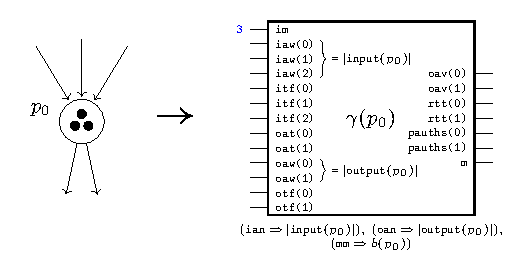
\includegraphics[keepaspectratio,width=.7\textwidth]{gen-pci-ex.eps}
    \caption{A graphical representation of the interface of the PDI
      $\gamma(p_0)$ (on the right) implementing place $p_0$ (on the
      left). The generic map associations appear underneath the PDI.}
    \label{fig:gen-pci-ex}
  \end{figure}
  
  \begin{enumerate}[resume]

  \item\label{it:exists-tdi} For all transition of the input SITPN model, there exists a
    corresponding TDI identified through $\gamma$ in the behavior of
    the output design:\\
    $\forall{}t\in{}T,\exists{}g_t,i_t,o_t$ s.t. $\tdiInBeh$.
    
  \item\label{it:tdi-gen-map} For all transition of the input SITPN model and its
    corresponding TDI, the generic map of the TDI holds the following
    associations:
    \begin{equation*}
      \begin{aligned}[t]
        \forall{}t&\in{}T,g_t,i_t,o_t, \\
                  & \tdiInBeh\Rightarrow \\
                  &
                    \begin{aligned}[t]
                      g_t=\{&(\mathtt{tt}\Rightarrow{}
                      \begin{cases}
                        \mathtt{not\_temp}~\mathrm{if}~t\notin{}\mathtt{dom}(I_s) \\
                        \mathtt{temp\_a\_a}~\mathrm{if}~I_s(t)=[a,a] \\
                        \mathtt{temp\_a\_b}~\mathrm{if}~I_s(t)=[a,b] \\
                        \mathtt{temp\_a\_inf}~\mathrm{if}~I_s(t)=[a,\infty] \\
                      \end{cases}),\\
                      & (\mathtt{mtc}\Rightarrow
                      \begin{cases}
                        1~\mathrm{if}~t\notin{}\mathtt{dom}(I_s) \\
                        b~\mathrm{if}~I_s(t)=[a,b] \\
                        a~\mathrm{if}~I_s(t)=[a,\infty] \\
                      \end{cases}), \\
                      & (\mathtt{ian}\Rightarrow
                        \begin{cases}
                          1~\mathrm{if}~\mathtt{input}(t)=\emptyset \\
                          \vert{}\mathtt{input}(t)\vert~\mathrm{otherwise} \\
                        \end{cases}), 
                      (\mathtt{cn}\Rightarrow
                      \begin{cases}
                        1~\mathrm{if}~\mathtt{conds}(t)=\emptyset \\
                        \vert{}\mathtt{conds}(t)\vert~\mathrm{otherwise} \\
                      \end{cases})\}. \\
                    \end{aligned} \\
      \end{aligned}
    \end{equation*}
    where
    \texttt{input}$(t)=\{p~\vert~pre(p,t)=\lfloor(\omega,a)\rfloor\}$,
    the set of input places of transition $t$, and
    \texttt{conds}$(t)=\{c~\vert~\mathbb{C}(t,c)=1\lor\mathbb{C}(t,c)=-1\}$,
    the set of conditions associated with transition $t$.
    
  \item\label{it:tdi-time-itval} For all transition of the input SITPN
    model and its corresponding TDI, the input port map of the TDI
    holds the following associations:
    \begin{equation*}
      \begin{aligned}[t]
        \forall{}t&\in{}T,g_t,i_t,o_t, \\
                  & \tdiInBeh\Rightarrow \\
                  &
                    \begin{aligned}[t]
                      \{&(\mathtt{A}\Rightarrow\begin{cases}
                                                0~\mathrm{if}~t\notin\mathtt{dom}(I_s) \\
                                                l(I_s(t))~\mathrm{otherwise} \\
                                              \end{cases}), \\
                      & (\mathtt{B}\Rightarrow\begin{cases}
                                              0~\mathrm{if}~t\notin\mathtt{dom}(I_s)\lor{}u(I_s(t))=\infty \\
                                              u(I_s(t))~\mathrm{otherwise} \\
                                            \end{cases})\}\subseteq{}i_t. \\
                    \end{aligned}
        \\
      \end{aligned}
    \end{equation*}

  \end{enumerate}

  \bigskip

  Similarly to the case of places, Points~\ref{it:exists-tdi} to
  \ref{it:tdi-time-itval} state the existence of a corresponding TDI
  for each transition of the input model, and specify how its generic
  map and its input port map must be built regarding the properties of
  the transition, namely: the type of the time interval, the number of
  input arcs, the number of associated
  conditions. Figure~\ref{fig:gen-tdi-ex} illustrates how the
  properties of a transition are implemented in the interface of the
  corresponding TDI.

  \begin{figure}[h]
    \centering
    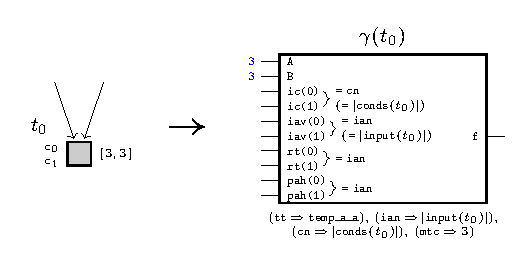
\includegraphics[keepaspectratio,width=.8\textwidth]{gen-tdi-ex.eps}
    \caption{A graphical representation of the interface of the TDI
      $\gamma(t_0)$ (on the right) implementing transition $t_0$ (on
      the left). The generic map associations appear underneath the
      TDI.}
    \label{fig:gen-tdi-ex}
  \end{figure}
  
  \begin{enumerate}[resume]        
  \item\label{it:post-arc} For all post arc of the input SITPN model,
    the TDI and PDI corresponding to the source transition and target
    place of the arc are connected as follows:
    \begin{equation*}
      \begin{aligned}[t]
        \forall{}t&\in{}T,p\in{}P,g_t,i_t,o_t,g_p,i_p,o_p,\omega\in\mathbb{N}^{*}, \\
                  & post(t,p)=\lfloor\omega\rfloor\Rightarrow \\
                  & \tdiInBeh\Rightarrow \\
                  & \pdiInBeh\Rightarrow\\
                  &
                    \begin{aligned}[t]
                      \exists{}i & \in[0,\vert\mathtt{input}(p)\vert-1]~s.t.~(\mathtt{iaw}(i)\Rightarrow\omega)\in{}i_p \\
                                 & \land\exists{}id_s~s.t.~(id_s,\mathtt{bool})\in{}d.sigs
                                   \land(\mathtt{fired}\Rightarrow{}id_s)\in{}o_t\land(\mathtt{itf}(i)\Rightarrow{}id_s)\in{}i_p. \\
                    \end{aligned}
        \\
      \end{aligned}
    \end{equation*}
  \end{enumerate}
  
  \bigskip

  In Point~\ref{it:post-arc}, $(id_s,\mathtt{bool})\in{}d.sigs$
  indicates the signal $id_s$ is declared as a Boolean internal signal
  in the output design. Figure~\ref{fig:gen-post-arc} illustrates the
  translation of a post arc of the input SITPN model as described in
  Point~\ref{it:post-arc}. The weight of the arc is passed to the PDI
  through the \texttt{iaw} (for \texttt{input\_arcs\_weights}) input
  port. In the behavior of the output design, all arc information is
  encoded through the input port interface of PDIs. All computations
  that necessitate the arc information, such as the marking update or
  the setting of time counter reset signals, are performed in the
  behavior of the place design. Therefore, only the PDIs need to hold
  the arc information.

  \begin{figure}[h]
    \centering
    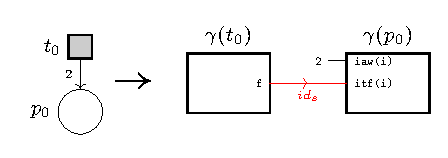
\includegraphics[keepaspectratio,width=.7\textwidth]{gen-post-arc.eps}
    \caption{The translation of a post arc, connecting a transition
      $t_0$ to a place $p_0$, into an interconnection between the
      interfaces of the corresponding TDI and PDI.}
    \label{fig:gen-post-arc}
  \end{figure}
  
  \begin{enumerate}[resume]
  \item\label{it:pre-arc} For all pre arc of the input SITPN model,
    the PDI and TDI corresponding to the source place and target
    transition of the arc are connected as follows:
    \begin{equation*}
      \begin{aligned}[t]
        \forall{}t&\in{}T,p\in{}P,g_t,i_t,o_t,g_p,i_p,o_p,\omega\in\mathbb{N}^{*},a\in\{\mathtt{basic},\mathtt{test},\mathtt{inhib}\}, \\
                  & pre(p,t)=\lfloor(\omega,a)\rfloor\Rightarrow \\
                  & \tdiInBeh\Rightarrow \\
                  & \pdiInBeh\Rightarrow\\
                  & \exists{}i\in[0,\vert\mathtt{output}(p)\vert-1]~s.t.~\{(\mathtt{oaw}(i)\Rightarrow\omega),(\mathtt{oat}(i)\Rightarrow{}a)\}\subseteq{}i_p \\
                  & \begin{aligned}[t]
                      \land\exists{}j &\in[0,\vert\mathtt{input}(t)\vert-1],id_{av},id_{rt},id_{frd},id_{pah}~s.t. \\
                                      & \{(id_{av},\mathtt{bool}),(id_{rt},\mathtt{bool}),(id_{frd},\mathtt{bool}),(id_{pah},\mathtt{bool})\}\subseteq{}d.sigs \\
                                      & \land(\mathtt{oav}(i)\Rightarrow{}id_{av})\in{}o_p\land(\mathtt{iav}(j)\Rightarrow{}id_{av})\in{}i_t \\
                                      & \land(\mathtt{rtt}(i)\Rightarrow{}id_{rt})\in{}o_p\land(\mathtt{rt}(j)\Rightarrow{}id_{rt})\in{}i_t \\
                                      & \land(\mathtt{otf}(i)\Rightarrow{}id_{frd})\in{}i_p\land(\mathtt{fired}\Rightarrow{}id_{frd})\in{}o_t \\
                                      & \land(\mathtt{pah}(i)\Rightarrow{}id_{frd})\in{}o_p \\
                                      & \land(a=\mathtt{test}\lor{}a=\mathtt{inhib}\lor{}\mathtt{sbmut}(p)\Rightarrow(\mathtt{pah}(j)\Rightarrow\mathtt{true})\in{}i_t) \\
                                      & \land(a=\mathtt{basic}\land{}\lnot\mathtt{sbmut}(p)\Rightarrow(\mathtt{pah}(j)\Rightarrow{}id_{pah})\in{}i_t). \\
                    \end{aligned} \\
      \end{aligned}
    \end{equation*}
    where $\mathtt{sbmut}(p)$ is a predicate stating that all
    conflicts in the output transitions of a given place $p$ are
    solved by mutual exclusion as outlined in
    Definition~\ref{def:mutex-conds} and \ref{def:mutex-inhib}.

    % $\mathtt{confl}\in{}P\rightarrow{}2^T\cup\{\mathtt{err}\}$
    % takes a place $p$ as input and yields either an error or an
    % ordered set of transitions computed as follows:
    % \begin{enumerate}
    % \item If all conflicts between the output transitions of $p$ are
    %   solved by mutual exclusion, or if the set of conflicting
    %   transitions of $p$ is a singleton, then $\mathtt{confl}$ returns
    %   an empty set.
    % \item Otherwise, the function tries to establish a total ordering
    %   over the set of conflicting transitions of $p$ w.r.t the firing
    %   priority relation:
    %   \begin{itemize}
    %   \item If no such ordering can be established (in that case, the
    %     firing priority relation is ill-formed, and the input SITPN is
    %     not well-defined), $\mathtt{confl}$ returns the \texttt{err}
    %     value.
    %   \item Otherwise, the function returns the set in a decreasing
    %     priority order.
    %   \end{itemize}
    % \end{enumerate}
    
  \end{enumerate}

  \bigskip
  
  Figure~\ref{fig:gen-pre-arc} illustrates the translation of a pre
  arc of the input SITPN model as described in Point~\ref{it:pre-arc}.
  As for the post arcs, the arc information is passed through the
  input port map of the PDI. As there are three possible types of pre
  arc, the \texttt{oat} (for \texttt{output\_arcs\_types}) input port
  receives the arc type information.  In Figure~\ref{fig:gen-pre-arc},
  we assume that there remain some conflicts not solved by mutual
  exclusion in the set of output transitions of place
  $p_0$. Otherwise, according to Point~\ref{it:pre-arc}, the
  interconnection between $\mathtt{pah(i)}$ and $\mathtt{pah(j)}$
  would not be effective.
  
  \begin{figure}[h]
    \centering
    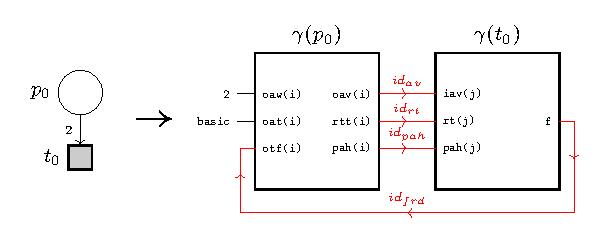
\includegraphics[keepaspectratio,width=.8\textwidth]{gen-pre-arc.eps}
    \caption{The translation of a pre arc, connecting a place $p_0$ to
      a transition $t_0$, into signal interconnections between the
      interfaces of the corresponding PDI and TDI. }
    \label{fig:gen-pre-arc}
  \end{figure}

  \begin{enumerate}[resume]
  \item\label{it:port-indices-ordering} For all place of the input
    SITPN model for which conflicts in its output transitions are not
    solved by mutual exclusion, the port indices of the corresponding
    PDI reflect the priority order established between the conflicting
    output transitions:
    \begin{equation*}
      \begin{aligned}[t]
        \forall{}p&\in{}P,t,t'\in{}\mathtt{confl}(p),g_p,i_p,o_p,g_t,i_t,o_t,g_{t'},i_{t'},o_{t'}, \\
                  & t\succ{}t'\Rightarrow\\
                  & \pdiInBeh\Rightarrow \\
                  & \tdiInBehP{t}\Rightarrow \\
                  & \tdiInBehP{t'}\Rightarrow \\
                  &
                    \begin{aligned}[t]
                      (\forall{}i,j&\in\mathbb{N},id_{frd},id_{frd'},id_{s},id_{s'},name_t,name_{t'},id_{out}, \\
                                   & (\mathtt{fired}\Rightarrow{}id_{frd})\in{}o_t\Rightarrow \\
                                   & (\mathtt{fired}\Rightarrow{}id_{frd'})\in{}o_{t'}\Rightarrow \\
                                   & \{(\mathtt{otf}(i)\Rightarrow{}id_{frd}),(\mathtt{otf}(j)\Rightarrow{}id_{frd'})\}\subseteq{}i_p\Rightarrow \\
                                   & (name_t\Rightarrow{}id_{s})\in{}i_t\Rightarrow \\
                                   & (name_{t'}\Rightarrow{}id_{s'})\in{}i_{t'}\Rightarrow \\
                                   & \{(id_{out}(i)\Rightarrow{}id_s),(id_{out}(j)\Rightarrow{}id_{s'})\}\subseteq{}o_p\Rightarrow \\
                                   & i<j) \\
                    \end{aligned} \\
      \end{aligned}
    \end{equation*}

    where
    \texttt{confl}$(p)=\{t~\vert~pre(p,t)=\lfloor(\omega,\mathtt{basic})\rfloor\}$,
    the set of conflicting output transitions of place $p$.
  \end{enumerate}

  \bigskip

  As specified in Point~\ref{it:port-indices-ordering}, the port
  indices in the interface of a PDI must reflect the priority order
  established between its \textit{conflicting} TDIs.%  Of course, this
  % is only mandatory for the ports connecting the PDI to its
  % conflicting TDIs. Otherwise, the index order does not matter, for
  % instance while reifying a post arc connection.
  Figure~\ref{fig:gen-prio-order} illustrates the ordering of the port
  indices in the interface of a PDI as described in
  Point~\ref{it:port-indices-ordering}.

  \begin{figure}[h]
    \centering
    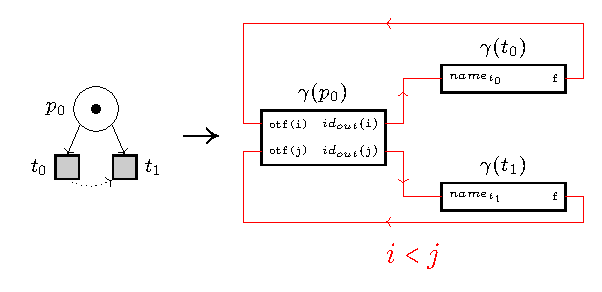
\includegraphics[keepaspectratio,width=.8\textwidth]{gen-prio-order.eps}
    \caption{Translation of the priority relation in terms of port
      index ordering. On the right, $name_{t_0}$ (resp. $name_{t_1}$)
      refers to any input port of TDI $\gamma(t_0)$
      (resp. $\gamma(t_1)$), and $id_{out}$ refers to any composite
      output port of PDI $\gamma(p_0)$. On the left, the dotted arc
      going from transition $t_0$ to $t_1$ indicates the $t_0$ has a
      higher firing priority than $t_1$. }
    \label{fig:gen-prio-order}
  \end{figure}

  \begin{enumerate}[resume]
  \item\label{it:actions} There exists an \texttt{actions} process
    that assigns a value to the output ports (referred to as
    \textit{action} ports) representing the activation status of the
    actions of the input SITPN model:
    
    $\exists{}ss_{ra},ss_{a}~s.t.~\mathtt{ps}(\mathtt{actions},\emptyset,\mathtt{rst}\{ss_{ra}\}\mathtt{else}\{\mathtt{falling}\{ss_a\}\})\in{}d.beh$
    and
    \begin{enumerate}
    \item The length of the $ss_{ra}$ and $ss_{a}$ sequences is equal
      to the number of actions of the input SITPN model:\\
      $\vert{}ss_{ra}\vert_{;}=\vert{}ss_a\vert_{;}=\vert\mathcal{A}\vert$
      where $\vert{}ss\vert{}_{;}=
      \begin{cases}
        \vert{}ss_1\vert_{;}+\vert{}ss_2\vert_{;}~\mathrm{if}~ss=ss_1;ss_2 \\
        1~\mathrm{otherwise}
      \end{cases}
      $
      
    \item During the initialization, all action ports are assigned to
      \texttt{false} by the \texttt{actions} process:
      $\forall{}a\in\mathcal{A},~\gamma(a)\Leftarrow\mathtt{false}\in{}ss_{ra}$
      
    \item An action port corresponding to an unassociated action is
      assigned to \texttt{false} during the falling edge
      phase:\\
      $\forall{}a\in\mathcal{A}~s.t.~\mathtt{pls}(a)=\emptyset,\gamma(a)\Leftarrow\mathtt{false}\in{}ss_{a}$
      where
      \texttt{pls}$(a)=\{p~\vert~\mathbb{A}(p,a)=\mathtt{true}\}$, the
      set of places associated with action $a$.
      
    \item Otherwise, the value of the action port is the result of the
      Boolean sum between the \texttt{marked} output port of all PDIs
      representing the places associated with the corresponding
      action:
      \begin{equation*}
        \begin{aligned}[t]
          \forall{}a&\in\mathcal{A},~\mathtt{pls}(a)\neq\emptyset\Rightarrow \\
                    &  \begin{aligned}[t]
                         \exists{}e_{or}& ~s.t.~\gamma(a)\Leftarrow{}e_{or}\in{}ss_a\land\mathtt{is\_bsum}(e_{or},\vert{}\mathtt{pls}(a)\vert) \\
                                        &
                                          \begin{aligned}
                                            \land\forall{}p& \in\mathtt{pls}(a),g_p,i_p,o_p, \\
                                                           & \pdiInBeh\Rightarrow \\
                                                           &
                                                             \begin{aligned}
                                                               \exists{}id_m& ~s.t.~(id_m,\mathtt{bool})\in{}d.sigs \\
                                                                            &\land{}id_m\in{}e_{or} \\
                                                                            & \land(\mathtt{marked}\Rightarrow{}id_m)\in{}o_p \\
                                                             \end{aligned} \\
                                          \end{aligned} \\
                       \end{aligned} \\
        \end{aligned}
      \end{equation*}
      where $\mathtt{is\_bsum}$ is defined as follows:

      \vspace{10pt}
      
      \begin{tabular}{l}
        {\begin{prooftree}
            \hypo{e\in{}\{id,b\}}
            \infer1{\mathtt{is\_bsum}(e,1)}
          \end{prooftree}} \\
      \end{tabular}
      \begin{tabular}{l}
        {\begin{prooftree}
            \hypo{\mathtt{is\_bsum}(e_1,n)}
            \hypo{\mathtt{is\_bsum}(e_2,m)}
            \infer2
            {\mathtt{is\_bsum}(\mathtt{or}(e_1,e_2),n+m)}
          \end{prooftree}} \\
      \end{tabular}
    \end{enumerate}
  \end{enumerate}

  \bigskip

  In Point~\ref{it:actions}, the $\mathtt{is\_bsum}$ relation states
  that a given expression is a Boolean sum (i.e. a composition of
  \texttt{or} expressions) of Boolean terminals or identifiers and
  that this expression has a given size. Through the \texttt{is\_bsum}
  relation, we want specify that all the internal signals connected to
  the \texttt{marked} ports of the associated PDIs are represented in
  the $e_{or}$ expression.  Figure~\ref{fig:gen-actions} describes the
  content of the \texttt{actions} process, obtained through the
  transformation of a given input SITPN model, as specified in
  Point~\ref{it:actions}. The specification of the \texttt{functions}
  process is very close to the definition of the \texttt{actions}
  process. The reader can find it in \cite{Iampietro2022hfspec}.
  
  \begin{figure}[!ht]
    \centering
    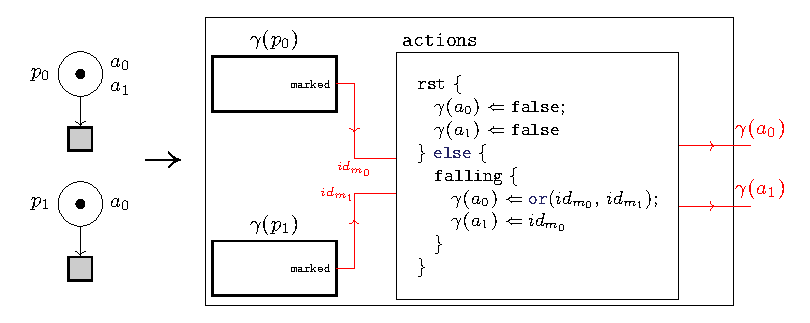
\includegraphics[keepaspectratio,width=\textwidth]{gen-actions.eps}
    \caption{The content of the \texttt{actions} process (on the
      right) based on the place-action associations of the input SITPN
      model (on the left). }
    \label{fig:gen-actions}
  \end{figure}

  \bigskip
  
  \begin{enumerate}[resume]
  \item\label{it:cond-ports} For all association between a transition and a condition, the
    input port (referred to as a \textit{condition} port) reflecting
    the Boolean value of the given condition is connected as follows
    to the input port map of the TDI corresponding to the associated
    transition:
    \begin{equation*}
      \begin{aligned}[t]
        \forall{}t&\in{}T,g_t,i_t,o_t,c\in\mathcal{C}, \\
                  & \tdiInBeh\Rightarrow \\
                  & (\mathbb{C}(t,c)=1\Rightarrow\exists{}i\in[0,\vert\mathtt{conds}(t)\vert-1]~s.t.~(\mathtt{ic}(i)\Rightarrow{}\gamma(c))\in{}i_t) \\
                  & (\mathbb{C}(t,c)=-1\Rightarrow\exists{}i\in[0,\vert\mathtt{conds}(t)\vert-1]~s.t.~(\mathtt{ic}(i)\Rightarrow{}\mathtt{not}(\gamma(c)))\in{}i_t). \\
      \end{aligned}
    \end{equation*}

  \end{enumerate}

  Figure~\ref{fig:gen-conds} illustrates the connection between a
  condition port and its associated TDIs as specified in
  Point~\ref{it:cond-ports}. Condition ports are connected to the
  \texttt{ic} (for \texttt{input\_conditions}) input port of their
  associated TDIs.
  
  \begin{figure}[h]
    \centering
    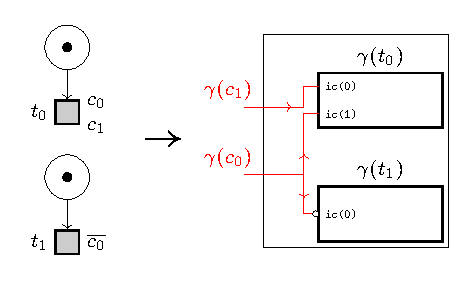
\includegraphics[keepaspectratio,width=.65\textwidth]{gen-conds.eps}
    \caption{Translation of the condition-transition associations (on
      the left) into interconnections between condition ports and
      TDIs' interfaces (on the right). }
    \label{fig:gen-conds}
  \end{figure}

  To conclude the definition of the $HM2T_{\mathtt{spec}}$ relation,
  we have $HM2T_{\mathtt{spec}}(sitpn,b,\mathtt{err})$ if $sitpn$ is
  not a well-defined SITPN model w.r.t. Definition~\ref{def:wd-sitpn}.
\end{definition}

\section{Proof of semantic preservation}
\label{sec:proof}

The semantic preservation property of the HM2T is expressed by a
\textit{forward simulation} theorem, which general form is as follows
(according to \cite{Leroy2009}):
\begin{equation*}
  \forall{}S,C,B,\mathtt{transf}(S)=C\land{}S\Downarrow{}B\Rightarrow{}\exists{}B'~s.t.~C\Downarrow{}B'\land{}B\sim{}B'.
\end{equation*}

Considering the above theorem in a more general framework than the one
of compilers from programming languages (which is the framework of
\cite{Leroy2009}), $S$ corresponds to an instance of a source
formalism, and $C$ is the result of the transformation of $S$ by the
transformation function $\mathtt{transf}$; $C$ is an instance of a
target formalism. $B$ and $B'$ are behaviors, and the binary relation
$\Downarrow$ states that a given instance of a formalism has a given
behavior. $B\sim{}B'$ states that the behavior $B$ is similar to the
behavior $B'$ considering a contextual definition of the similarity
relation. The forward simulation theorem must be read as follows: for
all instance $S$ of a source formalism transformed into $C$ by
function $\mathtt{transf}$, if $S$ has a behavior $B$, then $C$ has a
behavior $B'$ that is similar to $B$. In our case, we have proved a
slightly different theorem, which has the following form:
\begin{equation*}
  \forall{}S,C,B,B',~\mathtt{transf}(S)=C\land{}S\Downarrow{}B\land{}C\Downarrow{}B'\Rightarrow{}B\sim{}B'.
\end{equation*}
In the above form, we consider that the target $C$ has the behavior
$B'$, and we no more have to prove the existence of such a behavior.
This version of the theorem focuses on the behavior similarity. Thus,
we refer to it has a behavior (or trace) similarity theorem. In our
work perspectives, we contrive to prove the first form of the theorem,
but in this article we will present the proof of the second form.

In our specific transformation case, $S$ is a SITPN model and $C$ is a
\hvhdl{} design. The behavior of a SITPN model and a \hvhdl{} design
corresponds to the execution trace computed through a certain number
of clock cycles w.r.t. semantics rules that have been presented in
Sections~\ref{subsec:hpn-particularities} and
\ref{subsec:sim-semantics}. Thus, the property of semantic
preservation for the HM2T is about comparing the execution traces of
the input SITPN model and the output \hvhdl{} design. Specifically, we
want to show that, no matter how much clock cycles are performed, the
execution traces are always
\textit{similar}. Figure~\ref{fig:trace-comparison} illustrates the
comparison of the execution traces of a SITPN model input of the HM2T
and its corresponding output design.
\begin{figure}[!ht]
  \centering
  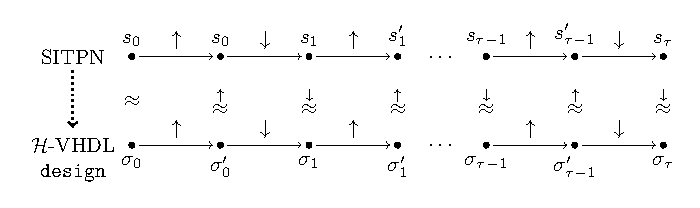
\includegraphics[keepaspectratio,width=\textwidth]{trace-comparison-full.eps}
  \caption{Comparison between the execution trace of a SITPN model (on
    the upper part) and the execution trace of the \hvhdl{} design
    resulting from the HM2T (on the lower part). The $\uparrow$
    (resp. $\downarrow$) symbol represents a rising (resp. falling)
    edge step happening in the course of a clock cycle. The $\approx$
    symbol represents the similarity relation between the upper SITPN
    state and the lower \hvhdl{} design state.}
  \label{fig:trace-comparison}
\end{figure}

In Figure~\ref{fig:trace-comparison}, $\tau$ indicates an arbitrary
number of clock cycles. To perform the proof of semantic preservation,
we must prove that every pair of states considered at the same time
point are similar w.r.t. to our own similarity relation.  Let us
introduce our general similarity criterions between a SITPN state and
a \hvhdl{} state through the relation presented in
Definition~\ref{def:state-sim}.

\begin{definition}[State similarity relation]
  \label{def:state-sim}
  For a given $sitpn\in{}SITPN$, a \hvhdl{} design $d\in{}design$, and
  a binder $\gamma\in{}WM(sitpn,d)$, an SITPN state $s\in{}S(sitpn)$
  and a design state $\sigma\in\Sigma$ are similar, written
  $\gamma\vdash{}s\approx\sigma$ if
  \begin{enumerate}
  \item\label{item:sim-mark} $\forall{}p\in{}P,$
    $~s.M(p)=\sigma(\gamma(p))($\texttt{s\_marking}$)$.
  \item\label{item:sim-tc}
    $\forall{}t\in{}T_i,$\\
    $\big(u(I_s(t))=\infty\land{}s.I(t)\le{}l(I_s(t))\Rightarrow{}s.I(t)=\sigma(\gamma(t))($\texttt{s\_time\_counter}$)\big)$\\
    $\land\big(u(I_s(t))=\infty\land{}s.I(t)>{}l(I_s(t))\Rightarrow{}\sigma(\gamma(t))($\texttt{s\_time\_counter}$)=l(I_s(t))\big)$\\
    $\land\big(u(I_s(t))\neq\infty\land{}s.I(t)>{}u(I_s(t))\Rightarrow{}\sigma(\gamma(t))($\texttt{s\_time\_counter}$)=u(I_s(t))\big)$\\
    $\land\big(u(I_s(t))\neq\infty\land{}s.I(t)\le{}u(I_s(t))\Rightarrow{}s.I(t)=\sigma(\gamma(t))($\texttt{s\_time\_counter}$)\big)$.
  \item\label{item:sim-reset} $\forall{}t\in{}T_i,$
    $s.reset_t(t)=\sigma(\gamma(t))($\texttt{s\_reinit\_time\_counter}$)$.
  \item\label{item:sim-cond}
    $\forall{}c\in\mathcal{C},~s.cond(c)=\sigma(\gamma(c))$.
  \item\label{item:sim-act}
    $\forall{}a\in\mathcal{A},~s.ex(a)=\sigma(\gamma(a))$.
  \item\label{item:sim-fun}
    $\forall{}f\in\mathcal{F},~s.ex(f)=\sigma(\gamma(f))$.
  \end{enumerate}
\end{definition}

In Definition~\ref{def:state-sim}, the binder structure $\gamma$ that
is generated by the HM2T relates the elements of the SITPN model to
the elements of the \hvhdl{} design, and thus enables the comparison
between the SITPN state and the design state. In
Definition~\ref{def:state-sim}, Point~\ref{item:sim-mark} relates the
marking value of a place $p$ at state $s$ to the value of the
\texttt{s\_marking} signal, which is an internal signal of the PDI
identified by $\gamma(p)$. Here, the expression $\sigma(\gamma(p))$
returns the internal state of the PDI $\gamma(p)$ by looking up the
component store of state $\sigma$. Point~\ref{item:sim-tc} (resp.
Point~\ref{item:sim-reset} similarly relate the value of time counters
(resp. reset orders) of transitions to the value of the
$\texttt{s\_time\_counter}$ signal
(resp. $\texttt{s\_reinit\_time\_counter}$) in the internal state of
the corresponding TDIs. In Point~\ref{item:sim-cond}
(resp. \ref{item:sim-act} and \ref{item:sim-fun}), the Boolean value
of conditions (resp. actions and functions) are compared to the value
of the input (resp. output) ports of the output design, also based on
the $\gamma$ binder.  As one can observe in Point~\ref{item:sim-tc},
due to the specific implementation of time intervals with an infinite
upper bound in \hvhdl{}, the relation between the value of a time
counter and the value of the $\texttt{s\_time\_counter}$ signal can
not be restricted to a simple equality.

As shown in Figure~\ref{fig:trace-comparison}, we make a distinction
between the state similarity after a rising edge phase and after a
falling edge phase. The definitions of the post rising edge similarity
relation, written $\stackrel{\uparrow}{\approx}$, and the post falling
edge similarity relation, written $\stackrel{\uparrow}{\approx}$, are
restrictions of the general definition. After a rising edge phase, the
equality between the value of conditions and the value of condition
ports (i.e. Point~\ref{item:sim-cond} of
Definition~\ref{def:state-sim}) does not hold, and after a falling
edge phase, the equality between the value of time counter reset
orders and the value of the \texttt{s\_reinit\_time\_counter} signals
(i.e. Point~\ref{item:sim-reset} of Definition~\ref{def:state-sim})
does not hold. However, these divergences do not impact the
computation logic of the overall so that to create further behavioral
divergences between the input SITPN model and the output \hvhdl{}
design.

Definition~\ref{def:exec-trace-sim} introduces the relation that
states that a SITPN model's execution trace is similar to a \hvhdl{}
design's execution trace.

\begin{definition}[Execution trace similarity]
  \label{def:exec-trace-sim}
  For a given $sitpn\in{}SITPN$, a \hvhdl{} design $d\in{}design$, and
  a binder $\gamma\in{}WM(sitpn,d)$, the execution trace
  $\theta_s\in{}\mathtt{list}(S(sitpn))$ and the simulation trace
  $\theta_\sigma\in\mathtt{list}(\Sigma)$ are similar, written
  $\gamma\vdash{}\theta_s\stackrel{clk}{\sim}\theta_\sigma$ where
  $clk\in\{\uparrow,\downarrow\}$, according to the following rules:\\

  \begin{tabular}{@{}l}
    {\begin{prooftree}[template={\inserttext}]        
        \infer0[$clk\in{}\{\uparrow,\downarrow\}$]{$\gamma\vdash{}[~]\stackrel{clk}{\sim}{}[~]$}
      \end{prooftree}} 
  \end{tabular}
  \begin{tabular}{@{}l}
    {\begin{prooftree}[template={\inserttext}]

        \hypo{$\gamma\vdash{}s\stackrel{\uparrow}{\sim}\sigma$}
        \hypo{$\gamma\vdash{}\theta_s\stackrel{\downarrow}{\sim}{}\theta_\sigma$}
        \infer2{$\gamma\vdash{}(s :: \theta_s)\stackrel{\uparrow}{\sim}{}(\sigma :: \theta_\sigma)$}
      \end{prooftree}} 
  \end{tabular}
  \begin{tabular}{@{}l}
    {\begin{prooftree}[template={\inserttext}]

        \hypo{$\gamma\vdash{}s\stackrel{\downarrow}{\sim}\sigma$}
        \hypo{$\gamma\vdash{}\theta_s\stackrel{\uparrow}{\sim}{}\theta_\sigma$}
        \infer2{$\gamma\vdash{}(s :: \theta_s)\stackrel{\downarrow}{\sim}{}(\sigma :: \theta_\sigma)$}
      \end{prooftree}} 
  \end{tabular}
\end{definition}

In Definition~\ref{def:exec-trace-sim}, the clock event symbol on top
of the $\sim$ sign indicates the kind of clock event that led to the
production of the states at the head of the traces. The execution
trace similarity relation expects that the states composing the traces
have been alternatively produced by a rising edge step followed by a
falling edge step. By construction, the traces must have the same
length to respect the execution trace similarity relation.

To handle the case of an execution/simulation trace beginning by an
initial state, that is, a state neither reached after a rising nor
after a falling edge, we give a slightly different definition of the
execution trace similarity relation in
Definition~\ref{def:full-exec-trace-sim}.

\begin{definition}[Full execution trace similarity]
  \label{def:full-exec-trace-sim} For a given $sitpn\in{}SITPN$, a
  \hvhdl{} design $d\in{}design$, and a binder
  $\gamma\in{}WM(sitpn,d)$, the execution trace
  $\theta_s\in{}\mathtt{list}(S(sitpn))$ and the simulation trace
  $\theta_\sigma\in\mathtt{list}(\Sigma)$ are fully similar, written
  $\gamma\vdash{}\theta_s\sim\theta_\sigma$, according to the
  following rules:\\

  \begin{tabular}{l}
    {\begin{prooftree}[template={\inserttext}]
        \infer0{$\gamma\vdash{}[~]\sim{}[~]$}
      \end{prooftree}}
  \end{tabular}
  \begin{tabular}{l}
    {\begin{prooftree}[template={\inserttext}]

        \hypo{$\gamma\vdash{}s\sim\sigma$}
        \hypo{$\gamma\vdash{}\theta_s\stackrel{\uparrow}{\sim}{}\theta_\sigma$}
        \infer2{$\gamma\vdash{}(s :: \theta_s)\sim{}(\sigma ::
          \theta_\sigma)$}
      \end{prooftree}}
  \end{tabular}
\end{definition}

The full execution trace similarity relation indicates that the head
states of traces must verify the general state similarity relation
(cf. Figure~\ref{fig:trace-comparison}), and that the tail of the
traces must respect the execution state similarity relation starting
with a rising edge step.

Now, let us introduce the necessary lemmas to prove the semantic
preservation theorem. In Definition~\ref{def:hm2t-hyps}, we present
the hypotheses expressing the fact that we are proving the semantic
preservation property for the HM2T. These hypotheses will always
appear in the lemmas and theorems presented afterwards.

\begin{definition}[HM2T hypotheses]
  \label{def:hm2t-hyps}
  For all well-defined $sitpn\in{}SITPN$, bounding function
  $b\in{}P\rightarrow\mathbb{N}$, \hvhdl{} design $d\in{}design$,
  binder $\gamma\in{}WM(sitpn,d)$, elaborated design
  $\Delta\in{}ElDesign$, default state $\sigma_e\in\Sigma$, simulation
  environment $E_p\in\mathbb{N}\rightarrow{}(id\nrightarrow{}v)$, and
  execution environment
  $E_c\in\mathbb{N}\rightarrow(\mathcal{C}\rightarrow\mathbb{B})$,
  assume that:
  \begin{enumerate}
  \item\label{it:HM2T-some} Taking the SITPN model $sitpn$ and the
    bounding function $b$ as inputs, the HM2T returns an output design
    $d$ and a binder $\gamma$, written
    $\mathtt{sitpn2hvhdl}(sitpn, b)=\lfloor(d,\gamma)\rfloor$ where
    $\mathtt{sitpn2hvhdl}\in{}SITPN\rightarrow(P\rightarrow\mathbb{N})\nrightarrow(design\times{}WM(sitpn,d))$.
  \item\label{it:sitpn-is-bounded} $sitpn$ is bounded through $b$,
    written $\lceil{}sitpn\rceil^b$.
  \item In the context of the \hilecop{} design store
    $\mathcal{D}_\mathcal{H}$ and with an empty generic constant
    dimensioning function ($\emptyset$), $d$ is elaborated into
    $\Delta$ with a default state $\sigma_e$, written
    $\mathcal{D}_\mathcal{H},\emptyset\vdash{}d\xrightarrow{elab}\Delta,\sigma_e$.
  \item\label{it:env-are-sim} Simulation and execution environments
    are similar, written $\gamma\vdash{}E_p\stackrel{env}{=}E_c$.
  \end{enumerate}
  
\end{definition}

In Point~\ref{it:HM2T-some} of Definition~\ref{def:hm2t-hyps}, the
$\mathtt{sitpn2hvhdl}$ function implements the HM2T, that is a
function proved sound and complete w.r.t. to the specification
presented in Section~\ref{sec:m2t}. Point~\ref{it:sitpn-is-bounded}
expresses the boundedness property of the input SITPN
model. Point~\ref{it:env-are-sim} states that, at each time point, the
execution and simulation environments yield the same Boolean value for
all couple condition-condition port linked through $\gamma$.

\def\hm2thyps{well-defined $sitpn\in{}SITPN$,
  $b\in{}P\rightarrow\mathbb{N}$, $d\in{}design$,
  $\gamma\in{}WM(sitpn,d)$, $\Delta\in{}ElDesign,\sigma_{e}\in\Sigma$,
  $E_p\in\mathbb{N}\rightarrow{}(id\nrightarrow{}v)$, and
  $E_c\in\mathbb{N}\rightarrow(\mathcal{C}\rightarrow\mathbb{B})$ that
  verify the hypotheses of Definition~\ref{def:hm2t-hyps}}

As illustrated in Figure~\ref{fig:trace-comparison}, to prove that the
execution traces are similar, we must first prove that the two initial
states are similar. This is expressed by
Lemma~\ref{lem:sim-init-states}.
\begin{lemma}[Similar initial states]
  \label{lem:sim-init-states}
  For all \hm2thyps{}, and for all $\sigma_0,\sigma_i\in{}\Sigma$ such that:
  \begin{itemize}
  \item $\sigma_0$ is the initial state of design $d$:\\
    $\mathcal{D},\Delta,\sigma_e\vdash{}d.beh\xrightarrow{cs_i}{}\sigma_i$ and
    $\mathcal{D},\Delta,\sigma_i\vdash{}d.beh\xrightarrow{\rightsquigarrow}{}\sigma_0$
  \end{itemize}
  then $\gamma\vdash{}s_0\approx\sigma_0$.
\end{lemma}

Starting from two similar initial states, then we must prove that each
phase, or step, of a clock cycle produces still similar states.  This
is expressed by \textit{lock-step simulation} lemmas \cite{Leroy2009},
which are of the following form in their \textit{non-existantial}
version:
\begin{equation*}
  \forall{}S_1,S'_1,S_2,S'_2,~S1\rightarrow{}S'_1\land{}S_2\rightarrow{}S'_2\land{}S_1\approx{}S_2\Rightarrow{}S'_1\approx{}S'_2.
\end{equation*}
Here, $S_1$ and $S'_1$ are two states of the source formalism, $S_2$
and $S'_2$ are two states of the target formalism.
$S_1\rightarrow{}S'_1$ (resp. $S_2\rightarrow{}S'_2$) states that an
execution step leads from $S_1$ to $S'_1$ (resp. from $S_2$ to $S'_2$)
w.r.t. a contextual definition of the execution
step. $S_1\approx{}S_2$ indicates that $S_1$ and $S_2$ are similar,
also w.r.t. a contextual definition of state similarity. The above
theorem must be read as follows: given two similar states $S_1$ and
$S_2$, if one execution step leads from $S_1$ to $S'_1$ and from $S_2$
to $S'_2$, then $S'_1$ and $S'_2$ are similar. \\

To establish the semantic preservation property, the first lock-step
simulation lemma that we had to prove pertains to the first rising
edge step. As defined in the SITPN semantics, the first rising edge
step is idle, i.e. a SITPN model is still in its initial state after
this step. Thus, we must prove that the state of the output design
reached after the first rising edge is similar to the SITPN model's
initial state. This is expressed by Lemma~\ref{lem:fst-re-lock-step}.

\begin{lemma}[First rising edge lock-step simulation]
  \label{lem:fst-re-lock-step}
  For all \hm2thyps{}, and for all clock count $\tau\in\mathbb{N}$,
  $\sigma_0,\sigma_i,\sigma_{\uparrow},\sigma'_0\in{}\Sigma$ such that:
  \begin{itemize}
  \item $\sigma_0$ is the initial state of design $d$:\\
    $\mathcal{D},\Delta,\sigma_e\vdash{}d.beh\xrightarrow{cs_i}{}\sigma_i$ and
    $\mathcal{D},\Delta,\sigma_i\vdash{}d.beh\xrightarrow{\rightsquigarrow}{}\sigma_0$
    
  \item a rising edge step leads from $\sigma_0$ to $\sigma'_0$:\\
    $\mathcal{D}_\mathcal{H},\Delta,\mathtt{inj}(\sigma_0,E_p,\tau)\vdash{}d.beh\xrightarrow{cs_{\uparrow}}\sigma_{\uparrow}$
    and
    $\mathcal{D}_\mathcal{H},\Delta,\sigma_{\uparrow}\vdash{}d.beh\xrightarrow{\rightsquigarrow}\sigma'_0$
  \end{itemize}
  then $\gamma\vdash{}s_0\stackrel{\uparrow}{\approx}\sigma'_0$.
\end{lemma}
In Lemma~\ref{lem:fst-re-lock-step}, $s_0$ is the initial state of the
SITPN model as introduced in
Definition~\ref{def:sitpn-init-state}.  Note that a rising edge step on the \hvhdl{} side refers to the conjunction of the three following phases: the injection of fresh values in primary input ports (through the use of the \texttt{inj} function), the execution of rising blocks, and the stabilization of combinational parts. \\

Then, we must prove that any rising edge or falling edge step verifies
the lock-step simulation property. This is expressed by
Lemmas~\ref{lem:re-lock-step} and \ref{lem:fe-lock-step}. 

\begin{lemma}[Rising edge lock-step simulation]
  \label{lem:re-lock-step}
  For all \hm2thyps{}, and for all $\tau\in\mathbb{N}$,
  $s,s'\in{}S(sitpn)$, $\sigma,\sigma_\uparrow,\sigma'\in\Sigma$, such
  that
  \begin{itemize}
  \item $s$ and $\sigma$ are similar states as intended after a
    falling edge step:
    $\gamma\vdash{}s\stackrel{\downarrow}{\approx}\sigma$
  \item a rising edge step leads from $s$ to $s'$:
    $E_c,\tau\vdash{}s\xrightarrow{\uparrow}s'$
  \item a rising edge step leads from $\sigma$ to $\sigma'$:\\
    $\mathcal{D}_\mathcal{H},\Delta,\mathtt{inj}(\sigma,E_p,\tau)\vdash{}d.beh\xrightarrow{cs_{\uparrow}}\sigma_{\uparrow}$
    and
    $\mathcal{D}_\mathcal{H},\Delta,\sigma_{\uparrow}\vdash{}d.beh\xrightarrow{\rightsquigarrow}\sigma'$
  \end{itemize}
  then $\gamma\vdash{}s'\stackrel{\uparrow}{\approx}{}\sigma'$.
  
\end{lemma}

\begin{lemma}[Falling edge lock-step simulation]
  \label{lem:fe-lock-step}
  For all \hm2thyps{}, and for all $\tau\in\mathbb{N}$,
  $s,s'\in{}S(sitpn)$, $\sigma,\sigma_\downarrow,\sigma'\in\Sigma$,
  such that
  \begin{itemize}
  \item $s$ and $\sigma$ are similar states as intended after a rising
    edge step: $\gamma\vdash{}s\stackrel{\downarrow}{\approx}\sigma$
  \item a falling edge step leads from $s$ to $s'$:
    $E_c,\tau\vdash{}s\xrightarrow{\downarrow}s'$
  \item a falling edge step leads from $\sigma$ to $\sigma'$:\\
    $\mathcal{D}_\mathcal{H},\Delta,\sigma\vdash{}d.beh\xrightarrow{cs_{\downarrow}}\sigma_{\downarrow}$
    and
    $\mathcal{D}_\mathcal{H},\Delta,\sigma_{\downarrow}\vdash{}d.beh\xrightarrow{\rightsquigarrow}\sigma'$
  \end{itemize}
  then $\gamma\vdash{}s'\stackrel{\downarrow}{\approx}{}\sigma'$.
\end{lemma}

As expressed in Lemma~\ref{lem:fe-lock-step}, a falling edge step on
the \hvhdl{} side refers to the execution of falling blocks followed
by the stabilization of combinational parts.\\

Under the assumptions of Lemma~\ref{lem:sim-init-states},
\ref{lem:fst-re-lock-step}, \ref{lem:re-lock-step} and
\ref{lem:fe-lock-step}, we can now prove the following trace
similarity theorem expressing that the HM2T is semantic preserving.

\begin{theorem}[Full trace similarity]
  \label{thm:full-trace-sim}
  For all well-defined $sitpn\in{}SITPN$, bounding function
  $b\in{}P\rightarrow\mathbb{N}$, \hvhdl{} design $d\in{}design$,
  binder $\gamma\in{}WM(sitpn,d)$, default state $\sigma_e\in\Sigma$,
  simulation environment
  $E_p\in\mathbb{N}\rightarrow{}(id\nrightarrow{}v)$, execution
  environment
  $E_c\in\mathbb{N}\rightarrow(\mathcal{C}\rightarrow\mathbb{B})$,
  $\tau\in\mathbb{N}$, SITPN model trace
  $\theta_s\in\mathtt{list}(S(sitpn))$, and \hvhdl{} design trace
  $\theta_\sigma\in\mathtt{list}(\Sigma)$ such that:
  \begin{enumerate}
  \item $\mathtt{sitpn2hvhdl}(sitpn, b)=\lfloor(d,\gamma)\rfloor$
  \item $\lceil{}sitpn\rceil^b$
  \item $\gamma\vdash{}E_p\stackrel{env}{=}E_c$
  \item $E_c,\tau\vdash{}sitpn\xrightarrow{full}\theta_s$
  \item
    $\mathcal{D}_\mathcal{H},\emptyset,E_p,\tau\vdash{}d\xrightarrow{full}\theta_\sigma$
  \end{enumerate}
  then $\gamma\vdash\theta_s\sim\theta_\sigma$.
\end{theorem}

\begin{pf}[Proof of Theorem~\ref{thm:full-trace-sim}.]
  
  Proceeding by case analysis on the number of clock cycles $\tau$,
  there are two cases. First $\tau=0$, and then we must prove that the
  initial states are similar, which is true appealing to
  Lemma~\ref{lem:sim-init-states}. Otherwise, $\tau>0$ and then at
  least the first clock cycle is executed. Thanks to
  Lemmas~\ref{lem:fst-re-lock-step} and \ref{lem:fe-lock-step}, we can
  show that the states are similar during the first clock cycle. Then,
  we can reason by induction over $\tau$ to prove that the remnant of
  the execution traces are similar. We can appeal to
  Lemmas~\ref{lem:re-lock-step} and \ref{lem:fe-lock-step} to prove
  that states are similar during the induction step (corresponding to
  an arbitrary clock cycle step), and then use the induction
  hypothesis to complete the proof.

\end{pf}

\subsection{A mechanization-ready proof}
\label{sec:mecha-ready-pf}

As presented above, proving Theorem~\ref{thm:full-trace-sim} amounts
to proving Lemma~\ref{lem:sim-init-states}, which is about the
similarity of the initial states, and the different lock-step
simulation lemmas (i.e. Lemmas~\ref{lem:fst-re-lock-step},
\ref{lem:re-lock-step} and \ref{lem:fe-lock-step}). Preparing for the
mechanization of the proof of Theorem~\ref{thm:full-trace-sim} with
the \coq{} proof assistant, we have written a very detailed proof (a
hundred-page long) for Lemmas~\ref{lem:sim-init-states},
\ref{lem:fst-re-lock-step}, \ref{lem:re-lock-step} and
\ref{lem:fe-lock-step}. The full proof is available in
\cite{Iampietro2021}. Even though obviously a tedious task, writing
the fully detailed proof before the mechanization has been a
successful process. It has revealed a bug in the \vhdl{} code defining
the behavior of the place design. This bug has been corrected in the
version of the place design given in Appendix~\ref{app:place-design}.
Due to the important amount of work demanded by the mechanization
task, if we had tackled down the mechanization of the proof without a
previously
detailed proof plan, this bug would not have yet been detected. \\

To illustrate the level of details of our proof, let us present an
extract of the proof of
Lemma~\ref{lem:re-lock-step}. Lemma~\ref{lem:re-lock-step} states that
the rising edge step verifies the lock-step simulation property. To
prove that the states of the input SITPN model and the output design
are similar after a rising edge step, we must prove, among other
points, that the marking of a given place is equal to the value the
\texttt{s\_marking} internal signal in its corresponding PDI. This is
expressed by Lemma~\ref{lem:re-eq-marking}.

\begin{lemma}[Rising edge equal marking]
  \label{lem:re-eq-marking}
  For all \hm2thyps{}, and for all $\tau\in\mathbb{N}$,
  $s,s'\in{}S(sitpn)$, $\sigma,\sigma_\uparrow,\sigma'\in\Sigma$, such
  that
  \begin{itemize}
  \item $s$ and $\sigma$ are similar states as intended after a
    falling edge step:
    $\gamma\vdash{}s\stackrel{\downarrow}{\approx}\sigma$
  \item a rising edge step leads from $s$ to $s'$:
    $E_c,\tau\vdash{}s\xrightarrow{\uparrow}s'$
  \item a rising edge step leads from $\sigma$ to $\sigma'$:\\
    $\mathcal{D}_\mathcal{H},\Delta,\mathtt{inj}(\sigma,E_p,\tau)\vdash{}d.beh\xrightarrow{cs_{\uparrow}}\sigma_{\uparrow}$
    and
    $\mathcal{D}_\mathcal{H},\Delta,\sigma_{\uparrow}\vdash{}d.beh\xrightarrow{\rightsquigarrow}\sigma'$
  \end{itemize}
  then
  $\forall{}p\in{}P,~s'.M(p)=\sigma'(\gamma(p))(\mathtt{s\_marking})$.
  
\end{lemma}

\begin{pf}[Proof of Lemma~\ref{lem:re-eq-marking}.]
  Given all the elements and assuming all the hypotheses expressed in
  Lemma~\ref{lem:re-eq-marking}, then, given a place $p\in{}P$, let us
  show that:
  \begin{equation*}
    \boxed{s'.M(p)=\sigma'(\gamma(p))(\texttt{s\_marking})}
  \end{equation*}

  By definition of the SITPN state transition relation on rising edge
  (cf. Definition~\ref{def:semantics}, Point~\ref{it:new-marking}), we
  have:
  \begin{equation}\label{eq:re-eq-marking-eqmp}
    s'.M(p)=s.M(p)-\sum\limits_{t\in{}Fired(s)}pre(p,t)+\sum\limits_{t\in{}Fired(s)}post(t,p)
  \end{equation}

  \bigskip
  
  By definition of the HM2T (cf. Definition~\ref{def:hm2t-spec},
  Point~\ref{it:pdi-exists}), there exists $g_p,i_p,o_p$ such that
  $\mathtt{comp}(\gamma(p),\mathtt{place},g_p,i_p,o_p)\in{}d.beh$.  By
  property of the \hvhdl{} concurrent statement execution relation
  (cf. Table~\ref{tab:cs-eval}), the stabilization relation
  (cf. Table~\ref{tab:stabilization}),
  $\mathtt{comp}(\gamma(p),\mathtt{place},g_p,i_p,o_p)\in{}d.beh$, and
  through the examination of the \texttt{marking} process defined in
  the behavior of the place design (Appendix~\ref{app:place-design},
  Line~49), we can deduce that the following equation holds:
  \begin{equation}\label{eq:re-eq-marking-eqsm}
    \begin{split}
      \sigma'(\gamma(p))(\texttt{sm})=\sigma(\gamma(p))(\texttt{sm})-\sigma(\gamma(p))(\texttt{s\_output\_token\_sum})\\
      +\sigma(\gamma(p))(\texttt{s\_input\_token\_sum})
    \end{split}
  \end{equation}

  \bigskip
  
  \noindent{}Rewriting the goal with \eqref{eq:re-eq-marking-eqmp} and
  \eqref{eq:re-eq-marking-eqsm}, we must show that:
  \begin{equation*}
    \boxed{
      \begin{array}{c}
      s.M(p)-\sum\limits_{t\in{}Fired(s)}pre(p,t)+\sum\limits_{t\in{}Fired(s)}post(t,p)\\
      = \\
      \sigma(\gamma(p))(\texttt{sm})-\sigma(\gamma(p))(\texttt{sots})
      +\sigma(\gamma(p))(\texttt{sits}) \\
      \end{array}}
  \end{equation*}
  
  \bigskip
  
  By definition of the state similarity relation
  (cf. Definition~\ref{def:state-sim}, Point~\ref{item:sim-mark}), we
  can deduce that $s.M(p)=\sigma(\gamma(p))(\texttt{sm})$. Then, two
  points remain to be shown to complete the proof:
  \begin{enumerate}
  \item $\sum\limits_{t\in{}Fired(s)}pre(p,t)=\sigma(\gamma(p))(\texttt{sots})$
  \item $\sum\limits_{t\in{}Fired(s)}post(t,p)=\sigma(\gamma(p))(\texttt{sits})$
  \end{enumerate}

  \bigskip
  
  We will only detail the proof of the second point. The \texttt{sits}
  signal is an internal signal of the place design. It is a
  \textit{combinational} signal, that is, an equation relates its
  value to the value of other signals, and this equation holds at any
  moment in the execution of the design.  In the case of the
  \texttt{sits} signal, the \texttt{input\_tokens\_sum} process
  defines the related combinational equation.  Thus, by property of
  the stabilization relation (cf. Table~\ref{tab:stabilization}),
  $\mathtt{comp}(\gamma(p),\mathtt{place},g_p,i_p,o_p)\in{}d.beh$, and
  through the examination of the \texttt{input\_tokens\_sum} process
  defined in the behavior of the place design
  (Appendix~\ref{app:place-design}, Line~29), we can deduce that the
  following equation holds:
  \begin{equation}
    \label{eq:sits-at-fe}
    \sigma(\gamma(p))(\texttt{sits})=\sum\limits_{i=0}^{\Delta(\gamma(p))(\texttt{ian})-1}
    \begin{cases}
      \sigma(\gamma(p))(\texttt{iaw})[i]~\mathtt{if}~\sigma(\gamma(p))(\texttt{itf})[i]\\
      0~otherwise \\
    \end{cases}
  \end{equation}

  \noindent{}Rewriting the goal with \eqref{eq:sits-at-fe}:\\
  \begin{equation*}
    \boxed{
      \sum\limits_{t\in{}Fired(s)}post(t,p)=\sum\limits_{i=0}^{\Delta(\gamma(p))(\texttt{ian})-1}
      \begin{cases}
        \sigma(\gamma(p))(\texttt{iaw})[i]~\mathtt{if}~\sigma(\gamma(p))(\texttt{otf})[i]\\
        0~otherwise \\
      \end{cases}}
  \end{equation*}

  \bigskip
  
  \noindent{}Let us unfold the definition of the left sum term:\\
  \begin{equation*}
    \boxed{\begin{array}{c}
      \sum\limits_{t\in{}Fired(s)}
      \begin{cases}
        \omega~\mathtt{if}~post(t,p)=\lfloor\omega\rfloor \\
        0~otherwise
      \end{cases} \\
      = \\
      \sum\limits_{i=0}^{\Delta(\gamma(p))(\texttt{ian})-1}
      \begin{cases}
        \sigma(\gamma(p))(\texttt{iaw})[i]~\mathtt{if}~\sigma(\gamma(p))(\texttt{itf})[i]\\
        0~otherwise \\
      \end{cases} \\
    \end{array}}
  \end{equation*}

  \bigskip
  
  \noindent{}Let us perform case analysis on $\mathtt{input}(p)$;
  there are two cases:

  \begin{itemize}
  \item \textbf{CASE} $\mathtt{input}(p)=\emptyset$:\\
    
    By definition of the HM2T (cf. \cite{Iampietro2022hfspec} to see
    the case where $\mathtt{input}(p)=\emptyset$), we have
    $(\mathtt{ian}\Rightarrow{}1)\in{}g_p$,
    $(\mathtt{itf}(0)\Rightarrow{}\mathtt{true})\in{}i_p$, and
    $(\mathtt{iaw}(0)\Rightarrow{}0)\in{}i_p$.

    By property of the elaboration relation, and knowing that
    $\mathtt{comp}(\gamma(p),\mathtt{place},g_p,i_p,o_p)\in{}d.beh$,
    $(\mathtt{ian}\Rightarrow{}1)\in{}g_p$,
    $(\mathtt{itf}(0)\Rightarrow{}\mathtt{true})\in{}i_p$, and
    $(\mathtt{iaw}(0)\Rightarrow{}0)\in{}i_p$, we can deduce that the
    following equations hold:
    \begin{eqnarray}
      \label{eq:eq-ian-itfz-iawz-0}
      \Delta(\gamma(p))(\texttt{ian})&=&1 \\
      \label{eq:eq-ian-itfz-iawz-1}\sigma(\gamma(p))(\texttt{itf})[0]&=&\mathtt{true} \\
      \label{eq:eq-ian-itfz-iawz-2}\sigma(\gamma(p))(\texttt{iaw})[0]&=&0
    \end{eqnarray}

    By property of $\mathtt{input}(p)=\emptyset$, we can deduce:
    \begin{equation}
      \sum\limits_{t\in{}Fired(s)}
      \begin{cases}
        \omega~\mathtt{if}~post(t,p)=\lfloor\omega\rfloor \\
        0~otherwise
      \end{cases}=0.
      \label{eq:post-sum-eq-z}    
    \end{equation}

    \noindent{}Rewriting the goal with \eqref{eq:eq-ian-itfz-iawz-0},
    \eqref{eq:eq-ian-itfz-iawz-1}, \eqref{eq:eq-ian-itfz-iawz-2} and
    \eqref{eq:post-sum-eq-z}, we arrive to a tautology.\\
    
  \item \textbf{CASE} $input(p)\neq\emptyset$:\\

    By definition of the HM2T (Definition~\ref{def:hm2t-spec},
    Point~\ref{it:pdi-gmap}), we have
    $(\mathtt{ian}\Rightarrow{}\vert{}input(p)\vert)\in{}g_p$, and by
    property of the elaboration relation, we can deduce:
    \begin{equation}
      \Delta(\gamma(p))(\texttt{ian})=\vert{}input(p)\vert\label{eq:ian-eq-input-card}
    \end{equation}

    To ease the reading, let us define functions
    $f\in{}Fired(s)\rightarrow\mathbb{N}$ and
    $g\in[0,\vert{}input(p)\vert-1]\rightarrow\mathbb{N}$ s.t. $f(t)=
    \begin{cases}
      \omega~\mathtt{if}~post(t,p)=\lfloor\omega\rfloor \\
      0~otherwise
    \end{cases}$
    and $g(i)=
    \begin{cases}
      \sigma(\gamma(p))(\texttt{iaw})[i]~\mathtt{if}~\sigma(\gamma(p))(\texttt{itf})[i]\\
      0~otherwise 
    \end{cases}$.

    \noindent{}The goal can be expressed as follows:
    \begin{equation*}
      \boxed{\sum\limits_{t\in{}Fired(s)}f(t)=\sum\limits_{i=0}^{\Delta(\gamma(p))(\texttt{ian})-1}g(i)}
    \end{equation*}
    
    \noindent{}Rewriting the goal with \eqref{eq:ian-eq-input-card}, we must show:
    \begin{equation*}
      \boxed{\sum\limits_{t\in{}Fired(s)}f(t)=\sum\limits_{i=0}^{\vert{}input(p)\vert-1}g(i)}
    \end{equation*}

    Now, we must prove the above equality between two sums. We had to
    prove a lot of such equalities during the entire proof. Thus, we
    came up with Theorem~\ref{thm:sums-equal} that presents a set of
    sufficient conditions to prove that two sums are equal.
    \todo[inline]{Mettre la preuve du theoreme en annexe?}
    
    \begin{theorem}[Equality between two sums]
      \label{thm:sums-equal}
      For all sets $X,Y,A,B$ such that $A\subseteq{}X$ and
      $Y\subseteq{}X$, and for all functions
      $f\in{}A\rightarrow\mathbb{N}$, $g\in{}B\rightarrow\mathbb{N}$,
      if there exists $\beta\in{}Y\rightarrow{}B$ such that:
      \begin{itemize}
      \item $\beta$ is a bijection
      \item $\forall{}a\in{}A\cap{}Y,~f(a)=g(\beta(a))$
      \item $\forall{}a\in{}A\setminus{}Y,~f(a)=0$
      \item $\forall{}b\in{}B,\beta^{-1}(b)\notin{}A\Rightarrow{}g(b)=0$
      \end{itemize}
      then $\sum\limits_{a\in{}A}f(a)=\sum\limits_{b\in{}B}g(b)$.
    \end{theorem}
    
    By property of the HM2T, there exists a bijection
    $\beta\in\mathtt{input}(p)\rightarrow{}[0,\vert{}input(p)\vert-1]$
    such that:
    \begin{equation}
      \label{eq:bij-input}
      \begin{aligned}[t]
        \forall{}t&\in{}T,g_t,i_t,o_t,g_p,i_p,o_p,\omega\in\mathbb{N}^{*}, \\
                  & post(t,p)=\lfloor\omega\rfloor\Rightarrow \\
                  & \tdiInBeh\Rightarrow \\
                  & \pdiInBeh\Rightarrow\\
                  &
                    \begin{aligned}[t]
                      & (\mathtt{iaw}(\beta(t))\Rightarrow\omega)\in{}i_p \\
                      & \begin{aligned}[t]
                          \land\exists{}id_s~&s.t.~(id_s,\mathtt{bool})\in{}d.sigs \\
                                             & \land(\mathtt{fired}\Rightarrow{}id_s)\in{}o_t\land(\mathtt{itf}(\beta(t))\Rightarrow{}id_s)\in{}i_p.\\
                        \end{aligned} \\
                    \end{aligned}
        \\
      \end{aligned}
    \end{equation}

    Let us take $\beta$ and appeal to Theorem~\ref{thm:sums-equal} to
    prove the goal. Then, it suffices to show that:
    \begin{enumerate}
    \item $\beta$ is a bijection
    \item $\forall{}t\in{}Fired(s)\setminus{}\mathtt{input}(p),~f(t)=0$
    \item $\forall{}t\in{}Fired(s)\cap{}\mathtt{input}(p),~f(t)=g(\beta(t))$
    \item
      $\forall{}i\in{}[0,\vert\mathtt{input}(p)\vert-1],\beta^{-1}(i)\notin{}Fired(s)\Rightarrow{}g(i)=0$
    \end{enumerate}

    \bigskip
    
    \begin{enumerate}
    \item By assumption, $\beta$ is a bijection.
    \item Given a $t\in{}Fired(s)\setminus{}\mathtt{input}(p)$, let us
      show $f(t)=0$, that is:
      \begin{equation*}
        \boxed{
          \begin{cases}
            \omega~\mathtt{if}~post(t,p)=\lfloor\omega\rfloor \\
            0~otherwise
          \end{cases}=0
        }
      \end{equation*}

      \noindent{}As $t\notin{}\mathtt{input}(p)$, then
      $post(t,p)=\emptyset$, and that settles the goal.
      
    \item Given a $t\in{}Fired(s)\cap\mathtt{input}(p)$, let us show
      $f(t)=g(\beta(t))$, that is:
      \begin{equation*}
        \boxed{\begin{array}{c}
          \begin{cases}
            \omega~\mathtt{if}~post(t,p)=\lfloor\omega\rfloor \\
            0~otherwise
          \end{cases} \\
          = \\
          \begin{cases}
            \sigma(\gamma(p))(\texttt{iaw})[\beta(t)]~\mathtt{if}~\sigma(\gamma(p))(\texttt{itf})[\beta(t)] \\
            0~otherwise \\
          \end{cases} \\         
        \end{array}}
      \end{equation*}


      \noindent{}By definition of $t\in{}\mathtt{input}(p)$, there
      exists a weight $\omega\in\mathbb{N}^{*}$ such that
      $post(t,p)=\lfloor\omega\rfloor$.  Thus, the goal can be
      rewritten as follows:     
      \begin{equation*}
        \boxed{\omega=
          \begin{cases}
            \sigma(\gamma(p))(\texttt{iaw})[\beta(t)]~\mathtt{if}~\sigma(\gamma(p))(\texttt{itf})[\beta(t)]~ \\
            0~otherwise \\
          \end{cases}}
      \end{equation*}

     By definition of the HM2T (Definition~\ref{def:hm2t-spec},
     Point~\ref{it:exists-tdi}), there exist $g_t,i_t,o_t$ such that
     $\mathtt{comp}(\gamma(t),\mathtt{transition}, g_t, i_t,
     o_t)\in{}d.beh$. 
     
     Then, from \eqref{eq:bij-input}, we can deduce
     $(\mathtt{iaw}(\beta(t))\Rightarrow{}\omega)\in{}i_p$, and by
     property of the stabilization relation, we can deduce
     $\sigma(\gamma(p))(\texttt{iaw})[\beta(t)]=\omega$. Thus, the goal
     can be rewritten as follows:
     \begin{equation*}
       \boxed{\omega=
       \begin{cases}
         \omega~\mathtt{if}~\sigma(\gamma(p))(\texttt{itf})[\beta(t)]~ \\
         0~otherwise \\
       \end{cases}}
     \end{equation*}
     
     From \eqref{eq:bij-input}, we can deduce that there exists an
     $id_s$ such that:
     \begin{itemize}
     \item $(id_s,\mathtt{bool})\in{}d.sigs$
     \item $(\mathtt{fired}\Rightarrow{}id_s)\in{}o_t$
     \item $(\mathtt{itf}(\beta(t))\Rightarrow{}id_s)\in{}i_p$
     \end{itemize}
     
     Let us take such an $id_s$. By property of the stabilization
     relation, and knowing that
     $(\mathtt{fired}\Rightarrow{}id_s)\in{}o_t$ and
     $(\mathtt{itf}(\beta(t))\Rightarrow{}id_s)\in{}i_p$, we can deduce
     $\sigma(\gamma(p))(\texttt{itf})[\beta(t)]=\sigma(id_s)=\sigma(\gamma(t))(\texttt{fired})$.

     \noindent{}Thus, the goal can be rewritten as follows:
     \begin{equation*}
       \boxed{       \omega=
         \begin{cases}
           \omega~\mathtt{if}~\sigma(\gamma(t))(\texttt{fired}) \\
           0~otherwise \\
         \end{cases}
       }
     \end{equation*}
   
     Now, to conclude the proof, let us assume that
     $\sigma(\gamma(t))(\texttt{fired})=\mathtt{true}$ iff
     $t\in{}Fired(s)$. This assumption comes from Lemma ``Falling edge
     equal fired'', which proof is detailed and illustrated in
     \cite[p.220]{Iampietro2021}. This lemma states that, at the end
     of a falling edge step, there is an equivalence between the set
     of fired transitions and the value of the \texttt{fired} output
     port of each corresponding TDI. Then, knowing that
     $t\in{}Fired(s)$ and that state $s$ results from the execution of
     a previous falling edge step, we can deduce
     $\sigma(\gamma(t))(\texttt{fired})=\mathtt{true}$ and then
     conclude the goal.
     
   \item Given an $i\in[0,\vert\mathtt{input}(p)\vert-1]$, and
     assuming that $\beta^{-1}(i)\notin{}Fired(s)$, let us show
     $g(i)=0$, that is:
     \begin{equation*}
       \boxed{
         \begin{cases}
           \sigma(\gamma(p))(\texttt{iaw})[i]~\mathtt{if}~\sigma(\gamma(p))(\texttt{itf})[i] \\
           0~otherwise \\
         \end{cases}=0
       }
     \end{equation*}

     Let us define $t_i=\beta^{-1}(i)$. To conclude the goal, it is sufficient to show that:
     \begin{equation*}
       \boxed{\sigma(\gamma(p))(\mathtt{itf})[i]=\mathtt{false}}
     \end{equation*}

     By definition of the HM2T, there exist
     $g_{t_i}, i_{t_i}, o_{t_i}$ such that
     $\mathtt{comp}(\gamma(t_i), \mathtt{transition}, g_{t_i},
     i_{t_i}, o_{t_i})\in{}d.beh$.

     From $t_i\in\mathtt{input}(p)$, we can deduce that there exists
     $\omega''\in\mathbb{N}^{*}$ such that
     $post(t_i, p)=\lfloor\omega''\rfloor$.

     From \eqref{eq:bij-input}, we can deduce that there exists an
     $id_{s_i}$ such that:
     \begin{itemize}
     \item $(id_{s_i},\mathtt{bool})\in{}d.sigs$
     \item $(\mathtt{fired}\Rightarrow{}id_{s_i})\in{}o_{t_i}$
     \item $(\mathtt{itf}(i)\Rightarrow{}id_{s_i})\in{}i_p$
     \end{itemize}

     Let us take such an $id_{s_i}$. By property of the stabilization
     relation, and knowing that
     $(\mathtt{fired}\Rightarrow{}id_{s_i})\in{}o_{t_i}$ and
     $(\mathtt{itf}(i)\Rightarrow{}id_{s_i})\in{}i_p$, we can deduce
     $\sigma(\gamma(p))(\texttt{itf})[i]=\sigma(id_{s_i})=\sigma(\gamma(t_i))(\texttt{fired})$.
     Thus, the goal can be rewritten as follows:
     \begin{equation*}
       \boxed{\sigma(\gamma(t_i))(\mathtt{fired})=\mathtt{false}}
     \end{equation*}

     From Lemma ``Falling edge not equal fired''
     \cite[p.351]{Iampietro2021} and knowing that
     $t_i\notin{}Fired(s)$, we can conclude the proof. Lemma ``Falling
     edge not equal fired'' states that, at the end of a falling edge
     step, for all transition that is not fired, then the value of the
     \texttt{fired} output port of the corresponding TDI is
     \texttt{false}.
   \end{enumerate}
 \end{itemize}
 
\end{pf}


\subsection{Mechanization with the \coq{} proof assistant}
\label{sec:mech-of-the-proof}

  % In this section, we give
% metrics to measure this gap. We point out some of the reasons that may
% explain the gap, and comment on some employed techniques to reduce the
% size of proof scripts. As a remainder, the full code including
% specifications and proof scripts is available at
% \url{https://github.com/viampietro/ver-hilecop}.

Listing~\ref{lst:coq-full-trace-sim-thm} presents the \coq{}
implementation of Theorem~\ref{thm:full-trace-sim} along with the
sequence of tactics constituting its proof.

\begin{lstlisting}[language=Coq,caption={\coq{} implementation of
Theorem~\ref{thm:full-trace-sim} and the mechanized version of its
proof.},label={lst:coq-full-trace-sim-thm},
framexleftmargin=1.5em,
xleftmargin=2em,
numbers=left,
numberstyle=\tiny\ttfamily,
basicstyle=\fontsize{9}{11}\selectfont,
frame=tb]
Theorem sitpn2hvhdl_full_trace_sim :
  forall $\tau$ sitpn $E_c$ $\theta_s$ d $E_p$ b $\theta_\sigma$ $\gamma$,

    (* sitpn is well-defined. *)
    IsWellDefined sitpn ->
    
    (* The HM2T takes sitpn and b as inputs and 
       yields the couple (d, $\gamma$) . *)
    sitpn2hvhdl sitpn b = (inl (d, $\gamma$)) ->

    (* Environments are similar. *)
    SimEnv sitpn $\gamma$ $E_c$ $E_p$ ->
    
    (* $\theta_s$ is the execution trace of sitpn after $\tau$ clock cycles. *)
    SitpnFullExec $E_c$ $\tau$ sitpn $\theta_s$ ->    
    
    (* $\theta_\sigma$ is the simulation trace of d after $\tau$ clock cycles. *)
    hfullsim $E_p$ $\tau$ d $\theta_\sigma$ ->
    
    (* ** Conclusion: traces are similar. ** *)
    SimTrace $\gamma$ $\theta_s$ $\theta_\sigma$.
Proof.
  (* Case analysis on $\tau$ *)
  destruct $\tau$; intros;
  match goal with
  | [ H0: SitpnFullExec _ _ _, H1: hfullsim _ _ _ _ |- _ ] =>
    inversion_clear H0; inversion_clear H1
  end;
  match goal with
  | [ H2: simloop _ _ _ _ _ _ _ |- _ ] =>
      inversion_clear H2
  end.

  (* CASE $\tau=0$, GOAL $\gamma\vdash{}s_0\approx\sigma_0$. 
     Solved with [sim_init_states] lemma. *)
  - constructor; eauto with hilecop.

  (* CASE $\tau>0$, GOAL $\gamma\vdash[s_0 :: s_0 :: s_1 :: \theta_s]\sim[\sigma_0 :: \sigma'_0 :: \sigma_1 :: \theta_\sigma]$.   
     Solved with [first_rising_edge], [falling_edge] 
     and [trace_sim] lemmas. *)
  - match goal with
    | [ H: simcycle _ _ _ _ _ _ _ _ |- _ ] =>
        inversion_clear H; repeat (constructor; eauto with hilecop)
    end.
Qed.
\end{lstlisting}

The proof script laid out in Listing~\ref{lst:coq-full-trace-sim-thm}
follows the structure of the paper proof of
Theorem~\ref{thm:full-trace-sim}. However, most part of the proof has
been abstracted away thanks to the use of the hint database mechanism
in conjunction with the \texttt{auto} and \texttt{eauto}
tactics\footnote{See
  \url{https://coq.inria.fr/refman/proofs/automatic-tactics/auto.html}
  for more information on programmable proof search using hint
  databases and the \texttt{auto} tactic.}.  This is representative of
our strategy to keep our mechanized proofs robust to change. To
achieve this, we follow the advices laid out in \cite{Chlipala2010}.

In the proof script of Listing~\ref{lst:coq-full-trace-sim-thm}, we
first perform case analysis on the clock cycle count $\tau$ by
appealing to the \texttt{destruct} tactic. This leads to the creation
of two proof sub-goals, one for $\tau=0$ and another for
$\tau>0$. Before solving each sub-goal individually, we prepare the
proof context by appealing to the \texttt{intros} tactic and then by
performing pattern matching and unfolding of definitions. The
\texttt{intros} tactic introduces all universally-bound variables and
hypotheses in the proof context. Then, the pattern matching of
Lines~25 to 32 in conjunction with the \texttt{inversion\_clear}
tactic unfolds the definition of the SITPN full execution relation
(resp. the \hvhdl{} full simulation relation and the \hvhdl{}
simulation loop relation) which is an implementation of
Definition~\ref{def:sitpn-full-exec} (resp. Table~\ref{tab:full-sim}
and Table~\ref{tab:sim-loop}).  Then, the \texttt{constructor} tactic
builds sub-goals to be proved based on the definition of the full
trace similarity relation, i.e. \texttt{SimTrace}, which is an
implementation of Definition~\ref{def:full-exec-trace-sim}. We let the
\texttt{eauto} tactic decide which lemma apply to solve the sub-goals
generated by the \texttt{constructor} tactics. We give a hint to the
\texttt{eauto} tactic so that it looks in the user-defined
\texttt{hilecop} database of theorems and lemmas to solve the
sub-goals. The \texttt{hilecop} database contains the \coq{}
implementation of all the theorems and lemmas used to prove
Theorem~\ref{thm:full-trace-sim}, namely: the
\texttt{sim\_init\_states} lemma which implements
Lemma~\ref{lem:sim-init-states}, the \texttt{first\_rising\_edge}
lemma which implements Lemma~\ref{lem:fst-re-lock-step}, the
\texttt{rising\_edge} lemma which implements
Lemma~\ref{lem:re-lock-step}, and the \texttt{falling\_edge} lemma
which implements Lemma~\ref{lem:fe-lock-step}.  The second part of the
proof, corresponding to the induction on $\tau$, is abstracted away in
an intermediary lemma called \texttt{sim\_trace}. The
\texttt{sim\_trace} lemma is automatically called by the
\texttt{eauto} tactic to complete the goal.

% \paragraph{Robustness to change}
% \label{sec:robustness}

% The proof laid out in Listing~\ref{lst:coq-full-trace-sim-thm} is
% representative of our strategy to keep our mechanized proofs robust to
% change. The robustness criterion is important for multiple reasons.
% First, in the proceeding of the proof, we can always realize that some
% case is missing in the expression of the transformation function or
% discover that the semantics of the SITPNs or the \hvhdl{} language is
% incomplete or incorrect. Therefore, we want to structure our proofs in
% a way that will lower the impact of correcting the transformation
% function or completing the semantics. Second, we know that the SITPN
% structure and the \hvhdl{} code of the place and transition designs
% will be evolving in the future. Therefore, we want to be able to adapt
% our proofs with a minimum effort. To reach robustness to change, we
% follow the indications laid out in \cite{Chlipala2010}. Mainly, we
% make an important use of the pattern matching constructs, such as
% \texttt{lazymatch} or \texttt{match}, to seek hypotheses in the
% current proof context. Also, we build hint databases and rely as much
% as possible on the use of the \texttt{auto} and \texttt{eauto} to
% solve the conclusions.

% \paragraph{Automation}

% To shorten the size of proofs, we develop user-defined tactics using
% the \coq{} \texttt{Ltac} language. The tactic that most contributed to
% the reduction of the size of the proof scripts is the \texttt{minv}
% tactic (see \texttt{StateAndErrorMonadTactics.v} under the
% \texttt{common} folder). The \texttt{minv} tactic automates the proof
% of certain lemmas regarding the properties of the \hilecop{}
% transformation function in the context of the state-and-error monad.
% Our \coq{} implementation of the \hilecop{} transformation function
% implements the state-and-error monad. This monad simulates imperative
% language traits into functional languages. All functions involved in
% the \hilecop{} transformation function carry a compile-time state,
% defined as the \coq{} type \texttt{CompileTimeState}. Each function
% either returns a value, modifies the compile-time state or does
% both. To give an example of the use of the \texttt{minv} tactic,
% Listing~\ref{lst:gen-p-comp-inst} shows the implementation of the
% \texttt{generate\_place\_comp\_inst} function involved in \hilecop{}
% transformation function. The \texttt{generate\_place\_comp\_inst}
% function generates a \hvhdl{} PCI statement from a place $p$ passed as
% a parameter. As a side effect, the
% \texttt{generate\_place\_comp\_inst} function adds the PCI statement
% to the behavior of the top-level design currently built in the
% compile-time state.

% \begin{lstlisting}[language=coq,caption={\coq{} implementation of the \texttt{generate\_place\_comp\_inst} function; the function takes an SITPN place $p$ as a parameter, and modifies the compile-time state without returning a value (i.e. the function return type is \texttt{unit})},label={lst:gen-p-comp-inst}]
% Definition generate_place_comp_inst (p : P sitpn) : CompileTimeState unit :=

%    do id         <- get_nextid;
%    do _          <- bind_place p id;
%    do pcomp      <- get_pcomp p;
%    do pcomp_inst <- HComponent_to_comp_inst id place_entid pcomp;
%    add_cs pcomp_inst.
% \end{lstlisting}

% In its definition body, function \texttt{generate\_place\_comp\_inst}
% sequentially calls to functions that sometimes modify the compile-time
% state (e.g. the \texttt{bind\_place} function adds a binding between
% $p$ and $id$ in the generated $\gamma$ binder, i.e. $\gamma(p)=id$
% after the call to \texttt{bind\_place}), or sometimes simply return a
% value without modifying the state (e.g. \texttt{get\_pcomp} returns an
% intermediate structure representing the place component instance
% associated to place $p$ in the compile-time state). During the
% mechanization of the proof, we often need to prove that some
% properties hold between the input compile-time state and the output
% compile-time after the call to a certain function. For example, after
% calling the \texttt{generate\_place\_comp\_inst} function on a given
% place $p$ and for a given input state $s$, let us say that a new
% compile-time state $s'$ is returned. We want to show that the part of
% the $\gamma$ binder pertaining to the binding of transitions to TCI
% identifiers has not changed between state $s$ and state
% $s'$\footnote{Remember that the $\gamma$ binder is part of the
%   compile-time state record type.}. To perform the proof, we need to
% show that each function call composing the sequence of the
% \texttt{generate\_place\_comp\_inst} function returns a compile-time
% state verifying the wanted property. Proving simple property like
% verifying that part of the compile-time states are equal through the
% multiple invocation of functions is highly automatable. We adapt the
% tactic \texttt{monadInv} defined in the \ccert{} project
% \cite{Leroy2009} to automate proof for such properties. The result is
% the tactic \texttt{minv} massively used in the proofs pertaining to
% state invariants\footnote{State invariance lemmas are to be found in
%   the \texttt{GenerateInfosInvs.v},
%   \texttt{GenerateArchitectureIns.v}, \texttt{GeneratePortsInvs.v} and
%   \texttt{GenerateHVhdlInvs.v} under the \texttt{sitpn2hvhdl} folder
%   of the Git repository.}.

\paragraph{On the difficulty of mechanizing the proof}

The work of mechanizing the proof of Theorem~\ref{thm:full-trace-sim}
is an ongoing task. To complete it, we have to mechanize the proofs of
Lemma~\ref{lem:sim-init-states}, \ref{lem:fst-re-lock-step},
\ref{lem:re-lock-step} and \ref{lem:fe-lock-step}. At the time of the
writing, we have only mechanized two points over the six that
constitute the proof of Lemma~\ref{lem:sim-init-states}. However, the
effort to achieve this little part of the overall verification amounts
to three months of work, and about 7000 lines of proof script.

\bigskip

First, we explain the difficulty of the mechanization, in comparison
with the verification works conducted for compiler for programming
languages, by the structure of our source
formalism.  % At the beginning
% of the project aiming at verifying that the HM2T is semantic
% preserving, we were inspired by the successful works conducted in
% the field of compiler verification. However, the main difference
% between the HM2T and compilers for programming languages (PLs) lies
% in the source formalism.
The structure of SITPNs greatly impacts the reasoning method,
especially for the proof of the lock-step lemmas. In the works
pertaining to the verification of compilers for PLs, the proof of a
lock-step lemma is tackled down by performing inductive reasoning over
the relation that computes one execution step for the source
program. This opens a proof sub-goal for each form of the source
program, thus following the structure of the abstract syntax of the
source language. Each simple form leads to the production of a simple
output, and this mechanism increases the straightforwardness of the
proof. In our case, performing inductive reasoning over the SITPN
state transition relation, that is the execution step relation, does
not lead to the decomposition of the source model into simpler
structures that would be transformed into simple output in terms of
\vhdl{} code. To summarize, we can not rely on the inductive structure
of the source formalism to cut down the difficulty of our proofs.

\bigskip

Second, even though our paper proof is very detailed
(cf. Section~\ref{sec:mecha-ready-pf}), there is still a huge gap
between the paper version and the computer-checked version written in
\coq{}.  Right now, the \coq{} proof wins the size competition. The
most significant distance between the size of the paper proof and the
machine-checked proof comes from the two following points:
\begin{enumerate}
  
\item Describing the content of the output design based on the
  input SITPN model and the \texttt{sitpn2hvhdl} function.
\item Describing the value of signals of the output design in the
  course of its execution.
\end{enumerate}

Regarding the first point, the \texttt{sitpn2hvhdl} is an \coq{}
implementation of the HM2T. Each time we are using the definition of
the HM2T to describe the content of the output design in our paper
proof, we must prove that the \texttt{sitpn2hvhdl} verifies this
property in \coq{}. For instance, Point~\ref{it:pdi-exists} of the
specification of the HM2T specifies that for each place of the input
SITPN model there must exists an PDI in the output design. This is
invoked as a one-line sentence in the
paper proof (cf. Section~\ref{sec:mecha-ready-pf}), namely:\\

\textit{By definition of the HM2T (cf. Definition~\ref{def:hm2t-spec},
  Point~\ref{it:pdi-exists}), there exists $g_p,i_p,o_p$ such that
  $\mathtt{comp}(\gamma(p),\mathtt{place},g_p,i_p,o_p)\in{}d.beh$.}

\bigskip

However, proving that the \texttt{sitpn2hvhdl} function verifies this
property in the mechanized version of the proof amounts to
approximately a thousand lines of proof script. As the
\texttt{sitpn2hvhdl} function is rather complex, finding the point in
the function where the property will appear and then propagating the
property through the remainder of the function calls is not an easy
task.  The \texttt{sitpn2hvhdl} function follows the state-and-error
monad, and we have done much to automatize the propagation of
properties through the numerous monadic calls\footnote{See the
  definition of the \texttt{solve\_sinv} tactic in the
  \texttt{transformation/proofs/SInvTactics.v} file, under our
  \textsf{Git} repository.}.

Now, let us look at the second point that explains the distance
between paper proof and machine-checked proof. Once we have done
describing the content of the output design, for instance, the
existence of a PDI in the output, there is always a need to establish
the value of signals at the current execution state. This is done by
reasoning over the relations defined in the simulation semantics of
the \hvhdl{} language. For instance, at the beginning of the extract
of proof laid out in Section~\ref{sec:mecha-ready-pf}, we describe the
value of the \texttt{sm} internal signal of PDI $\gamma(p)$ at state
$\sigma'$. We use the following sentence: \\

\textit{By property of the \hvhdl{} concurrent statement execution
  relation (cf. Table~\ref{tab:cs-eval}), the stabilization relation
  (cf. Table~\ref{tab:stabilization}),
  $\mathtt{comp}(\gamma(p),\mathtt{place},g_p,i_p,o_p)\in{}d.beh$, and
  through the examination of the \texttt{marking} process defined in
  the behavior of the place design (Appendix~\ref{app:place-design},
  Line~49), we can deduce that the following equation holds:}
\begin{equation*}
  \begin{split}
    \sigma'(\gamma(p))(\texttt{sm})=\sigma(\gamma(p))(\texttt{sm})-\sigma(\gamma(p))(\texttt{s\_output\_token\_sum})\\
    +\sigma(\gamma(p))(\texttt{s\_input\_token\_sum})
  \end{split}
\end{equation*}

Mechanizing the proof to obtain the above equation (or any such
equation) has a substantial cost in terms of lines of proof
script. First, we have to extract the value of the \texttt{sm} signal
by reasoning over the execution relation for sequential statement
applied to the body of the \texttt{marking} process. Then, we have to
prove that, as the \texttt{sm} signal is a synchronous signal, the
stabilization phase does not modify its value. This among other
accessory but yet necessary lemmas to prove, such that the fact that
there is unique PDI $\gamma(p)$ in the behavior of the output design,
or the fact that the \texttt{marking} process is the only one to
assign the \texttt{sm} signal, etc. % In its machine-checked version,
% this sentence amounts to approximately \todo{Determine number of
%   lines} lines of proof script.

\section{Related work}
\label{sec:related-work}

%% SCOPE OF THE REVIEW

Let us look at the works of the literature pertaining to proofs of
semantic preservation for transformations, also known as
transformation \textit{correctness}, with an extra interest when the
proofs have been mechanized. We will present the works through three
categories of transformation, namely: compilers for Generic
Programming Languages (GPLs), compilers for Hardware Description
Languages (HDLs), model-to-model and model-to-text
transformations. The second category is of interest to us as the
target language of the HM2T is itself an HDL. In the third category,
we look for transformation cases where the input model has an
execution semantics and some kind of graphical representation.

% GOAL OF THE REVIEW

The goal of the review is to determine if there is a standard way to
tackle down a proof of semantic preservation, or if each
transformation must come with a self-adjusted strategy. The aspects
that most interest us are the expression of the execution semantics,
of the transformation and of the semantic preservation theorem, and
also which proof strategies are adopted. The design choices over these
aspects will greatly impact the mechanization of the proof. The
feasibility of the mechanization within an acceptable time-span is
particularly important to us. Therefore, when data is accessible, we
will systematically report on the cost in terms of time and human
resources taken by the mechanization.

\paragraph{Compilers for Generic Programming Languages (GPLs)}

In \cite{Blazy2006, Leroy2009}, the authors present the verification
of the \ccert{} compiler for a significant subset of the C language
down to multiple assembler code families (PowerPC, ARM, x86,
etc.). Each one of the 20 compilation passes is proved correct and the
proofs are mechanized with the \coq{} proof assistant. The author
describes a framework to express the proof of correctness for each
pass. In this framework, the semantics of the source and target
languages must fit a small-step transition semantics. The proof of
correctness comes down to the proof of a simulation lemma of the
following form: if one execution step in the source program leads from
state $s$ to state $s'$, and the target program's state $t$ is similar
to state $s$, then there exists a state $t'$ such that none, one or
multiple execution steps in the target program lead from state $t$ to
$t'$ and $s'$ and $t'$ are similar. This is referred to as a
\textit{forward} simulation as the execution step is assumed for the
source program. When the inverse is assumed, it is referred to as
\textit{backward} simulation. The similarity relation between the
state of the source and target programs is a parameter of the
framework. Its definition varies from the simple equality between two
equivalent memory models to much complex comparison schemes when the
distance between the source and target languages is important
(e.g. the compilation pass from \textsf{CminorSel} to RTL). The proof
of the simulation lemma is performed by induction on the transition
relation of the source language. In 2009, the development of the
\ccert{} compiler represented an overall of 37000 lines of \coq{} code
produced on a base of 2 person-years.

A few works exist on the correctness of compilers for object-oriented
languages. In \cite{Strecker2002}, M. Strecker describes a verified
compiler for a subset of the Java, called $\mu{}Java$; in
\cite{Klein2006}, Klein et al. also present a correctness proof, among
other properties, for a compiler of a Java-like language called Jinja.
In both cases, the source language is endowed with a big-step
operational semantics written in a relational style. Klein et
al. define also a small-step semantics used only for a type-safety
proof. Both correctness theorems are expressed as forward simulation
theorems, and the proofs are performed by induction on the execution
relation of the source program. The work of M.~Strecker on the
compiler for $\mu{}Java$ represents an overall of 5 months of
programming for a total of 3200 lines of \isahol{} code, while the
work of Klein et al. represents a total of 20000 lines of \isahol{}
code-- containing also the formalization and proof of type-safety, and
equivalence between big-step and small-step semantics. In
\cite{Lochbihler2010}, A. Lochbihler extends the proof of correctness
of \cite{Klein2006} by adding concurrency to the Java-like language
Jinja. The addition of concurrency brings the number of lines of
\isahol{} code for the formalization and proofs to 47000. However,
A. Lochbihler proves a bisimulation theorem (i.e. both backward and
forward simulation are proved) to state the correctness of its
compiler, explaining partly that the size of the code doubles compared
to \cite{Klein2006}. In \cite{Batty2012}, Batty et al. describe the
correctness of an \textit{idealized} compiler (or \textit{compilation
  scheme} as the authors say) from concurrent C++11 to PowerPC. The
proof of correctness focuses on the concurrency aspects of the
execution, and thus does not take the entire syntax and execution
semantics of C++11 programs into account. The proof is formalized with
the \textsf{Lem} language that permits the generation of \isahol{},
\coq{} or \ocaml{} code.

A lot of works pertain to the verification of compilers for functional
programming languages \cite{Dold2001, Dargaye2009, Benton2009,
  Chlipala2010, Tan2016}. In \cite{Dold2001}, the authors prove the
correctness of a compiler from ComLisp, a subset of the Lisp language,
to Stack Intermediate Language (SIL). They prove a backward simulation
theorem, i.e. if the target program has behavior $b$ then so does the
source program. The mechanization is performed in PVS. In
\cite{Dargaye2009, Dargaye2009Phd}, the authors establish the
correctness of a compiler from a subset of the ML language, called
$\epsilon$ML to the \textsf{Cminor} language, which is the front-end
language of the \ccert{} compiler \cite{Blazy2006}. In \cite{Tan2016},
the source language is \textsf{CakeML}, a significant subset of
ML. The proved compiler performs 14 translation passes and has 12
intermediate languages. This is the most complete work regarding the
proof of correctness for a compiler of an impure functional language
known as today. It represents no more than 100000 lines of HOL4
code. However, no information is given regarding the number of persons
that worked on the project, and how much time was taken to mechanized
the whole.  In \cite{Chlipala2010}, A. Chlipala verifies a compiler
from an impure functional language to some abstract low-level assembly
code.  The author puts much thought on the way to build mechanized
proofs with a proof assistant is a reusable way, i.e. robust to the
addition of new constructs in the source language. In
\cite{Benton2009}, the input language is a CBV lambda-calculus with
recursion and the output language is assembly code for the SECD
machine. The authors define their correctness theorem through a
specific realizability relation. Thus, the correctness theorem does
not take the form of a classical forward simulation theorem.

\paragraph{Compilers for Hardware Description Languages (HDLs)}

% FROM CHAPTER TRANSFORMATION
The other category of compilers that we are interested in are
compilers for hardware description languages (HDL). The \hilecop{}
methodology's goal is the design of safety-critical digital systems
that will be finally implemented as hardware circuits. For that
reason, we are interested in studying the case of compilers for
HDLs. However, one can notice that compiling an HDL program into a
lower level representation is one level of abstraction down compared
to the transformation we propose to verify. Indeed, it corresponds to
Step~3 in the \hilecop{} methodology
(cf. Figure~\ref{fig:hilecop-wf}), i.e. the transformation of VHDL
source code into an RTL representation.

In the case of HDL (Hardware Description Language) compilers, proving
semantic preservation is very similar to the case of GPL compilers. Of
course, the difference lies in the semantics of HDL languages and the
description of execution states. The semantics of HDLs is
intrinsically related to the notion of execution over time, or over
multiple clock cycles; we are dealing with reactive
systems. Therefore, the semantic preservation theorems are formulated
w.r.t. the synchronous or the time-related semantics of the considered
languages.

In \cite{Bourgeat2020,Braibant2013}, the source language of the
verified compiler is a subset of the BlueSpec specification language
for hardware synthesis, and the target language is an RTL
representation of the circuit.  In \cite{Bourgeat2020}, the authors
present a compiler for the language Koîka, which is also a simpler
version of the BlueSpec language.  In \cite{Bourke}, the authors
present the verification of a compiler toolchain from \textsf{Lustre}
programs to an imperative language (Obc), and from Obc to Clight.  The
Clight target is the one defined in \ccert{} \cite{Blazy2006}.  In
\cite{Loow2021}, the authors describe a compiler that transforms
Verilog programs into netlists targeting given FPGA models. Verilog
programs are a lot like VHDL programs; they describe a hardware
circuit behavior in terms of processes.  In \cite{Loow2021}, the HDL
compiler translates Verilog modules into netlists.  In
\cite{Herklotz2021}, the authors describe a High-Level Synthesis (HLS)
tool that transforms C programs into Verilog descriptions. Moreover,
they have formally proved the correctness of the whole process, and
mechanized the proof with \coq{}. In HLS, the purpose of the
transformation is to obtain a hardware implementation, described with
an HDL, of a computer program. The verified transformation from C to
Verilog described in the paper is decomposed into several
transformations: from C to a CFG-representation language called 3AC,
from 3AC to the intermediate language HTL, and from HTL to
Verilog. The transformation from C to 3AC relies on the \ccert{}
compiler.  In \cite{Yang2016}, the verified compiler transforms
programs of the synchronous language SIGNAL into Synchronous Clock
Guarded Actions programs (S-CGA programs). A SIGNAL program describes
a set of processes; each process holds a set of equations describing
the relation between signals. The equations can be synchronous
equations (referring to a clock) or combinational ones.  In
\cite{Habibi2006}, the authors verify a methodology to design hardware
models with SystemC models. SystemC models describe hardware systems
with modules; a module is a C++ class with ports, data members and
methods. The methodology describes a transformation from SystemC
models to Abstract State Machine (ASM) thus enabling to model-check
the hardware models. % ASMs are described in the language AsmL; in AsmL,
% an ASM is implemented by a class with data members and methods. A
% denotational (fixpoint) semantics for SystemC models is defined along
% with a denotational semantics for AsmL. The semantics is another
% variant of simulation cycle, similar to all other synchronous
% languages. There are two phases: evaluate and update and the gap
% between the two is called a delta-delay. The execution state of a
% SystemC model is divided into a signal store, mapping signal to value,
% and a variable store, mapping variable to value. The execution state
% of an AsmL class is only composed of a variable store. The theorem of
% semantic preservation states that, after translation, a SystemC model
% has the same \textit{observational} behavior than its corresponding
% AsmL class. What is compared between a SystemC model and its
% corresponding AsmL class through their observational behavior is the
% activity of the processes of the first one and the activity of the
% methods of the second one. Processes and methods must be active at the
% same delta cycles. Therefore, what is compared here are not the values
% that the execution states hold, but rather the activity of the source
% and target programs.

\paragraph{Model transformations}

% FROM CHAPTER TRANSFORMATION

We will now present the works pertaining to model-to-model and
model-to-text transformations in the context of formal
verification. Because of the nature of the transformation we propose
to verify, i.e a model-to-text transformation, the following works are
of particular interest to us.  We tried as much as possible to find
articles related to model transformations involving Petri nets.

Regarding model transformations, a lot of articles consider semantic
preservation as the preservation of structural properties in the
transformed model
\cite{Berramla2015,Calegari2011,Meghzili2017}. Still, there are many
cases where the source model and the target one have both an execution
semantics. In these cases, the authors are interested in proving that
the transformation is semantic preserving by showing that the
computation of the source model and the target model respect the
forward simulation property.

In \cite{Combemale2009} and \cite{Yang2014}, the authors are
interested in giving a translational semantics to a given model having
itself a reference execution semantics.  In \cite{Combemale2009}, the
authors explore the different ways to give a formal semantics to a
Domain-Specific Language (DSL) in the context of MDE. Here, the syntax
of a given DSL is expressed with a meta-model.  An instantiation of
this meta-model (a model) yields a DSL program. The authors specify a
transformation from a DSL model to another executable model, thus
providing an \textit{translational} semantics to the DSL model.  The
authors illustrate their approach with a source DSL named xSPEM, which
is a process description language. The target models are timed
PNs. The transformation is expressed through a structural mapping;
i.e, each element of an xSPEM model is mapped to a particular PN: an
activity is mapped to a subnet, a resource to a single place,
connection from activity to resource through parameter is mapped to a
connection of transitions and places in the resulting PN\dots The
xSpem models describe a set of \emph{activities} that exchange
resources and hold an internal state. The target models are PNs. Both
xSpem models and PNs have a state transition semantics. The state
comparison is performed by checking the correspondence between each
current status of the activities describe in an xSpem model and the
marking of the PN. Then, the authors prove a bisimulation theorem.
The proof is performed by reasoning by induction on the structure of
the xSpem models, and then by reasoning of the state transition
semantics of xSpem models and PNs.  In \cite{Yang2014}, the authors
present a transformation from Architecture Analysis and Design
Language (AADL) models to Timed Abstract State Machines (TASMs). AADL
is a language widely used in avionics to describe both hardware and
software systems.  To verify that the transformation is semantic
preserving, the authors define the semantics of AADL models and TASMs
through Timed Transition Systems (TTSs). Thus, the execution state of
an AADL model is the execution state of the corresponding TTS, and the
same holds for a TASM. Comparing the state of two TTSs is easier than
comparing the state of two different models, thus having two different
definitions. Then, the authors prove a strong bisimulation theorem to
verify that the transformation is semantic preserving. The whole proof
is mechanized within the \coq{} proof assistant.  In \cite{Dyck2019},
the authors address the problem of expressing model transformations by
using transformation graphs. Precisely, the kind of transformation
graphs that are used are called Triple Graph Grammar (TGG). A TGG is a
triplet ${<}s,c,t{>}$ where the ``correspondence model $c$ explicitly
stores correspondence relationships between source model $s$ and
target model $t$''. The work described is \cite{Fronc2011} is really
close to our own verification task. The article describes how Coloured
Petri Nets (CPNs, specifically LLVM-labelled Petri nets) are
transformed into LLVM (Low Level Virtual Machine) programs
representing the state space (the graph of reachable markings) of
these PNs. LLVM is a low-level assembly language. The aim is to enable
an efficient model-checking of the CPNs.  LLVM-labelled PNs are CPNs
whose places, transitions and arcs have LLVM constructs for color
domains. Places are labelled with data types.  Transitions are
labelled with boolean expressions that correspond to the guard of the
transition. Arcs are labelled by multisets of expressions. A marking
is a function that maps each place to a multiset of values belonging
to the place's type.  The authors define data structures (multisets,
sets, markings\dots) with interfaces, i.e. sets of operations over
structures, to represent the Petri nets in LLVM.  They define
interpretation functions that draw equivalences between Petri nets
objects and LLVM data structures.  The authors define two algorithms:
$\mathtt{fire\_t}$ and $\mathtt{succ\_t}$ to compute the graph of
reachable states.  These are the functions that transform CPNs into
concrete LLVM programs.  The authors want to verify if an LLVM program
truly implements the PN state space, i.e. if each marking present in
the PN state space can be reached by running a specific $fire_t$
function on the generated LLVM program. The state of an LLVM program
is defined by a memory model composed of a heap and a stack. The
marking of an LLVM-labelled PN is defined in such a manner that the
correspondence with the LLVM program memory model is
straightforward. The PN model has classical firing semantics, and LLVM
programs follow a small-step operational semantics. The semantic
preservation theorem states that for all transition $t$ being fired,
leading from marking $M$ to marking $M'$, then applying running the
$fire_t$ function over the generated LLVM program at state $LM$ (such
that $LM$ implements marking $M$) leads to a new state $LM'$, such
that $LM'$ implements marking $M'$. To prove this theorem, the authors
proceed by induction on the number of places of the input Petri net.

% GLOBAL DISCUSSIONS

\paragraph{Global discussion}

Transformation functions are mappings from a source representation to
a target representation. The more the mapping from source to target is
straight-forward the easier the comparison will be when proving that
the transformation is semantic preserving. Thus, in
\cite{Leroy2009,Tan,Chlipala2010} where complex cases of optimizing
compilers are presented, the compilation is split into many simple
passes to ease the verification effort coming afterwards. In the case
of the \hilecop{} transformation, we are not yet concerned with the
optimization of the generated \vhdl{} code. Thus, our transformation
algorithm performs the generation of the target \hvhdl{} design in a
single pass. We do not need to use intermediary representations
between the input SITPN model and the generated \hvhdl{} design.

Also, while transforming source programs, the compiler must often
generate fresh constructs belonging to the target language (for
instance, generating a fresh RTL register for each variable referenced
in a source C program in \cite{Leroy2009}). The compiler must keep a
binding, that is, a memory of the mapping between the elements of the
source program and their mirror in the target program. This
consideration is of interest in our case of transformation where the
elements of SITPNs are also mirrored by elements in the generated
\hvhdl{} design.

It remains hard to establish a standard way to express a
transformation function as it really depends on the form of the input
and the output representations. Compilers for programming languages
tend to be a lot more modular than model transformations, i.e. the
translation rules can be split into simple and independent cases of
translation (e.g.  translation of expressions, then translation of
statements, then translation of function bodies,\dots). This is a huge
advantage to perform the proof of semantic preservation. Indeed, this
decomposition of a translation function permits to reason on simple
translation cases; yet, each of these translations cases yields a
piece of target code that can be executed or interpreted in an
independent manner. In the case of the \hilecop{}, we tried as much as
possible to express the transformation in a modular way. First, we
tried to devise the transformation by building up transformation
functions for each element of the SITPN structure, i.e.: a
transformation function for the places, another for the
transitions\dots However, due to the interconnections that exist
between the component instances of the generated \hvhdl{} design, it
is impossible to define transformation functions that would yield
stand-alone executable code.

In the world of models, there are standards to express transformation
rules (QVT, ATL, transformation graphs\dots).  However, the complexity
of the transformation rules depends on the richness of the elements
composing the source model, and the distance to the concepts of the
target model. In our case, we were not able to grab the perks of using
such formalisms as QVT or ATL to devise our transformation.

In this work, we are interested in the verification of a semantic
preservation property for a given transformation function. To achieve
this kind of proof task, the way to proceed is quite similar, at least
in the three cases of transformation presented above (i.e, GPL
compilation, HDL compilation, and model transformations). Even though
the source and target languages or models are different from one case
of transformation to the other, however, semantic preservation
theorems mostly carry the same structure, i.e. the structure of a
forward, backward or bisimulation theorem. The state comparison
relation and the choice of the \textit{step} lemma (i.e. how much
computational steps of the target representation correspond to one
computational step of the source representation) are the two angular
stones of the proof process.

One can notice that when verifying the transformation of HDL programs,
the semantic preservation theorems are expressed in terms of a
time-related computational step. It can either be a clock cycle or
another kind of time step. The state equivalence checking is made at
the end of this time-related computational step. This differs from the
expression of behavior preservation theorems for GPLs, where a
computational step is not related to time, but rather expresses the
one-time computation of programs.

Concerning proof strategies, in the case of programming languages,
proving the semantic preservation theorems is systematically done by
induction over the semantics relations of the source and target
languages, and by reasoning on the translation function. The semantics
relations are themselves defined by following the inductive structure
of the language ASTs. In the case of model transformations, when the
source model makes it possible, the proofs are performed similarly by
applying inductive reasoning over the structure of the input model.
This enables incremental reasoning, i.e. to split the difficulty of
proving the semantic preservation theorem into simpler lemmas about
the execution of simpler programs or simple model structures.

\section{Conclusion}
\label{sec:concl}

In this article, we have reported on the formal verification of the
\hilecop{} methodology, more specifically pertaining to the proof that
one transformation pass of the methodology is semantic preserving.
The considered transformation pass is a \textit{model-to-text}
transformation that takes a specific kind of Petri net model as input,
i.e. a SITPN that represents the behavior of a safety-critical digital
system, and generates an output \vhdl{} design. The formal
verification of the \hilecop{} model-to-text transformation (HM2T) has
been conducted with the help of the \coq{} proof assistant.  To
formally verify that the HM2T is semantic preserving, we followed the
usual proceeding applied in the domain of deductive verification,
which is:
\begin{enumerate}
\item Formalize the execution semantics of the source representation
  (Section~\ref{sec:hilecop-models}) and the target representation
  (Section~\ref{sec:hvhdl}), and implement them using the proof
  assistant.
\item Specify and implement the transformation within the proof
  assistant (Section~\ref{sec:m2t}).
\item Express the theorem of semantic preservation, prove the theorem,
  and mechanize the proof using the chosen proof assistant
  (Section~\ref{sec:proof}).
\end{enumerate}

\bigskip

%%%%%%%% ANSWERS TO RESEARCH QUESTIONS AND CONTRIBUTIONS %%%%%%%%%

Following these steps, we brought the proof on paper and in a very
detailed manner that the HM2T is semantic preserving. Even though the
mechanization of the proof is not completed, each step of the approach
brought its own part of contributions.  During the formalization of
the SITPN semantics, i.e. the source representation of the
transformation, we gave a preciser semantics to these
models. Especially, we formalized the concept of a well-defined SITPN,
that is, an \textit{acceptable} model for the
transformation. % As a matter of fact, the \hilecop{} transformation
% raises errors if the input SITPN model is not well-defined. Also, all
% the theorems and lemmas that we proved rely on the well-definition
% condition of the input SITPN model.
Through the formalization of a well-defined SITPN, we precisely
characterized the way to handle a conflict between the transitions of
an SITPN. This aspect of the SITPN semantics is complex and has been
one particularly subtle point of the proof of semantic preservation.
About the output language of the transformation, we were able, by
targeting a very precise subset of the \vhdl{} language, to devise a
very simple simulation semantics compared to the one express the
language reference manual. We defined the abstract syntax of a subset
of \vhdl{}, called \hvhdl{}, that suited our needs regarding the
\vhdl{} programs generated by the HM2T. The \hvhdl{} syntax and
semantics is well-suited to express any kind of synchronous and
synthesizable digital systems. Moreover, the implementation of the
\hvhdl{} syntax and semantics in \coq{} provides a framework to reason
about \hvhdl{} designs. To the best of our knowledge, it is the only
example of implementation of the \vhdl{} language using the \coq{}
proof assistant. About the transformation itself, we described its
formal specification and also gave one possible implementation in the
form of an imperative pseudo-code algorithm in
\cite{Iampietro2021}. About the implementation of the HM2T in \coq{},
we tried as much as possible to draw our inspirations from the
techniques found in the literature. Especially, we tried to produce
clear, maintainable code, through the use of monads, while
anticipating the addition of new elements in the input models.  To
ease the proof mechanization, we have fostered the straightforwardness
of the implementation rather than the optimizing aspects of it.

\bigskip

%%%%%% LIMITS OF THE RESEARCH %%%%%%

Although the proof of semantic preservation has been established on
paper, we were not able to fully mechanize it in the time span of a
three-year Ph.D. thesis. This has brought a lot of thinking about the
reasons surrounding the difficulties of the mechanization, and also
about the solutions that would allow us to go over these
difficulties. Specifically, we were wondering if the mechanization
could not be brought out entirely because of a lack of engineering
skills or because of other considerations. In our experience, the two
parameters that most impact the mechanization are the design of the
execution semantics and the implementation of the transformation
function.

Regarding the design of the execution semantics, not surprisingly,
simplicity is the way to ease the proof. We have made a lot of
refactoring in the semantics of the \hvhdl{} language in order to get
rid of a lot of elements that were only hindering the
straightforwardness of proofs. Elements such as the event system of
the \vhdl{} simulation algorithm, the sensitivity lists, the
persistence of variable values, etc. However, the withdrawal of the
elements that are of no interest to the proof makes the semantics more
and more specific. Thus, it will hardly be adopted by a larger
community, i.e. one that is not only interested in the proof of
semantic preservation but rather to use the semantics as a general
reasoning framework. Moreover, designing a simple yet specific
semantics makes it also hardly adaptable when new aspects of the
language must be taken into account.

The intricacies of the HM2T make its \coq{} implementation rather
complex.  As stated before, the transformation cannot be expressed by
rules following the inductive structure of the abstract syntax of a
source programming language, as it is usually done in compilers for
programming languages. Specifically because of the nature of the SITPN
structure, the \hilecop{} transformation has to cover a lot of
particular cases related to the form of the input models. The
specificities of the HM2T partly explain the difficulties that we
encountered to mechanize the proof of semantic preservation.

Finally, there is always a \textit{bootstrap cost} to every task, and
even more so regarding machine-checked proofs. At the beginning of the
mechanization, a lot of intermediary lemmas must be proved that will
later be extensively used in other proofs. The consequence is that the
overall completion of the mechanization advances very slowly at the
beginning of the project because a lot of little bricks must be
set. Eventually, the verification goes much faster when all the
necessary tools are in place (notably thanks to the \texttt{auto}
tactic of the \coq{} proof assistant, and the hint databases
system). Currently, the mechanization of the proof amounts to about
8000 of programs and specifications and 7000 lines of proof script for
approximately a one person-one year job.

The \hilecop{} methodology is an industrial product with all its
subtleties. Our guess is that, to complete the mechanization of the
proof, it will require one person (already acquainted with the overall
system) doing the job at full time during one year.  However, we are
confident in the fact that we cleared the way enough for the proof of
semantic preservation to be fully mechanized; now, it is only a
question of human and time resources to complete it.  Once the
mechanization completed, we will have the formal proof that the HM2T
is semantic preserving. This formal proof can help to certify the
\hilecop{} methodology as an eligible methodology for the design of
safety-critical digital systems.  The Neurinnov company exploits the
\hilecop{} methodology for the design of neuroprostheses, which are
considered highly critical medical devices. % To certify the
% neuroprostheses as eligible for market, the UE regulation asks for the
% thorough testing of all the programs involved in the production chain,
% thus including the \hilecop{} methodology.
Both
MDR2017/745\footnote{\url{https://eur-lex.europa.eu/legal-content/FR/TXT/PDF/?uri=CELEX:32017R0745}}
and applicable standards requires, for quality and safety reasons,
that the circuits involved in medical devices be tested. \hilecop{}
has been designed to provide for formal proofs instead of, often not
exhaustive, tests.  For the moment, the MDR2017/745 harmonised
standard regulation standards for medical devices do not consider a
formal proof as a substitute for conventional testing, unlike other
industrial sectors such as avionics for example. We are confident in
the fact that the UE regulation standards for medical devices will
soon evolve in this way.

%%%%% PERSPECTIVES %%%%%

\subsection{Future work}
\label{sec:future}

The mechanization of the proof of Theorem~\ref{thm:full-trace-sim} is
an on-going work.  Afterwards, we must take into account all the
aspects of the \hilecop{} high-level models, which actually have a
richer structure than the one presented in
Section~\ref{sec:hilecop-models}.

The first aspect to reconsider in the definition of the SITPN
structure is \textit{interpretation}. The interpretation aspect has
been simplified in the actual version of SITPNs. We could at least
consider the set of \vhdl{} signals, i.e. the variables of the
interpretation, as being a part of the SITPN structure. Depending on
the precision level we want to achieve, we can relate the conditions
to concrete Boolean expressions, and the actions/functions to concrete
operations. Moreover, we can equip the SITPN semantics with an
operational semantics to evaluate the expressions and operations
performed over \vhdl{} signals. In that case, the SITPN state would
include a mapping between the set of \vhdl{} signals and their current
value.

The two other main aspects still to be integrated are
\textit{macro\-places} and \textit{multi-clock domains}.  The
macroplace mechanism, illustrated in Figure~\ref{fig:macroplace},
enables the encapsulation of an SITPN subnet, called a refinement,
into an environment that handles exceptions.

\begin{figure}[H]
  \centering
  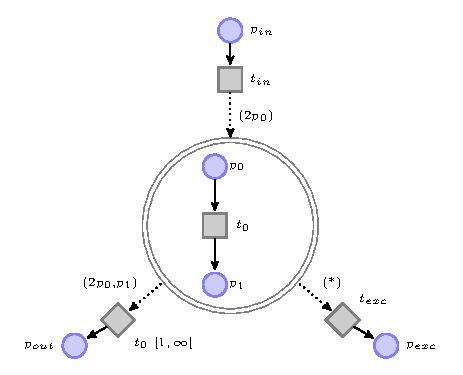
\includegraphics[keepaspectratio,width=.6\textwidth]{macroplace.eps}
  \caption[An SITPN model with a macroplace.]{The macroplace is the
    double-lined circle that encapsulates an SITPN subnet; the subnet
    is called a \textit{refinement}. The arcs that enter and go out of
    the macroplace are particular arcs represented by dotted
    arrows. The input (resp. output) arc on top (at the bottom left)
    of the macroplace is a called an input (resp. output) situation
    arc. The arc at the bottom right of the macroplace is called an
    \emph{exception} arc.}
  \label{fig:macroplace}
\end{figure}

The formal definition of the SITPN structure with macroplaces and its
formal semantics have been described in \cite{Leroux2014}. Adding
macroplaces to the actual SITPN structure will impact the
transformation function, and all the surrounding proofs. Moreover, a
macroplace is connected to an exception arc that comes with an
asynchronous firing semantics. The mixing of asynchronous and
synchronous semantics in the formal semantics of SITPNs with
macroplaces will add new challenges in terms of formalization and
proofs.

In the actual semantics of SITPNs, we considered that only one clock
signal regulated the evolution of the system. However, the formalism
of the \hilecop{} high-level models includes the possibility to assign
different clock \textit{domains} to different parts of the same input
model. Thus, the modeled system is qualified as a multi-clock domain
system. It means that the different parts of the system are not
evolving at the same pace. Therefore, a mechanism of
\textit{asynchronous} message sending relates two parts with different
clock domains, and allows these parts to communicate together. The
system corresponds to a Globally Asynchronous Locally Synchronous
(GALS) architecture.  The semantics of SITPNs that integrate
multi-clock domains has not been formalized yet. The multi-clock
domain aspect also implies modifying the \hvhdl{} semantics to
integrate multiple clock signals in the simulation loop.

% The \coq{} proof assistant provides a way to extract \ocaml{} or
% \textsf{Haskell} code from a \coq{} function. Thus, proving that our
% \coq{} implementation of the \hilecop{} model-to-text transformation
% is semantic preserving would allow us to extract a sound \ocaml{} or
% \textsf{Haskell} program out of it. This program could then replace
% the existing \textsf{Java} implementation of the \hilecop{}
% methodology. At least, the engineers in charge of maintaining the
% current \hilecop{} implementation are open to the idea. However, in
% the certification standards of safety-critical software programs, the
% executed code may not be the one over which the formal verification
% has been conducted (e.g. EAL 7 in the Common Criterion standard).

The question of how much our actual execution semantics and proofs
will adapt to the addition of these new elements is still
open. Moreover, the question of how to parameterize our execution
semantics and transformation function in order to anticipate these
changes is also an interesting question regarding the field of proof
engineering.

All the programming tasks described in this article have been
performed within the framework of the \coq{} proof assistant. The
produced code is fully accessible under the following \textsf{Git}
repository:

\begin{center}
  \url{https://github.com/viampietro/ver-hilecop}
\end{center}

% \section{Introduction}
\label{sec:intro}

The domain of Model-Based Systems Engineering (MBSE) \cite{Long2011}
proposes a framework to help engineers to design and produce digital
systems, in a well-documented, safe and reliable way. Comparable to
what Model Driven Engineering (MDE) does in the world of software
engineering, models are first order concepts in MBSE.  As illustrated
in Figure~\ref{fig:MBSE-ps}, a MBSE process describes a way to design
a digital system starting from a high-level view of the system. This
high-level view can follow a graphical formalism such as SysML
\cite{Friedenthal2014} or Petri nets (PNs) \cite{Petri1962}, or a
textual one such as SystemC \cite{Black2009} or VHDL
\cite{Ashenden2010}. Then, the MBSE process describes many refinements
phases (the downward-going green arrows in Figure~\ref{fig:MBSE-ps})
during which the input model will be transformed; at each refinement
phase, the model goes down in abstraction towards its final
implementation as a hardware circuit. A refinement phase, which is
also a transformation phase, can be performed automatically or
manually.

\begin{figure}[H] \centering
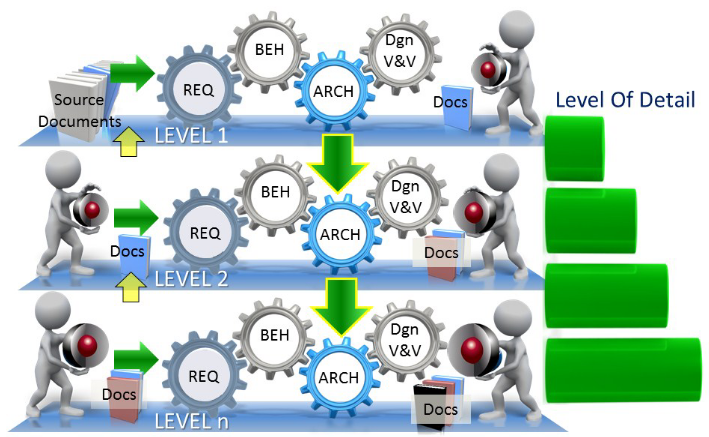
\includegraphics[keepaspectratio,width=.7\textwidth]{MBSE-ps.png}
  \caption[A Model-Based Systems Engineering process.]{A Model-Based
Systems Engineering process; REQ stands for requirements, BEH for
behavior, ARCH for architecture, Dgn V\&V for design verification and
validation. This figure is an excerpt from \cite{Long2011}.}
  \label{fig:MBSE-ps}
\end{figure}

In the case where the digital system being designed is a
safety-critical system, an MBSE process will often employ formal
models as the design formalism. Thus, these models enable a certain
extent of mathematical reasoning to prove that safety properties are
met during the design V\&V phase (cf. Figure~\ref{fig:MBSE-ps}).

To assist the engineers in the design and the implementation of
safety-critical digital systems, the CAMIN team came up with a process
called the ``\hilecop{} methodology'' \cite{Andreu2009}.  This
methodology follows the principles of a MBSE process and relies on
several transformations going from abstract models to concrete FPGA
(Field-Programmable Gate Array) or ASIC (Application-Specific
Integrated Circuit) implementations through the production of VHDL
code. Figure~\ref{fig:hilecop-wf} details the global workflow of
\hilecop{}.

\begin{figure}[H]
\centering
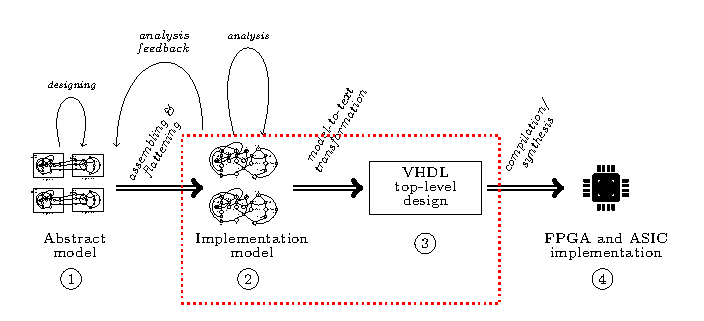
\includegraphics[keepaspectratio=true,width=\textwidth]{hilecop-wf.eps}
\caption[Workflow of the \hilecop{} methodology.]{Workflow of the
  \hilecop{} methodology; horizontal double arrows indicate the
  transformation phases, i.e. the refinement phases in MBSE terms;
  simple arrows indicate different kinds of operations performed at a
  given step.}
\label{fig:hilecop-wf}
\end{figure}

In Figure~\ref{fig:hilecop-wf}, Step~1 corresponds to the design phase
of a digital system. At this step, the user produces a model of the
required system; the leveraged model formalism is a graphical
formalism based on component diagrams and specific Petri nets (PNs).
In Figure~\ref{fig:hilecop-wf}, the transformation from Step~1 to
Step~2 flattens the model. The internal behaviors of separate
components are connected according to the interface compositions, and
embedding component structures are removed. The result of this
transformation step is a global PN that represents the internal
behavior of the digital system.  The class of PNs used in \hilecop{}
has been specifically devised for the design of safety-critical
digital systems; a first thesis has formalized the execution semantics
of these PN models \cite{Leroux2014}. % What makes them a very
% particular kind of models is their \textit{synchronous} execution
% semantics. This semantics denotes from the standard
% \textit{asynchronous} execution of PNs.
Due to its mathematical
foundations, a PN model can be analyzed, and a proof that a given
model meets some properties can be automatically produced through the
direct analysis of the structure or through the use of model-checking
techniques. This feature of PNs has been one of the reason of the
adoption of this formalism as \hilecop{}'s base formalism. A thesis
has been dedicated to the development of new methods to analyze the
\hilecop{} PN models \cite{Merzoug2018}. The analysis phase is here to
convince the engineers that they are indeed designing a safe
system. The analysis process is a round trip between Step~1 and
Step~2.  It aims at producing a model that is conflict-free (see
Section~\ref{sec:hilecop-models} for more details about the definition
of a conflict), bounded, and deadlock-free, using model-checking
techniques.  After several iterations, the model should reach
soundness and is then said to be \emph{implementation-ready}.

In Figure~\ref{fig:hilecop-wf}, from Step~2 to Step~3, \vhdl{} source
code is then generated by means of an automatic model-to-text
transformation. The generated code describes a \vhdl{} design, i.e. a
textual description of a hardware system, which has an interface
defining input and output ports and an internal behavior called an
architecture.

From Step~3 to Step~4, the \vhdl{} compilation/synthesis and the FPGA
programming, or ASIC realization, are finally performed using
industrial tools. At the end of Step~4, the designed circuit is
physically built on an FPGA device or an ASIC.  What happens between
Step~3 and Step~4 appears as a black box in the whole \hilecop{}
methodology. Therefore, we will not consider this transformation
phase, which will not be verified.

\subsection{Verifying the \hilecop{} methodology}
\label{sec:verif-hilecop}

The use of Petri nets as a base model is one of the major advantage of
the \hilecop{} methodology. All the analysis tools that accompany the
Petri net formalism, and allow us to prove that the models meet some
required properties, qualify the \hilecop{} methodology as a formal
method for the design and implementation of safety-critical digital
systems. However, the advantages provided by the use Petri nets would
be lost if one of the transformations performed during the process
changes the input model in a way that would alter its behavior. Thus,
the engineers would have specified a perfectly correct digital system
but would never obtain the expected circuit on a physical device. In
order to reinforce the confidence in the \hilecop{} methodology, the
goal of our work is to verify, by establishing a formal proof, that
the model-to-text transformation from Step~2 to Step~3 (i.e. the
framed part with red dotted lines in Figure~\ref{fig:hilecop-wf})
preserves the behavior of the input models into the generated \vhdl{}
designs. We choose to carry out this task as a deductive verification
task.  We aim at proving a theorem stating that the \hilecop{}
model-to-text transformation is \textit{semantic-preserving}. This
theorem will be of the following form: for all PN model, input to the
\hilecop{} transformation, the generated output \vhdl{} design behaves
similarly at execution time. Section~\ref{sec:proof} formally presents
our behavior preservation theorem, and thus, what we mean about the
similarity of execution between a PN model and a \vhdl{} design.

One could argue that to qualify the entire \hilecop{} methodology, one
has to verify all the transformations used in the methodology,
i.e. consider also the transformation from Step~1 to Step~2, and the
transformation from Step~3 to Step~4. However, we shall say that:

\begin{itemize}
\item The transformation from Step~1 to Step~2 changes the structure
  of the component-based input model. Even if the removal of the
  component structures induces some structural rearrangements, the
  behavior of the flattened model is almost similar to the one of the
  component-based model. Therefore, we argue that verifying that this
  transformation is semantic-preser\-ving is an easy enough task.

\item The transformation from Step~3 to Step~4 is performed by
  industrial tools. We rely on these tools because they are widely
  used in the industry for the development of safety-critical systems
  (e.g. cadence tools in aerospace and defense domains). Moreover, the
  compiler/synthesizer used at this stage of the methodology is a
  proprietary product. Thus, we don't have any access to the code of
  this program. % Moreover, the compiler/synthesizer performs a lot of
  % optimizations over the input \vhdl{} code. Even with a provided
  % access to the code, verifying such an optimizing compiler would not
  % possible within the time-span of this thesis.
\end{itemize}

% Now that we have clarified the nature of the verification task we want
% to achieve, we can state our research question as follows:

% \begin{center}
%   \textsc{Can we prove that the model-to-text transformation described
%     in the \hilecop{} methodology is semantic preserving?}
% \end{center}

\subsection{Related work}
\label{sec:related-work}

The verification task we want to achieve is really close to the formal
verification of compilers for programming languages. Compiler
verification has been widely explored, and many works are accessible
in the literature \cite{Dave2003}. The major source of inspiration of
this work has been the work done on the \ccert{} certified C compiler
\cite{Leroy2009}. Thus, we argue here that the scientific interest of
our research comes from the comparison between the methods used to
perform our verification task and the methods used to perform similar
verification task in other domains such as compiler verification. The
following research questions arises:

\begin{itemize}
\item What are the similarities and the differences between the
  \hilecop{} transformation and other transformation situations
  (compilers, model transformations\dots)?
\item Is there a strategy to perform the verification of the
  \hilecop{} transformation?
\item How far the correspondence holds between this strategy and the
  strategy used in other transformation situations such as compiler
  verification?
\end{itemize}

To achieve the formal verification of \hilecop{}, our approach is
similar to what has been done for the \ccert{} compiler. The idea is
to formalize the semantics of the source and target languages, and
verify that the transformation preserves the semantics of any input
model. In the thesis, we propose both to perform the formalization
work on ``paper'' and mechanize it within the \coq{} proof assistant
\cite{Bertot2004}.

In the case of \hilecop{}, some specificities of the source and target
languages introduce additional technical difficulties in the process
of formal verification. A first difference pertains to \hilecop{}'s
high-level formalism (the input language), which is quite
abstract. This formalism depends on PNs, and thus is not a common
programming language.

A second difference is about the \vhdl{} language (the output
language).  Similarly to the PN models used in \hilecop{}, the \vhdl{}
language is not a common programming language as its purpose is both
the structural and behavioral description of hardware
circuits. % Although previous work has been conducted toward the
% formalization of the \vhdl{} semantics \cite{Kloos2012}, a semantics
% that is able to both handle all the constructs in the generated
% programs, and facilitate the proof of behavior preservation, still
% needs to be designed.

\todo[inline]{ Here put the literature review.}

To further motivate the necessity of the verification task, the
development of neuroprostheses by the INRIA CAMIN team is at the base
of the creation of the Neurrinov
company\footnote{\url{http://neurinnov.com/}}. The Neurrinov company
is now looking towards the industrial development of such
neuroprostheses. We hope that once the verification performed on the
\hilecop{} methodology, it will help to obtain the CE certification,
related to the EU 2017/745 regulation text, necessary to qualify the
neuroprostheses as eligible for the medical market.

Moreover, the \hilecop{} methodology comes with a working
implementation based on the Eclipse framework . This software is
currently used by the engineers of the Neurinnov company to design the
digital systems having a part in safety-critical implantable medical
devices.

To the purpose of formal verification, we will implement the
\hilecop{} model-to-text transformation leveraging the functional
language of the \coq{} proof assistant. However, after the
mechanization of the proof of semantic preservation, we could use the
extraction feature of the \coq{} proof assistant to produce the
implemented transformation as an \ocaml{} program. Then, we will be
able to connect this program to the existing \hilecop{} software in
order
to use the verified version of the transformation.\\

This article is structured as
follows. Section~\ref{sec:hilecop-models} presents the specific kind
of Petri net models which are the input models of \hilecop{}'s
model-to-text transformation.  Section~\ref{sec:hvhdl} gives a formal
definition of the syntax and semantics of a subset of the \vhdl{}
language that we call \hvhdl{}. \hvhdl{} is the target language of the
programs generated by \hilecop{}'s model-to-text transformation.
Section~\ref{sec:m2t} presents the algorithm of the transformation and
its implementation with the \coq{} proof assistant.
Section~\ref{sec:proof} details the semantic preservation theorem
expressing that the \hilecop{} transformation is semantic-preserving.
It also gives the high-level theorems and lemmas involved in the proof
of the semantic preservation theorem.  Finally,
Section~\ref{sec:concl} ends the article, and outlines the
perspectives regarding the full completion of the task of proving that
the \hilecop{} transformation is semantic-preserving.

% \section{Models of digital systems in \hilecop{}}
\label{sec:hilecop-models}

Let us introduce the input formalism of \hilecop{}'s model-to-text
transformation: Synchronously executed, extended, generalized,
Interpreted Time Petri Nets with priorities (SITPNs). The
formalization of the SITPN structure and semantics is mainly the
result of two Ph.D. theses \cite{Leroux2014,Merzoug2018}. We made a
preciser definition of both the SITPN structure and its semantics, as
precision is needed for proving semantic preservation. We have
implemented both structure and semantics in
\coq{}\footnote{\url{https://github.com/viampietro/ver-hilecop/tree/master/sitpn}}. Moreover,
we added complementary definitions, concerning the well-definition of
an SITPN input model, that are required to express our semantic
preservation theorem. In this section, we assume that the reader has
some knowledge of the Petri net formalism and its semantics, so that
words like firing, or marking, need no explanation. For more
information on the topic of Petri nets, the reader can refer to
\cite{David1994}, \cite{Murata1989}, or \cite{Diaz2001}.

\begin{figure}[H]
\centering
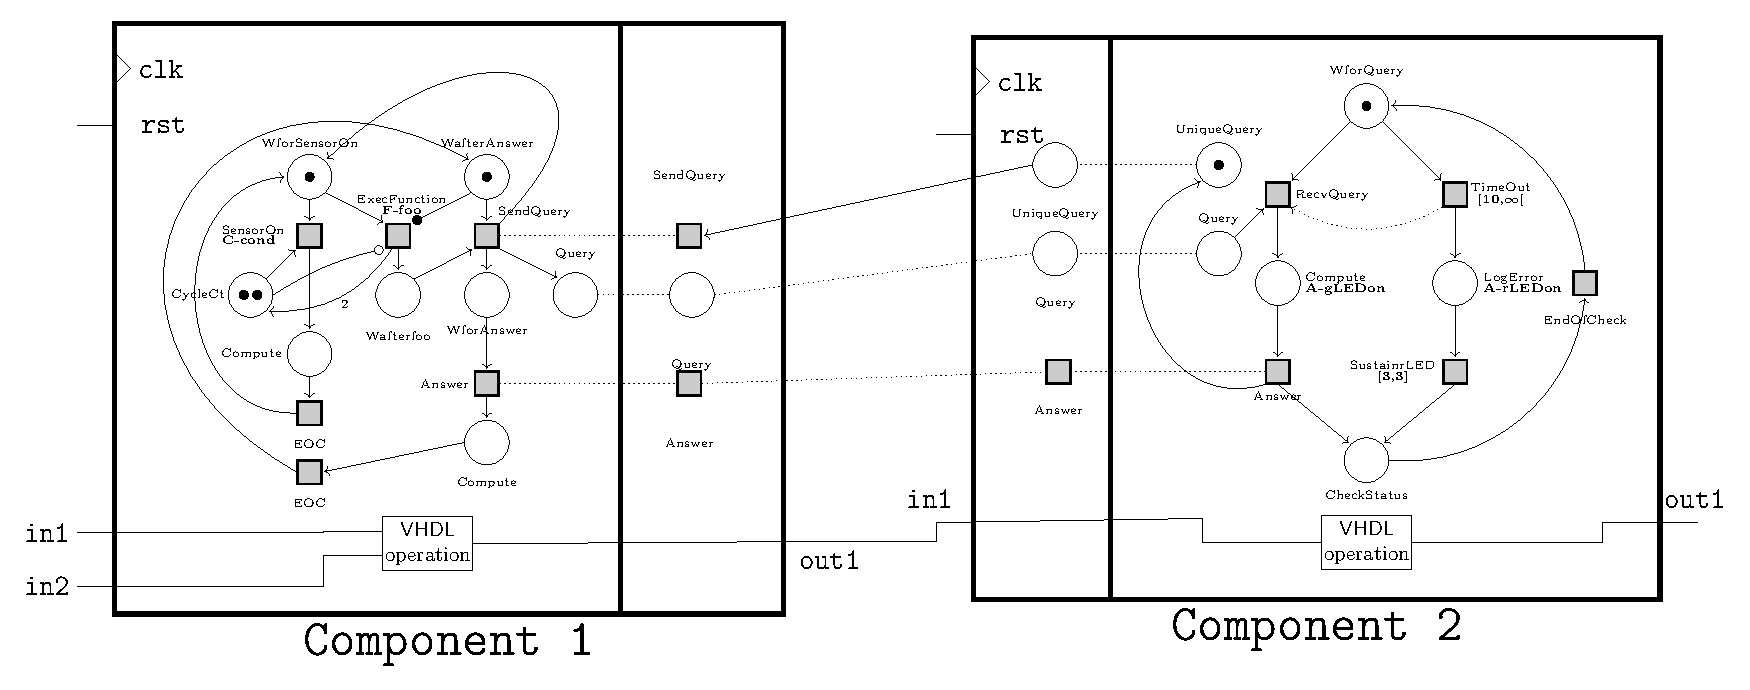
\includegraphics[keepaspectratio=true,width=\textwidth]{abs-model.eps}
\caption[An example of model of digital system in \hilecop{}.]{A
  component-based model of digital system in \hilecop{}.}
\label{fig:abs-model}
\end{figure}

In \hilecop{}'s high-level formalism, a model of digital system is
composed of boxes that represent the different components of the
system. Figure~\ref{fig:abs-model} gives an example of such a model.
The internal behavior of each component is defined by a SITPN model.
The elements of a component's internal behavior can be connected to
the elements of another component's behavior through an interface. Two
elements are either connected through a place-transition (or
transition-place) arc, or through a fusion arc (dotted line in
Figure~\ref{fig:abs-model}). While designing a component, an engineer
can also define input and output ports in the component interface,
declare internal signals, and perform operations over the ports and
internal signals by writing \vhdl{} code. All the \vhdl{} code defined
in this way will be copied as is in the output \vhdl{} design during
the model-to-text transformation. Note that all components declare a
clock and a reset signal (cf. \texttt{clk} and \texttt{rst} in
Figure~\ref{fig:abs-model}). These signals are related to the
synchronous execution of the system in the final physical device.

Before being transformed into \vhdl{} code, the model is flattened
down (cf. Step \circled{1} to step \circled{2} in
Figure~\ref{fig:hilecop-wf}). All component structures are removed,
and the result is one global SITPN model. During this flattening step,
all elements that were connected through fusion arcs are merged
together. Figure~\ref{fig:impl-model} presents the global SITPN model
resulting from the flattening of the component-based model of
Figure~\ref{fig:abs-model}.

\begin{figure}[H]
\centering
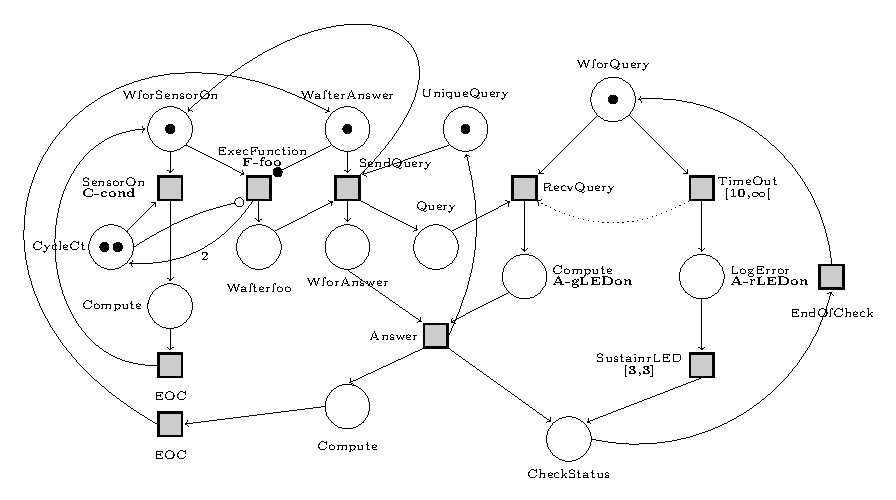
\includegraphics[keepaspectratio=true,width=\textwidth] {impl-model.eps}
\caption[Global Petri net model.]{A global Petri net model obtained
  after the flattening of a \hilecop{} high-level model.}
\label{fig:impl-model}
\end{figure}

SITPNs are a combination of multiple classes of PNs, namely: extended
PNs, generalized PNs, interpreted PNs, time PNs and PNs with
priorities. A generalized Petri net admits the weight of its arcs to
be a natural number instead of the default value of one (i.e. when no
number is written above the arc). An extended Petri net introduces two
kind of place-transition arcs, the \textit{inhibitor} arc,
characterized by a white circle head, and the \textit{test} arc, which
has a black circle head. These arcs add conditions the firing of a
connected transition, however, they do not cause tokens to be removed
from input places at firing time. In Figure~\ref{fig:impl-model}, the
arc from place CycleCt to transition ExecFunction is an inhibitor arc,
and the arc from place WafterAnswer to ExecFunction is a test arc.
Now, let us introduce more specifically the class of interpreted PNs,
time PNs and PNs with priorities.

\paragraph{Interpreted Petri nets (IPNs)}
% As stated in \cite{David1994}, Interpreted Petri Nets (IPN) ``can be
% applied to various interpretations according to the use wished to be
% made of it''.
In its general definition \cite{David1994}, an IPN is associated with
a finite set of variables $V$, a finite set of operations $O$, and a
finite set of conditions $C$. Operations of the $O$ set are associated
with places and triggered when the places become marked. The execution
of operations affects the value of the variables, and the value of
conditions depends on Boolean expressions computed upon the variables.
Conditions are associated with transitions and become involved in the
firing process.  In the \hilecop{} version of
IPNs, % refines the concepts of the general
% definition. In this version, 
the set of variables corresponds to the set of \vhdl{} signals that
are handled by the model; a signal can be an input port, an output
port or an internal signal of the modeled hardware circuit. The
operations, implemented by \vhdl{} procedures, are separated in two
kinds, namely: actions and functions. Actions (or continuous
operations) are associated to the places; all the actions associated
to a place $p$ are activated as long as $p$ is marked (i.e. as long as
$p$ holds a token). Functions (or discrete operations) are associated
to the transitions; when a transition $t$ is fired, all functions
associated to $t$ are executed once. In Figure \ref{fig:impl-model},
\textbf{C-cond} is a condition associated to the transition SensorOn;
\textbf{F-foo} is a function associated to the transition
ExecFunction; \textbf{A-gLEDon} and \textbf{A-rLEDon} are two actions
associated to the Compute and LogError places.

\paragraph{Time Petri nets (TPNs)}

In a TPN, time intervals can be associated to transitions, along with
a dynamic time counter value. Thus, the firing of a transition must
happen in a certain time window. In the \hilecop{} version of TPNs,
time intervals are of the form $[a, b]$, where $a\in\mathbb{N}^{*}$
and $b\in\mathbb{N}^{*}\sqcup\{\infty\}$.  In
Figure~\ref{fig:impl-model}, transitions SustainrLED and TimeOut are
both associated with time intervals.

\paragraph{Petri nets with priorities}

Two transitions are in structural conflict if they have a common input
place connected through a \textit{basic} arc (i.e. neither inhibitor
nor test arc). When two transitions in structural conflict are firable
at the same time and if the firing of one of the transitions disables
the other, then, the conflict becomes \textit{effective}. In a Petri
net with priorities, it is possible to specify a firing priority in
the case where the conflict between two transitions becomes
effective. In that case, the transition with the highest firing
priority will always be fired first. In Figure \ref{fig:impl-model},
the fact that transition TimeOut has a higher firing priority than
transition RecvQuery is graphically represented by a dotted arrow. \\

\noindent{}Now let us formally introduce the structure of SITPNs:

\begin{definition}[SITPN]
  \label{def:sitpn}
  A synchronously executed, extended, generalized, interpreted, and
  time Petri net with priorities is a tuple
  ${<}P,T,pre,post,M_0,{\succ},\mathcal{A},\mathcal{C},\mathcal{F},
  \mathbb{A},\mathbb{C},\mathbb{F},{I_s}{>}$, where we have:
  % 
  \begin{enumerate}
  \item $P=\{p_0,\ldots,p_n\}$, a finite set of places.
  \item $T=\{t_0,\ldots,t_m\}$, a finite set of transitions.
  \item
    $pre\in{}P\rightarrow{}T\nrightarrow(\mathbb{N}^{*}\times\{\mathtt{basic},\mathtt{inhib},\mathtt{test}\})$,
    the function associating a weight and a type to place-transition
    edges.
  \item $post\in{}T\rightarrow{}P\nrightarrow\mathbb{N}^{*}$, the
    function associating a weight to transition-place edges.
  \item $M_0\in{}P\rightarrow\mathbb{N}$, the initial marking of the SITPN.
  \item $\succ\subseteq{}(T\times{}T)$, the priority relation, which
    is a strict partial order over the set of transitions.
  \item $\mathcal{A}=\{a_0,\ldots,a_i\}$, a finite set of continuous actions.
  \item $\mathcal{F}=\{f_0,\ldots,f_k\}$, a finite set of functions.
  \item $\mathcal{C}=\{c_0,\ldots,c_j\}$, a finite set of conditions.
  \item $\mathbb{A}$ $\in$ ${}P$ $\rightarrow$ $\mathcal{A}$
    $\rightarrow$ $\mathbb{B}$, the function associating actions to
    places.  $\forall{}p\in{}P$, $\forall{}a\in\mathcal{A}$,
    $\mathbb{A}(p,a)=\mathtt{true}$, if $a$ is associated to $p$,
    $\mathbb{A}(p,a)=\mathtt{false}$ otherwise.
  \item $\mathbb{F}\in{}T\rightarrow\mathcal{F}\rightarrow\mathbb{B}$,
    the function associating functions to transitions.
    $\forall{}t\in{}T,~\forall{}f\in\mathcal{F},$
    $\mathbb{F}(t,f)=\mathtt{true}$, if $f$ is associated to $t$,
    $\mathbb{F}(t,f)=\mathtt{false}$ otherwise.
    
  \item $\mathbb{C} \in T \rightarrow \mathcal{C} \rightarrow\{-1,0,1\}$, the
    function associating conditions to transitions.
    $\forall t \in T$, $\forall c \in \mathcal{C}$,
    $\mathbb{C}(t,c)=1$, if $c$ is associated to $t$,
    $\mathbb{C}(t,c)=-1$, if $\bar{c}$ is associated to $t$,
    $\mathbb{C}(t,c)=0$ otherwise.
  \item
    $I_s\in{}T\nrightarrow(\mathbb{N}^{*}\times(\mathbb{N^{*}}\sqcup\{\infty\}))$,
    the partial function associating time intervals to transitions.
  \end{enumerate}
\end{definition}

In Definition~\ref{def:sitpn}, we do not consider the set of \vhdl{}
signals manipulated by a SITPN model. As a consequence, the structure
holds neither the association between conditions and Boolean
expressions, and nor the association between actions/functions and
operations (i.e. \vhdl{} procedures that act upon signal values).  In
this simplified version of the SITPN structure, conditions, actions
and functions are only considered as finite sets of indexed elements
associated with the places and transitions of a SITPN.

\subsection{Synchronous execution semantics}
\label{subsec:hpn-particularities}

The SITPN semantics describes the evolution of the state of a SITPN
through a given number of clock cycles; thus, we must first define the
SITPN state structure. In what follows, for a given $sitpn\in{}SITPN$,
$T_i$ denotes the definition domain of $I_s$, i.e. the set of
transitions associated with a time interval, referred to as
\textit{time transitions}.

\begin{definition}[SITPN State]
  \label{def:sitpnstate}
  For a given $sitpn\in{}SITPN$, let $S(sitpn)$ be the set of possible
  states of $sitpn$. An SITPN state $s\in{}S(sitpn)$ is a tuple
  ${<}M,I,reset_t,ex,cond{>}$, where:
  \begin{enumerate}
  \item $M\in{}P\rightarrow\mathbb{N}$ is the current marking of
    $sitpn$.
  \item\label{item:sitpn-state-tc} $I\in{}T_i{}\rightarrow\mathbb{N}$
    is the function mapping time transitions to their current time
    counter value.
  \item\label{item:sitpn-state-rst}
    $reset_t\in{}T_i\rightarrow\mathbb{B}$ is the function mapping
    time transitions to time counter reset orders (defined as
    Booleans).
  \item $ex\in{}\mathcal{A}\sqcup\mathcal{F}\rightarrow\mathbb{B}$ is
    the function representing the current activation (resp. execution)
    state of actions (resp. functions).
  \item $cond\in\mathcal{C}\rightarrow\mathbb{B}$ is the function representing the
    current value of conditions (defined as Booleans).
  \end{enumerate}
\end{definition}

As described in Definition~\ref{def:sitpnstate}, the state of a SITPN
is characterized by its marking, the value of time counters, the reset
orders assigned to time counters, the execution/activation status of
actions/functions (Boolean values), and the value of conditions (also
Boolean). Regarding actions and functions, note that we are only
interested in the fact that a given action/function is
activated/executed but no more in actually executing the associated
operation.\\

Before describing the SITPN state transition relation, we need to
formally define the sensitization of a given transition by a given
marking, and the firability of a given transition with respect to a
given SITPN state.

\begin{definition}[Sensitization]
  \label{def:sens}
  A transition $t\in{}T$ is said to be sensitized, or enabled, by a
  marking $M$, which is noted $t\in{}Sens(M)$, if
  $\forall{}p\in{}P,\forall\omega\in\mathbb{N}^{*},~\big(pre(p,t)=(\omega,\mathtt{basic})\vee{}pre(p,t)=(\omega,\mathtt{test})\big)\Rightarrow{}M(p)\ge{}\omega$,
  and $pre(p,t)=(\omega,\mathtt{inhib})\Rightarrow{}M(p)<{}\omega$.
\end{definition}

\begin{definition}[Firability]
  \label{def:firable}
  A transition $t\in{}T$ is said to be firable at a state
  $s={<}M,I,reset_t,ex,cond{>}$, which is noted $t\in{}Firable(s)$, if
  $t\in{}Sens(M)$, and $t\notin{}T_i$ or $I(t)\in{}I_s(t)$, and
  $\forall c \in \mathcal{C}, \mathbb{C}(t, c) = 1 \Rightarrow cond(c)
  = 1$ and $\mathbb{C}(t, c) = -1 \Rightarrow cond(c) = 0$.
\end{definition}


All transitions that are firable at a given state are possible members
of the set of fired transitions. A firable transition is also a fired
transition if it is still enabled by the \textit{residual} marking,
that is, the marking resulting from the firing of transitions with a
higher priority.  Priorities are defined with the priority relation,
which is a part of the SITPN structure.  As illustrated in
Figure~\ref{fig:resid-marking}, to determine which transitions of
$t_0$, $t_1$ and $t_2$ are fired, a \emph{residual marking} is
computed by following the priority order. For each transition of the
group $t_0$, $t_1$ and $t_2$, the residual marking represents the
remaining tokens in $p_0$ after the firing of transitions with a
higher firing priority.  Thus, the recursive definition of the set of
fired transitions at a given SITPN state is as follows:

\begin{definition}[Fired]
  \label{def:fired}
  A transition $t\in{}T$ is said to be fired at the SITPN state
  $s={<}M,I,reset_t,ex,$ $cond{>}$, which is noted $t\in{}Fired(s)$,
  if $t\in{}Firable(s)$ and
  $t\in{}Sens\big(M-\sum\limits_{t_i\in{}Pr(t)}pre(t_i)\big)$, where
  $Pr(t)=\{t_i~|~t_i\succ{}t\wedge{}t_i\in{}Fired(s)\}$.
\end{definition}


\begin{figure}[H]
  \centering
  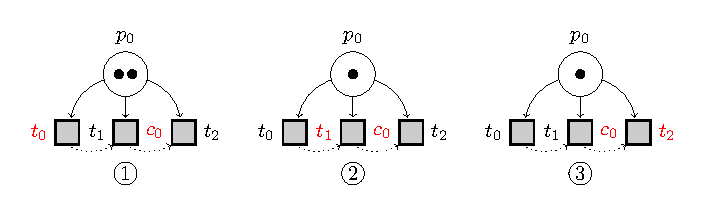
\includegraphics[keepaspectratio=true, width=.8\textwidth]{resid-marking.eps}
  \caption[Computation of the residual marking of a group of
  conflicting transitions.]{Computation of the residual marking for a
    group of conflicting transitions. At \circled{1}
    (resp. \circled{2} and \circled{3}), place $p_0$ holds the
    residual marking for transition $t_0$ (resp. $t_1$ and
    $t_2$). Condition $c_0$ appears in normal font to indicate that
    its current value is \texttt{false}.}
  \label{fig:resid-marking}
\end{figure}

Note that the computation of the residual marking only involves the
consumption phase of the firing process; tokens are withdrawn from
places, but none are generated.

Note also that there is an equivalence between being firable and being
fired at a given state when considering a \textit{top-priority}
transition, i.e. a transition for which there exists no transition
with a higher firing priority.

\paragraph{The state transition relation}

The evolution of the state of a SITPN is \textit{synchronized} with
the rising edge event and the falling edge event of a clock signal.
The rising edge event triggers the marking update, the computation of
time counter reset orders, and the execution of functions. On the
falling edge of the clock signal, the value of conditions are
updated. As the SITPN structure does not hold the link between Boolean
expressions computed over \vhdl{} signals and conditions, the update
of condition values is represented by the injection of fresh Boolean
values coming from an environment. Moreover, the falling edge event
triggers the evolution of the time counter values; values are
incremented, reset, or stalling in the case where a time counter has
reached the upper bound of its associated time interval. Finally, all
actions associated with marked places are
activated. Figure~\ref{fig:sitpn-state-exec} gives an example of the
evolution of the state of a given SITPN through one clock cycle,
happening in the middle of other clock cycles.

\begin{figure}[H]
  \centering
  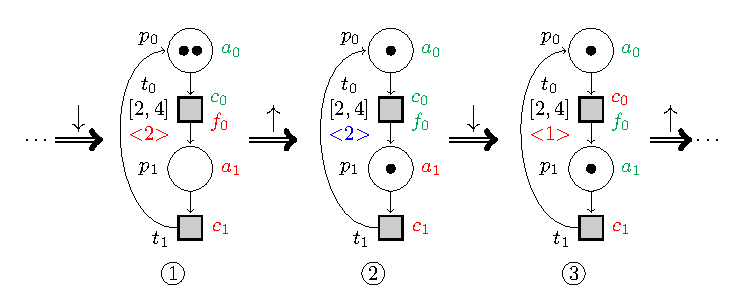
\includegraphics[keepaspectratio=true, width=.8\textwidth]{sitpn-state-evol.eps}
  \caption[Evolution of an SITPN over one clock cycle.]{The evolution
    of a SITPN over one clock cycle. Conditions (i.e. $c_0$ and $c_1$)
    appear in bold font when \texttt{true}; actions (i.e. $a_0$ and
    $a_1$) and functions ($f_0$) appear in bold font when
    activated/executed; time counters appear between diamond brackets,
    and are represented between inverted brackets when they are
    subject to a reset order.}
  \label{fig:sitpn-state-exec}
\end{figure}

In Figure~\ref{fig:sitpn-state-exec}, from Step~1 to Step~2, the
rising edge of the clock signal triggers the firing of transition
$t_0$. As transition $t_0$ is firable and is not in effective conflict
with other transitions, $t_0$ is fired: one token is consumed in place
$p_0$ and one token is produced in place $p_1$. Also, function $f_0$
is executed at the occurrence of the rising edge of the clock signal,
and thus, $f_0$ appears in bold font at Step~2. Consequently to the
firing of $t_0$, a reset order is sent to the time counter of $t_0$,
and it appears between inverted brackets at Step~2. From Step~2 to
Step~3, the falling edge updates the action activation status: $a_0$
stays activated as place $p_0$ is still marked; $a_1$ becomes newly
activated as place $p_1$ just received a token. Time counters are
updated: $t_0$'s time counter is set to zero as the transition
previously received a reset order. However, as $t_0$ is still enabled
by the new marking, its time counter is incremented. Thus, the
resulting time counter value at Step~3 is of one (i.e. result of reset
plus increment). Also, the environment provides a new value to each
condition. As a consequence, condition $c_0$ takes the value
\texttt{false} and condition $c_1$ keeps the same value.

We formalize the evolution of a SITPN state synchronized with the
events of a clock signal with the following state transition relation:

\begin{definition}[SITPN state transition]
  \label{def:semantics}
  For a given $sitpn\in{}SITPN$, the SITPN state transition relation
  $\rightarrow\subseteq{}(\mathbb{N}\rightarrow\mathcal{C}\rightarrow\mathbb{B})\times{}\mathbb{N}\times{}S(sitpn)\times{}\{\uparrow,\downarrow\}\times{}S(sitpn)$
  is noted as follows $E_c,\tau\vdash{}s\xrightarrow{clk}s'$, where
  $E_c\in\mathbb{N}\rightarrow\mathcal{C}\rightarrow\mathbb{B}$ is an
  environment that maps the conditions of $sitpn$ to a Boolean value
  at a given clock count, $\tau\in\mathbb{N}$ is the current clock
  count, $s,s'\in{}S(sitpn)$ are two states of $sitpn$ and
  $clk\in\{\uparrow,\downarrow\}$ is a clock event. The relation is
  defined by the two following rules:
  
  \begin{itemize}
  \item
    $\forall{}E_c\in\mathbb{N}\rightarrow\mathcal{C}\rightarrow\mathbb{B}$,
    $\forall\tau\in\mathbb{N}$, $\forall{}s,s'\in{}S(sitpn)$, we have
    $E_c,\tau\vdash{}s\xrightarrow{\uparrow}s'$, where
    $s=<M,I,reset_t,ex,cond>$ and $s'=<M',I,reset_t',ex',cond>$, if:
    \begin{enumerate}
    \item\label{it:new-marking} $M'$ is the new marking resulting
      from
      the firing of all the transitions contained in $Fired(s)$, i.e.:
      \begin{equation*}
        \forall{}p\in{}P,~M'(p)=M(p)-\sum\limits_{t\in{}Fired(s)}pre(p,t)+\sum\limits_{t\in{}Fired(s)}post(t,p).
      \end{equation*}
      
    \item\label{it:reset-order} A time transition receives a reset
      order if it is fired at state $s$, or, if there exists a place
      $p$ connected to $t$ by a \texttt{basic} or \texttt{test arc}
      and at least one output transition of $p$ is fired and the
      transient marking of $p$ disables $t$; no reset order is sent
      otherwise:
      \begin{equation*}
        \begin{split}
          \forall{}t\in{}T_i,&~t\in{}Fired(s) \\
                             &\lor\big(\exists{}p\in{}P,\omega\in\mathbb{N}^{*}, \\
                             &\quad\quad{}[pre(p,t)=(\omega,\mathtt{basic})\lor{}pre(p,t)=(\omega,\mathtt{test})] \\
                             &\quad\quad\land\sum\limits_{t_i\in{}Fired(s)}pre(p,t_i)>0 \\
                             &\quad\quad\land{}M(p)-\sum\limits_{t_i\in{}Fired(s)}pre(p,t_i)<\omega\big)\\
                             & \Rightarrow{}reset'_t(t)=\mathtt{true}~and~reset'_t(t)=\mathtt{false}~otherwise.  \\
        \end{split}
      \end{equation*}
      
    \item\label{it:exec-fun} All functions associated with at least one fired transition are executed, i.e:
      \begin{equation*}
        \forall{}f\in{}\mathcal{F},~ex'(f)=\sum\limits_{t\in{}Fired(s)}\mathbb{F}(t,f).
      \end{equation*}
    \end{enumerate}
    
  \item
    $\forall{}E_c\in\mathbb{N}\rightarrow\mathcal{C}\rightarrow\mathbb{B}$,
    $\forall\tau\in\mathbb{N}$, $\forall{}s,s'\in{}S(sitpn)$, we have
    $E_c,\tau\vdash{}s\xrightarrow{\downarrow}s'$, where
    $s=<M,I,reset_t,ex,cond>$ and $s'=<M,I',reset_t,ex',cond'>$, if:
    \begin{enumerate}[resume]
    \item\label{it:cond-env} $cond'$ is the function giving the
      (Boolean) values of conditions that are extracted from the
      environment $E_c$ at the clock count
      $\tau$, i.e.:
      \begin{equation*}
        \forall{}c\in{}\mathcal{C},~cond'(c)=E_c(\tau,c).
      \end{equation*}
      
    \item\label{it:activate-actions} All the actions associated
      with at least one
      marked place in the marking $M$ are activated, i.e.:
      \begin{equation*}
        \forall{}a\in{}\mathcal{A},~ex'(a)=\sum\limits_{M(p)>0}\mathbb{A}(p,a).
      \end{equation*}
    \item\label{it:reset-counters} All the time transitions that are
      sensitized by the marking $M$ and received the order to reset
      their time intervals, have their time counter reset and
      incremented, i.e.:
      \begin{equation*}
        \forall{}t\in{}T_i,~t\in{}Sens(M)\land{}reset_t(t)=\mathtt{true}
        \Rightarrow{}I'(t)=1.
      \end{equation*}
      
    \item\label{it:inc-counters} All the time transitions that are
      sensitized by the marking $M$, and
      did not receive a reset order, increment their time counters if time counters are still active, i.e.:
      \begin{equation*}
        \begin{split}
          \forall{}t\in{}T_i,~&t\in{}Sens(M)\land{}reset_t(t)=\mathtt{false}\land{}[I(t)\le{}u(I_s(t))\lor{}u(I_s(t))=\infty]\\
                              & \Rightarrow{}I'(t)=I(t)+1. \\
        \end{split}
      \end{equation*}
    \item\label{it:locked-counters} All the time transitions
      verifying the same
      conditions as above, but with locked counters, keep having locked counters (values are stalling), i.e.:        
      \begin{equation*}
        \begin{split}
          \forall{}t\in{}T_i,~&t\in{}Sens(M)\land{}reset_t(t)=\mathtt{false}\land{}I(t)>{}u(I_s(t))\land{}u(I_s(t))\neq\infty\\
                              & \Rightarrow{}I'(t)=I(t).\\
        \end{split}
      \end{equation*}
      
    \item\label{it:reset-not-sens} All the time transitions disabled by the marking $M$ have their time counters set to zero, i.e.:
      \begin{equation*}
        \forall{}t\in{}T_i,~t\notin{}Sens(M)\Rightarrow{}I'(t)=0.
      \end{equation*}
    \end{enumerate}
    
  \end{itemize}
\end{definition}

Premises~\ref{it:new-marking} to \ref{it:exec-fun} describe the SITPN
state evolution at the rising edge of the clock signal.
Premise~\ref{it:new-marking} corresponds to the marking update. The
computation of the new marking uses the set of fired transitions at
state $s$, i.e. $Fired(s)$. Premise~\ref{it:exec-fun} deals with the
update of the function execution status. Premise~\ref{it:reset-order}
computes the reset orders for time transitions. There are two cases
where a time transition receives the order to reset its time
counter. First, if the transition is one of the fired transitions at
state $s$, then its time counter must be reset on the next falling
edge. Second, if the transition is disabled in a \emph{transient}
manner, then its time counter must also be reset.

Premises~\ref{it:cond-env} to \ref{it:reset-not-sens} describe the
SITPN state evolution at the falling edge of the clock
signal. Premises~\ref{it:cond-env} and \ref{it:activate-actions} deal
with the update of condition values and the activation status of
actions. Note that in Premise~\ref{it:activate-actions} (and also in
Premise~\ref{it:exec-fun}), the sum expression corresponds to the
Boolean sum expression, i.e. the application of the \texttt{or}
operator over the elements of the iterated
set. Premises~\ref{it:reset-counters}, \ref{it:inc-counters},
\ref{it:locked-counters} and \ref{it:reset-not-sens} focus on the
update of time counter values.  In Premise~\ref{it:inc-counters} of
the SITPN semantics, the \emph{active} time counters refer to the time
counters that have not yet overreached the upper bound of their
associated time interval. Of course, a time counter is always active
when the upper bound is infinite. In Premise~\ref{it:locked-counters},
the \emph{locked} time counters refer to the time counters that have
overreached the upper bound of their associated time interval. Of
course, time counters can never be locked in the presence of an
infinite upper bound. In Premises~\ref{it:inc-counters} and
\ref{it:locked-counters}, for a given time interval $i$, $u(i)$
denotes the upper bound of the time interval, and $l(i)$ denotes the
lower bound of the time interval.\\

To give a small-step execution semantics to a SITPN model, we have
defined an execution relation that binds a given SITPN model to an
execution trace, i.e. a time-ordered list of states. The execution
trace is built for a given number of clock cycles, starting from the
initial state of the SITPN model. The execution relation is
implemented in \coq{} by the \texttt{SitpnFullExec} inductive
type\footnote{\url{https://github.com/viampietro/ver-hilecop/blob/master/sitpn/SitpnSemantics.v}}. The
initial state of a SITPN model is formally defined as follows:

\begin{definition}[Initial state]
  \label{def:sitpn-init-state}
  For a given $sitpn\in{}SITPN$, $s_0\in{}S(sitpn)$ is the initial
  state of $sitpn$, such that
  $s_0=<M_0,O_\mathbb{N},O_\mathbb{B},O_\mathbb{B},O_\mathbb{B}>$,
  where $M_0$ is the initial marking of the SITPN, $O_\mathbb{N}$ is a
  function that always returns 0, $O_\mathbb{B}$ is a function that
  always returns \texttt{false}.
\end{definition}

\subsection{Well-definition of a SITPN}
\label{sec:sitpn-wd}

The synchronous execution semantics of SITPNs implies that all
transitions are fired at the same time. In
Figure~\ref{fig:double-consum}, transitions $t_0$ and $t_1$ are both
firable before the rising edge event. As no priority relation is drawn
between the two conflicting transitions, they are both fired at the
occurrence of the event. The system acts as if two tokens were
available in place $p_0$, one for the firing of $t_0$ and another for
the firing of $t_1$.

\begin{figure}[H]
  \centering
  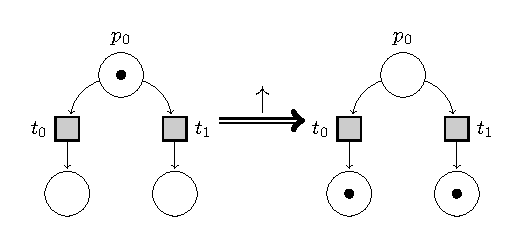
\includegraphics[keepaspectratio=true, width=.5\textwidth]{double-consum.eps}
  \caption[Double consumption of token in a SITPN.]{Double consumption
    of one token in a SITPN. On the left side, the current marking
    before the firing of $t_0$ and $t_1$; on the right side, the
    marking resulting of the firing of $t_0$ and $t_1$. The arrow
    indicates the occurrence of a rising edge that triggers the firing
    process.}
  \label{fig:double-consum}
\end{figure}

In the context of a SITPN, a branching like the one of
Figure~\ref{fig:double-consum}, normally interpreted as a disjunctive
branching, takes the semantics of a conjunctive branching if no
priority are specified between the conflicting transitions. To avoid
the phenomenon of ``double consumption'' of tokens, we enforce the
resolution of any structural conflict by means of mutual exclusion or
through the application of priorities. This policy about the
resolution of structural conflicts is part of the definition of a
\emph{well-defined} SITPN. We must be able to decide which transition
in a conflicting pair will be fired when the conflict becomes
effective. Thus, we give place-centered definition of a group of
transitions in conflict:

\begin{definition}[Conflicting group of transitions]
  \label{def:cgroup}
  For a given $sitpn\in{}SITPN$, the conflicting transitions of a
  given place $p$, noted $conflict(p)$, are all transitions related to
  $p$ with a \texttt{basic} place-transition arc,
  i.e.
  $conflict(p)=\{t\in{}T~\vert~\exists{}\omega\in\mathbb{N}^{*},~pre(p,t)=(\omega,\mathtt{basic})\}$.
\end{definition}

This view of a conflict group reflects the place-centered view of
conflicts as implemented in the \vhdl{} code generated by the
model-to-text transformation.  Figure~\ref{fig:conflict-groups} shows
the conflict group related to place $p_0$ and $p_1$, namely:
$\{t_0,t_3\}$ and $\{t_1,t_4\}$.

\begin{figure}[H]
  \centering
  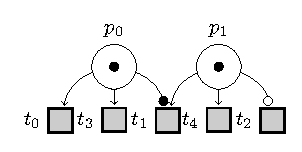
\includegraphics[keepaspectratio,width=.3\linewidth]{conflict-groups.eps}
  \caption[An example of two separate conflict groups.]{An example of
    two separate conflict groups, namely: $\{t_0,t_3\}$ and
    $\{t_1,t_4\}$.}
  \label{fig:conflict-groups}
\end{figure}

In a well-defined SITPN, all conflicts in a conflict group must be
considered, i.e. for all pair of transitions in the group the conflict
must be solved. When the conflict between a pair of transitions
becomes effective, there are two ways to be sure that only one
transition will be fired. The first way is to define a firing order
through a priority relation. The second way is to use a mean of mutual
exclusion. A mean of mutual exclusion ensures that the two transitions
of a conflicting pair will never be firable at the same time. We only
consider two ways of mutual exclusion, namely: mutual exclusion with
complementary conditions and mutual exclusion with inhibitor arcs.

\begin{definition}[Mutual exclusion with complementary conditions]
  \label{def:mutex-conds}
  Given two conflicting transitions $t_0$ and $t_1$, $t_0$ and $t_1$
  are in mutual exclusion with complementary conditions if there
  exists $c\in\mathcal{C}$ such that
  $(\mathbb{C}(t_0,c)=1\land{}\mathbb{C}(t_1,c)=-1)$ or
  $(\mathbb{C}(t_0,c)=-1\land{}\mathbb{C}(t_1,c)=1)$.
\end{definition}

\begin{definition}[Mutual exclusion with an inhibitor arc]
  \label{def:mutex-inhib} Given two conflicting transitions $t_0$ and
  $t_1$, $t_0$ and $t_1$ are in mutual exclusion with an inhibitor arc
  if there exists $p\in{}P$ and $\omega\in{}\mathbb{N}^{*}$ such that
  $(pre(p,t_0)=(\omega,\mathtt{basic})\lor{}pre(p,t_0)=(\omega,\mathtt{test}))\land{}pre(p,t_1)=(\omega,\mathtt{inhib})$
  or
  $(pre(p,t_1)=(\omega,\mathtt{basic})\lor{}pre(p,t_1)=(\omega,\mathtt{test}))\land{}pre(p,t_0)=(\omega,\mathtt{inhib})$.
\end{definition}

Figure~\ref{fig:mutex} illustrates the two means of mutual exclusion
that can be applied to solve a conflict between two transitions.

\begin{figure}[H]
  \centering
  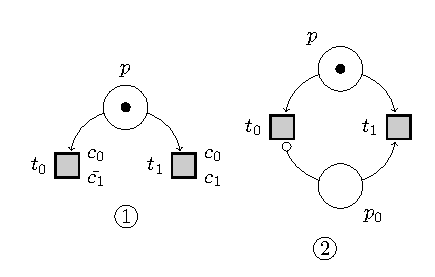
\includegraphics[keepaspectratio,width=.45\linewidth]{mutex.eps}
  \caption[Examples of conflicting transitions in mutual exclusion.]{
    Examples of conflicting transitions in mutual exclusion. At
    \circled{1}, an example of mutual exclusion with complementary
    conditions; at \circled{2}, an example of mutual exclusion with an
    inhibitor arc.}
  \label{fig:mutex}
\end{figure}

In Figure~\ref{fig:mutex}, in situation \circled{1}, condition $c_1$
is associated to $t_1$ and the complementary condition is associated
to $t_0$ thus creating the mutual exclusion. In situation \circled{2},
the arcs $(p_0,t_0)$ and $(p_0,t_1)$ ensure the mutual exclusion
between transitions $t_0$ and $t_1$. Note that in the structure of
mutual exclusion with an inhibitor arc, the weight of the inhibitor
arc and of the one of the basic or test arc must be the same;
otherwise, the mutual exclusion is not effective.\\

\noindent{}A well-defined SITPN is defined as follows:

\begin{definition}[Well-defined SITPN]\label{def:wd-sitpn}
  A given $sitpn\in{}SITPN$ is well-defined if:
  \begin{itemize}
  \item $T\neq\emptyset$, the set of transitions is not empty.
  \item $P\neq\emptyset$, the set of places is not empty.
  \item There is no isolated place, i.e. a place that has neither
    input nor output transitions:\\
    $\nexists{}p\in{}P,~input(p)=\emptyset\wedge{}output(p)=\emptyset$,
    where $input(p)$ (resp. $output(p)$) denotes the set of input
    (resp. output) transitions of $p$.
  \item There is no isolated transition, i.e. a transition that has
    neither
    input nor output places:\\
    $\nexists{}t\in{}T,~input(t)=\emptyset\wedge{}output(t)=\emptyset$,
    where $input(t)$ (resp. $output(t)$) denotes the set of input
    (resp. output) places of $t$.
  \item For all conflict group as defined in
    Definition~\ref{def:cgroup}, either all conflicts (i.e. for all
    pair of transitions in the conflict group) are solved by one of
    the mean of mutual exclusion, or, the priority relation is a
    \emph{strict total} order over the transitions of the conflict group.
  \end{itemize}
\end{definition}

If the properties, given in Definition~\ref{def:wd-sitpn}, are not
ensured, they will lead to compile-time errors during the
transformation of a SITPN model into a \vhdl{} design.


%%% Local Variables:
%%% mode: latex
%%% TeX-master: "main"
%%% End:

% \section{A target language: \hvhdl{}}
\label{sec:hvhdl}

The \hilecop{} model-to-text transformation generates a \vhdl{}
\emph{design} out of an input SITPN model.  \vhdl{} is a hardware
description language. A design represents the highest entity level
that can be described in \vhdl{}. A design defines an interface
(i.e. ports and dimensioning constants), and internal behavior
(i.e. the design architecture). The \vhdl{} Language Reference Manual
(LRM)\cite{VHDL2000} gives an informal semantics describing how to
simulate the behavior of a design described with the \vhdl{}. This
semantics takes the form of a simulation algorithm expressed in
natural language. To prove that the \hilecop{} transformation is
semantic-preserving, the syntax and semantics of the \vhdl{} language
must be formally set. The designs generated by the \hilecop{}
transformation rely on subset of the \vhdl{} language that we identify
as \hvhdl{}. The following section presents the abstract syntax and
the semantics of \hvhdl{}.

\subsection{The abstract syntax of \hvhdl{}}
\label{subsec:abs-syntax}

The following subset of \vhdl{} has been determined based on the
characteristics of the designs generated by the \hilecop{}
model-to-text transformation. As it will be presented in
Section~\ref{sec:m2t}, the \hilecop{} transformation is mainly about
instantiating, i.e. creating an instance of a design acting as a
subcomponent in the behavior of an embedding design, two pre-defined
designs that have been devised with the methodology: the place and
transition designs. The \vhdl{} code of these two designs are given in
abstract syntax in Appendices~\ref{app:place-design} and
\ref{app:trans-design}. The \hvhdl{} abstract syntax captures all the
constructs of the \vhdl{} language used in the definition of the place
and transition designs. The place and transition designs, and more
broadely all \hilecop{}-generated designs, are \textit{synthesizable},
i.e. they will be used as inputs of a compiler/synthesizer to obtain
an implementation on a physical device. As a consequence, the \hvhdl{}
abstract syntax only includes synthesizable constructs; all time
constructs such as wait statements or unit-delay signal assignments
are not part of the grammar. Moreover, the \hilecop{}-generated
designs are \textit{synchronous}, i.e. their execution is synchronized
with a clock signal. Therefore, the \hvhdl{} syntax explicitly defines
synchronous blocks of statements, i.e. statements which execution is
related to an event of the clock signal.  In what follows, we present
the syntax of \hvhdl{} in a bottom-up manner, starting from
expressions to higher constructs, namely: sequential statements,
concurrent statements, and finally whole designs.

\begin{table}[!t]
  \caption{Expressions}
  \label{tab:expr}
  \begin{tabular}{|rll|}
    \hline
    & & \\
    $e$ & ::= $name$ & read a signal, a local variable \\
    & & or a generic constant value \\
    & \quad $\vert{}~cst$ & constant \\
    & \quad $\vert{}~bop$($e_1$, $e_2$) & binary operation \\
    & \quad $\vert{}~uop$($e$) & unary operation \\
    & \quad $\vert{}~$\texttt{(}$e^{+}$\texttt{)} & aggregate expression \\
    & & \\
    $name$ & ::= $id$ & read a signal, local variable, \\
    & & or generic constant value \\
    & \quad$\vert{}~$ $id$\texttt{(}$e$\texttt{)} & read value of an array signal  \\
    & & or local variable at index $e$ \\
    & & \\
    $cst$ & ::= $n$ $\vert{}~$ $b$ & natural or Boolean \\
    & & \\
    $bop$ & ::= \texttt{and} $\vert{}$ \texttt{or} & Boolean operators \\
    & \quad$\vert{}$ \texttt{add} $\vert{}$ \texttt{sub} & natural number arithmetic \\
    & \quad$\vert{}$ \texttt{eq} $\vert{}$ \texttt{ne} $\vert{}$ \texttt{gt} $\vert{}$ \texttt{ge} $\vert{}$ \texttt{lt} $\vert{}$ \texttt{le} & comparisons \\
    & & \\
    $uop$ & ::= \texttt{not} & Boolean negation \\
    & & \\
    \hline
  \end{tabular}
\end{table}

In Table~\ref{tab:expr}, the expressions of \hvhdl{} are restrained to
operations over Boolean or natural numbers that are used in the
designs generated by the transformation, and more particularly the
ones used in the pre-defined place and transition designs.

\begin{table}[!t]
  \caption{Sequential statements}
  \label{tab:ss}
  \begin{tabular}{|rll|}
    \hline
    & & \\
    $ss$ & ::= $name~\mathtt{\Leftarrow}~e$ & assignment to a signal \\
    & \quad$\vert{}~name~\mathtt{:=}~e$ & assignment to a local variable \\
    & \quad$\vert{}~\mathtt{if}(e)\{ss_1\}~\mathtt{else}~\{ss_2\}$ & conditional \\
    & \quad$\vert{}~\mathtt{for}(id,e_1,e_2)\{ss\}$ & range loop \\
    & \quad$\vert{}~\mathtt{falling}\{ss\}$ & falling edge block \\
    & \quad$\vert{}~\mathtt{rising}\{ss\}$ & rising edge block \\
    & \quad$\vert{}~\mathtt{rst}~\{ss_1\}~\mathtt{else}~\{ss_2\}$ & reset conditional \\
    & \quad$\vert{}~ss_1\mathtt{;}ss_2$ & sequence \\
    & \quad$\vert{}~\mathtt{null}$ & no operation \\
    & & \\
    \hline
  \end{tabular}
\end{table}

In Table~\ref{tab:ss}, sequential statements are used to define the
body of processes, and mainly act upon the value of signals and local
variables through assignment operations. The set of sequential
statement includes the classical conditional, range loop, and sequence
statements. We add particular statements, namely the falling edge,
rising edge and reset conditional statements, derived from the
concrete syntax of \vhdl{}.  These statements are convenient to
express block of statements to be executed only at certain phases of
the simulation. Table~\ref{tab:equiv-hvhdl-vhdl} gives the
correspondence between these particular \hvhdl{} statements and what
their translation in \vhdl{} syntax looks like. The falling
(resp. rising) block statement is the translation of a conditional
statement which body is executed at the occurrence of the falling
(resp. rising) edge of signal \texttt{clk}. Here, \texttt{clk}
represents the synchronization signal of the design. The presence of
falling/rising blocks and of reset blocks in the \hvhdl{} abstract
syntax implies that all \hvhdl{} designs implicitly declare a
synchronization signal and reset signal in their interface (often
named \texttt{clk} and \texttt{rst} but not limited to it). All design
instances, declared through an design instantiation statement,
implicitly define a mapping between the synchronization signal of the
embedding design and their own synchronization port in their input
port map. The same goes for reset signals. Note that by doing so, the
designs defined in \hvhdl{} are limited to one clock domain, i.e. all
subcomponents of a design are synchronized to the same signal. We
discuss this limitation while presenting our work perspectives in the
last section of this article.

\begin{table}[!h]
  \begin{tabular}{ll}
    \hline
    \hvhdl{} statements & Translation in \vhdl{} \\
                        & \\
    $\mathtt{falling}\{ss\}$
                        & \vhdle|if falling_edge(clk) then $ss$ end if| \\
    $\mathtt{rising}\{ss\}$
                        & \vhdle|if rising_edge(clk) then $ss$ end if| \\
    $\mathtt{rst}~\{ss_1\}~\mathtt{else}~\{ss_2\}$
                        & \vhdle|if rst = '0' then $ss_1$ else $ss_2$ end if| \\
                        & \\
    \hline
  \end{tabular}
  \caption[Equivalence between \hvhdl{} and \vhdl{}]{Equivalence
    between specific \hvhdl{} constructs and their expression in
    concrete \vhdl{} syntax. \texttt{falling\_edge} and
    \texttt{rising\_edge} are two operators defined in the \vhdl{}
    language standard library. }
  \label{tab:equiv-hvhdl-vhdl}
\end{table}

\begin{table}[!h]
  \caption{Type indication}
  \label{tab:typeind}
  \begin{tabular}{|rll|}
    \hline
    & & \\
    $\tau$ & ::= \texttt{bool} & boolean \\
    & \quad$\vert{}~$ \texttt{nat} \texttt{(}$e_1$\texttt{,} $e_2$\texttt{)} & natural range $e_1$ to $e_2$ \\
    & \quad$\vert{}~$ \texttt{array} \texttt{(}$\tau$\texttt{,} $e_1$\texttt{,} $e_2$\texttt{)} & array of $\tau$ with index range $e_1$ to $e_2$ \\
    & & \\
    \hline
  \end{tabular}
\end{table}

A type indication informs us about the type of a given signal, local
variable, or generic constant at the time of its declaration. A
signal, a local variable or a generic constant can be a Boolean, a
natural number defined in a certain range, or an array of elements
associated with a certain type indication.

\begin{table}[!htbp]
  \caption{Concurrent statements}
  \label{tab:cs}
  \begin{tabular}{|rll|}
    \hline
    & & \\
    $cs$ & ::= $ps$ & process statement \\
    & $\vert{}~$ $comp$ & design instantiation statement \\
    & $\vert{}~$ $cs_1~\mathtt{||}~cs_2$ & parallel composition \\
    & $\vert{}~$ \texttt{null} & no operation \\
    & & \\
    $ps$ & ::= $\mathtt{ps}(id_p,$ & process identifier \\
    & \quad\quad\quad${}vars=\{(id,\tau)^{*}\},$ & local variable declarations\\
    & \quad\quad\quad${}body=ss)$ & statement body \\
    & & \\
    $comp$ & ::= $\mathtt{comp}(id_c,$ & design instance identifier \\
      & \quad\quad\quad\quad$id_e,$ & design entity identifier \\
      & \quad\quad\quad\quad${}g=\{(id\Rightarrow{}e)^{*}\},$ & generic constant map \\
      & \quad\quad\quad\quad${}i=\{(name\Rightarrow{}e)^{*}\},$ & input port map \\
    & \quad\quad\quad\quad$o=\{\big((id\Rightarrow{}(name\vert{}\mathtt{open}))$ & output port map \\
    & \quad\quad\quad\quad\quad\quad\quad$\big\vert{}(id(e)\Rightarrow{}name)\big)^{*}\})$ &  \\
    & & \\
    \hline
  \end{tabular}

\end{table}

The behavior of a design is defined by concurrent statements. A
concurrent statement can be a process, a design instantiation, or the
parallel composition of two concurrent statements. A process statement
declares a set of local variables, and executes operations over
signals and variables defined in its sequential statement body. A
design instantiation statement represents the creation of a
subcomponent having a part in the definition of the embedding
design. A design instantiation statement indicates which design entity
is instantiated as a subcomponent (i.e. $id_e$). It also indicates how
the subcomponent is dimensioned through a generic constant map
(i.e. $g$). Moreover, it indicates how the subcomponent is connected
to the other parts of the embedding design through a input port
(i.e. $i$) and output port map (i.e. $o$).

\begin{table}[!htbp]
  \caption{Design}
  \label{tab:design}
  \begin{tabular}{|rll|}
    \hline
    & & \\
    $design$ & ::= $\{{}gens=\{(id,\tau,e)^{*}\},$ & generic constants \\
    & \quad\quad${}ports=\{((\mathtt{in}\vert\mathtt{out}),id,\tau)^{*}\},$ & input and output ports \\
    & \quad\quad${}sigs=\{(id,\tau)^{*}\},$ & internal signals \\
    & \quad\quad${}beh=cs\}$ & design behavior \\
    & & \\
    \hline
  \end{tabular}
\end{table}

The highest construct of the \hvhdl{} language is the design. A design
represents a whole circuit by itself. Once defined, a design can be
later be instantiated to define the behavior of other designs. A
design that is not instantiated as a part of the behavior of another
design is referred to as a \textit{top-level} design. A design
declares a set of generic constants (i.e. \textit{gens}) which purpose
is to dimension the other parts of the circuit. A design also declares
a set of input and output ports (i.e. $ports$), and a set of internal
signals (i.e. $sigs$). Finally, a design declares an internal behavior
(i.e. $behavior$) which is defined by a concurrent statement.

Table~\ref{tab:design-hvhdl-vhdl} presents the correspondence between
a design described in concrete \vhdl{} syntax and its equivalent in
\hvhdl{} syntax. A \hvhdl{} design merges together the couple
entity-architecture which the way to describe a hardware in
\vhdl{}. The declarative parts of the entity-architecture couple find
their equivalent in $gens$, $ports$ and $sigs$ sets on the \hvhdl{}
side. The type indications of variables and signals are converted from
the concrete syntax to match our type system: \texttt{std\_logic}
becomes the \texttt{bool} type, vectors are converted into arrays,
etc. Note that although the \texttt{clk} and \texttt{rst} signals,
i.e. the synchronization signal and the reset signal of the design,
are explicitly declared as input ports in the entity port clause, they
are not registered as input ports in \hvhdl{} syntax as these two
signals are an inherent part of the system.

In Table~\ref{tab:design-hvhdl-vhdl}, the behavior of the design
corresponds the behavioral part of the architecture. It is composed of
two processes and one design instantiation statement. The \texttt{sum}
process is purely combinational process, i.e. its execution does not
depend on any time-related synchronization signal. On the contrary,
the \texttt{sout} process is a synchronous process as part of its
statement body is executed at the occurrence of the rising edge of the
synchronization signal. The design instantiation statement declares an
instance of the \texttt{notgate} design. The instance is named
\texttt{notsubcmp}. This implies that the \texttt{notgate} design has
been previously through another entity-architecture couple. The
\texttt{notsubcmp} design instance declares an empty generic map, and
its port map connects the synchronization and reset signals of the
embedding design to its own synchronization and reset input
ports. Note that these connections are not replicated in \hvhdl{} for
the reasons cited above.

\begin{table}[!h]
  \resizebox{\textwidth}{!}{%  
    \begin{tabular}{l|l}
      \hline
      & \\
      \vhdl{} concrete syntax & \hvhdl{} abstract syntax \\
      & \\
      \vhdle|entity nand_gate is| &  $\{$ \\
      \quad\vhdle|generic (ports_nb : natural := 1);| & \quad$gens=\{(\mathtt{ports\_nb}, \mathtt{nat}(0,\mathtt{NATMAX}), 1)\},$\\
      \quad\vhdle|port (| & \quad$ports=\{$ \\
      \quad\quad\vhdle|clk : in std_logic;| & \\ 
      \quad\quad\vhdle|rst : in std_logic;| & \\
      \quad\quad\vhdle|a : in std_logic_vector (0 to ports_nb $-$ 1);|
      & \quad\quad$(\mathtt{in}, \mathtt{a}, \mathtt{array}(\mathtt{bool}, 0, \mathtt{ports\_nb}-1)),$ \\
      \quad\quad\vhdle|o : out std_logic|
      & \quad\quad$(\mathtt{out}, \mathtt{o}, \mathtt{bool})$ \\
      \quad\vhdle|);| & \quad$\},$ \\
      \vhdle|end nand_gate;| & \\
      & \\
      \vhdle|architecture nand_gate_arch of nand_gate is| & \\
      \quad\vhdle|signal s : std_logic;|& \quad$sigs=\{(\mathtt{s}, \mathtt{bool})\},$\\
      \vhdle|begin| & \quad$beh=$\\
      \quad\vhdle|sum : process (a)|& \quad\quad $\mathtt{ps}(\mathtt{sum},$ \\
      \quad\quad\vhdle|variable v_sum : std_logic;|& \quad\quad\quad $vars=\{(\mathtt{v\_sum}, \mathtt{bool})\},$\\
      \quad\vhdle|begin|& \quad\quad\quad $body=$ \\
      \quad\quad \vhdle|v_sum := 0;|& \quad\quad\quad\quad $\mathtt{v\_sum:=0};$ \\
      \quad\quad \vhdle|for i in 0 to ports_number$-$1 loop|& \quad\quad\quad\quad $\mathtt{for}(\mathtt{i}, \mathtt{0}, \mathtt{ports\_nb}-1) \{$ \\
      \quad\quad\quad \vhdle|v_sum := v_sum and a(i);|& \quad\quad\quad\quad\quad $\mathtt{v\_sum:=v\_sum~and~a(i)}$\\
      \quad\quad \vhdle|end loop;|& \quad\quad\quad\quad $\};$\\
      \quad\quad \vhdle|s <= v_sum;|& \quad\quad\quad\quad $\mathtt{s}\Leftarrow\mathtt{v\_sum}$ \\
      \quad\vhdle|end process sum;|& \quad\quad $)$\\
      & \quad\quad$\vert\vert$ \\
      \quad\vhdle|sout : process (clk, rst)|& \quad\quad $\mathtt{ps}(\mathtt{sout}, vars=\emptyset, $ \\
      \quad\vhdle|begin|& \quad\quad\quad $body=$ \\
      \quad\quad \vhdle|if rst = '0' then o <= '0'| & \quad\quad\quad\quad $\mathtt{rst} \{~\mathtt{o}\Leftarrow\mathtt{false}~\} $ \\
      \quad\quad \vhdle|elsif rising_edge(clk) then|& \quad\quad\quad\quad $\mathtt{else} \{~\mathtt{rising} \{\mathtt{o}\Leftarrow\mathtt{not}~\mathtt{s}\}~\}$ \\
      \quad\quad\quad \vhdle|o <= not s;|& \quad\quad $)$ \\
      \quad\quad \vhdle|end if;|& \\
      \quad\vhdle|end process sout;|& \\
      & \quad\quad $\vert\vert$ \\
      \quad\vhdle|notsubcmp : entity notgate | & \quad\quad$\mathtt{comp}(\mathtt{notsubcmp}, \mathtt{notgate}, $\\
      \quad\quad\vhdle|generic map ()| & \quad\quad\quad $g=\emptyset,$\\
      \quad\quad\vhdle|port map (clk=>clk, rst=>rst, i=>s, no=>o);| & \quad\quad\quad $i=\{(\mathtt{i}\Rightarrow\mathtt{s})\},o=\{(\mathtt{no}\Rightarrow\mathtt{o})\}$\\
      & \quad\quad $)$ \\
      \vhdle|end nand_gate_arch;| & $\}$\\
      &\\
      \hline
    \end{tabular}}
  
  \caption[A design in \vhdl{} and \hvhdl{}.]{A design in concrete \vhdl{} and in abstract \hvhdl{}
    syntax.}
  \label{tab:design-hvhdl-vhdl}
\end{table}


\subsection{Simulation semantics}
\label{subsec:sim-semantics}

The \vhdl{} Language Reference Manual\cite{VHDL2000} defines the
semantics of a \vhdl{} design with an informally presented simulation
algorithm.  Many formalization of the algorithm exist in the
scientific
literature\cite{Borger1995,Borrione1995,Breuer1994,Breuer1995,Breuer1995a,Deharbe1995,Dohmen1995,Fuchs1995,Goossens1995,Kloos2012,Olcoz1995,Pandey1999,Reetz1995,Shankar1997,Thirunarayan2001,VanTassel1995}. Considering
our specific needs regarding the \vhdl{} designs generated by the
\hilecop{} transformation, a particular simulation semantics has been
defined for the \hvhdl{} language through the formalization of a
simulation algorithm that is much simpler than the LRM definition.
The simplification of the algorithm is a consequence of two
characteristics of the \hvhdl{} designs. First, the
\hilecop{}-generated \hvhdl{} designs are
\textit{synthezisable}. Thus, certain constructs of the \vhdl{}
language such as wait statements, unit-delay signal assignments
(a.k.a. timed constructs) are not considered, as they can not lead to
a physical implementation. Removing the timed constructs from the
subset of \vhdl{} we are dealing with considerably simplifies the
expression of the simulation algorithm. Second, the
\hilecop{}-generated \hvhdl{} designs are \textit{synchronous}. Thus,
the expression of our simulation algorithm explicitly takes into
account the clock signal events. In what follows, we give a formal
definition of the simulation algorithm that gives a semantics to the
execution of \hvhdl{} designs. Our semantics takes the form of a
big-step operational semantics. Our main inspirations were the
operational semantics of J. Van Tassel\cite{VanTassel1995}, and the
denotational semantics for a synchronous subset of \vhdl{} by
D. Borrione and A. Salem\cite{Borrione1995}. The rules of the
semantics will be presented in a bottom-up manner, starting from the
evaluation of expressions to the definition of the whole simulation
algorithm.

\subsubsection{Semantic domains}
\label{subsubsec:sem-domains}

Before detailing the semantics rules, we must introduce the
representation of the types and values of the semantics. We must also
introduce the definitions of an elaborated design, and the notion of
design state, as the simulation of a design computes the evolution of
a design state through multiple clock cycles.

\begin{table}[!htbp]
  \caption{The $t$ (type) and $v$ (value) semantic types.}
  \label{tab:type-value}

  \begin{tabular}{|rll|}
    \hline
    && \\
    $t$ & ::= $\mathtt{bool}$ & Boolean type \\
    & \quad $\vert~\mathtt{nat}(n_1$, $n_2)$ & natural range $n_1$ to $n_2$ \\
    & \quad $\vert~\mathtt{array}(t, n_1, n_2)$ & array of $t$ with index range $n_1$ to $n_2$ \\
    & & \\
    $v$ & ::= $b$ & Boolean \\
    & \quad $\vert~{}n$ & natural number (limited to $\mathtt{NATMAX}$) \\
    & \quad $\vert~a$ & array of values \\
    $a$ & ::= $(v^{+})$ & \\
    \hline
  \end{tabular}    
\end{table}

In Table~\ref{tab:type-value}, a type $t$ directly reflects a type
indication $\tau$ of the abstract syntax. The difference lies in the
interpretation of the bounds of a natural number range and the index
range of an array. In a type $t$, these bounds have all been evaluated
to natural numbers. In the \hvhdl{} semantics, a value can be a
Boolean, a natural number, or an array of values. $\mathtt{NATMAX}$
denotes the maximum value for a natural number.  The $\mathtt{NATMAX}$
value depends on the implementation of the \textsf{VHDL} language;
$\mathtt{NATMAX}$ must at least be equal to $2^{31}-1$.

Now, let us define the structure of \textit{elaborated design} which
is the result of the elaboration phase conducted on a \hvhdl{}
design. The elaborated version of a design will act as a global
environment in the expression of the simulation rules. During the
elaboration phase as described in the LRM, a design is statically
type-checked, and certain tests are performed regarding its syntactic
well-formedness (e.g. connections in port maps, multiply-driven
signals, etc.). In the LRM, the elaboration phase also involves the
transformation of design instantiation statements into \textit{block}
statements; it corresponds to the flattening of the composite
structure of a design.  We have formalized the elaboration phase
through an elaboration relation. Our formalization does not take into
account the transformation of design instantiation statements into
block statements. For the purpose of the proof of semantic
preservation, we are interested in preserving the hierarchical
structure provided by design instantiation statements, arguing that it
permits us to better relate the structure of a SITPN model to the
structure of the corresponding \hvhdl{} design. The full formalization
of the elaboration relation is presented
here\cite{Iampietro2021}\todo{Maybe refer to the H-VHDL reference
  semantics, put content on Arxiv or european equivalent. }.

Let $ElDesign$ be the set of elaborated designs. An elaborated design
is a composite environment built out of multiple sub-environments.
Each sub-environment is a table, represented as a partial function,
mapping identifiers of a certain category of constructs (e.g, input
port identifiers) to their declaration information (e.g, type
indication for input ports). We represent an elaborated design as a
record where the fields are the sub-environments. An elaborated design
is defined as follows:

\begin{definition}[Elaborated design]
  \label{def:elab-design}
  An elaborated design $\Delta\in{}ElDesign$ is a record\\
  ${<}G, I, O, S, P, C{>}$ where:
  \begin{itemize}[label=$-$]
  \item $G\in{}id\nrightarrow{}(t\times{}v)$
    is the function yielding the type and the value of generic
    constants.
  \item $I\in{}id\nrightarrow{}t$ is the function
    yielding the type of input ports.
  \item $O\in{}id\nrightarrow{}t$ is the function
    yielding the type of output ports.
  \item
    $S\in{}id\nrightarrow{}t$
    is the function yielding the type of declared signals.
  \item $P\in{}id\nrightarrow(id\nrightarrow{}(t\times{}v))$ is the
    function associating process identifiers to their local variable
    environment.
  \item $C\in{}id{}\nrightarrow{}ElDesign$ is the function mapping
    design instance identifiers to their own elaborated design
    version.
  \end{itemize}
\end{definition}

We assume that there is no overlapping between the identifiers of the
sub-environments of an elaborated design (i.e, an identifier belongs
to at most one sub-environment), and also between the identifiers of
the sub-environments and the identifiers of local environments. When
there is no ambiguity, we write $\Delta(x)$ to denote the value
returned for identifier $x$, where $x$ is looked up in the appropriate
field of $\Delta$. We write $x\in\Delta$ to state that identifier $x$
is defined in the domain of one of $\Delta$'s field. We note
$\Delta(x)\leftarrow{}v$ the overriding of the value associated to
identifier $x$ with value $v$ in the appropriate field of $\Delta$,
$\Delta\cup{}(x,v)$ to note the addition of the mapping from
identifier $x$ to value $v$ in the appropriate field of $\Delta$, that
assuming $x\notin\Delta$. We write $x\in\mathcal{F}(\Delta)$, where
$\mathcal{F}$ is a field of $\Delta$, when more precision is needed
regarding the lookup of identifier $x$ in the record $\Delta$.\\

Now let us define the run-time state of a design, i.e. the state that
describes the value of signals and design instances in the course of a
simulation. Let $\Sigma$ be the set of design states.  A design state
of $\sigma\in{}\Sigma$ is defined as follows:

\begin{definition}[Design state]
  \label{def:design-state}
  A design state $\sigma\in\Sigma$ is a couple
  $(\mathcal{S},\mathcal{C})$ where:
  \begin{itemize}[label=$-$]
  \item $\mathcal{S}\in{}id\nrightarrow{}v$ is the signal store,
    i.e. the function yielding the current value of signals
    (i.e. ports and internal signals).
  \item $\mathcal{C}\in{}id\nrightarrow{}\Sigma$ is the design
    instance store, i.e.  the function yielding the current state of
    design instances.
  \end{itemize}
\end{definition}

When there is no ambiguity regarding which store a given identifier
belongs to, we use $\sigma(id)$ as a shorthand notation for
$\mathcal{S}(\sigma)(id)$ or $\mathcal{C}(\sigma)(id)$.  Similarly, we
write $id\in\sigma$ as a shorthand notation for
$id\in\mathsf{dom}(\mathcal{S}(\sigma))$ or
$id\in\mathsf{dom}(\mathcal{C}(\sigma))$.

\subsubsection{Evaluation of expressions}
\label{subsubsec:expr-eval}

In what follows, we use the option type to express partial functions,
or functions that can return errors.  We write
$f(x)=\lfloor{}y\rfloor$ to state that some value $y$ is associated
with the input $x$ through function $f$; we write $f(x)=\emptyset$ to
state that either $x$ is not in the definition domain of $f$, or that
an error is returned for the input $x$.

Table~\ref{tab:expr-eval} presents the rules to evaluate the
expressions defined in the \hvhdl{} abstract syntax. A rule instance
of the expression evaluation relation is written
$\Delta,\mathcal{S},\Lambda\vdash{}e\xrightarrow{e}v$, where
$\Delta\in{}ElDesign$ is an elaborated design,
$\mathcal{S}\in{}id\nrightarrow{}v$ is a signal store,
$\Lambda\in{}id\nrightarrow(t\times{}v)$ is a local variable
environment, $e$ is an expression and $v$ the value resulting from the
evaluation of $e$.

When the evaluated expression is an identifier, the associated value
is looked up in the appropriate location, i.e. in the signal store for
a signal identifier, in the local environment for a local variable or
in the elaborated design for a generic constant. Note that the
expression evaluation relation is deterministic only if the definition
domains of $G(\Delta)$ (i.e. the generic constants of $\Delta$), the
signal store $\mathcal{S}$ and the local variable environment
$\Lambda$ are not overlapping. We enforce this property through the
elaboration of the design that comes before the simulation. We add a
rule to evaluate an identifier expression that refers to an output
port identifier. Normally, output ports are write-only constructs,
however, we must be able to read their value to evaluate output port
maps in design instantiation statements. We write
$\Delta,\mathcal{S},\Lambda\vdash{}e\xrightarrow{e_o}v$ to enable the
reading of output port identifiers through the expression evaluation
relation.

In Table~\ref{tab:expr-eval}, we also give an example of evaluation of
an indexed identifier expression in the case where the identifier is
an input port or an internal signal. The rule checks that an array is
associated with the identifier in the signal store $\mathcal{S}$, then
the index of reading is computed. In the \hvhdl{} language, the index
range of an array type does not necessarily start from zero. This
feature is convenient to represent, for instance, a binary word with
multiple composite signals, e.g. one representing bits 0 to 7, the
other bits 8 to 16, etc. However, in our semantics, all arrays start
from the index 0, and we must explicitly convert the index to a zero
starting range when evaluating an indexed identifier expression. In
Table~\ref{tab:expr-eval}, we omit the evaluation rules for the cases
of an indexed local variable identifier and an indexed output port
identifier as they are almost similar to the given example. We use to
primitive operations to read from and to write to an array at a
certain index. We write $a[i]$ when reading from an array $a$ at index
$i$, and $a[i]\leftarrow{}x$ to write $x$ at the position $i$ in array
$a$. Both operations return an error if the index $i$ is out of the
array bounds.

The evaluation of binary operators mostly relies on the definition of
the $\mathtt{vbop}$ function. We present some of the definition cases
of the $\mathtt{vbop}$ function in Table~\ref{tab:expr-eval}.

\begin{table}[!t]
  \caption{Semantics for \hvhdl{} expressions}
  \label{tab:expr-eval}
  \begin{tabular}{l}
    % {\fontsize{10}{13}\selectfont\textsc{Sig}} \\
    {\begin{prooftree}
        \hypo{\mathcal{S}(id)=\lfloor{}v\rfloor}
        \infer1
        [{
          \begin{tabular}{@{}l}
            ${}id\in{}S(\Delta)\cup{}I(\Delta)$ \\
          \end{tabular}
        }]
        {
          \Delta,\mathcal{S},\Lambda\vdash{}id\xrightarrow{e}v
        }
      \end{prooftree}} \\
  \end{tabular}
  \begin{tabular}{l}
    % {\fontsize{10}{13}\selectfont\textsc{Var}} \\
    {\begin{prooftree}
        \hypo{\Lambda({}id)=\lfloor(t,v)\rfloor}
        \infer1
        {
          \Delta,\mathcal{S},\Lambda\vdash{}id\xrightarrow{e}v
        }
      \end{prooftree}} \\
  \end{tabular}
  \begin{tabular}{l}
    % {\fontsize{10}{13}\selectfont\textsc{Gen}} \\
    {\begin{prooftree}
        \hypo{G(\Delta)(id)=\lfloor(t,v)\rfloor}
        \infer1
        []
        {
          \Delta,\mathcal{S},\Lambda\vdash{}id\xrightarrow{e}v
        }
      \end{prooftree}} \\
  \end{tabular}

  \vspace{10pt}
  
  \begin{tabular}{l}
    % {\fontsize{10}{13}\selectfont\textsc{Out}} \\
    {\begin{prooftree}
        \hypo{\mathcal{S}(id)=\lfloor{}v\rfloor}
        \infer1
        [{
          \begin{tabular}{@{}l}
            ${}id\in{}O(\Delta)$ \\
          \end{tabular}
        }] {
          \Delta,\mathcal{S}\vdash
          {}id
          \xrightarrow{e_o}
          v
        }
      \end{prooftree}} \\
  \end{tabular}
    \begin{tabular}{l}
    % {\fontsize{10}{13}\selectfont\textsc{Cst}} \\
    {\begin{prooftree}
        \hypo{\mathtt{vcst}(cst)=\lfloor{}v\rfloor}
        \infer1
        {
          \Delta,\mathcal{S},\Lambda\vdash{}cst\xrightarrow{e}v
        }
      \end{prooftree}} \\
  \end{tabular}

  \vspace{10pt}
  
  % Idx name expressions.
  \begin{tabular}{l}
    % {\fontsize{10}{13}\selectfont\textsc{IdxSig}} \\
    {\begin{prooftree}

        % Evaluates e_i.
        \hypo{\Delta,\mathcal{S},\Lambda\vdash{}e_i\xrightarrow{e}n_i}

        % Reading array a at index i yields value v. 
        \hypo{a[i]=\lfloor{}v\rfloor}
        
        % Conclusion.
        \infer2
        [{
          \begin{tabular}{@{}l}
            ${}id\in{}S(\Delta)\cup{}I(\Delta)$ \\
            $\Delta(id)={}\lfloor\mathtt{array}(t,n,m)\rfloor$ \\
            $\mathcal{S}(id)={}\lfloor{}a\rfloor$ \\
            $i=n_i-n$ \\
          \end{tabular}
        }]
        {
          \Delta,\mathcal{S},\Lambda\vdash
          {}id({}e_i)
          \xrightarrow{e}
          v
        }
      \end{prooftree}} \\
  \end{tabular}

  \vspace{10pt}
  
  \begin{tabular}{l}
    % {\fontsize{10}{13}\selectfont\textsc{BOp}}  \\
    {\begin{prooftree}

        % Evaluates e1.
        \hypo{\Delta,\mathcal{S},\Lambda\vdash{}e_1\xrightarrow{e}v_1}

        % Evaluates e2.
        \hypo{\Delta,\mathcal{S},\Lambda\vdash{}e_2\xrightarrow{e}v_2}

        % Evaluates bop(v1,v2).
        \hypo{\mathtt{vbop}(bop,v_1,v_2)=\lfloor{}v\rfloor}

        % Conclusion.
        \infer3
        {
          \Delta,\mathcal{S},\Lambda\vdash
          bop(e_1,e_2)\xrightarrow{e}v
        }
      \end{prooftree}}\\
  \end{tabular}

  \vspace{10pt}
  
  \begin{tabular}{l}
    % {\fontsize{10}{13}\selectfont\textsc{Not}} \\    
    {\begin{prooftree}

        % Evaluates e.
        \hypo{\Delta,\mathcal{S},\Lambda\vdash{}e\xrightarrow{e}b}
        
        % Conclusion.
        \infer1
        {
          \Delta,\mathcal{S},\Lambda\vdash\mathtt{not}(e)\xrightarrow{e}\lnot{}b
        }
      \end{prooftree}} \\
  \end{tabular}
  % Aggregate.
  \begin{tabular}{l}
    % {\fontsize{10}{13}\selectfont\textsc{Aggreg}} \\
    {\begin{prooftree}

        % Evaluates e.
        \hypo{\Delta,\mathcal{S},\Lambda\vdash{}e_i\xrightarrow{e}v_i}

        % Conclusion.
        \infer1
        [$i=1,\dots,n$]
        {
          \Delta,\mathcal{S},\Lambda\vdash\mathtt{(}{}e_1,\dots,{}e_n\mathtt{)}\xrightarrow{e}(v_1,\dots,v_n)
        }
      \end{prooftree}} \\
  \end{tabular}

  \vspace{10pt}

  \textbf{Evaluation of binary constants:}
  \begin{eqnarray*}
    \label{eq:vcst}
    \mathtt{vcst}(b) & = & \lfloor{}b\rfloor \\
    \mathtt{vcst}(n) & = & \begin{cases}
                             \lfloor{}n\rfloor~\mathrm{if}~n\le\mathtt{NATMAX} \\
                             \emptyset~\mathrm{otherwise} \end{cases} \\
  \end{eqnarray*}
  
  \textbf{Evaluation of binary operators (selected cases):}
  \begin{eqnarray*}
    \label{eq:vbop}
    \mathtt{vbop}(\mathtt{and}, b_1, b_2) & = & \lfloor{}b_1~\&\&~b_2\rfloor \\
    \mathtt{vbop}(\mathtt{add}, n_1, n_2) & = & \begin{cases}
                                                  \lfloor{}n_1+n_2\rfloor~\mathrm{if}~n_1+n_2\le\mathtt{NATMAX} \\
                                                  \emptyset~\mathrm{otherwise} \end{cases} \\
    \mathtt{vbop}(\mathtt{sub}, n_1, n_2) & = & \begin{cases}
                                                  \lfloor{}n_1-n_2\rfloor~\mathrm{if}~n_1\ge{}n_2 \\
                                                  \emptyset~\mathrm{otherwise}
                                                \end{cases} \\
  \end{eqnarray*}
  
\end{table}

\subsubsection{Evaluation of sequential statements and port maps}
\label{subsubsec:ss-and-port-map-eval}

Table~\ref{tab:ss-eval} describes the evaluation of sequential
statements. Sequential statements define the body of processes
composing the behavior of a \hvhdl{} design.

\begin{table}[h]

  \caption{Evaluation of sequential statements}
  \label{tab:ss-eval}
  
  \begin{tabular}{l}
    % {\fontsize{10}{13}\selectfont\textsc{SigAssign}} \\
    {\begin{prooftree}

        % Evaluates e.
        \hypo{\Delta,\mathcal{S}_r,\Lambda\vdash{}e\xrightarrow{e}v}
        
        % Checks that v complies with t.
        \hypo{v\in_c{}t}
        
        % Conclusion.
        \infer2
        [{\begin{tabular}{l}
            $id\in{}S(\Delta)\cup{}O(\Delta)$ \\
            $\Delta(id)=\lfloor{}t\rfloor$ \\
          \end{tabular}
        }]
        {
          \Delta,\mathcal{S}_r,\mathcal{S}_w,\Lambda\vdash
          {}id\Leftarrow{}e
          \xrightarrow{ss}
          \mathcal{S}_w(id)\leftarrow{}v,\Lambda
        }
      \end{prooftree}} \\
  \end{tabular}

  \vspace{5pt}
  
  \begin{tabular}{l}
    % {\fontsize{10}{13}\selectfont\textsc{VarAssign}} \\ 
    {\begin{prooftree}

        % Evaluates e.
        \hypo{\Delta,\mathcal{S}_r,\Lambda\vdash{}e\xrightarrow{e}v}

        % Checks that v complies with t.
        \hypo{v\in_c{}t}

        % Conclusion.
        \infer2[$\Lambda(id)=\lfloor(t,val)\rfloor$]
        {
          \Delta,\mathcal{S}_r,\mathcal{S}_w,\Lambda\vdash
          {}id:={}e
          \xrightarrow{ss}
          \mathcal{S}_w,\Lambda(id)\leftarrow{}(t,v)
        }
      \end{prooftree}} \\
  \end{tabular}

  \vspace{5pt}
  
  % \begin{tabular}{@{}l}
  %   % {\fontsize{10}{13}\selectfont\textsc{IdxSigAssign}} \\
  %   {\begin{prooftree}

  %       % Evaluates e_i and e.
  %       \hypo{\Delta,\mathcal{S}_r,\Lambda&\vdash{}e_i\xrightarrow{e}n_i}
  %       \infer[no rule]1{\Delta,\mathcal{S}_r,\Lambda&\vdash{}e\xrightarrow{e}v}

  %       % Checks that v complies with t.

  %       \hypo{v&\in_c{}t}
  %       \infer[no rule]1{n_i&\in_c{}\mathtt{nat}(n,m)}
        
  %       % Conclusion.
  %       \infer2
  %       [{\begin{tabular}{@{}l}
  %           ${}id\in{}S(\Delta)\cup{}O(\Delta)$ \\
  %           $\Delta(id)=\lfloor\mathtt{array}(t,n,m)\rfloor$ \\
  %           $\mathcal{S}_w(id)=\lfloor{}a\rfloor$, $i=n_i-n$ \\
  %           $a[i]\leftarrow{}v=\lfloor{}a'\rfloor$ \\
  %         \end{tabular}
  %       }]
  %       {
  %         \Delta,\mathcal{S}_r,\mathcal{S}_w,\Lambda\vdash
  %         {}id(e_i)\Leftarrow{}e
  %         \xrightarrow{ss}
  %         \mathcal{S}_w(id)\leftarrow{}a',\Lambda
  %       }
  %     \end{prooftree}} \\
  % \end{tabular}

  % \begin{tabular}{@{}l}
  %   {\fontsize{10}{13}\selectfont\textsc{IdxVarAssign}} \\    
  %   {\begin{prooftree}

  %       % Evaluates e_i.
  %       \hypo{\Delta,\mathcal{S}_r,\Lambda&\vdash{}e_i\xrightarrow{e}n_i}
  %       \infer[no rule]1{\Delta,\mathcal{S}_r,\Lambda&\vdash{}e\xrightarrow{e}v}

  %       % Checks that v complies with T.
  %       \hypo{n_i&\in_c{}\mathtt{nat}(n,m)}
  %       \infer[no rule]1{v&\in_c{}t}

  %       % Conclusion.
  %       \infer2
  %       [{
  %         \begin{tabular}{@{}l}
  %           $\Lambda(id)=\lfloor\big(\mathtt{array}(t,n,m),a\big)\rfloor$ \\
  %           $i=n_i-n$ \\
  %           $a[i]\leftarrow{}v=\lfloor{}a'\rfloor$ \\
  %         \end{tabular}
  %       }]
  %       {
  %         \Delta,\mathcal{S}_r,\mathcal{S}_w,\Lambda\vdash
  %         {}id(e_i):={}e
  %         \xrightarrow{ss}
  %         \mathcal{S}_w,\Lambda(id)\leftarrow{}(t,a')
  %       }
  %     \end{prooftree}} \\
  % \end{tabular}

  \begin{tabular}{l}
    % {\fontsize{10}{13}\selectfont\textsc{IfElse}$\top$} \\    
    {\begin{prooftree}

        % Evaluates condition.
        \hypo{\Delta,\mathcal{S}_r,\Lambda\vdash{}e\xrightarrow{e}\mathtt{true}}

        % Evaluates ss.
        \hypo{\Delta,\mathcal{S}_r,\mathcal{S}_w,\Lambda\vdash{}ss_1\xrightarrow{ss}\mathcal{S}'_w,\Lambda'}

        % Conclusion.
        \infer2
        {
          \Delta,\mathcal{S}_r,\mathcal{S}_w,\Lambda\vdash
          \mathtt{if}(e)\{ss_1\}\mathtt{else}\{ss_2\}
          \xrightarrow{ss}
          \mathcal{S}'_w,\Lambda'
        }
      \end{prooftree}} \\
  \end{tabular}

  \vspace{5pt}
  
  \begin{tabular}{l}
    % {\fontsize{10}{13}\selectfont\textsc{IfElse}$\bot$} \\  
    {\begin{prooftree}

        % Evaluates condition.
        \hypo{\Delta,\mathcal{S}_r,\Lambda\vdash{}e\xrightarrow{e}\mathtt{false}}

        % Evaluates ss.
        \hypo{\Delta,\mathcal{S}_r,\mathcal{S}_w,\Lambda\vdash{}ss_2\xrightarrow{ss}\mathcal{S}'_w,\Lambda'}

        % Conclusion.
        \infer2
        {
          \Delta,\mathcal{S}_r,\mathcal{S}_w,\Lambda\vdash~
          \mathtt{if}(e)\{ss_1\}\mathtt{else}\{ss_2\}
          \xrightarrow{ss}
          \mathcal{S}'_w,\Lambda'
        }
      \end{prooftree}} \\
  \end{tabular}

  \vspace{5pt}
  
  \begin{tabular}{l}
    % {\fontsize{10}{13}\selectfont\textsc{Loop}$\bot$} \\
    {\begin{prooftree}

        % Evaluates upper bound check.
        \hypo{\Delta,\mathcal{S}_r,\Lambda\vdash{}e_2>0\xrightarrow{e}\mathtt{true}}
        \infer[no rule]1{\Delta,\mathcal{S}_r,\Lambda\vdash{}e_1\xrightarrow{e}v_1}
        \infer[no rule]1{v_1\in_c\mathtt{nat}(0,\mathtt{NATMAX})}
        
        % Evaluates ss and recursive call.
        \hypo{\Delta,\mathcal{S}_r,\mathcal{S}_w,\Lambda(id)\leftarrow{}\big(\mathtt{nat}(0,\mathtt{NATMAX}),v_1\big)
          \vdash{}ss\xrightarrow{ss}\mathcal{S}'_w,\Lambda'}
        
        \infer[no rule]1{ \Delta,\mathcal{S}_r,\mathcal{S}'_w,\Lambda'\vdash
          \mathtt{for}(id,e_1+1,e_2-1)\{ss\}
          \xrightarrow{ss}\mathcal{S}''_w,\Lambda''
        }
        
        % Conclusion. 
        \infer2[]
        {
          \Delta,\mathcal{S}_r,\mathcal{S}_w,\Lambda\vdash
          \mathtt{for}(id,e_1,e_2)\{ss\}
          \xrightarrow{ss}
          \mathcal{S}''_w,\Lambda''
        }
      \end{prooftree}} \\
  \end{tabular}

  \vspace{5pt}
  
  \begin{tabular}{l}
    % {\fontsize{10}{13}\selectfont\textsc{Loop}$\top$} \\    
    {\begin{prooftree}
        
        % Upper bound check true.
        \hypo{\Delta,\mathcal{S}_r,\Lambda\vdash{}e_2=0\xrightarrow{e}\texttt{true}}

        % Conclusion.
        \infer1[]
        {
          \Delta,\mathcal{S}_r,\mathcal{S}_w,\Lambda\vdash
          \mathtt{for}(id,e_1,e_2)\{ss\}
          \xrightarrow{ss}
          \mathcal{S}_w,\Lambda\setminus\{id\}
        }
      \end{prooftree}} \\
  \end{tabular}

  \vspace{5pt}
  
  \begin{tabular}{l}
    % {\fontsize{10}{13}\selectfont\textsc{RisingEdgeDefault}} \\    
    {\begin{prooftree}

        \hypo{f\in\{\downarrow,i,c\}}
        
        % Conclusion.
        \infer1
        {
          \Delta,\mathcal{S}_r,\mathcal{S}_w,\Lambda\vdash
          \mathtt{rising}\{ss\}
          \xrightarrow{ss_f}
          \mathcal{S}_w,\Lambda
        }
      \end{prooftree}} \\
  \end{tabular}
  \begin{tabular}{l}
    % {\fontsize{10}{13}\selectfont\textsc{RisingEdgeExec}} \\    
    {\begin{prooftree}

        % Evaluates ss.
        \hypo{\Delta,\mathcal{S}_r,\mathcal{S}_w,\Lambda\vdash{}ss\xrightarrow{ss_\uparrow}\mathcal{S}'_w,\Lambda'}
        
        % Conclusion.
        \infer1
        {
          \Delta,\mathcal{S}_r,\mathcal{S}_w,\Lambda\vdash
          \mathtt{rising}\{ss\}
          \xrightarrow{ss_\uparrow}
          \mathcal{S}'_w,\Lambda'
        }
      \end{prooftree}} \\
  \end{tabular}

  \vspace{5pt}
  
  \begin{tabular}{l}
    % {\fontsize{10}{13}\selectfont\textsc{FallingEdgeDefault}} \\    
    {\begin{prooftree}

        \hypo{f\in\{\uparrow,i,c\}}
        
        % Conclusion.
        \infer1{
          \Delta,\mathcal{S}_r,\mathcal{S}_w,\Lambda\vdash
          \mathtt{falling}\{ss\}
          \xrightarrow{ss_f}
          \mathcal{S}_w,\Lambda
        }
      \end{prooftree}} \\
  \end{tabular}
  \begin{tabular}{l}
    % {\fontsize{10}{13}\selectfont\textsc{FallingEdgeExec}} \\    
    {\begin{prooftree}

        % Evaluates ss.
        \hypo{\Delta,\mathcal{S}_r,\mathcal{S}_w,\Lambda\vdash{}ss\xrightarrow{ss_\downarrow}\mathcal{S}'_w,\Lambda'}
        
        % Conclusion.
        \infer1
        {
          \Delta,\mathcal{S}_r,\mathcal{S}_w,\Lambda\vdash
          \mathtt{falling}\{ss\}
          \xrightarrow{ss_\downarrow}
          \mathcal{S}'_w,\Lambda'
        }
      \end{prooftree}} \\
  \end{tabular}

  \vspace{5pt}
  
  \begin{tabular}{l}
    % {\fontsize{10}{13}\selectfont\textsc{RstDefault}} \\    
    {\begin{prooftree}

        % Evaluates ss.
        \hypo{\Delta,\mathcal{S}_r,\mathcal{S}_w,\Lambda\vdash{}ss_2\xrightarrow{ss_f}\mathcal{S}'_w,\Lambda'}
        
        % Conclusion.
        \infer1
        [
        \begin{tabular}{@{}l@{}}
          $f\in\{\uparrow,\downarrow,c\}$ \\
        \end{tabular}
        ]
        {
          \Delta,\mathcal{S}_r,\mathcal{S}_w,\Lambda\vdash
          \mathtt{rst}\{ss_1\}\mathtt{else}\{ss_2\}
          \xrightarrow{ss_f}
          \mathcal{S}'_w,\Lambda'
        }
      \end{prooftree}} \\
  \end{tabular}

  \vspace{5pt}
  
  \begin{tabular}{l}
    % {\fontsize{10}{13}\selectfont\textsc{RstExec}} \\    
    {\begin{prooftree}

        % Evaluates ss.
        \hypo{\Delta,\mathcal{S}_r,\mathcal{S}_w,\Lambda\vdash{}ss_1\xrightarrow{ss_i}\mathcal{S}'_w,\Lambda'}
        
        % Conclusion.
        \infer1
        {
          \Delta,\mathcal{S}_r,\mathcal{S}_w,\Lambda\vdash
          \mathtt{rst}\{ss_1\}\mathtt{else}\{ss_2\}
          \xrightarrow{ss_i}
          \mathcal{S}'_w,\Lambda'
        }
      \end{prooftree}} \\
  \end{tabular}

  \vspace{5pt}
  
  \begin{tabular}{l}
    % {\fontsize{10}{13}\selectfont\textsc{Seq}} \\
    {\begin{prooftree}
        
        % Evaluates ss.
        \hypo{\Delta,\mathcal{S}_r,\mathcal{S}_w,\Lambda\vdash{}ss_1\xrightarrow{ss}\mathcal{S}'_w,\Lambda'}

        % Evaluates ss'.
        \infer[no rule]1{\Delta,\mathcal{S}_r,\mathcal{S}'_w,\Lambda'\vdash{}ss_2\xrightarrow{ss}\mathcal{S}''_w,\Lambda''}

        % Conclusion.
        \infer1{
          \Delta,\mathcal{S}_r,\mathcal{S}_w,\Lambda\vdash{}ss_1\mathtt{;}~{}ss_2\xrightarrow{ss}\mathcal{S}''_w,\Lambda''
        }
      \end{prooftree}} \\
  \end{tabular}
  \begin{tabular}{l}
    % {\fontsize{10}{13}\selectfont\textsc{Null}} \\
    {\begin{prooftree}        

        % Conclusion.
        \infer0{
          \Delta,\mathcal{S}_r,\mathcal{S}_w,\Lambda\vdash\mathtt{null}\xrightarrow{ss}\mathcal{S}_w,\Lambda
        }
      \end{prooftree}} \\
  \end{tabular}
\end{table}

A rule instance of the sequential statement evaluation relation takes
the form
$\Delta,\mathcal{S}_r,\mathcal{S}_w,\Lambda\vdash{}ss\xrightarrow{ss}\mathcal{S}'_w,\Lambda'$
where $\Delta\in{}ElDesign$ is an elaborated design,
$\mathcal{S}_r,\mathcal{S}_w\in{}id\nrightarrow{}v$ are two signal
stores, one to read the value of signals and one to override the value
of signals, $\Lambda\in{}id\nrightarrow{}(t\times{}v)$ is the local
variable environment, $ss$ is a sequential statement, and
$\mathcal{S}'_w,\Lambda'$ are the new signal store and local variable
environment after the execution of $ss$.

The sequential statement that characterizes the \vhdl{} language is
the signal assignment statement. The evaluation of the signal
assignment statement is given in the first rule of
Table~\ref{tab:ss-eval}. An assignment operation can only be performed
on an internal signal or an output signal identifier as stated in the
side condition. Note that to evaluate the expression assigned to a
signal identifier, the $\mathcal{S}_r$ signal store is used, and the
new value of the signal is updated in the $\mathcal{S}_w$ signal
store.

% \todo[inline]{Show the example of the swap.}

Multiple signal assignment operations written in sequence must be
interpreted as executed in parallel. For that reason, we need a
read-only signal store to interpret the expressions found in
sequential statements and another signal store to update the value of
signals. As a consequence, the evaluation of the sequence statement
(at the end of Table~\ref{tab:ss-eval}) uses the same signal store
$\mathcal{S}_r$ to execute both statement $ss_1$ and $ss_2$. Only the
update signal store $\mathcal{S}_w$ is modified and passed along from
the execution of one statement to the other. On the contrary, variable
assignment statements are interpreted in sequence. Each variable
assignment modifies the local variable environment, and the modified
environment is passed as an input to the next statement in the
sequence. % Note that, in the absence of variable assignment statements
% in its operands, the sequence operator is commutative, i.e. the order
% in which the statements of the sequence are evaluated does not impact
% the outcome of the evaluation.

To evaluate the sequential statements which execution are related to
specific parts of the simulation algorithm, we use a flag written as
an index of the $ss$ symbol above the arrow symbol. The flag is a
parameter of the relation. No flag means that the statement is
interpreted regardless of the value of the flag. To interpret rising
blocks (resp. falling blocks), the $\uparrow$ flag (resp. $\downarrow$
flag) must be on, otherwise the interpretation of such blocks is idle.
The first part of a reset block is interpreted only when the $i$ flag
is on ($i$ standing for \textit{initialization}). Otherwise, the
second part of the block is interpreted.

Table~\ref{tab:pmap-eval} describes the evaluation of input and output
port maps which are defined in design instantiation statements.

\begin{table}[!h]
  \caption[Evaluation of port maps]{Evaluation of input and output port maps}
  \label{tab:pmap-eval}

    
  \begin{tabular}{l}
    {\begin{prooftree}

        % Evaluates e.
        \hypo{\Delta,\mathcal{S}\vdash{}e\xrightarrow{e}v}

        % Checks that v complies with t.
        \hypo{v\in_c{}t}

        % Conclusion.
        \infer2[{
          \begin{tabular}{@{}l}
            $id\in{}I(\Delta_c)$ \\
            $\Delta_c(id)=\lfloor{}t\rfloor$ \\
          \end{tabular}
        }]
        {
          \Delta,\Delta_c,\mathcal{S},\mathcal{S}_c\vdash
          (id\Rightarrow{}e)
          \xrightarrow{mip}
          \mathcal{S}_c(id)\leftarrow{}v
        }
      \end{prooftree}} \\
  \end{tabular}
  
  \vspace{5pt}

    \begin{tabular}{l}
    % {\fontsize{10}{13}\selectfont\textsc{MopOpen}} \\
    {\begin{prooftree}

        % Conclusion
        \infer
        0
        {
          \Delta,\Delta_c,\mathcal{S},\mathcal{S}_c\vdash
          (id\Rightarrow\mathtt{open})
          \xrightarrow{mop}
          \mathcal{S}
        }
      \end{prooftree}} \\
  \end{tabular}

  \vspace{5pt}

  \begin{tabular}{l}
    % {\fontsize{10}{13}\selectfont\textsc{MopSimple}} \\
    {\begin{prooftree}

        % Evaluates name.
        \hypo{\Delta_c,\mathcal{S}_c\vdash{}name\xrightarrow{e_o}v}

        % Checks that v complies with t.
        \hypo{v\in_c{}t}
        
        % Conclusion.
        \infer2
        [{\begin{tabular}{@{}l}
            $id\in{}S(\Delta)\cup{}O(\Delta)$ \\
            $\Delta(id)=\lfloor{}t\rfloor$ \\
          \end{tabular}
        }]
        {
          \Delta,\Delta_c,\mathcal{S},\mathcal{S}_c\vdash
          (name\Rightarrow{}id)
          \xrightarrow{mop}
          \mathcal{S}(id)\leftarrow{}v
        }
      \end{prooftree}} \\
  \end{tabular}

  % \begin{tabular}{@{}l}
  %   % {\fontsize{10}{13}\selectfont\textsc{MopPartial}} \\
  %   {\begin{prooftree}

  %       % Evaluates id_f and e_i.
  %       \hypo{&{}e_i\xrightarrow{e}n_i}
  %       \infer[no rule]1{&\Delta_c,\mathcal{S}_c\vdash{}name\xrightarrow{e_o}v}

  %       % Checks that v complies with t.
  %       \hypo{v&\in_c{}t}
  %       \infer[no rule]1{n_i&\in_c{}\mathtt{nat}(n,m)}

  %       % Conclusion.
  %       \infer2
  %       [{\begin{tabular}{l}
  %           ${}id\in{}S(\Delta)\cup{}O(\Delta)$ \\
  %           $\Delta(id)=\lfloor\mathtt{array}(t,n,m)\rfloor$ \\
  %           $i=n_i-n$ \\
  %           $\mathcal{S}(id)=\lfloor{}a\rfloor$ \\
  %           $a[i]\leftarrow{}v=\lfloor{}a'\rfloor$ \\
  %         \end{tabular}
  %       }]
  %       {
  %         \Delta,\Delta_c,\mathcal{S},\mathcal{S}_c\vdash
  %         (name\Rightarrow{}id(e_i))
  %         \xrightarrow{mop}
  %         \mathcal{S}(id)\leftarrow{}a'
  %       }
  %     \end{prooftree}} \\
  % \end{tabular}

  % \begin{tabular}{l}
  %   {\fontsize{10}{13}\selectfont\textsc{MopComp}} \\
    
  %   {\begin{prooftree}    
  %       % Evaluates mip on assoc.
  %       \hypo{\Delta,\Delta_c,\mathcal{S},\mathcal{S}_c\vdash{}assoc_{po}\xrightarrow{mop}\mathcal{S}'}

  %       % Evaluates mip on portmap.
  %       \hypo{\Delta,\Delta_c,\mathcal{S}',\mathcal{S}_c\vdash{}o\xrightarrow{mop}\mathcal{S}''}

  %       % Conclusion.
  %       \infer2
  %       {
  %         \Delta,\Delta_c,\mathcal{S},\mathcal{S}_c\vdash
  %         assoc_{po},o
  %         \xrightarrow{mop}\mathcal{S}''
  %       }
  %     \end{prooftree}} \\
  % \end{tabular}
\end{table}

An input port map is a mapping from expressions (possibly reading the
value of the signals of the embedding design) to the input ports of a
design instance. It is expressed as a list of associations between an
expression and an input port identifier.  All associations composing
an input port map are evaluated in sequence.  The evaluation of an
association modifies the signal store of the design instance that
declares the input port map. Thus, the relation that evaluates an
input port map association is written
$\Delta,\Delta_c,\mathcal{S},\mathcal{S}_c\vdash{}(name\Rightarrow{}e)\xrightarrow{mip}\mathcal{S}'_c$,
where $\Delta\in{}ElDesign$ is the elaborated embedding design,
$\Delta_c\in{}ElDesign$ is the elaborated design instance,
$\mathcal{S}\in{}id\nrightarrow{}v$ is the signal store of the
embedding design, $\mathcal{S}_c\in{}id\nrightarrow{}v$ is the signal
store of the design instance, $name$ is an input port identifier, $e$
is an expression, and $\mathcal{S}'_c$ is the signal store resulting
from the evaluation of the association. In Table~\ref{tab:pmap-eval},
we give the example of the evaluation of an association between a
simple port identifier and an expression. The expression is evaluated
in the context of the embedding elaborated design $\Delta$ and the
signal store $\mathcal{S}$, and the result is assigned in signal store
$\mathcal{S}_c$ to the identifier $id$. Here, we do not show the
evaluation of an association between an indexed identifier and an
expression, and the evaluation of the sequence of associations
composing an input port map.

An output port map is a list of associations between the output ports
of a design instance to the internal signals or output ports of an
embedding design.  The evaluation an output port map modifies the
signal store of the embedding design by propagating the value of the
output ports of the design instance. The evaluation relation for an
output port map association is written
$\Delta,\Delta_c,\mathcal{S},\mathcal{S}_c\vdash{}assoc_{op}\xrightarrow{mop}\mathcal{S}'_c$,
where $\Delta\in{}ElDesign$ is the elaborated embedding design,
$\Delta_c\in{}ElDesign$ is the elaborated design instance,
$\mathcal{S}\in{}id\nrightarrow{}v$ is the signal store of the
embedding design, $\mathcal{S}_c\in{}id\nrightarrow{}v$ is the signal
store of the design instance,
$assoc_{op}::=(id\Rightarrow{}(name|\mathtt{open}))\big|(id(e)\Rightarrow{}name)$
is an output port map association, and $\mathcal{S}'_c$ is the signal
store resulting from the evaluation of the association. When an output
port is left unconnected is the output port map of a design instance,
it is associated to the \texttt{open} keyword. As shown in
Table~\ref{tab:pmap-eval}, the evaluation of an unconnected output
port does not impact the signal store of the embedding design.

\subsubsection{Evaluation of concurrent statements}
\label{subsubsec:cs-eval}

Concurrent statements define the behavior of a \hvhdl{} design. The
execution of concurrent statements modify the state of the \hvhdl{}
design under simulation. Table~\ref{tab:cs-eval} describes the
relation that evaluates concurrent statements. The relation is written
$\mathcal{D},\Delta,\sigma\vdash{}cs\xrightarrow{cs_f}\sigma'$, where
$\mathcal{D}\in{}id\nrightarrow{}design$ is a design store,
$\Delta\in{}ElDesign$ is an elaborated design, $\sigma\in\Sigma$ is
the design state before the evaluation of concurrent statement $cs$,
$\sigma'\in\Sigma$ is the design state resulting from the execution of
$cs$, and $f\in\{i,\uparrow,\downarrow,c\}$ is a flag representing the
current phase of simulation under which the concurrent statement $cs$
is evaluated.

\begin{table}[!h]
  \caption{Evaluation of concurrent statements}
  \label{tab:cs-eval}
  
  \begin{tabular}{l}
    % {\fontsize{10}{13}\selectfont\textsc{Ps}} \\
    {\begin{prooftree}[template=\inserttext]
        
        % Runs seq.
        \hypo{$\Delta,\mathcal{S},\mathcal{S},\Lambda\vdash{}ss\xrightarrow{ss_f}{}\mathcal{S}',\Lambda'$}

        % Conlcusion.
        \infer1
        [{
          \begin{tabular}{@{}l}
            $\Delta(id)=\lfloor\Lambda\rfloor$\\
            $\sigma=(\mathcal{S},\mathcal{C})$ \\
          \end{tabular}
        }]
        {
          $\mathcal{D},\Delta,\sigma\vdash$
          $\mathtt{ps}(id, vars, ss)$
          $\xrightarrow{cs_f}(\mathcal{S}',\mathcal{C})$
        }
      \end{prooftree}} \\
  \end{tabular}

  \vspace{10pt}
  
  \begin{tabular}{l}
    % {\fontsize{10}{13}\selectfont\textsc{Comp}} \\
    {\begin{prooftree}[template=\inserttext]
        
        % Builds mapping for in ports.
        \hypo{$\Delta,\Delta_c,\mathcal{S},\mathcal{S}_c\vdash{}i\xrightarrow{mip}\mathcal{S}'_c$}
        
        % Executes component instance behavior.
        \infer[no rule]1{$\mathcal{D},\Delta_c,(\mathcal{S}'_c,\mathcal{C}_c)\vdash{}d.beh\xrightarrow{cs_f}\sigma_c''$}
        
        % Builds mapping for out ports.
        \infer[no rule]1{
          $\Delta,\Delta_c,\mathcal{S},\mathcal{S}_c''\vdash$
          $o$
          $\xrightarrow{mop}$
          $\mathcal{S}'$
        }
        
        % Conclusion.
        \infer1
        [{\begin{tabular}{@{}l}
            $\mathcal{D}(id_e)=\lfloor{}d\rfloor$ \\
            $\Delta(id_c)=\lfloor\Delta_c\rfloor$\\
            $\sigma(id_c)=\lfloor\sigma_c\rfloor$ \\
            $\sigma=(\mathcal{S},\mathcal{C})$\\
            $\sigma_c=(\mathcal{S}_c,\mathcal{C}_c)$ \\
            $\sigma''_c=(\mathcal{S}''_c,\mathcal{C}''_c)$ \\
          \end{tabular}
        }]
        {
          $\mathcal{D},\Delta,\sigma\vdash$
          $\mathtt{comp}(id_c, id_e, g, i, o)$          
          $\xrightarrow{cs_f}$
          $(\mathcal{S}',\mathcal{C}(id_c)\leftarrow{}\sigma''_c)$
        }
      \end{prooftree}} \\
  \end{tabular}

  \vspace{15pt}
  
  \begin{tabular}{l}
    % {\fontsize{10}{13}\selectfont\textsc{Par}} \\
    {\begin{prooftree}
        \hypo{\mathcal{D},\Delta,\sigma\vdash{}cs\xrightarrow{cs_f}\sigma'}
        \hypo{\mathcal{D},\Delta,\sigma\vdash{}cs'\xrightarrow{cs_f}\sigma''}
        \infer2{
          \mathcal{D},\Delta,\sigma\vdash{}cs~\mathtt{||}~{}cs'\xrightarrow{cs_f}
          \mathtt{merge}(\sigma,\sigma',\sigma'')
        }
      \end{prooftree}} \\
  \end{tabular}
  \begin{tabular}{l}
    % {\fontsize{10}{13}\selectfont\textsc{Null}} \\
    {\begin{prooftree}
        \infer0
        {
          \mathcal{D},\Delta,\sigma\vdash\mathtt{null}\xrightarrow{cs_f}\sigma
        }
      \end{prooftree}} \\
  \end{tabular}
\end{table}

In Table~\ref{tab:cs-eval}, the evaluation of a process statement
modifies the signal store by executing the body of the process under
the current simulation flag $f$. The evaluation of a design
instantiation statement modifies both the signal store and the design
instance store of the embedding design. The current state of the
design instance $id_c$ and its elaborated version, namely $\sigma_c$
and $\Delta_c$, are retrieved from the elaborated design $\Delta$ and
the state $\sigma$ (i.e. the elaborated version and the current state
of the embedding design). The design instance $id_c$ is an
instantiation of the design $id_e$ and thus to execute the design
instance $id_c$ amounts to the execution of the behavior of design
$id_e$. This behavior is retrieved from the design store
$\mathcal{D}$. Then, the evaluation of the design instance $id_c$
follows a three-step procedure: first, the input port map of the
design instance is evaluated and produces a new signal store
$\mathcal{S}'_c$; second, the internal behavior of the design instance
is executed under the simulation flag $f$ and with the new signal
store $\mathcal{S}'_c$ % resulting from the evaluation of the input port
% map
as input; third, the output port map of the design instance is
executed and modifies the signal store of the embedding design to
yield a signal store $\mathcal{S}'$. Finally, $\mathcal{S}'$ becomes
the signal store of the resulting state, and the state associated with
the design instance $id_c$ is overriden with the new state
$\sigma''_c$ in the design instance store $\mathcal{C}$.  The
evaluation of the parallel composition of two concurrent statements
$cs$ and $cs'$ executes the two statements individually with the same
starting state $\sigma$. The individual execution of the concurrent
statements yields two states $\sigma'$ and $\sigma''$. These states
are merged together with the origin state $\sigma$ thanks to the
\texttt{merge} function.

As presented in Listing~\ref{lst:merge-functionr}, the \texttt{merge}
function returns a new state based on the parameters $\sigma$,
$\sigma'$ and $\sigma''$. Here, $\sigma$ represents an origin state,
and $\sigma'$ and $\sigma''$ are two states resulting from the
execution of two different concurrent statements. For each signal
identifier $id$, the signal store of the resulting state yields the
freshest value for $id$. If the value of $id$ has changed from state
$\sigma$ to state $\sigma'$, then the value of $id$ at state $\sigma'$
is returned. If the value of $id$ has changed from state $\sigma$ to
state $\sigma''$, then the value of $id$ at state $\sigma''$ is
returned; otherwise, the value of $id$ at state $\sigma$ is returned
(i.e. the value of $id$ has not changed).
% We choose to remove from the side condition of the rule
% \textsc{Par} that was stating the absence of multiply-driven signal,
% and of twin design instances. The two can be obtain after a successful
% elaboration phase.

\begin{lstlisting}[language=PseudoCoq,label={lst:merge-functionr},
caption={[The \texttt{merge} function.] The \texttt{merge} function that fuses together an origin state $\sigma$, with two states $\sigma'$ and $\sigma''$ generated by the execution of two \hvhdl{} concurrent statements.},framexleftmargin=1.5em,xleftmargin=2em,numbers=left,
numberstyle=\tiny\ttfamily]
Definition merge($\sigma$, $\sigma'$, $\sigma''$) :=
   let $\sigma$ = ($\mathcal{S}$, $\mathcal{C}$) in
   let $\sigma'$ = ($\mathcal{S}'$, $\mathcal{C}'$) in
   let $\sigma''$ = ($\mathcal{S}''$, $\mathcal{C}''$) in
   let $\mathcal{S}_m(id)$ = $\begin{cases} 
     \mathcal{S}'(id) & \mathtt{if}~\mathcal{S}'(id)\neq\mathcal{S}(id) \\ 
     \mathcal{S}''(id) & \mathtt{if}~\mathcal{S}''(id)\neq\mathcal{S}(id) \\
     \mathcal{S}(id) & \mathrm{otherwise}
   \end{cases}$ in
   let $\mathcal{C}_m(id)$ = $\begin{cases} 
     \mathcal{C}'(id) & \mathtt{if}~\mathcal{C}'(id)\neq\mathcal{C}(id) \\ 
     \mathcal{C}''(id) & \mathtt{if}~\mathcal{C}''(id)\neq\mathcal{C}(id) \\
     \mathcal{C}(id) & \mathrm{otherwise}
   \end{cases}$ in 
   ($\mathcal{S}_m$, $\mathcal{C}_m$).
\end{lstlisting}

For the \texttt{merge} function to be sound, there must be no signal
identifier, or design instance identifier, that has a value different
from $\sigma$ in both $\sigma'$ and $\sigma''$. For a signal
identifier, this refers to a case of multiple driving, i.e. a signal
that is assigned in two different concurrent statements. For a design
instance identifier, this refers to a case of \textit{twin} design
instances, i.e. two design instances with the same identifier. Both
cases are prevented by a successful elaboration phase.

% The \texttt{merge} function is correct if the three input design
% states assume the same domains in their signal store and design
% instance store, and also if there are no multiply driven signal,
% i.e. a signal that would have a value that is different from the
% original signal store $\mathcal{S}$ in both signal stores
% $\mathcal{S}'$ and $\mathcal{S}''$. In practice, the case where a
% design instance identifier could be associated with a different state
% in both design instance store $\mathcal{C}'$ and $\mathcal{C''}$ is
% not possible. Such a case could only arise if two design instances
% with the same identifier exist in a design's behavior, and such a
% design can never be elaborated.

\subsubsection{The simulation algorithm}
\label{subsubsec:sim-algo}

Now, let us introduce our formalization of the simulation algorithm
devised specifically for \hvhdl{} designs. Our algorithm is much
simpler than the one expressed in the \vhdl{} LRM\cite{VHDL2000} and
in other formalization of the \vhdl{} language
semantics\cite{Borger1995}, mostly due to the fact that we are
targeting a very precise subset of the language, free of time
constructs and with explicit synchronous blocks, aimed at the
expression of designs both synthesizable and synchronous. Our
simulation algorithm is fit for all such designs. Our aim is to
simplify as much as possible our formal setting to ease the proof of
semantic preservation and its mechanization. Simplifying as much as
possible the simulation algorithm will lead to straight-forward
reasoning at the time of proofs, whereas the formalization of
fully-fledged simulation algorithm, however not deprived of interests
(e.g. to set the formal specification of a \vhdl{} simulator), will
only contribute to add complexity to our proofs.

\paragraph{Stabilization}

The simulation of a \hvhdl{} design goes through multiple phases. Each
phase is related to the execution of a particular part of the design's
behavior. During a stabilization phase, all the combinational parts of
a design's behavior are executed. In the \hvhdl{} language, all
statements that are not enclosed in falling or rising blocks are
considered as combinational statements (with the exception of the
first part of reset blocks), and are thus executed during the
stabilization phase. In Table~\ref{tab:stabilization}, we define the
stabilization phase through a stabilization relation written
$\mathcal{D},\Delta,\sigma\vdash{}cs\xrightarrow{\rightsquigarrow}\sigma'$,
where $\mathcal{D}\in{}id\nrightarrow{}design$ is a design store,
$\Delta\in{}ElDesign$ is the elaborated version of the design being
simulated, $\sigma\in{}\Sigma$ is the design state at the beginning of
the stabilization phase, $cs$ is a concurrent statement representing
the behavior of the design being simulated, and $\sigma'\in\Sigma$ is
the design state at the end of the stabilization phase.

\begin{table}[!h]
  \caption{Evaluation of a \hvhdl{} design's behavior during a
    stabilization phase.}
  \label{tab:stabilization}
  
  \begin{tabular}{@{}l}
    % {\fontsize{10}{13}\selectfont\textsc{StabilizeEnd}} \\    
    {\begin{prooftree}[template=\inserttext]

        \hypo{$\mathcal{D},\Delta,\sigma\vdash{}cs\xrightarrow{cs_c}\sigma'$}
        \infer1[$\sigma\stackrel{\Sigma}{=}\sigma'$]
        {
          $\mathcal{D},\Delta,\sigma\vdash{}cs\xrightarrow{\rightsquigarrow}\sigma'$
        }
      \end{prooftree}} \\
  \end{tabular}
  \begin{tabular}{l}
    % {\fontsize{10}{13}\selectfont\textsc{StabilizeLoop}} \\
    {\begin{prooftree}[template=\inserttext]
        \hypo{$\mathcal{D},\Delta,\sigma\vdash{}cs\xrightarrow{cs_c}\sigma'$}
        \hypo{$\mathcal{D},\Delta,\sigma'\vdash{}cs\xrightarrow{\rightsquigarrow}\sigma''$}
        \infer2[$\sigma\stackrel{\Sigma}{\neq}\sigma'$]
        {
          $\mathcal{D},\Delta,\sigma\vdash{}cs\xrightarrow{\rightsquigarrow}\sigma''$
        }
      \end{prooftree}} \\
  \end{tabular}
\end{table}

As expressed in Table~\ref{tab:stabilization}, if after the execution
of $cs$ the starting state and the resulting state are equal (i.e. the
evaluation of the behavior does no longer affect the value of signals
or design instance states) regarding the state equality relation
written $\stackrel{\Sigma}{=}$, then a stable state has been reached
and the stabilization phase ends.  Otherwise, the behavior is executed
with the resulting state as input until a stable state is
reached. Note that in the presence of combinational loops (i.e. when a
signal that is the target of an assignment operation refers to its own
value in the right part of the assignment), the execution of a
design's behavior possibly leads to an infinite loop.

The state equality relation is inductively defined as follows: two
states $\sigma,\sigma'\in{}\Sigma$ are \textit{state}-equal if the
value of the signals referenced in their signal store are equal, and
if the state of all design instances referenced in their design
instance store are state-equal. Namely:
$\sigma\stackrel{\Sigma}{=}\sigma'\equiv
\big(\forall{}id_s,~\mathcal{S}(\sigma)(id_s)=\mathcal{S}(\sigma')(id_s)\big)
\land\big(\forall{}id_c,~\mathcal{C}(\sigma)(id_c)\stackrel{\Sigma}{=}\mathcal{C}(\sigma')(id_c)\big)$\footnote{We
  assume that both the domains of the signal stores and of the design
  instance stores of $\sigma$ and $\sigma'$ are equal.}.

% \begin{table}[!h]

%   \caption{Evaluation of a \hvhdl{} design's behavior during the
%     initialization phase.}
%   \label{tab:init}
  
%   % {\fontsize{10}{13}\selectfont\textsc{Init}}
%   \begin{prooftree}[template=\inserttext]

%     % Run all processes once.
%     \hypo{$\mathcal{D},\Delta,\sigma\vdash\mathrm{cs}\xrightarrow{cs_i}{}\sigma'$}

%     % Stabilization phase after runinit.
%     \hypo{$\mathcal{D},\Delta,\sigma'\vdash\mathrm{cs}\xrightarrow{\rightsquigarrow}{}\sigma_0$}

%     % Conclusion.
%     \infer2
%     {
%       $\mathcal{D},\Delta,\sigma\vdash\mathrm{cs}\xrightarrow{init}\sigma_0$
%     }

%   \end{prooftree}
% \end{table}

\paragraph{Main loop and full simulation}



The rules of Table~\ref{tab:sim-loop} define the \hvhdl{} simulation
relation which is a relational definition of our simulation algorithm
given in a structural \textit{small-step} setting (i.e. all
intermediary states are preserved in a simulation trace).  The
simulation relation is written
$\mathcal{D},E_p,\Delta,\tau,\sigma\vdash{}cs\rightarrow\theta$. It
associates the execution of a behavior $cs$ with a simulation trace
$\theta\in\mathtt{list}(\Sigma)$ in a context
$\mathcal{D},E_p,\Delta,\tau,\sigma$ where
$\mathcal{D}\in{}id\nrightarrow{}design$ is a design store,
$E_p\in\mathbb{N}\rightarrow(id\nrightarrow{}v)$ is a simulation
environment that will be used to update the value of primary input
ports at the beginning of each simulation cycle, $\Delta\in{}ElDesign$
is the elaborated version of the design under simulation, $\tau$ is
the number of clock cycles to be performed during the simulation, and
$\sigma$ is the design state at the beginning of the simulation. The
simulation trace $\theta$, which is a list of time-ordered design
states, is the result of the execution of the design behavior $cs$
during $\tau$ clock cycles. Here, $cs$ represents the behavior of the
\hvhdl{} design under simulation.

\begin{table}[!h]
  \caption{Simulation main loop}
  \label{tab:sim-loop}
  
    \begin{tabular}{l}
    % SIMULATION LOOP
    % {\fontsize{10}{13}\selectfont\textsc{SimLoop}} \\
    
    {\begin{prooftree}[template=\inserttext]
        
        % First column.
        % Rising
        \hypo{$\mathcal{D},\Delta,\mathtt{inj}(\sigma,E_p,\tau)\vdash{}cs\xrightarrow{cs_\uparrow}\sigma_\uparrow$}

        % Stabilize after rising.
        \infer[no rule]1{$\mathcal{D},\Delta,\sigma_\uparrow\vdash{}cs\xrightarrow{\rightsquigarrow}\sigma'$}

        % Falling
        \infer[no rule]1{$\mathcal{D},\Delta,\sigma'\vdash{}cs\xrightarrow{cs_\downarrow}\sigma_\downarrow$}
        
        % Stabilize after falling.
        \infer[no rule]1{$\mathcal{D},\Delta,\sigma_\downarrow\vdash{}cs\xrightarrow{\rightsquigarrow}\sigma''$}

        % Second column.
        \hypo{$\mathcal{D},E_p,\Delta,\tau-1,\sigma''\vdash{}cs\rightarrow\theta$}
        
        \infer2 [$\tau>0$] {
          $\mathcal{D},E_p,\Delta,\tau,\sigma\vdash{}cs\rightarrow(\sigma'
          :: \sigma'' :: \theta)$ }
      \end{prooftree}} \\
  \end{tabular}

  \vspace{10pt}
  
  \begin{tabular}{l}
    %%% SIMULATION END.
    
    % {\fontsize{10}{13}\selectfont\textsc{SimEnd}} \\
    
    {\begin{prooftree}[template=\inserttext]
        \infer0 {
          $\mathcal{D},E_p,\Delta,0,\sigma\vdash{}cs\rightarrow{}[~]$
        }
      \end{prooftree}} \\
  \end{tabular}
\end{table}


As shown in Table~\ref{tab:sim-loop}, the \hvhdl{} simulation relation
is defined through two rule instances.  In the case where $\tau$ is
equal to zero, the simulation ends and the execution of $cs$ returns
an empty trace. In the case where $\tau$ is greater than zero, one
simulation cycle is performed with $\sigma$ as the starting state. At
the beginning of the cycle, the value of the input ports of the design
under simulation are updated with the values yielded by the simulation
environment $E_p$ at clock count $\tau$. Given a simulation
environment $E_p\in\mathbb{N}\rightarrow(id\nrightarrow{}v)$, the
\texttt{inj} function that update of the value of signals at a given
design state $\sigma\in\Sigma$ and clock cycle count
$\tau\in{}\mathbb{N}$ is defined as follows:
$\mathtt{inj}(\sigma,E_p,\tau)=(\mathcal{S}_i,\mathcal{C})$ where
$\sigma=(\mathcal{S},\mathcal{C}), $ and $\mathcal{S}_i(x)=
\begin{cases}
  E_p(\tau)(x) & \mathrm{if}~x\in\mathtt{dom}(E_p(\tau)) \\
  \mathcal{S}(x) & \mathrm{otherwise}
\end{cases}$.

After the update of the input ports, the following sequence performs
the different phases of a clock cycle. First, all rising blocks
defined in the behavior of the design under simulation are
executed. The rising blocks correspond to the part of the design
behavior that are sensitive to the rising edge event of the clock
signal. % Remember that a \hvhdl{} design represents a synchronous
% design, meaning that its execution is synchronized with a clock
% signal.
The $\uparrow$ flag is appended to the evaluation relation for
concurrent statements to execute rising blocks. Then, follows a
stabilization phase that produces a stable state $\sigma'$. After
that, the falling blocks are executed in response to the occurrence of
the falling edge event of the clock signal. Another stabilization
phase follows that produces a stable state $\sigma''$.  Then, the
\hvhdl{} simulation relation calls itself recursively with a
decremented cycle count and with state $\sigma''$ as the new starting
state. The recursive call yields a trace $\theta$ which is appended to
the states $\sigma'$ and $\sigma''$ to form the final simulation
trace. Note that we preserve in the simulation trace only stable
states, i.e. states at half a clock cycle and states at the end of a
clock cycle both resulting from a stabilization phase.

Table~\ref{tab:full-sim} presents the relation that formalizes our
entire simulation algorithm by appealing to the elaboration relation
(that we do not present in this article, but which content is detailed
here\cite{Iampietro2021}), and to the simulation relation presented in
Table~\ref{tab:sim-loop}. The full simulation relation states that the
simulation of a design $d$ during $\tau$ clock cycles yields the trace
$(\sigma_0::\theta)$ in the context of the design store
$\mathcal{D}\in{}id\nrightarrow{}design$, the dimensioning function
$\mathcal{M}_g\in{}id\nrightarrow{}v$ (used for the elaboration of
design $d$), and under the simulation environment
$E_p\in\mathbb{N}\rightarrow(id\nrightarrow{}v)$. Here $\sigma_0$
represents the \textit{initial state} of the design. The initial state
is computed through an initialization phase consisting of the
execution of the first part of reset blocks (the $i$ flag is on)
followed by a stabilization phase. The execution of reset blocks
corresponds to the virtual activation of a reset signal at the
beginning of the simulation. This reset signal triggers the execution
of certain part of the behavior responsible for the initialization of
the value of chosen signals, which are all associated to an implicit
default value otherwise\footnote{In the default state, i.e. the state
  yielded after the elaboration of a design, all signals are
  associated to the implicit default value of their type in the signal
  store. }. Then, the simulation trace $\theta$ is the result of the
simulation of design $d$ during $\tau$ clock cycles with $\sigma_0$ as
starting state. As a side condition, we enforce the fact that, at
every clock count of the simulation, the definition domain of the
simulation environment is a subset of the input port
identifiers. Otherwise, the update of signal values happening at the
beginning of a clock cycle possibly overrides the value of signals
other than input ports.


\begin{table}[!h]

  \caption{Full simulation}
  \label{tab:full-sim}
  % {\fontsize{10}{13}\selectfont\textsc{FullSim}}
  
  \begin{prooftree}[template=\inserttext]

    % Design elab.
    \hypo{$\mathcal{D},\mathcal{M}_g\vdash{}d\xrightarrow{elab}\Delta,\sigma$}

    % Initialization.
    
    % Run all processes once.
    \hypo{$\mathcal{D},\Delta,\sigma\vdash{}d.beh\xrightarrow{cs_i}{}\sigma'$}

    % Stabilization phase after init.
    \infer[no rule]1{$\mathcal{D},\Delta,\sigma'\vdash{}d.beh\xrightarrow{\rightsquigarrow}{}\sigma_0$}
    
    % Simulation main loop.
    \infer[no rule]1{$\mathcal{D},E_p,\Delta,\tau,\sigma_0\vdash{}{}d.beh\rightarrow\theta$}
    
    \infer2 [$\forall\tau_i\in\mathbb{N},~\mathsf{dom}(E_p)(\tau_i)\subseteq{}\mathsf{dom}(I(\Delta))$] { $\mathcal{D},\mathcal{M}_g,E_p,\tau\vdash$
      ${}d\xrightarrow{full}(\sigma_0::\theta)$ }
  \end{prooftree}
\end{table}


%%% Local Variables:
%%% mode: latex
%%% TeX-master: "main"
%%% End:

% \section{Model-to-text transformation}
\label{sec:m2t}

In the following section, we present the \hilecop{} model-to-text
transformation (HM2T) through its formal specification. The goal of
the transformation is to generate a \hvhdl{} design that implements an
input SITPN model. To obtain an output design with the same behavior
than the input model, the execution semantics of SITPNs must be
encoded in terms of \vhdl{} code. To achieve this, the place and the
transition designs have been defined. The behavior of these two
designs, given in Appendices~\ref{app:place-design} and
\ref{app:trans-design}, correspond to a place-centered and
transition-centered implementation of the SITPN semantics in
\vhdl{}. At the moment of the transformation, instances of the place
and the transition designs, referred to as PDIs and TDIs, will be
created for each place and transition of the input model. Then, these
subcomponents of the output design's behavior will be interconnected
through their port interface.  While the SITPN execution semantics is
scattered in the internal behavior of PDIs and TDIs, the
interconnection of these instances permits us to obtain the global
behavior of the input model at runtime (or at least, that is what we
want to prove). Moreover, the interpretation elements of the input
SITPN model, namely the conditions, actions and functions will be
implemented by the input and output ports of the output design. The
conditions will be translated into Boolean input ports (referred to as
condition ports) in the generated design. The transition-condition
associations will be implemented by the interconnections between
condition ports and the interface of transition design instances
(TDIs). The activation/execution status of actions/functions will be
reflected by the value of the Boolean output ports (referred to as
action and function ports) of the generated design. The transformation
will generate two processes, namely the \texttt{actions} and
\texttt{functions} processes, that will be responsible for the
assignment of values to the action and function ports.

There exists a mapping between the elements of the input SITPN model
and their corresponding version in the generated \hvhdl{} design. This
mapping is captured within a structure called a SITPN-to-\hvhdl{}
binder.  This structure is generated alongside the transformation of
the input SITPN model into a \hvhdl{} design. It is both useful to
express the HM2T and its formal
specification. Definition~\ref{def:sitpn-to-hvhdl-binder} formally
describes the SITPN-to-\hvhdl{} binder structure:
\begin{definition}[SITPN-to-\hvhdl{} design binder]
  \label{def:sitpn-to-hvhdl-binder}
  Given a $sitpn\in{}SITPN$ and a \hvhdl{} design $d\in{}design$, a
  SITPN-to-\hvhdl{} binder $\gamma\in{}WM(sitpn,d)$ is a record
  ${<}PMap,TMap,CMap,AFMap{>}$ where:
  \begin{itemize}
  \item $PMap\in{}P\rightarrow{}\{id_p~|~\mathtt{comp}(id_p,\mathtt{place},g,i,o)\in{}d.beh\}$
  \item $TMap\in{}T\rightarrow{}\{id_t~|~\mathtt{comp}(id_t,\mathtt{transition},g,i,o)\in{}d.beh\}$
  \item $CMap\in\mathcal{C}\rightarrow\{id_c~|~(\mathtt{in}, id_c, \mathtt{bool})\in{}d.ports\}$
  \item $AFMap\in\mathcal{A}\cup\mathcal{F}\rightarrow\{id_{af}~|~(\mathtt{out}, id_{af}, \mathtt{bool})\in{}d.ports\}$
  \end{itemize}
\end{definition}

For a given binder $\gamma$ and an element of an SITPN structure
$e\in{}P\cup{}T\cup\mathcal{C}\cup\mathcal{A}\cup\mathcal{F}$, we
write $\gamma(e)$ where $e$ is looked up in the appropriate
function. For instance, for a given $f\in\mathcal{F}$, $\gamma(f)$ is
a shorthand notation for $AFMap(f)$ where $\gamma={<}\dots,AFMap{>}$.

\bigskip

The formal specification of the HM2T is expressed as a relation
between the inputs of the transformation, namely a SITPN model and a
bounding function, and its outputs, which can be either a pair
composed of a \hvhdl{} design and a SITPN-to-\hvhdl{} binder or the
error value. The relation is written
$HM2T_{\mathtt{spec}}\subseteq{}SITPN\times(P\rightarrow\mathbb{N})\times{}((design\times{}WM(sitpn,d))\cup\{\mathtt{err}\})$
where $sitpn$ and $d$ refer to the first and the third parameters of
the relation. As hinted at the beginning of the section, specifying
the HM2T is mostly about describing how the PDIs and TDIs are
interconnected through their port interface. The error case arises
when the input SITPN model does not respect the well-definition
property (cf. Definition~\ref{def:wd-sitpn}).

The bounding function, that is, the second parameter of the
$HM2T_{\mathtt{spec}}$ relation, associates each place of the SITPN
model with a bound in terms of number of tokens.  A bound represents
the maximum number of tokens that a place will possibly hold at some
point of the execution of the model. We assume that these bounds have
been computed through the formal analysis of the input SITPN model. Of
course, the existence of such a function implies that all the SITPN
models that are passed as inputs to the HM2T are \textit{bounded}
models\footnote{There exists no place that can accumulate an unlimited
  number of tokens in the course of the execution of the model.}. As a
matter of fact, we can prove that the HM2T is not semantic-preserving
when the input is an unbounded SITPN model. The execution of such a
model will lead to an infinite incrementation of the number of tokens
in a given place. This infinite incrementation, while valid in the
mathematical world, can never be mirrored by a \vhdl{} implementation
of the model where all values must be finite. Therefore, the behavior
of the SITPN model and its \hvhdl{} implementation will diverge at a
certain point of their execution.

\bigskip

Definition~\ref{def:hm2t-spec} presents the formal specification of
the HM2T through a selected set of points. The full definition of the
HM2T's formal specification can be found in
\cite{Iampietro2022hfspec}. Each point of the definition will be
commented and illustrated as and when they arise. We have implemented
the $HM2T_{\mathtt{spec}}$ relation in \coq{}, and have written a
\coq{} function, named \texttt{sitpn2hvhdl}, that implements the
transformation but is yet to be proved sound and complete regarding
its specification. In Definition~\ref{def:hm2t-spec}, we also refer to
the names of generic constants and signals declared in the place and
transition designs. To achieve conciseness, we use aliases to refer to
these constants and signals. The correspondence between the aliases
and the full names is given in Appendix~\ref{sec:cnsts-sigs-names}.

%%%%% Definition for the HM2T formal specification. %%%%%

\def\pdiInBeh{\mathtt{comp}(\gamma(p),\mathtt{place},g_p,i_p,o_p)\in{}d.beh}
\def\tdiInBeh{\mathtt{comp}(\gamma(t),\mathtt{transition},g_t,i_t,o_t)\in{}d.beh}
\def\tdiInBehP#1{\mathtt{comp}(\gamma(#1),\mathtt{transition},g_{#1},i_{#1},o_{#1})\in{}d.beh}

\begin{definition}[\hilecop{} model-to-text transformation specification]
  \label{def:hm2t-spec}
  For all SITPN model $sitpn\in{}SITPN$, bounding function
  $b\in{}P\rightarrow\mathbb{N}$, \hvhdl{} design $d\in{}design$, and
  SITPN-to-\hvhdl{} binder $\gamma\in{}WM(sitpn,d)$, we have
  $HM2T_{\mathtt{spec}}(sitpn,b,(d,\gamma))$ if:
  \begin{enumerate}
  \item\label{it:pdi-tdi-only} All design instantiation statement in
    the design's behavior
    either creates a PDI or a TDI: \\
    $\forall{}id_c,id_e,g,i,o~s.t.~\mathtt{comp}(id_c,id_e,g,i,o)\in{}d.beh,~id_e=\mathtt{place}\lor{}id_e=\mathtt{transition}$.
    
  \item\label{it:actions-functions-only} The \texttt{actions} and
    \texttt{functions} processes are the
    only two processes in the design's behavior:\\
    $\forall{}id_p,vars,ss~s.t.~\mathtt{ps}(id_p,vars,ss)\in{}d.beh,~id_p=\mathtt{actions}\lor{}id_p=\mathtt{functions}$.
    
  \item\label{it:d-is-elaborable} Design $d$ is elaborable in the context of the \hilecop{} design store\footnote{The \hilecop{} design store is a specific design store that holds the definition of the \texttt{place} and \texttt{transition} designs.} and given an empty dimensioning function:\\
    $\exists{}\Delta\in{}ElDesign,\sigma_e\in\Sigma$ s.t.
    $\mathcal{D_\mathcal{H}},\emptyset\vdash{}d\xrightarrow{elab}\Delta,\sigma_e$.
    
  \item\label{it:binder-bij} All the fields of the SITPN-to-\hvhdl{} binder are bijective
    functions: $PMap(\gamma)$ is bijective, $TMap(\gamma)$ is
    bijective,\dots
  \end{enumerate}

  \bigskip
  
  Points~\ref{it:pdi-tdi-only} to \ref{it:binder-bij} specify the
  global shape of the output design $d$ and the binder structure
  $\gamma$.  Point~\ref{it:pdi-tdi-only} states that the behavior of
  design d is only composed of place or transition design
  instances. Point~\ref{it:actions-functions-only} states that there
  are only two processes in the behavior of the output design, namely
  the $\mathtt{actions}$ process and the $\mathtt{functions}$
  process. The content of the \texttt{actions} process is specified in
  Point~\ref{it:actions}. Point~\ref{it:d-is-elaborable} states that
  the output design is elaborable, i.e. syntactically well-formed,
  statically well-typed, with no multiply-driven signals, etc.
  Point~\ref{it:binder-bij} states that there is a one-to-one
  correspondence between the elements of the input SITPN model and the
  elements of the output design and that this correspondence is
  established through the binder $\gamma$.

  \bigskip
  
  \begin{enumerate}[resume]
  \item\label{it:pdi-exists} For all place of the input SITPN model,
    there exists a corresponding PDI identified through $\gamma$ in
    the behavior of the output
    design:\\
    $\forall{}p\in{}P,\exists{}g_p,i_p,o_p$ s.t.  $\pdiInBeh$.
    
  \item\label{it:pdi-gmap} For all place of the input SITPN model and
    its corresponding PDI, the generic map of the PDI holds the
    following associations:
    \begin{equation*}
      \begin{aligned}
        \forall{}p\in&{}P,g_p,i_p,o_p, \\
        & \pdiInBeh\Rightarrow \\
        &
          \begin{aligned}
            g_p=\{&(\mathtt{mm}\Rightarrow{}b(p)), \\
                  & (\mathtt{ian}\Rightarrow
                    \begin{cases}
                      1~\mathrm{if}~\mathtt{input}(p)=\emptyset \\
                      \vert{}\mathtt{input}(p)\vert~\mathrm{otherwise} \\
                    \end{cases}), \\
                  &(\mathtt{oan}\Rightarrow
                    \begin{cases}
                      1~\mathrm{if}~\mathtt{output}(p)=\emptyset \\
                      \vert{}\mathtt{output}(p)\vert~\mathrm{otherwise} \\
                    \end{cases})\} \\
          \end{aligned} \\
      \end{aligned}
    \end{equation*}
    where
    \texttt{input}$(p)=\{t~\vert~post(t,p)=\lfloor\omega\rfloor\}$,
    the set of input transitions of place $p$, and
    \texttt{output}$(p)=\{t~\vert~pre(p,t)=\lfloor(\omega,a)\rfloor\}$,
    the set of output transitions of place $p$.
    
  \item\label{it:pdi-im} For all place of the input SITPN model and
    its corresponding PDI, there is an association between the
    \texttt{im} input port and the initial marking of the place in the
    input port map of the PDI:\\
    $\forall{}p\in{}P,g_p,i_p,o_p,\pdiInBeh{}$
    $\Rightarrow(\mathtt{im}\Rightarrow{}M_0(p))\in{}i_p$.
  \end{enumerate}

  \bigskip

  Point~\ref{it:pdi-exists} states the existence of a corresponding
  PDI in the behavior of the output design for each place of the input
  SITPN model. Point~\ref{it:pdi-gmap} describes how the content of
  the generic map of a PDI is computed based on the properties of the
  corresponding place. Note that the \texttt{mm} constant,
  corresponding to the maximal marking of the PDI, receives its value
  from the bounding function. Point~\ref{it:pdi-im} describes how the
  initial marking of the place is reflected on the input port map of
  the corresponding PDI through the \texttt{im} input
  port. Figure~\ref{fig:gen-pci-ex} illustrates the link between the
  number of input and output arcs of a place and how this information
  is passed through the generic map and impacts the dimensioning of
  the corresponding PDI's port interface.

  \begin{figure}[h]
    \centering
    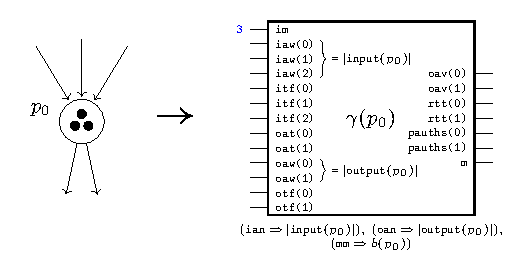
\includegraphics[keepaspectratio,width=.7\textwidth]{gen-pci-ex.eps}
    \caption{A graphical representation of the interface of the PDI
      $\gamma(p_0)$ (on the right) implementing place $p_0$ (on the
      left). The generic map associations appear underneath the PDI.}
    \label{fig:gen-pci-ex}
  \end{figure}
  
  \begin{enumerate}[resume]

  \item\label{it:exists-tdi} For all transition of the input SITPN model, there exists a
    corresponding TDI identified through $\gamma$ in the behavior of
    the output design:\\
    $\forall{}t\in{}T,\exists{}g_t,i_t,o_t$ s.t. $\tdiInBeh$.
    
  \item\label{it:tdi-gen-map} For all transition of the input SITPN model and its
    corresponding TDI, the generic map of the TDI holds the following
    associations:
    \begin{equation*}
      \begin{aligned}[t]
        \forall{}t&\in{}T,g_t,i_t,o_t, \\
                  & \tdiInBeh\Rightarrow \\
                  &
                    \begin{aligned}[t]
                      g_t=\{&(\mathtt{tt}\Rightarrow{}
                      \begin{cases}
                        \mathtt{not\_temp}~\mathrm{if}~t\notin{}\mathtt{dom}(I_s) \\
                        \mathtt{temp\_a\_a}~\mathrm{if}~I_s(t)=[a,a] \\
                        \mathtt{temp\_a\_b}~\mathrm{if}~I_s(t)=[a,b] \\
                        \mathtt{temp\_a\_inf}~\mathrm{if}~I_s(t)=[a,\infty] \\
                      \end{cases}),\\
                      & (\mathtt{mtc}\Rightarrow
                      \begin{cases}
                        1~\mathrm{if}~t\notin{}\mathtt{dom}(I_s) \\
                        b~\mathrm{if}~I_s(t)=[a,b] \\
                        a~\mathrm{if}~I_s(t)=[a,\infty] \\
                      \end{cases}), \\
                      & (\mathtt{ian}\Rightarrow
                        \begin{cases}
                          1~\mathrm{if}~\mathtt{input}(t)=\emptyset \\
                          \vert{}\mathtt{input}(t)\vert~\mathrm{otherwise} \\
                        \end{cases}), 
                      (\mathtt{cn}\Rightarrow
                      \begin{cases}
                        1~\mathrm{if}~\mathtt{conds}(t)=\emptyset \\
                        \vert{}\mathtt{conds}(t)\vert~\mathrm{otherwise} \\
                      \end{cases})\}. \\
                    \end{aligned} \\
      \end{aligned}
    \end{equation*}
    where
    \texttt{input}$(t)=\{p~\vert~pre(p,t)=\lfloor(\omega,a)\rfloor\}$,
    the set of input places of transition $t$, and
    \texttt{conds}$(t)=\{c~\vert~\mathbb{C}(t,c)=1\lor\mathbb{C}(t,c)=-1\}$,
    the set of conditions associated with transition $t$.
    
  \item\label{it:tdi-time-itval} For all transition of the input SITPN
    model and its corresponding TDI, the input port map of the TDI
    holds the following associations:
    \begin{equation*}
      \begin{aligned}[t]
        \forall{}t&\in{}T,g_t,i_t,o_t, \\
                  & \tdiInBeh\Rightarrow \\
                  &
                    \begin{aligned}[t]
                      \{&(\mathtt{A}\Rightarrow\begin{cases}
                                                0~\mathrm{if}~t\notin\mathtt{dom}(I_s) \\
                                                l(I_s(t))~\mathrm{otherwise} \\
                                              \end{cases}), \\
                      & (\mathtt{B}\Rightarrow\begin{cases}
                                              0~\mathrm{if}~t\notin\mathtt{dom}(I_s)\lor{}u(I_s(t))=\infty \\
                                              u(I_s(t))~\mathrm{otherwise} \\
                                            \end{cases})\}\subseteq{}i_t. \\
                    \end{aligned}
        \\
      \end{aligned}
    \end{equation*}

  \end{enumerate}

  \bigskip

  Similarly to the case of places, Points~\ref{it:exists-tdi} to
  \ref{it:tdi-time-itval} state the existence of a corresponding TDI
  for each transition of the input model, and specify how its generic
  map and its input port map must be built regarding the properties of
  the transition, namely: the shape of the time interval, the number
  of input arcs, the number of associated
  conditions. Figure~\ref{fig:gen-tdi-ex} illustrates how the
  properties of a transition are implemented in the interface of the
  corresponding TDI.

  \begin{figure}[h]
    \centering
    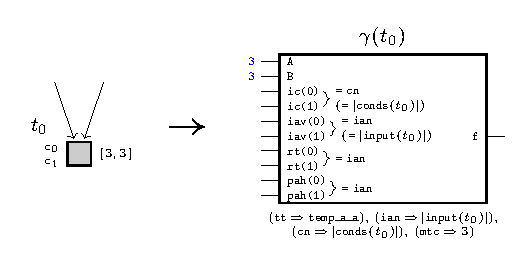
\includegraphics[keepaspectratio,width=.8\textwidth]{gen-tdi-ex.eps}
    \caption{A graphical representation of the interface of the TDI
      $\gamma(t_0)$ (on the right) implementing transition $t_0$ (on
      the left). The generic map associations appear underneath the
      TDI.}
    \label{fig:gen-tdi-ex}
  \end{figure}
  
  \begin{enumerate}[resume]        
  \item\label{it:post-arc} For all post arc of the input SITPN model,
    the TDI and PDI corresponding to the source transition and target
    place of the arc are connected as follows:
    \begin{equation*}
      \begin{aligned}[t]
        \forall{}t&\in{}T,p\in{}P,g_t,i_t,o_t,g_p,i_p,o_p,\omega\in\mathbb{N}^{*}, \\
                  & post(t,p)=\lfloor\omega\rfloor\Rightarrow \\
                  & \tdiInBeh\Rightarrow \\
                  & \pdiInBeh\Rightarrow\\
                  &
                    \begin{aligned}[t]
                      \exists{}i & \in[0,\vert\mathtt{input}(p)\vert-1]~s.t.~(\mathtt{iaw}(i)\Rightarrow\omega)\in{}i_p \\
                                 & \land\exists{}id_s~s.t.~(id_s,\mathtt{bool})\in{}d.sigs
                                   \land(\mathtt{fired}\Rightarrow{}id_s)\in{}o_t\land(\mathtt{itf}(i)\Rightarrow{}id_s)\in{}i_p. \\
                    \end{aligned}
        \\
      \end{aligned}
    \end{equation*}
  \end{enumerate}
  
  \bigskip

  In Point~\ref{it:post-arc}, $(id_s,\mathtt{bool})\in{}d.sigs$
  indicates the signal $id_s$ is declared as a Boolean internal signal
  in the output design. Figure~\ref{fig:gen-post-arc} illustrates the
  translation of a post arc of the input SITPN model as described in
  Point~\ref{it:post-arc}. The weight of the arc is passed to the PDI
  through the \texttt{iaw} (for \texttt{input\_arcs\_weights}) input
  port. In the behavior of the output design, all arc information is
  encoded through the input port interface of PDIs. All computations
  that necessitate the arc information, such as the marking update or
  the setting of time counter reset signals, are performed in the
  behavior of the place design. Therefore, only the PDIs need to hold
  the arc information.

  \begin{figure}[h]
    \centering
    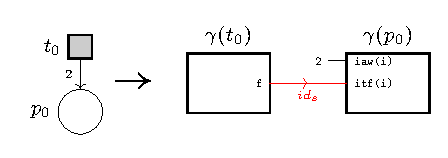
\includegraphics[keepaspectratio,width=.7\textwidth]{gen-post-arc.eps}
    \caption{The translation of a post arc, connecting a transition
      $t_0$ to a place $p_0$, into an interconnection between the
      interfaces of the corresponding TDI and PDI.}
    \label{fig:gen-post-arc}
  \end{figure}
  
  \begin{enumerate}[resume]
  \item\label{it:pre-arc} For all pre arc of the input SITPN model,
    the PDI and TDI corresponding to the source place and target
    transition of the arc are connected as follows:
    \begin{equation*}
      \begin{aligned}[t]
        \forall{}t&\in{}T,p\in{}P,g_t,i_t,o_t,g_p,i_p,o_p,\omega\in\mathbb{N}^{*},a\in\{\mathtt{basic},\mathtt{test},\mathtt{inhib}\}, \\
                  & pre(p,t)=\lfloor(\omega,a)\rfloor\Rightarrow \\
                  & \tdiInBeh\Rightarrow \\
                  & \pdiInBeh\Rightarrow\\
                  & \exists{}i\in[0,\vert\mathtt{output}(p)\vert-1]~s.t.~\{(\mathtt{oaw}(i)\Rightarrow\omega),(\mathtt{oat}(i)\Rightarrow{}a)\}\subseteq{}i_p \\
                  & \begin{aligned}[t]
                      \land\exists{}j &\in[0,\vert\mathtt{input}(t)\vert-1],id_{av},id_{rt},id_{frd},id_{pah}~s.t. \\
                                      & \{(id_{av},\mathtt{bool}),(id_{rt},\mathtt{bool}),(id_{frd},\mathtt{bool}),(id_{pah},\mathtt{bool})\}\subseteq{}d.sigs \\
                                      & \land(\mathtt{oav}(i)\Rightarrow{}id_{av})\in{}o_p\land(\mathtt{iav}(j)\Rightarrow{}id_{av})\in{}i_t \\
                                      & \land(\mathtt{rtt}(i)\Rightarrow{}id_{rt})\in{}o_p\land(\mathtt{rt}(j)\Rightarrow{}id_{rt})\in{}i_t \\
                                      & \land(\mathtt{otf}(i)\Rightarrow{}id_{frd})\in{}i_p\land(\mathtt{fired}\Rightarrow{}id_{frd})\in{}o_t \\
                                      & \land(\mathtt{pah}(i)\Rightarrow{}id_{frd})\in{}o_p \\
                                      & \land(a=\mathtt{test}\lor{}a=\mathtt{inhib}\lor{}\mathtt{confl}(p)=\emptyset\Rightarrow(\mathtt{pah}(j)\Rightarrow\mathtt{true})\in{}i_t) \\
                                      & \land(a=\mathtt{basic}\land{}\mathtt{confl}(p)\neq\emptyset~or~\mathtt{err}\Rightarrow(\mathtt{pah}(j)\Rightarrow{}id_{pah})\in{}i_t). \\
                    \end{aligned} \\
      \end{aligned}
    \end{equation*}
    where $\mathtt{confl}\in{}P\rightarrow{}2^T\cup\{\mathtt{err}\}$
    takes a place $p$ as input and yields either an error or an
    ordered set of transitions computed as follows:
    \begin{enumerate}
    \item If all conflicts between the output transitions of $p$ are
      solved by mutual exclusion, or if the set of conflicting
      transitions of $p$ is a singleton, then $\mathtt{confl}$ returns
      an empty set.
    \item Otherwise, the function tries to establish a total ordering
      over the set of conflicting transitions of $p$ w.r.t the firing
      priority relation:
      \begin{itemize}
      \item If no such ordering can be established (in that case, the
        firing priority relation is ill-formed, and the input SITPN is
        not well-defined), $\mathtt{confl}$ returns the \texttt{err}
        value.
      \item Otherwise, the function returns the set in a decreasing
        priority order.
      \end{itemize}
    \end{enumerate}
    
  \end{enumerate}

  \bigskip
  
  Figure~\ref{fig:gen-pre-arc} illustrates the translation of a pre
  arc of the input SITPN model as described in Point~\ref{it:pre-arc}.
  As for the post arcs, the arc information is passed through the
  input port map of the PDI. As there are three possible types of pre
  arc, the \texttt{oat} (for \texttt{output\_arcs\_types}) input port
  receives the arc type information.  In Figure~\ref{fig:gen-pre-arc},
  we assume that there remain some conflicts not solved by mutual
  exclusion in the set of output transitions of place
  $p_0$. Otherwise, according to Point~\ref{it:pre-arc}, the
  interconnection between $\mathtt{pah(i)}$ and $\mathtt{pah(j)}$
  would not be effective.
  
  \begin{figure}[h]
    \centering
    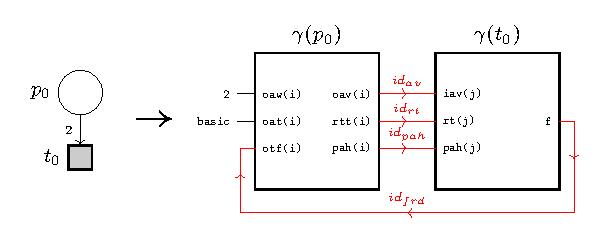
\includegraphics[keepaspectratio,width=.8\textwidth]{gen-pre-arc.eps}
    \caption{The translation of a pre arc, connecting a place $p_0$ to
      a transition $t_0$, into signal interconnections between the
      interfaces of the corresponding PDI and TDI. }
    \label{fig:gen-pre-arc}
  \end{figure}

  \begin{enumerate}[resume]
  \item\label{it:port-indices-ordering} For all place of the input
    SITPN model for which conflicts in its output transitions are not
    solved by mutual exclusion, the port indices of the corresponding
    PDI reflect the priority order established between the conflicting
    output transitions:
    \begin{equation*}
      \begin{aligned}[t]
        \forall{}p&\in{}P,t,t'\in{}\mathtt{confl}(p),g_p,i_p,o_p,g_t,i_t,o_t,g_{t'},i_{t'},o_{t'}, \\
                  & t\succ{}t'\Rightarrow\\
                  & \pdiInBeh\Rightarrow \\
                  & \tdiInBehP{t}\Rightarrow \\
                  & \tdiInBehP{t'}\Rightarrow \\
                  &
                    \begin{aligned}[t]
                      (\forall{}i,j&\in\mathbb{N},id_{frd},id_{frd'},id_{s},id_{s'},name_t,name_{t'},id_{out}, \\
                                   & (\mathtt{fired}\Rightarrow{}id_{frd})\in{}o_t\Rightarrow \\
                                   & (\mathtt{fired}\Rightarrow{}id_{frd'})\in{}o_{t'}\Rightarrow \\
                                   & \{(\mathtt{otf}(i)\Rightarrow{}id_{frd}),(\mathtt{otf}(j)\Rightarrow{}id_{frd'})\}\subseteq{}i_p\Rightarrow \\
                                   & (name_t\Rightarrow{}id_{s})\in{}i_t\Rightarrow \\
                                   & (name_{t'}\Rightarrow{}id_{s'})\in{}i_{t'}\Rightarrow \\
                                   & \{(id_{out}(i)\Rightarrow{}id_s),(id_{out}(j)\Rightarrow{}id_{s'})\}\subseteq{}o_p\Rightarrow \\
                                   & i<j) \\
                    \end{aligned} \\
      \end{aligned}
    \end{equation*}
  \end{enumerate}

  \bigskip

  As specified in Point~\ref{it:port-indices-ordering}, the port
  indices in the interface of a PDI must reflect the priority order
  established between its \textit{conflicting} TDIs. Of course, this
  is only mandatory for the ports connecting the PDI to its
  conflicting TDIs. Otherwise, the index order does not matter, for
  instance while reifying a post arc connection.
  Figure~\ref{fig:gen-prio-order} illustrates the ordering of the port
  indices in the interface of a PDI as described in
  Point~\ref{it:port-indices-ordering}.

  \begin{figure}[h]
    \centering
    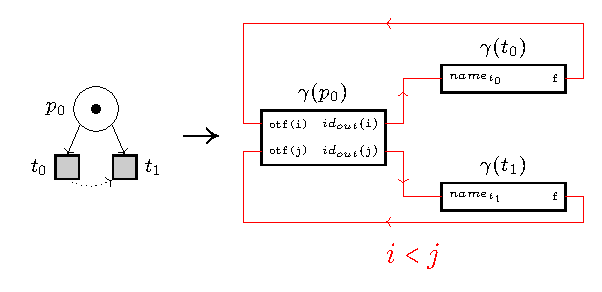
\includegraphics[keepaspectratio,width=.8\textwidth]{gen-prio-order.eps}
    \caption{Translation of the priority relation in terms of port
      index ordering. On the right, $name_{t_0}$ (resp. $name_{t_1}$)
      refers to any input port of TDI $\gamma(t_0)$
      (resp. $\gamma(t_1)$), and $id_{out}$ refers to any composite
      output port of PDI $\gamma(p_0)$. On the left, the dotted arc
      going from transition $t_0$ to $t_1$ indicates the $t_0$ has a
      higher firing priority than $t_1$. }
    \label{fig:gen-prio-order}
  \end{figure}

  \begin{enumerate}[resume]
  \item\label{it:actions} There exists an \texttt{actions} process
    that assigns a value to the output ports (referred to as
    \textit{action} ports) representing the activation status of the
    actions of the input SITPN model:
    
    $\exists{}ss_{ra},ss_{a}~s.t.~\mathtt{ps}(\mathtt{actions},\emptyset,\mathtt{rst}\{ss_{ra}\}\mathtt{else}\{\mathtt{falling}\{ss_a\}\})\in{}d.beh$
    and
    \begin{enumerate}
    \item The length of the $ss_{ra}$ and $ss_{a}$ sequences is equal
      to the number of actions of the input SITPN model:\\
      $\vert{}ss_{ra}\vert_{;}=\vert{}ss_a\vert_{;}=\vert\mathcal{A}\vert$
      where $\vert{}ss\vert{}_{;}=
      \begin{cases}
        \vert{}ss_1\vert_{;}+\vert{}ss_2\vert_{;}~\mathrm{if}~ss=ss_1;ss_2 \\
        1~\mathrm{otherwise}
      \end{cases}
      $
      
    \item During the initialization, all action ports are assigned to
      \texttt{false} by the \texttt{actions} process:
      $\forall{}a\in\mathcal{A},~\gamma(a)\Leftarrow\mathtt{false}\in{}ss_{ra}$
      
    \item An action port corresponding to an unassociated action is
      assigned to \texttt{false} during the falling edge
      phase:\\
      $\forall{}a\in\mathcal{A}~s.t.~\mathtt{pls}(a)=\emptyset,\gamma(a)\Leftarrow\mathtt{false}\in{}ss_{a}$
      where
      \texttt{pls}$(a)=\{p~\vert~\mathbb{A}(p,a)=\mathtt{true}\}$, the
      set of places associated with action $a$.
      
    \item Otherwise, the value of the action port is the result of the
      Boolean sum between the \texttt{marked} output port of all PDIs
      representing the places associated with the corresponding
      action:
      \begin{equation*}
        \begin{aligned}[t]
          \forall{}a&\in\mathcal{A},~\mathtt{pls}(a)\neq\emptyset\Rightarrow \\
                    &  \begin{aligned}[t]
                         \exists{}e_{or}& ~s.t.~\gamma(a)\Leftarrow{}e_{or}\in{}ss_a\land\mathtt{is\_bsum}(e_{or},\vert{}\mathtt{pls}(a)\vert) \\
                                        &
                                          \begin{aligned}
                                            \land\forall{}p& \in\mathtt{pls}(a),g_p,i_p,o_p, \\
                                                           & \pdiInBeh\Rightarrow \\
                                                           &
                                                             \begin{aligned}
                                                               \exists{}id_m& ~s.t.~(id_m,\mathtt{bool})\in{}d.sigs \\
                                                                            &\land{}id_m\in{}e_{or} \\
                                                                            & \land(\mathtt{marked}\Rightarrow{}id_m)\in{}o_p \\
                                                             \end{aligned} \\
                                          \end{aligned} \\
                       \end{aligned} \\
        \end{aligned}
      \end{equation*}
      where $\mathtt{is\_bsum}$ is defined as follows:

      \vspace{10pt}
      
      \begin{tabular}{l}
        {\begin{prooftree}
            \hypo{e\in{}\{id,b\}}
            \infer1{\mathtt{is\_bsum}(e,1)}
          \end{prooftree}} \\
      \end{tabular}
      \begin{tabular}{l}
        {\begin{prooftree}
            \hypo{\mathtt{is\_bsum}(e_1,n)}
            \hypo{\mathtt{is\_bsum}(e_2,m)}
            \infer2
            {\mathtt{is\_bsum}(\mathtt{or}(e_1,e_2),n+m)}
          \end{prooftree}} \\
      \end{tabular}
    \end{enumerate}
  \end{enumerate}

  \bigskip

  In Point~\ref{it:actions}, the $\mathtt{is\_bsum}$ relation states
  that a given expression is a Boolean sum (i.e. a composition of
  \texttt{or} expressions) of Boolean terminals or identifiers and
  that this expression has a given size. Through the \texttt{is\_bsum}
  relation, we want specify that all the internal signals connected to
  the \texttt{marked} ports of the associated PDIs are represented in
  the $e_{or}$ expression.  Figure~\ref{fig:gen-actions} describes the
  content of the \texttt{actions} process, obtained through the
  transformation of a given input SITPN model, as specified in
  Point~\ref{it:actions}. The specification of the \texttt{functions}
  process is very close to the definition of the \texttt{actions}
  process. The reader can find it in \cite{Iampietro2022hfspec}.
  
  \begin{figure}[!ht]
    \centering
    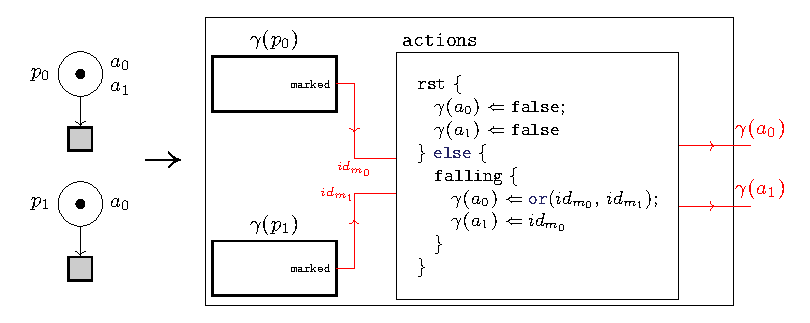
\includegraphics[keepaspectratio,width=\textwidth]{gen-actions.eps}
    \caption{The content of the \texttt{actions} process (on the
      right) based on the place-action associations of the input SITPN
      model (on the left). }
    \label{fig:gen-actions}
  \end{figure}

  \bigskip
  
  \begin{enumerate}[resume]
  \item\label{it:cond-ports} For all association between a transition and a condition, the
    input port (referred to as a \textit{condition} port) reflecting
    the Boolean value of the given condition is connected as follows
    to the input port map of the TDI corresponding to the associated
    transition:
    \begin{equation*}
      \begin{aligned}[t]
        \forall{}t&\in{}T,g_t,i_t,o_t,c\in\mathcal{C}, \\
                  & \tdiInBeh\Rightarrow \\
                  & (\mathbb{C}(t,c)=1\Rightarrow\exists{}i\in[0,\vert\mathtt{conds}(t)\vert-1]~s.t.~(\mathtt{ic}(i)\Rightarrow{}\gamma(c))\in{}i_t) \\
                  & (\mathbb{C}(t,c)=-1\Rightarrow\exists{}i\in[0,\vert\mathtt{conds}(t)\vert-1]~s.t.~(\mathtt{ic}(i)\Rightarrow{}\mathtt{not}(\gamma(c)))\in{}i_t). \\
      \end{aligned}
    \end{equation*}

  \end{enumerate}

  Figure~\ref{fig:gen-conds} illustrates the connection between a
  condition port and its associated TDIs as specified in
  Point~\ref{it:cond-ports}. Condition ports are connected to the
  \texttt{ic} (for \texttt{input\_conditions}) input port of their
  associated TDIs.
  
  \begin{figure}[h]
    \centering
    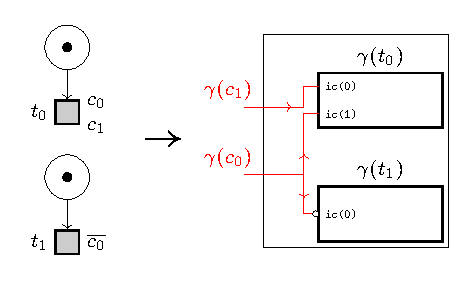
\includegraphics[keepaspectratio,width=.65\textwidth]{gen-conds.eps}
    \caption{Translation of the condition-transition associations (on
      the left) into interconnections between condition ports and
      TDIs' interfaces (on the right). }
    \label{fig:gen-conds}
  \end{figure}

  To conclude the definition of the $HM2T_{\mathtt{spec}}$ relation,
  we have $HM2T_{\mathtt{spec}}(sitpn,b,\mathtt{err})$ if $sitpn$ is
  not a well-defined SITPN model w.r.t. Definition~\ref{def:wd-sitpn}.
\end{definition}

%%% Local Variables:
%%% mode: latex
%%% TeX-master: "main"
%%% End:

% \section{Proof of semantic preservation}
\label{sec:proof}

The semantic preservation property of the HM2T is expressed by a
\textit{forward simulation} theorem, which general form is as follows
(according to \cite{Leroy2009}):
\begin{equation*}
  \forall{}S,C,B,\mathtt{transf}(S)=C\land{}S\Downarrow{}B\Rightarrow{}\exists{}B'~s.t.~C\Downarrow{}B'\land{}B\sim{}B'.
\end{equation*}

Considering the above theorem in a more general framework than the one
of compilers from programming languages (which is the framework of
\cite{Leroy2009}), $S$ corresponds to an instance of a source
formalism, and $C$ is the result of the transformation of $S$ by the
transformation function $\mathtt{transf}$; $C$ is an instance of a
target formalism. $B$ and $B'$ are behaviors, and the binary relation
$\Downarrow$ states that a given instance of a formalism has a given
behavior. $B\sim{}B'$ states that the behavior $B$ is similar to the
behavior $B'$ considering a contextual definition of the similarity
relation. The forward simulation theorem must be read as follows: for
all instance $S$ of a source formalism transformed into $C$ by
function $\mathtt{transf}$, if $S$ has a behavior $B$, then $C$ has a
behavior $B'$ that is similar to $B$. In our case, we have proved a
slightly different theorem, which has the following form:
\begin{equation*}
  \forall{}S,C,B,B',~\mathtt{transf}(S)=C\land{}S\Downarrow{}B\land{}C\Downarrow{}B'\Rightarrow{}B\sim{}B'.
\end{equation*}
In the above form, we consider that the target $C$ has the behavior
$B'$, and we no more have to prove the existence of such a behavior.
This version of the theorem focuses on the behavior similarity. Thus,
we refer to it has a behavior (or trace) similarity theorem. In our
work perspectives, we contrive to prove the first form of the theorem,
but in this article we will present the proof of the second form.

In our specific transformation case, $S$ is a SITPN model and $C$ is a
\hvhdl{} design. The behavior of a SITPN model and a \hvhdl{} design
corresponds to the execution trace computed through a certain number
of clock cycles w.r.t. semantics rules that have been presented in
Sections~\ref{subsec:hpn-particularities} and
\ref{subsec:sim-semantics}. Thus, the property of semantic
preservation for the HM2T is about comparing the execution traces of
the input SITPN model and the output \hvhdl{} design. Specifically, we
want to show that, no matter how much clock cycles are performed, the
execution traces are always
\textit{similar}. Figure~\ref{fig:trace-comparison} illustrates the
comparison of the execution traces of a SITPN model input of the HM2T
and its corresponding output design.
\begin{figure}[!ht]
  \centering
  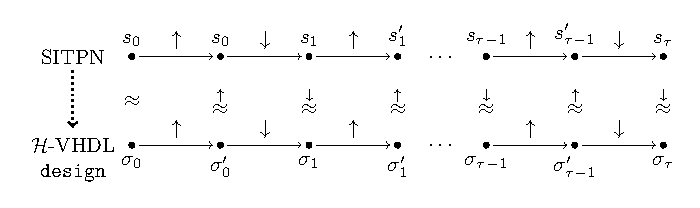
\includegraphics[keepaspectratio,width=\textwidth]{trace-comparison-full.eps}
  \caption{Comparison between the execution trace of a SITPN model (on
    the upper part) and the execution trace of the \hvhdl{} design
    resulting from the HM2T (on the lower part). The $\uparrow$
    (resp. $\downarrow$) symbol represents a rising (resp. falling)
    edge step happening in the course of a clock cycle. The $\approx$
    symbol represents the similarity relation between the upper SITPN
    state and the lower \hvhdl{} design state.}
  \label{fig:trace-comparison}
\end{figure}

In Figure~\ref{fig:trace-comparison}, $\tau$ indicates an arbitrary
number of clock cycles. To perform the proof of semantic preservation,
we must prove that every pair of states considered at the same time
point are similar w.r.t. to our own similarity relation.  Let us
introduce our general similarity criterions between a SITPN state and
a \hvhdl{} state through the relation presented in
Definition~\ref{def:state-sim}.

\begin{definition}[State similarity relation]
  \label{def:state-sim}
  For a given $sitpn\in{}SITPN$, a \hvhdl{} design $d\in{}design$, and
  a binder $\gamma\in{}WM(sitpn,d)$, an SITPN state $s\in{}S(sitpn)$
  and a design state $\sigma\in\Sigma$ are similar, written
  $\gamma\vdash{}s\approx\sigma$ if
  \begin{enumerate}
  \item\label{item:sim-mark} $\forall{}p\in{}P,$
    $~s.M(p)=\sigma(\gamma(p))($\texttt{s\_marking}$)$.
  \item\label{item:sim-tc}
    $\forall{}t\in{}T_i,$\\
    $\big(u(I_s(t))=\infty\land{}s.I(t)\le{}l(I_s(t))\Rightarrow{}s.I(t)=\sigma(\gamma(t))($\texttt{s\_time\_counter}$)\big)$\\
    $\land\big(u(I_s(t))=\infty\land{}s.I(t)>{}l(I_s(t))\Rightarrow{}\sigma(\gamma(t))($\texttt{s\_time\_counter}$)=l(I_s(t))\big)$\\
    $\land\big(u(I_s(t))\neq\infty\land{}s.I(t)>{}u(I_s(t))\Rightarrow{}\sigma(\gamma(t))($\texttt{s\_time\_counter}$)=u(I_s(t))\big)$\\
    $\land\big(u(I_s(t))\neq\infty\land{}s.I(t)\le{}u(I_s(t))\Rightarrow{}s.I(t)=\sigma(\gamma(t))($\texttt{s\_time\_counter}$)\big)$.
  \item\label{item:sim-reset} $\forall{}t\in{}T_i,$
    $s.reset_t(t)=\sigma(\gamma(t))($\texttt{s\_reinit\_time\_counter}$)$.
  \item\label{item:sim-cond}
    $\forall{}c\in\mathcal{C},~s.cond(c)=\sigma(\gamma(c))$.
  \item\label{item:sim-act}
    $\forall{}a\in\mathcal{A},~s.ex(a)=\sigma(\gamma(a))$.
  \item\label{item:sim-fun}
    $\forall{}f\in\mathcal{F},~s.ex(f)=\sigma(\gamma(f))$.
  \end{enumerate}
\end{definition}

In Definition~\ref{def:state-sim}, the binder structure $\gamma$ that
is generated by the HM2T relates the elements of the SITPN model to
the elements of the \hvhdl{} design, and thus enables the comparison
between the SITPN state and the design state. In
Definition~\ref{def:state-sim}, Point~\ref{item:sim-mark} relates the
marking value of a place $p$ at state $s$ to the value of the
\texttt{s\_marking} signal, which is an internal signal of the PDI
identified by $\gamma(p)$. Here, the expression $\sigma(\gamma(p))$
returns the internal state of the PDI $\gamma(p)$ by looking up the
component store of state $\sigma$. Point~\ref{item:sim-tc} (resp.
Point~\ref{item:sim-reset} similarly relate the value of time counters
(resp. reset orders) of transitions to the value of the
$\texttt{s\_time\_counter}$ signal
(resp. $\texttt{s\_reinit\_time\_counter}$) in the internal state of
the corresponding TDIs. In Point~\ref{item:sim-cond}
(resp. \ref{item:sim-act} and \ref{item:sim-fun}), the Boolean value
of conditions (resp. actions and functions) are compared to the value
of the input (resp. output) ports of the output design, also based on
the $\gamma$ binder.  As one can observe in Point~\ref{item:sim-tc},
due to the specific implementation of time intervals with an infinite
upper bound in \hvhdl{}, the relation between the value of a time
counter and the value of the $\texttt{s\_time\_counter}$ signal can
not be restricted to a simple equality.

As shown in Figure~\ref{fig:trace-comparison}, we make a distinction
between the state similarity after a rising edge phase and after a
falling edge phase. The definitions of the post rising edge similarity
relation, written $\stackrel{\uparrow}{\approx}$, and the post falling
edge similarity relation, written $\stackrel{\uparrow}{\approx}$, are
restrictions of the general definition. After a rising edge phase, the
equality between the value of conditions and the value of condition
ports (i.e. Point~\ref{item:sim-cond} of
Definition~\ref{def:state-sim}) does not hold, and after a falling
edge phase, the equality between the value of time counter reset
orders and the value of the \texttt{s\_reinit\_time\_counter} signals
(i.e. Point~\ref{item:sim-reset} of Definition~\ref{def:state-sim})
does not hold. However, these divergences do not impact the
computation logic of the overall so that to create further behavioral
divergences between the input SITPN model and the output \hvhdl{}
design.

Definition~\ref{def:exec-trace-sim} introduces the relation that
states that a SITPN model's execution trace is similar to a \hvhdl{}
design's execution trace.

\begin{definition}[Execution trace similarity]
  \label{def:exec-trace-sim}
  For a given $sitpn\in{}SITPN$, a \hvhdl{} design $d\in{}design$, and
  a binder $\gamma\in{}WM(sitpn,d)$, the execution trace
  $\theta_s\in{}\mathtt{list}(S(sitpn))$ and the simulation trace
  $\theta_\sigma\in\mathtt{list}(\Sigma)$ are similar, written
  $\gamma\vdash{}\theta_s\stackrel{clk}{\sim}\theta_\sigma$ where
  $clk\in\{\uparrow,\downarrow\}$, according to the following rules:\\

  \begin{tabular}{@{}l}
    {\begin{prooftree}[template={\inserttext}]        
        \infer0[$clk\in{}\{\uparrow,\downarrow\}$]{$\gamma\vdash{}[~]\stackrel{clk}{\sim}{}[~]$}
      \end{prooftree}} 
  \end{tabular}
  \begin{tabular}{@{}l}
    {\begin{prooftree}[template={\inserttext}]

        \hypo{$\gamma\vdash{}s\stackrel{\uparrow}{\sim}\sigma$}
        \hypo{$\gamma\vdash{}\theta_s\stackrel{\downarrow}{\sim}{}\theta_\sigma$}
        \infer2{$\gamma\vdash{}(s :: \theta_s)\stackrel{\uparrow}{\sim}{}(\sigma :: \theta_\sigma)$}
      \end{prooftree}} 
  \end{tabular}
  \begin{tabular}{@{}l}
    {\begin{prooftree}[template={\inserttext}]

        \hypo{$\gamma\vdash{}s\stackrel{\downarrow}{\sim}\sigma$}
        \hypo{$\gamma\vdash{}\theta_s\stackrel{\uparrow}{\sim}{}\theta_\sigma$}
        \infer2{$\gamma\vdash{}(s :: \theta_s)\stackrel{\downarrow}{\sim}{}(\sigma :: \theta_\sigma)$}
      \end{prooftree}} 
  \end{tabular}
\end{definition}

In Definition~\ref{def:exec-trace-sim}, the clock event symbol on top
of the $\sim$ sign indicates the kind of clock event that led to the
production of the states at the head of the traces. The execution
trace similarity relation expects that the states composing the traces
have been alternatively produced by a rising edge step followed by a
falling edge step. By construction, the traces must have the same
length to respect the execution trace similarity relation.

To handle the case of an execution/simulation trace beginning by an
initial state, that is, a state neither reached after a rising nor
after a falling edge, we give a slightly different definition of the
execution trace similarity relation in
Definition~\ref{def:full-exec-trace-sim}.

\begin{definition}[Full execution trace similarity]
  \label{def:full-exec-trace-sim} For a given $sitpn\in{}SITPN$, a
  \hvhdl{} design $d\in{}design$, and a binder
  $\gamma\in{}WM(sitpn,d)$, the execution trace
  $\theta_s\in{}\mathtt{list}(S(sitpn))$ and the simulation trace
  $\theta_\sigma\in\mathtt{list}(\Sigma)$ are fully similar, written
  $\gamma\vdash{}\theta_s\sim\theta_\sigma$, according to the
  following rules:\\

  \begin{tabular}{l}
    {\begin{prooftree}[template={\inserttext}]
        \infer0{$\gamma\vdash{}[~]\sim{}[~]$}
      \end{prooftree}}
  \end{tabular}
  \begin{tabular}{l}
    {\begin{prooftree}[template={\inserttext}]

        \hypo{$\gamma\vdash{}s\sim\sigma$}
        \hypo{$\gamma\vdash{}\theta_s\stackrel{\uparrow}{\sim}{}\theta_\sigma$}
        \infer2{$\gamma\vdash{}(s :: \theta_s)\sim{}(\sigma ::
          \theta_\sigma)$}
      \end{prooftree}}
  \end{tabular}
\end{definition}

The full execution trace similarity relation indicates that the head
states of traces must verify the general state similarity relation
(cf. Figure~\ref{fig:trace-comparison}), and that the tail of the
traces must respect the execution state similarity relation starting
with a rising edge step.

Now, let us introduce the necessary lemmas to prove the semantic
preservation theorem. In Definition~\ref{def:hm2t-hyps}, we present
the hypotheses expressing the fact that we are proving the semantic
preservation property for the HM2T. These hypotheses will always
appear in the lemmas and theorems presented afterwards.

\begin{definition}[HM2T hypotheses]
  \label{def:hm2t-hyps}
  For all well-defined $sitpn\in{}SITPN$, bounding function
  $b\in{}P\rightarrow\mathbb{N}$, \hvhdl{} design $d\in{}design$,
  binder $\gamma\in{}WM(sitpn,d)$, elaborated design
  $\Delta\in{}ElDesign$, default state $\sigma_e\in\Sigma$, simulation
  environment $E_p\in\mathbb{N}\rightarrow{}(id\nrightarrow{}v)$, and
  execution environment
  $E_c\in\mathbb{N}\rightarrow(\mathcal{C}\rightarrow\mathbb{B})$,
  assume that:
  \begin{enumerate}
  \item\label{it:HM2T-some} Taking the SITPN model $sitpn$ and the
    bounding function $b$ as inputs, the HM2T returns an output design
    $d$ and a binder $\gamma$, written
    $\mathtt{sitpn2hvhdl}(sitpn, b)=\lfloor(d,\gamma)\rfloor$ where
    $\mathtt{sitpn2hvhdl}\in{}SITPN\rightarrow(P\rightarrow\mathbb{N})\nrightarrow(design\times{}WM(sitpn,d))$.
  \item\label{it:sitpn-is-bounded} $sitpn$ is bounded through $b$,
    written $\lceil{}sitpn\rceil^b$.
  \item In the context of the \hilecop{} design store
    $\mathcal{D}_\mathcal{H}$ and with an empty generic constant
    dimensioning function ($\emptyset$), $d$ is elaborated into
    $\Delta$ with a default state $\sigma_e$, written
    $\mathcal{D}_\mathcal{H},\emptyset\vdash{}d\xrightarrow{elab}\Delta,\sigma_e$.
  \item\label{it:env-are-sim} Simulation and execution environments
    are similar, written $\gamma\vdash{}E_p\stackrel{env}{=}E_c$.
  \end{enumerate}
  
\end{definition}

In Point~\ref{it:HM2T-some} of Definition~\ref{def:hm2t-hyps}, the
$\mathtt{sitpn2hvhdl}$ function implements the HM2T, that is a
function proved sound and complete w.r.t. to the specification
presented in Section~\ref{sec:m2t}. Point~\ref{it:sitpn-is-bounded}
expresses the boundedness property of the input SITPN
model. Point~\ref{it:env-are-sim} states that, at each time point, the
execution and simulation environments yield the same Boolean value for
all couple condition-condition port linked through $\gamma$.

\def\hm2thyps{well-defined $sitpn\in{}SITPN$,
  $b\in{}P\rightarrow\mathbb{N}$, $d\in{}design$,
  $\gamma\in{}WM(sitpn,d)$, $\Delta\in{}ElDesign,\sigma_{e}\in\Sigma$,
  $E_p\in\mathbb{N}\rightarrow{}(id\nrightarrow{}v)$, and
  $E_c\in\mathbb{N}\rightarrow(\mathcal{C}\rightarrow\mathbb{B})$ that
  verify the hypotheses of Definition~\ref{def:hm2t-hyps}}

As illustrated in Figure~\ref{fig:trace-comparison}, to prove that the
execution traces are similar, we must first prove that the two initial
states are similar. This is expressed by
Lemma~\ref{lem:sim-init-states}.
\begin{lemma}[Similar initial states]
  \label{lem:sim-init-states}
  For all \hm2thyps{}, and for all $\sigma_0,\sigma_i\in{}\Sigma$ such that:
  \begin{itemize}
  \item $\sigma_0$ is the initial state of design $d$:\\
    $\mathcal{D},\Delta,\sigma_e\vdash{}d.beh\xrightarrow{cs_i}{}\sigma_i$ and
    $\mathcal{D},\Delta,\sigma_i\vdash{}d.beh\xrightarrow{\rightsquigarrow}{}\sigma_0$
  \end{itemize}
  then $\gamma\vdash{}s_0\approx\sigma_0$.
\end{lemma}

Starting from two similar initial states, then we must prove that each
phase, or step, of a clock cycle produces still similar states.  This
is expressed by \textit{lock-step simulation} lemmas \cite{Leroy2009},
which are of the following form in their \textit{non-existantial}
version:
\begin{equation*}
  \forall{}S_1,S'_1,S_2,S'_2,~S1\rightarrow{}S'_1\land{}S_2\rightarrow{}S'_2\land{}S_1\approx{}S_2\Rightarrow{}S'_1\approx{}S'_2.
\end{equation*}
Here, $S_1$ and $S'_1$ are two states of the source formalism, $S_2$
and $S'_2$ are two states of the target formalism.
$S_1\rightarrow{}S'_1$ (resp. $S_2\rightarrow{}S'_2$) states that an
execution step leads from $S_1$ to $S'_1$ (resp. from $S_2$ to $S'_2$)
w.r.t. a contextual definition of the execution
step. $S_1\approx{}S_2$ indicates that $S_1$ and $S_2$ are similar,
also w.r.t. a contextual definition of state similarity. The above
theorem must be read as follows: given two similar states $S_1$ and
$S_2$, if one execution step leads from $S_1$ to $S'_1$ and from $S_2$
to $S'_2$, then $S'_1$ and $S'_2$ are similar. \\

To establish the semantic preservation property, the first lock-step
simulation lemma that we had to prove pertains to the first rising
edge step. As defined in the SITPN semantics, the first rising edge
step is idle, i.e. a SITPN model is still in its initial state after
this step. Thus, we must prove that the state of the output design
reached after the first rising edge is similar to the SITPN model's
initial state. This is expressed by Lemma~\ref{lem:fst-re-lock-step}.

\begin{lemma}[First rising edge lock-step simulation]
  \label{lem:fst-re-lock-step}
  For all \hm2thyps{}, and for all clock count $\tau\in\mathbb{N}$,
  $\sigma_0,\sigma_i,\sigma_{\uparrow},\sigma'_0\in{}\Sigma$ such that:
  \begin{itemize}
  \item $\sigma_0$ is the initial state of design $d$:\\
    $\mathcal{D},\Delta,\sigma_e\vdash{}d.beh\xrightarrow{cs_i}{}\sigma_i$ and
    $\mathcal{D},\Delta,\sigma_i\vdash{}d.beh\xrightarrow{\rightsquigarrow}{}\sigma_0$
    
  \item a rising edge step leads from $\sigma_0$ to $\sigma'_0$:\\
    $\mathcal{D}_\mathcal{H},\Delta,\mathtt{inj}(\sigma_0,E_p,\tau)\vdash{}d.beh\xrightarrow{cs_{\uparrow}}\sigma_{\uparrow}$
    and
    $\mathcal{D}_\mathcal{H},\Delta,\sigma_{\uparrow}\vdash{}d.beh\xrightarrow{\rightsquigarrow}\sigma'_0$
  \end{itemize}
  then $\gamma\vdash{}s_0\stackrel{\uparrow}{\approx}\sigma'_0$.
\end{lemma}
In Lemma~\ref{lem:fst-re-lock-step}, $s_0$ is the initial state of the
SITPN model as introduced in
Definition~\ref{def:sitpn-init-state}.  Note that a rising edge step on the \hvhdl{} side refers to the conjunction of the three following phases: the injection of fresh values in primary input ports (through the use of the \texttt{inj} function), the execution of rising blocks, and the stabilization of combinational parts. \\

Then, we must prove that any rising edge or falling edge step verifies
the lock-step simulation property. This is expressed by
Lemmas~\ref{lem:re-lock-step} and \ref{lem:fe-lock-step}. 

\begin{lemma}[Rising edge lock-step simulation]
  \label{lem:re-lock-step}
  For all \hm2thyps{}, and for all $\tau\in\mathbb{N}$,
  $s,s'\in{}S(sitpn)$, $\sigma,\sigma_\uparrow,\sigma'\in\Sigma$, such
  that
  \begin{itemize}
  \item $s$ and $\sigma$ are similar states as intended after a
    falling edge step:
    $\gamma\vdash{}s\stackrel{\downarrow}{\approx}\sigma$
  \item a rising edge step leads from $s$ to $s'$:
    $E_c,\tau\vdash{}s\xrightarrow{\uparrow}s'$
  \item a rising edge step leads from $\sigma$ to $\sigma'$:\\
    $\mathcal{D}_\mathcal{H},\Delta,\mathtt{inj}(\sigma,E_p,\tau)\vdash{}d.beh\xrightarrow{cs_{\uparrow}}\sigma_{\uparrow}$
    and
    $\mathcal{D}_\mathcal{H},\Delta,\sigma_{\uparrow}\vdash{}d.beh\xrightarrow{\rightsquigarrow}\sigma'$
  \end{itemize}
  then $\gamma\vdash{}s'\stackrel{\uparrow}{\approx}{}\sigma'$.
  
\end{lemma}

\begin{lemma}[Falling edge lock-step simulation]
  \label{lem:fe-lock-step}
  For all \hm2thyps{}, and for all $\tau\in\mathbb{N}$,
  $s,s'\in{}S(sitpn)$, $\sigma,\sigma_\downarrow,\sigma'\in\Sigma$,
  such that
  \begin{itemize}
  \item $s$ and $\sigma$ are similar states as intended after a rising
    edge step: $\gamma\vdash{}s\stackrel{\downarrow}{\approx}\sigma$
  \item a falling edge step leads from $s$ to $s'$:
    $E_c,\tau\vdash{}s\xrightarrow{\downarrow}s'$
  \item a falling edge step leads from $\sigma$ to $\sigma'$:\\
    $\mathcal{D}_\mathcal{H},\Delta,\sigma\vdash{}d.beh\xrightarrow{cs_{\downarrow}}\sigma_{\downarrow}$
    and
    $\mathcal{D}_\mathcal{H},\Delta,\sigma_{\downarrow}\vdash{}d.beh\xrightarrow{\rightsquigarrow}\sigma'$
  \end{itemize}
  then $\gamma\vdash{}s'\stackrel{\downarrow}{\approx}{}\sigma'$.
\end{lemma}

As expressed in Lemma~\ref{lem:fe-lock-step}, a falling edge step on
the \hvhdl{} side refers to the execution of falling blocks followed
by the stabilization of combinational parts.\\

Under the assumptions of Lemma~\ref{lem:sim-init-states},
\ref{lem:fst-re-lock-step}, \ref{lem:re-lock-step} and
\ref{lem:fe-lock-step}, we can now prove the following trace
similarity theorem expressing that the HM2T is semantic preserving.

\begin{theorem}[Full trace similarity]
  \label{thm:full-trace-sim}
  For all well-defined $sitpn\in{}SITPN$, bounding function
  $b\in{}P\rightarrow\mathbb{N}$, \hvhdl{} design $d\in{}design$,
  binder $\gamma\in{}WM(sitpn,d)$, default state $\sigma_e\in\Sigma$,
  simulation environment
  $E_p\in\mathbb{N}\rightarrow{}(id\nrightarrow{}v)$, execution
  environment
  $E_c\in\mathbb{N}\rightarrow(\mathcal{C}\rightarrow\mathbb{B})$,
  $\tau\in\mathbb{N}$, SITPN model trace
  $\theta_s\in\mathtt{list}(S(sitpn))$, and \hvhdl{} design trace
  $\theta_\sigma\in\mathtt{list}(\Sigma)$ such that:
  \begin{enumerate}
  \item $\mathtt{sitpn2hvhdl}(sitpn, b)=\lfloor(d,\gamma)\rfloor$
  \item $\lceil{}sitpn\rceil^b$
  \item $\gamma\vdash{}E_p\stackrel{env}{=}E_c$
  \item $E_c,\tau\vdash{}sitpn\xrightarrow{full}\theta_s$
  \item
    $\mathcal{D}_\mathcal{H},\emptyset,E_p,\tau\vdash{}d\xrightarrow{full}\theta_\sigma$
  \end{enumerate}
  then $\gamma\vdash\theta_s\sim\theta_\sigma$.
\end{theorem}

\begin{pf}[Proof of Theorem~\ref{thm:full-trace-sim}.]
  
  Proceeding by case analysis on the number of clock cycles $\tau$,
  there are two cases. First $\tau=0$, and then we must prove that the
  initial states are similar, which is true appealing to
  Lemma~\ref{lem:sim-init-states}. Otherwise, $\tau>0$ and then at
  least the first clock cycle is executed. Thanks to
  Lemmas~\ref{lem:fst-re-lock-step} and \ref{lem:fe-lock-step}, we can
  show that the states are similar during the first clock cycle. Then,
  we can reason by induction over $\tau$ to prove that the remnant of
  the execution traces are similar. We can appeal to
  Lemmas~\ref{lem:re-lock-step} and \ref{lem:fe-lock-step} to prove
  that states are similar during the induction step (corresponding to
  an arbitrary clock cycle step), and then use the induction
  hypothesis to complete the proof.

\end{pf}

\subsection{A mechanization-ready proof}
\label{sec:mecha-ready-pf}

As presented above, proving Theorem~\ref{thm:full-trace-sim} amounts
to proving Lemma~\ref{lem:sim-init-states}, which is about the
similarity of the initial states, and the different lock-step
simulation lemmas (i.e. Lemmas~\ref{lem:fst-re-lock-step},
\ref{lem:re-lock-step} and \ref{lem:fe-lock-step}). Preparing for the
mechanization of the proof of Theorem~\ref{thm:full-trace-sim} with
the \coq{} proof assistant, we have written a very detailed proof (a
hundred-page long) for Lemmas~\ref{lem:sim-init-states},
\ref{lem:fst-re-lock-step}, \ref{lem:re-lock-step} and
\ref{lem:fe-lock-step}. The full proof is available in
\cite{Iampietro2021}. Even though obviously a tedious task, writing
the fully detailed proof before the mechanization has been a
successful process. It has revealed a bug in the \vhdl{} code defining
the behavior of the place design. This bug has been corrected in the
version of the place design given in Appendix~\ref{app:place-design}.
Due to the important amount of work demanded by the mechanization
task, if we had tackled down the mechanization of the proof without a
previously
detailed proof plan, this bug would not have yet been detected. \\

To illustrate the level of details of our proof, let us present an
extract of the proof of
Lemma~\ref{lem:re-lock-step}. Lemma~\ref{lem:re-lock-step} states that
the rising edge step verifies the lock-step simulation property. To
prove that the states of the input SITPN model and the output design
are similar after a rising edge step, we must prove, among other
points, that the marking of a given place is equal to the value the
\texttt{s\_marking} internal signal in its corresponding PDI. This is
expressed by Lemma~\ref{lem:re-eq-marking}.

\begin{lemma}[Rising edge equal marking]
  \label{lem:re-eq-marking}
  For all \hm2thyps{}, and for all $\tau\in\mathbb{N}$,
  $s,s'\in{}S(sitpn)$, $\sigma,\sigma_\uparrow,\sigma'\in\Sigma$, such
  that
  \begin{itemize}
  \item $s$ and $\sigma$ are similar states as intended after a
    falling edge step:
    $\gamma\vdash{}s\stackrel{\downarrow}{\approx}\sigma$
  \item a rising edge step leads from $s$ to $s'$:
    $E_c,\tau\vdash{}s\xrightarrow{\uparrow}s'$
  \item a rising edge step leads from $\sigma$ to $\sigma'$:\\
    $\mathcal{D}_\mathcal{H},\Delta,\mathtt{inj}(\sigma,E_p,\tau)\vdash{}d.beh\xrightarrow{cs_{\uparrow}}\sigma_{\uparrow}$
    and
    $\mathcal{D}_\mathcal{H},\Delta,\sigma_{\uparrow}\vdash{}d.beh\xrightarrow{\rightsquigarrow}\sigma'$
  \end{itemize}
  then
  $\forall{}p\in{}P,~s'.M(p)=\sigma'(\gamma(p))(\mathtt{s\_marking})$.
  
\end{lemma}

\begin{pf}[Proof of Lemma~\ref{lem:re-eq-marking}.]
  Given all the elements and assuming all the hypotheses expressed in
  Lemma~\ref{lem:re-eq-marking}, then, given a place $p\in{}P$, let us
  show that:
  \begin{equation*}
    \boxed{s'.M(p)=\sigma'(\gamma(p))(\texttt{s\_marking})}
  \end{equation*}

  By definition of the SITPN state transition relation on rising edge
  (cf. Definition~\ref{def:semantics}, Point~\ref{it:new-marking}), we
  have:
  \begin{equation}\label{eq:re-eq-marking-eqmp}
    s'.M(p)=s.M(p)-\sum\limits_{t\in{}Fired(s)}pre(p,t)+\sum\limits_{t\in{}Fired(s)}post(t,p)
  \end{equation}

  \bigskip
  
  By definition of the HM2T (cf. Definition~\ref{def:hm2t-spec},
  Point~\ref{it:pdi-exists}), there exists $g_p,i_p,o_p$ such that
  $\mathtt{comp}(\gamma(p),\mathtt{place},g_p,i_p,o_p)\in{}d.beh$.  By
  property of the \hvhdl{} concurrent statement execution relation
  (cf. Table~\ref{tab:cs-eval}), the stabilization relation
  (cf. Table~\ref{tab:stabilization}),
  $\mathtt{comp}(\gamma(p),\mathtt{place},g_p,i_p,o_p)\in{}d.beh$, and
  through the examination of the \texttt{marking} process defined in
  the behavior of the place design (Appendix~\ref{app:place-design},
  Line~49), we can deduce that the following equation holds:
  \begin{equation}\label{eq:re-eq-marking-eqsm}
    \begin{split}
      \sigma'(\gamma(p))(\texttt{sm})=\sigma(\gamma(p))(\texttt{sm})-\sigma(\gamma(p))(\texttt{s\_output\_token\_sum})\\
      +\sigma(\gamma(p))(\texttt{s\_input\_token\_sum})
    \end{split}
  \end{equation}

  \bigskip
  
  \noindent{}Rewriting the goal with \eqref{eq:re-eq-marking-eqmp} and
  \eqref{eq:re-eq-marking-eqsm}, we must show that:
  \begin{equation*}
    \boxed{
      \begin{array}{c}
      s.M(p)-\sum\limits_{t\in{}Fired(s)}pre(p,t)+\sum\limits_{t\in{}Fired(s)}post(t,p)\\
      = \\
      \sigma(\gamma(p))(\texttt{sm})-\sigma(\gamma(p))(\texttt{sots})
      +\sigma(\gamma(p))(\texttt{sits}) \\
      \end{array}}
  \end{equation*}
  
  \bigskip
  
  By definition of the state similarity relation
  (cf. Definition~\ref{def:state-sim}, Point~\ref{item:sim-mark}), we
  can deduce that $s.M(p)=\sigma(\gamma(p))(\texttt{sm})$. Then, two
  points remain to be shown to complete the proof:
  \begin{enumerate}
  \item $\sum\limits_{t\in{}Fired(s)}pre(p,t)=\sigma(\gamma(p))(\texttt{sots})$
  \item $\sum\limits_{t\in{}Fired(s)}post(t,p)=\sigma(\gamma(p))(\texttt{sits})$
  \end{enumerate}

  \bigskip
  
  We will only detail the proof of the second point. The \texttt{sits}
  signal is an internal signal of the place design. It is a
  \textit{combinational} signal, that is, an equation relates its
  value to the value of other signals, and this equation holds at any
  moment in the execution of the design.  In the case of the
  \texttt{sits} signal, the \texttt{input\_tokens\_sum} process
  defines the related combinational equation.  Thus, by property of
  the stabilization relation (cf. Table~\ref{tab:stabilization}),
  $\mathtt{comp}(\gamma(p),\mathtt{place},g_p,i_p,o_p)\in{}d.beh$, and
  through the examination of the \texttt{input\_tokens\_sum} process
  defined in the behavior of the place design
  (Appendix~\ref{app:place-design}, Line~29), we can deduce that the
  following equation holds:
  \begin{equation}
    \label{eq:sits-at-fe}
    \sigma(\gamma(p))(\texttt{sits})=\sum\limits_{i=0}^{\Delta(\gamma(p))(\texttt{ian})-1}
    \begin{cases}
      \sigma(\gamma(p))(\texttt{iaw})[i]~\mathtt{if}~\sigma(\gamma(p))(\texttt{itf})[i]\\
      0~otherwise \\
    \end{cases}
  \end{equation}

  \noindent{}Rewriting the goal with \eqref{eq:sits-at-fe}:\\
  \begin{equation*}
    \boxed{
      \sum\limits_{t\in{}Fired(s)}post(t,p)=\sum\limits_{i=0}^{\Delta(\gamma(p))(\texttt{ian})-1}
      \begin{cases}
        \sigma(\gamma(p))(\texttt{iaw})[i]~\mathtt{if}~\sigma(\gamma(p))(\texttt{otf})[i]\\
        0~otherwise \\
      \end{cases}}
  \end{equation*}

  \bigskip
  
  \noindent{}Let us unfold the definition of the left sum term:\\
  \begin{equation*}
    \boxed{\begin{array}{c}
      \sum\limits_{t\in{}Fired(s)}
      \begin{cases}
        \omega~\mathtt{if}~post(t,p)=\lfloor\omega\rfloor \\
        0~otherwise
      \end{cases} \\
      = \\
      \sum\limits_{i=0}^{\Delta(\gamma(p))(\texttt{ian})-1}
      \begin{cases}
        \sigma(\gamma(p))(\texttt{iaw})[i]~\mathtt{if}~\sigma(\gamma(p))(\texttt{itf})[i]\\
        0~otherwise \\
      \end{cases} \\
    \end{array}}
  \end{equation*}

  \bigskip
  
  \noindent{}Let us perform case analysis on $\mathtt{input}(p)$;
  there are two cases:

  \begin{itemize}
  \item \textbf{CASE} $\mathtt{input}(p)=\emptyset$:\\
    
    By definition of the HM2T (cf. \cite{Iampietro2022hfspec} to see
    the case where $\mathtt{input}(p)=\emptyset$), we have
    $(\mathtt{ian}\Rightarrow{}1)\in{}g_p$,
    $(\mathtt{itf}(0)\Rightarrow{}\mathtt{true})\in{}i_p$, and
    $(\mathtt{iaw}(0)\Rightarrow{}0)\in{}i_p$.

    By property of the elaboration relation, and knowing that
    $\mathtt{comp}(\gamma(p),\mathtt{place},g_p,i_p,o_p)\in{}d.beh$,
    $(\mathtt{ian}\Rightarrow{}1)\in{}g_p$,
    $(\mathtt{itf}(0)\Rightarrow{}\mathtt{true})\in{}i_p$, and
    $(\mathtt{iaw}(0)\Rightarrow{}0)\in{}i_p$, we can deduce that the
    following equations hold:
    \begin{eqnarray}
      \label{eq:eq-ian-itfz-iawz-0}
      \Delta(\gamma(p))(\texttt{ian})&=&1 \\
      \label{eq:eq-ian-itfz-iawz-1}\sigma(\gamma(p))(\texttt{itf})[0]&=&\mathtt{true} \\
      \label{eq:eq-ian-itfz-iawz-2}\sigma(\gamma(p))(\texttt{iaw})[0]&=&0
    \end{eqnarray}

    By property of $\mathtt{input}(p)=\emptyset$, we can deduce:
    \begin{equation}
      \sum\limits_{t\in{}Fired(s)}
      \begin{cases}
        \omega~\mathtt{if}~post(t,p)=\lfloor\omega\rfloor \\
        0~otherwise
      \end{cases}=0.
      \label{eq:post-sum-eq-z}    
    \end{equation}

    \noindent{}Rewriting the goal with \eqref{eq:eq-ian-itfz-iawz-0},
    \eqref{eq:eq-ian-itfz-iawz-1}, \eqref{eq:eq-ian-itfz-iawz-2} and
    \eqref{eq:post-sum-eq-z}, we arrive to a tautology.\\
    
  \item \textbf{CASE} $input(p)\neq\emptyset$:\\

    By definition of the HM2T (Definition~\ref{def:hm2t-spec},
    Point~\ref{it:pdi-gmap}), we have
    $(\mathtt{ian}\Rightarrow{}\vert{}input(p)\vert)\in{}g_p$, and by
    property of the elaboration relation, we can deduce:
    \begin{equation}
      \Delta(\gamma(p))(\texttt{ian})=\vert{}input(p)\vert\label{eq:ian-eq-input-card}
    \end{equation}

    To ease the reading, let us define functions
    $f\in{}Fired(s)\rightarrow\mathbb{N}$ and
    $g\in[0,\vert{}input(p)\vert-1]\rightarrow\mathbb{N}$ s.t. $f(t)=
    \begin{cases}
      \omega~\mathtt{if}~post(t,p)=\lfloor\omega\rfloor \\
      0~otherwise
    \end{cases}$
    and $g(i)=
    \begin{cases}
      \sigma(\gamma(p))(\texttt{iaw})[i]~\mathtt{if}~\sigma(\gamma(p))(\texttt{itf})[i]\\
      0~otherwise 
    \end{cases}$.

    \noindent{}The goal can be expressed as follows:
    \begin{equation*}
      \boxed{\sum\limits_{t\in{}Fired(s)}f(t)=\sum\limits_{i=0}^{\Delta(\gamma(p))(\texttt{ian})-1}g(i)}
    \end{equation*}
    
    \noindent{}Rewriting the goal with \eqref{eq:ian-eq-input-card}, we must show:
    \begin{equation*}
      \boxed{\sum\limits_{t\in{}Fired(s)}f(t)=\sum\limits_{i=0}^{\vert{}input(p)\vert-1}g(i)}
    \end{equation*}

    Now, we must prove the above equality between two sums. We had to
    prove a lot of such equalities during the entire proof. Thus, we
    came up with Theorem~\ref{thm:sums-equal} that presents a set of
    sufficient conditions to prove that two sums are equal.
    \todo[inline]{Mettre la preuve du theoreme en annexe?}
    
    \begin{theorem}[Equality between two sums]
      \label{thm:sums-equal}
      For all sets $X,Y,A,B$ such that $A\subseteq{}X$ and
      $Y\subseteq{}X$, and for all functions
      $f\in{}A\rightarrow\mathbb{N}$, $g\in{}B\rightarrow\mathbb{N}$,
      if there exists $\beta\in{}Y\rightarrow{}B$ such that:
      \begin{itemize}
      \item $\beta$ is a bijection
      \item $\forall{}a\in{}A\cap{}Y,~f(a)=g(\beta(a))$
      \item $\forall{}a\in{}A\setminus{}Y,~f(a)=0$
      \item $\forall{}b\in{}B,\beta^{-1}(b)\notin{}A\Rightarrow{}g(b)=0$
      \end{itemize}
      then $\sum\limits_{a\in{}A}f(a)=\sum\limits_{b\in{}B}g(b)$.
    \end{theorem}
    
    By property of the HM2T, there exists a bijection
    $\beta\in\mathtt{input}(p)\rightarrow{}[0,\vert{}input(p)\vert-1]$
    such that:
    \begin{equation}
      \label{eq:bij-input}
      \begin{aligned}[t]
        \forall{}t&\in{}T,g_t,i_t,o_t,g_p,i_p,o_p,\omega\in\mathbb{N}^{*}, \\
                  & post(t,p)=\lfloor\omega\rfloor\Rightarrow \\
                  & \tdiInBeh\Rightarrow \\
                  & \pdiInBeh\Rightarrow\\
                  &
                    \begin{aligned}[t]
                      & (\mathtt{iaw}(\beta(t))\Rightarrow\omega)\in{}i_p \\
                      & \begin{aligned}[t]
                          \land\exists{}id_s~&s.t.~(id_s,\mathtt{bool})\in{}d.sigs \\
                                             & \land(\mathtt{fired}\Rightarrow{}id_s)\in{}o_t\land(\mathtt{itf}(\beta(t))\Rightarrow{}id_s)\in{}i_p.\\
                        \end{aligned} \\
                    \end{aligned}
        \\
      \end{aligned}
    \end{equation}

    Let us take $\beta$ and appeal to Theorem~\ref{thm:sums-equal} to
    prove the goal. Then, it suffices to show that:
    \begin{enumerate}
    \item $\beta$ is a bijection
    \item $\forall{}t\in{}Fired(s)\setminus{}\mathtt{input}(p),~f(t)=0$
    \item $\forall{}t\in{}Fired(s)\cap{}\mathtt{input}(p),~f(t)=g(\beta(t))$
    \item
      $\forall{}i\in{}[0,\vert\mathtt{input}(p)\vert-1],\beta^{-1}(i)\notin{}Fired(s)\Rightarrow{}g(i)=0$
    \end{enumerate}

    \bigskip
    
    \begin{enumerate}
    \item By assumption, $\beta$ is a bijection.
    \item Given a $t\in{}Fired(s)\setminus{}\mathtt{input}(p)$, let us
      show $f(t)=0$, that is:
      \begin{equation*}
        \boxed{
          \begin{cases}
            \omega~\mathtt{if}~post(t,p)=\lfloor\omega\rfloor \\
            0~otherwise
          \end{cases}=0
        }
      \end{equation*}

      \noindent{}As $t\notin{}\mathtt{input}(p)$, then
      $post(t,p)=\emptyset$, and that settles the goal.
      
    \item Given a $t\in{}Fired(s)\cap\mathtt{input}(p)$, let us show
      $f(t)=g(\beta(t))$, that is:
      \begin{equation*}
        \boxed{\begin{array}{c}
          \begin{cases}
            \omega~\mathtt{if}~post(t,p)=\lfloor\omega\rfloor \\
            0~otherwise
          \end{cases} \\
          = \\
          \begin{cases}
            \sigma(\gamma(p))(\texttt{iaw})[\beta(t)]~\mathtt{if}~\sigma(\gamma(p))(\texttt{itf})[\beta(t)] \\
            0~otherwise \\
          \end{cases} \\         
        \end{array}}
      \end{equation*}


      \noindent{}By definition of $t\in{}\mathtt{input}(p)$, there
      exists a weight $\omega\in\mathbb{N}^{*}$ such that
      $post(t,p)=\lfloor\omega\rfloor$.  Thus, the goal can be
      rewritten as follows:     
      \begin{equation*}
        \boxed{\omega=
          \begin{cases}
            \sigma(\gamma(p))(\texttt{iaw})[\beta(t)]~\mathtt{if}~\sigma(\gamma(p))(\texttt{itf})[\beta(t)]~ \\
            0~otherwise \\
          \end{cases}}
      \end{equation*}

     By definition of the HM2T (Definition~\ref{def:hm2t-spec},
     Point~\ref{it:exists-tdi}), there exist $g_t,i_t,o_t$ such that
     $\mathtt{comp}(\gamma(t),\mathtt{transition}, g_t, i_t,
     o_t)\in{}d.beh$. 
     
     Then, from \eqref{eq:bij-input}, we can deduce
     $(\mathtt{iaw}(\beta(t))\Rightarrow{}\omega)\in{}i_p$, and by
     property of the stabilization relation, we can deduce
     $\sigma(\gamma(p))(\texttt{iaw})[\beta(t)]=\omega$. Thus, the goal
     can be rewritten as follows:
     \begin{equation*}
       \boxed{\omega=
       \begin{cases}
         \omega~\mathtt{if}~\sigma(\gamma(p))(\texttt{itf})[\beta(t)]~ \\
         0~otherwise \\
       \end{cases}}
     \end{equation*}
     
     From \eqref{eq:bij-input}, we can deduce that there exists an
     $id_s$ such that:
     \begin{itemize}
     \item $(id_s,\mathtt{bool})\in{}d.sigs$
     \item $(\mathtt{fired}\Rightarrow{}id_s)\in{}o_t$
     \item $(\mathtt{itf}(\beta(t))\Rightarrow{}id_s)\in{}i_p$
     \end{itemize}
     
     Let us take such an $id_s$. By property of the stabilization
     relation, and knowing that
     $(\mathtt{fired}\Rightarrow{}id_s)\in{}o_t$ and
     $(\mathtt{itf}(\beta(t))\Rightarrow{}id_s)\in{}i_p$, we can deduce
     $\sigma(\gamma(p))(\texttt{itf})[\beta(t)]=\sigma(id_s)=\sigma(\gamma(t))(\texttt{fired})$.

     \noindent{}Thus, the goal can be rewritten as follows:
     \begin{equation*}
       \boxed{       \omega=
         \begin{cases}
           \omega~\mathtt{if}~\sigma(\gamma(t))(\texttt{fired}) \\
           0~otherwise \\
         \end{cases}
       }
     \end{equation*}
   
     Now, to conclude the proof, let us assume that
     $\sigma(\gamma(t))(\texttt{fired})=\mathtt{true}$ iff
     $t\in{}Fired(s)$. This assumption comes from Lemma ``Falling edge
     equal fired'', which proof is detailed and illustrated in
     \cite[p.220]{Iampietro2021}. This lemma states that, at the end
     of a falling edge step, there is an equivalence between the set
     of fired transitions and the value of the \texttt{fired} output
     port of each TDI. Then, knowing that $t\in{}Fired(s)$ and that
     state $s$ results from the execution of a previous falling edge
     step, we can deduce
     $\sigma(\gamma(t))(\texttt{fired})=\mathtt{true}$ and then
     conclude the goal.
     
   \item Given an $i\in[0,\vert\mathtt{input}(p)\vert-1]$, and
     assuming that $\beta^{-1}(i)\notin{}Fired(s)$, let us show
     $g(i)=0$, that is:
     \begin{equation*}
       \boxed{
         \begin{cases}
           \sigma(\gamma(p))(\texttt{iaw})[i]~\mathtt{if}~\sigma(\gamma(p))(\texttt{itf})[i] \\
           0~otherwise \\
         \end{cases}=0
       }
     \end{equation*}

     Let us define $t_i=\beta^{-1}(i)$. To conclude the goal, it is sufficient to show that:
     \begin{equation*}
       \boxed{\sigma(\gamma(p))(\mathtt{itf})[i]=\mathtt{false}}
     \end{equation*}

     By definition of the HM2T, there exist
     $g_{t_i}, i_{t_i}, o_{t_i}$ such that
     $\mathtt{comp}(\gamma(t_i), \mathtt{transition}, g_{t_i},
     i_{t_i}, o_{t_i})\in{}d.beh$.

     From $t_i\in\mathtt{input}(p)$, we can deduce that there exists
     $\omega''\in\mathbb{N}^{*}$ such that
     $post(t_i, p)=\lfloor\omega''\rfloor$.

     From \eqref{eq:bij-input}, we can deduce that there exists an
     $id_{s_i}$ such that:
     \begin{itemize}
     \item $(id_{s_i},\mathtt{bool})\in{}d.sigs$
     \item $(\mathtt{fired}\Rightarrow{}id_{s_i})\in{}o_{t_i}$
     \item $(\mathtt{itf}(i)\Rightarrow{}id_{s_i})\in{}i_p$
     \end{itemize}

     Let us take such an $id_{s_i}$. By property of the stabilization
     relation, and knowing that
     $(\mathtt{fired}\Rightarrow{}id_{s_i})\in{}o_{t_i}$ and
     $(\mathtt{itf}(i)\Rightarrow{}id_{s_i})\in{}i_p$, we can deduce
     $\sigma(\gamma(p))(\texttt{itf})[i]=\sigma(id_{s_i})=\sigma(\gamma(t_i))(\texttt{fired})$.
     Thus, the goal can be rewritten as follows:
     \begin{equation*}
       \boxed{\sigma(\gamma(t_i))(\mathtt{fired})=\mathtt{false}}
     \end{equation*}

     From Lemma ``Falling edge not equal fired''
     \cite[p.351]{Iampietro2021} and knowing that
     $t_i\notin{}Fired(s)$, we can conclude the proof. Lemma ``Falling
     edge not equal fired'' states that, at the end of a falling edge
     step, for all transition that is not fired, then the value of the
     \texttt{fired} output port of the corresponding TDI is
     \texttt{false}.
   \end{enumerate}
 \end{itemize}
 
\end{pf}


\subsection{Mechanization with the \coq{} proof assistant}
\label{sec:mech-of-the-proof}

  % In this section, we give
% metrics to measure this gap. We point out some of the reasons that may
% explain the gap, and comment on some employed techniques to reduce the
% size of proof scripts. As a remainder, the full code including
% specifications and proof scripts is available at
% \url{https://github.com/viampietro/ver-hilecop}.

Listing~\ref{lst:coq-full-trace-sim-thm} presents the \coq{}
implementation of Theorem~\ref{thm:full-trace-sim} along with the
sequence of tactics constituting its proof.

\begin{lstlisting}[language=Coq,caption={\coq{} implementation of
Theorem~\ref{thm:full-trace-sim} and the mechanized version of its
proof.},label={lst:coq-full-trace-sim-thm},
framexleftmargin=1.5em,
xleftmargin=2em,
numbers=left,
numberstyle=\tiny\ttfamily,
basicstyle=\fontsize{9}{11}\selectfont,
frame=tb]
Theorem sitpn2hvhdl_full_trace_sim :
  forall $\tau$ sitpn $E_c$ $\theta_s$ d $E_p$ b $\theta_\sigma$ $\gamma$,

    (* sitpn is well-defined. *)
    IsWellDefined sitpn ->
    
    (* The HM2T takes sitpn and b as inputs and 
       yields the couple (d, $\gamma$) . *)
    sitpn2hvhdl sitpn b = (inl (d, $\gamma$)) ->

    (* Environments are similar. *)
    SimEnv sitpn $\gamma$ $E_c$ $E_p$ ->
    
    (* $\theta_s$ is the execution trace of sitpn after $\tau$ clock cycles. *)
    SitpnFullExec $E_c$ $\tau$ sitpn $\theta_s$ ->    
    
    (* $\theta_\sigma$ is the simulation trace of d after $\tau$ clock cycles. *)
    hfullsim $E_p$ $\tau$ d $\theta_\sigma$ ->
    
    (* ** Conclusion: traces are similar. ** *)
    SimTrace $\gamma$ $\theta_s$ $\theta_\sigma$.
Proof.
  (* Case analysis on $\tau$ *)
  destruct $\tau$; intros;
  match goal with
  | [ H0: SitpnFullExec _ _ _, H1: hfullsim _ _ _ _ |- _ ] =>
    inversion_clear H0; inversion_clear H1
  end;
  match goal with
  | [ H2: simloop _ _ _ _ _ _ _ |- _ ] =>
      inversion_clear H2
  end.

  (* CASE $\tau=0$, GOAL $\gamma\vdash{}s_0\approx\sigma_0$. 
     Solved with [sim_init_states] lemma. *)
  - constructor; eauto with hilecop.

  (* CASE $\tau>0$, GOAL $\gamma\vdash[s_0 :: s_0 :: s_1 :: \theta_s]\sim[\sigma_0 :: \sigma'_0 :: \sigma_1 :: \theta_\sigma]$.   
     Solved with [first_rising_edge], [falling_edge] 
     and [trace_sim] lemmas. *)
  - match goal with
    | [ H: simcycle _ _ _ _ _ _ _ _ |- _ ] =>
        inversion_clear H; repeat (constructor; eauto with hilecop)
    end.
Qed.
\end{lstlisting}

The proof script laid out in Listing~\ref{lst:coq-full-trace-sim-thm}
follows the structure of the paper proof of
Theorem~\ref{thm:full-trace-sim}. However, most part of the proof has
been abstracted away thanks to the use of the hint database mechanism
in conjunction with the \texttt{auto} and \texttt{eauto}
tactics\footnote{See
  \url{https://coq.inria.fr/refman/proofs/automatic-tactics/auto.html}
  for more information on programmable proof search using hint
  databases and the \texttt{auto} tactic.}.  This is representative of
our strategy to keep our mechanized proofs robust to change. To
achieve this, we follow the advices laid out in \cite{Chlipala2010}.

In the proof script of Listing~\ref{lst:coq-full-trace-sim-thm}, we
first perform case analysis on the clock cycle count $\tau$ by
appealing to the \texttt{destruct} tactic. This leads to the creation
of two proof sub-goals, one for $\tau=0$ and another for
$\tau>0$. Before solving each sub-goal individually, we prepare the
proof context by appealing to the \texttt{intros} tactic and then by
performing pattern matching and unfolding of definitions. The
\texttt{intros} tactic introduces all universally-bound variables and
hypotheses in the proof context. Then, the pattern matching of
Lines~25 to 32 in conjunction with the \texttt{inversion\_clear}
tactic unfolds the definition of the SITPN full execution relation
(resp. the \hvhdl{} full simulation relation and the \hvhdl{}
simulation loop relation) which is an implementation of Definition
(resp. Table~\ref{tab:full-sim} and Table~\ref{tab:sim-loop})\todo{Add
  ref to the SITPN full execution relation}.  Then, the
\texttt{constructor} tactic builds sub-goals to be proved based on the
definition of the full trace similarity relation,
i.e. \texttt{SimTrace}, which is an implementation of
Definition~\ref{def:full-exec-trace-sim}. We let the \texttt{eauto}
tactic decide which lemma apply to solve the sub-goals generated by
the \texttt{constructor} tactics. We give a hint to the \texttt{eauto}
tactic so that it looks in the user-defined \texttt{hilecop} database
of theorems and lemmas to solve the sub-goals. The \texttt{hilecop}
database contains the \coq{} implementation of all the theorems and
lemmas used to prove Theorem~\ref{thm:full-trace-sim}, namely: the
\texttt{sim\_init\_states} lemma which implements
Lemma~\ref{lem:sim-init-states}, the \texttt{first\_rising\_edge}
lemma which implements Lemma~\ref{lem:fst-re-lock-step}, the
\texttt{rising\_edge} lemma which implements
Lemma~\ref{lem:re-lock-step}, and the \texttt{falling\_edge} lemma
which implements Lemma~\ref{lem:fe-lock-step}.  The second part of the
proof, corresponding to the induction on $\tau$, is abstracted away in
an intermediary lemma called \texttt{sim\_trace}. The
\texttt{sim\_trace} lemma is automatically called by the
\texttt{eauto} tactic to complete the goal.

% \paragraph{Robustness to change}
% \label{sec:robustness}

% The proof laid out in Listing~\ref{lst:coq-full-trace-sim-thm} is
% representative of our strategy to keep our mechanized proofs robust to
% change. The robustness criterion is important for multiple reasons.
% First, in the proceeding of the proof, we can always realize that some
% case is missing in the expression of the transformation function or
% discover that the semantics of the SITPNs or the \hvhdl{} language is
% incomplete or incorrect. Therefore, we want to structure our proofs in
% a way that will lower the impact of correcting the transformation
% function or completing the semantics. Second, we know that the SITPN
% structure and the \hvhdl{} code of the place and transition designs
% will be evolving in the future. Therefore, we want to be able to adapt
% our proofs with a minimum effort. To reach robustness to change, we
% follow the indications laid out in \cite{Chlipala2010}. Mainly, we
% make an important use of the pattern matching constructs, such as
% \texttt{lazymatch} or \texttt{match}, to seek hypotheses in the
% current proof context. Also, we build hint databases and rely as much
% as possible on the use of the \texttt{auto} and \texttt{eauto} to
% solve the conclusions.

% \paragraph{Automation}

% To shorten the size of proofs, we develop user-defined tactics using
% the \coq{} \texttt{Ltac} language. The tactic that most contributed to
% the reduction of the size of the proof scripts is the \texttt{minv}
% tactic (see \texttt{StateAndErrorMonadTactics.v} under the
% \texttt{common} folder). The \texttt{minv} tactic automates the proof
% of certain lemmas regarding the properties of the \hilecop{}
% transformation function in the context of the state-and-error monad.
% Our \coq{} implementation of the \hilecop{} transformation function
% implements the state-and-error monad. This monad simulates imperative
% language traits into functional languages. All functions involved in
% the \hilecop{} transformation function carry a compile-time state,
% defined as the \coq{} type \texttt{CompileTimeState}. Each function
% either returns a value, modifies the compile-time state or does
% both. To give an example of the use of the \texttt{minv} tactic,
% Listing~\ref{lst:gen-p-comp-inst} shows the implementation of the
% \texttt{generate\_place\_comp\_inst} function involved in \hilecop{}
% transformation function. The \texttt{generate\_place\_comp\_inst}
% function generates a \hvhdl{} PCI statement from a place $p$ passed as
% a parameter. As a side effect, the
% \texttt{generate\_place\_comp\_inst} function adds the PCI statement
% to the behavior of the top-level design currently built in the
% compile-time state.

% \begin{lstlisting}[language=coq,caption={\coq{} implementation of the \texttt{generate\_place\_comp\_inst} function; the function takes an SITPN place $p$ as a parameter, and modifies the compile-time state without returning a value (i.e. the function return type is \texttt{unit})},label={lst:gen-p-comp-inst}]
% Definition generate_place_comp_inst (p : P sitpn) : CompileTimeState unit :=

%    do id         <- get_nextid;
%    do _          <- bind_place p id;
%    do pcomp      <- get_pcomp p;
%    do pcomp_inst <- HComponent_to_comp_inst id place_entid pcomp;
%    add_cs pcomp_inst.
% \end{lstlisting}

% In its definition body, function \texttt{generate\_place\_comp\_inst}
% sequentially calls to functions that sometimes modify the compile-time
% state (e.g. the \texttt{bind\_place} function adds a binding between
% $p$ and $id$ in the generated $\gamma$ binder, i.e. $\gamma(p)=id$
% after the call to \texttt{bind\_place}), or sometimes simply return a
% value without modifying the state (e.g. \texttt{get\_pcomp} returns an
% intermediate structure representing the place component instance
% associated to place $p$ in the compile-time state). During the
% mechanization of the proof, we often need to prove that some
% properties hold between the input compile-time state and the output
% compile-time after the call to a certain function. For example, after
% calling the \texttt{generate\_place\_comp\_inst} function on a given
% place $p$ and for a given input state $s$, let us say that a new
% compile-time state $s'$ is returned. We want to show that the part of
% the $\gamma$ binder pertaining to the binding of transitions to TCI
% identifiers has not changed between state $s$ and state
% $s'$\footnote{Remember that the $\gamma$ binder is part of the
%   compile-time state record type.}. To perform the proof, we need to
% show that each function call composing the sequence of the
% \texttt{generate\_place\_comp\_inst} function returns a compile-time
% state verifying the wanted property. Proving simple property like
% verifying that part of the compile-time states are equal through the
% multiple invocation of functions is highly automatable. We adapt the
% tactic \texttt{monadInv} defined in the \ccert{} project
% \cite{Leroy2009} to automate proof for such properties. The result is
% the tactic \texttt{minv} massively used in the proofs pertaining to
% state invariants\footnote{State invariance lemmas are to be found in
%   the \texttt{GenerateInfosInvs.v},
%   \texttt{GenerateArchitectureIns.v}, \texttt{GeneratePortsInvs.v} and
%   \texttt{GenerateHVhdlInvs.v} under the \texttt{sitpn2hvhdl} folder
%   of the Git repository.}.

\paragraph{On the difficulty of mechanizing the proof}

The work of mechanizing the proof of Theorem~\ref{thm:full-trace-sim}
is an ongoing task. To complete it, we have to mechanize the proofs of
Lemma~\ref{lem:sim-init-states}, \ref{lem:fst-re-lock-step},
\ref{lem:re-lock-step} and \ref{lem:fe-lock-step}. At the time of the
writing, we have only mechanized two points over the six that
constitute the proof of Lemma~\ref{lem:sim-init-states}. However, the
effort to achieve this little part of the overall verification amounts
to three months of work, and no more than lines of proof
script\todo{Add count of proof script lines.}.

\bigskip

First, we explain the difficulty of the mechanization, in comparison
with the verification works conducted for compiler for programming
languages, by the structure of our source
formalism.  % At the beginning
% of the project aiming at verifying that the HM2T is semantic
% preserving, we were inspired by the successful works conducted in
% the field of compiler verification. However, the main difference
% between the HM2T and compilers for programming languages (PLs) lies
% in the source formalism.
The structure of SITPNs greatly impacts the reasoning method,
especially for the proof of the lock-step lemmas. In the works
pertaining to the verification of compilers for PLs, the proof of a
lock-step lemma is tackled down by performing inductive reasoning over
the relation that computes one execution step for the source
program. This opens a proof sub-goal for each form of the source
program, thus following the structure of the abstract syntax of the
source langugae. Each simple form leads to the production of a simple
output, and this mechanism increases the straightforwardness of the
proof. In our case, performing inductive reasoning over the SITPN
state transition relation, that is the execution step relation, does
not lead to the decomposition of the source model into simpler
structures that would be transformed into simple output in terms of
\vhdl{} code. To summarize, we can not rely on the inductive structure
of the source formalism to cut down the difficulty of our proofs.

\bigskip

Second, even though our paper proof is very detailed
(cf. Section~\ref{sec:mecha-ready-pf}), there is still a huge gap
between the paper version and the computer-checked version written in
\coq{}.  Right now, the \coq{} proof wins the size competition. The
most significant distance between the size of the paper proof and the
machine-checked proof comes from the two following points:
\begin{enumerate}
  
\item Describing the content of the output design based on the
  input SITPN model and the \texttt{sitpn2hvhdl} function.
\item Describing the value of signals of the output design in the
  course of its execution.
\end{enumerate}

Regarding the first point, the \texttt{sitpn2hvhdl} is an \coq{}
implementation of the HM2T. Each time we are using the definition of
the HM2T to describe the content of the output design in our paper
proof, we must prove that the \texttt{sitpn2hvhdl} verifies this
property in \coq{}. For instance, Point~\ref{it:pdi-exists} of the
specification of the HM2T specifies that for each place of the input
SITPN model there must exists an PDI in the output design. This is
invoked as a one-line sentence in the
paper proof (cf. Section~\ref{sec:mecha-ready-pf}), namely:\\

\textit{By definition of the HM2T (cf. Definition~\ref{def:hm2t-spec},
  Point~\ref{it:pdi-exists}), there exists $g_p,i_p,o_p$ such that
  $\mathtt{comp}(\gamma(p),\mathtt{place},g_p,i_p,o_p)\in{}d.beh$.}

\bigskip

However, proving that the \texttt{sitpn2hvhdl} function verifies this
property in the mechanized version of the proof amounts to
approximately a thousand lines of proof script. As the
\texttt{sitpn2hvhdl} function is rather complex, finding the point in
the function where the property will appear and then propagating the
property through the remainder of the function calls is not an easy
task.  The \texttt{sitpn2hvhdl} function follows the state-and-error
monad, and we have done much to automatize the propagation of
properties through the numerous monadic calls\footnote{See the
  definition of the \texttt{solve\_sinv} tactic in the
  \texttt{transformation/proofs/SInvTactics.v} file, under our
  \textsf{Git} repository.}.

Now, let us look at the second point that explains the distance
between paper proof and machine-checked proof. Once we have done
describing the content of the output design, for instance, the
existence of a PDI in the output, there is always a need to establish
the value of signals at the current execution state. This is done by
reasoning over the relations defined in the simulation semantics of
the \hvhdl{} language, that is knowing the content of the output
design. For instance, at the beginning of the extract of proof laid
out in Section~\ref{sec:mecha-ready-pf}, we describe the value of the
\texttt{sm} internal signal of PDI $\gamma(p)$ at state
$\sigma'$, namely: \\


\textit{By property of the \hvhdl{} concurrent statement execution
  relation (cf. Table~\ref{tab:cs-eval}), the stabilization relation
  (cf. Table~\ref{tab:stabilization}),
  $\mathtt{comp}(\gamma(p),\mathtt{place},g_p,i_p,o_p)\in{}d.beh$, and
  through the examination of the \texttt{marking} process defined in
  the behavior of the place design (Appendix~\ref{app:place-design},
  Line~49), we can deduce that the following equation holds:}
\begin{equation*}
  \begin{split}
    \sigma'(\gamma(p))(\texttt{sm})=\sigma(\gamma(p))(\texttt{sm})-\sigma(\gamma(p))(\texttt{s\_output\_token\_sum})\\
    +\sigma(\gamma(p))(\texttt{s\_input\_token\_sum})
  \end{split}
\end{equation*}



% To give an example, we begin the proof of
% Lemma~\ref{lem:init-states-eq-marking} by taking a place $p$ and a PCI
% identifier $id_p$ linked through the $\gamma$ binder returned by the
% transformation function. Then, we state the existence of a PCI
% statement, identified by $id_p$ and with an associated generic map,
% input port map and output port map, in the behavior of the top-level
% design returned by the transformation function. To do so, we use the
% following the sentence:

% \begin{center}
%   ``Let us take a $p\in{}P$ and an $id_p\in{}Comps(\Delta)$ such that
%   $\gamma(p)=id_p$. By construction, there exist $g_p,i_p,o_p$
%   s.t. $\mathtt{comp}(id_p,\texttt{place},g_p,i_p,o_p)\in{}d.cs$.''
% \end{center}

% The expression ``by construction'' is a shorthand expression for
% ``knowing how the target \hvhdl{} design is constructed by the
% transformation function'', ``based on the definition of the
% transformation function'', or again ``by property of the
% transformation function''. In \coq{}, proving the lemma that states
% the existence of a PCI for a given place $p$ amounts to $1500$ lines
% of proof script. The lemmas regarding properties of PCI and TCI
% statements deduced from the transformation function tend to have
% complicated proofs. 

% We believe that the implementation of the \hilecop{} transformation
% function could be more straightforward in order to simplify this
% kind of proof. By straightforward, we mean that the number of steps
% separating a given place or a given transition from the generation
% of their corresponding PCI or TCI could be diminished, maybe at the
% cost of time performance. Right now, ease of proof is more important
% than time performance, considering that our goal is to prove the
% semantic preservation theorem in a reasonable amount of time.
% Still, the major complexity of the transformation function, i.e.
% what makes the proofs so hard, lies in the generation of the
% interconnections between PCIs and TCIs. Some engineering effort
% could be spent to simplify this particular part of the
% transformation.

% Also, we spent a lot of time proving some uninteresting, however
% necessary, properties about the \hvhdl{} design states and the
% \hvhdl{} simulation relations. For instance, we proved a lot of lemmas
% pertaining the preservation of identifiers through the simulation
% phases (e.g. if a signal identifier is present in a design state at
% the beginning of a stabilization phase, then it is still present at
% the end of the phase). We also proved a lot of uninteresting
% properties about the \hvhdl{} elaborated designs and the \hvhdl{}
% elaboration relation. For instance, properties on the uniqueness of
% identifiers in design states, in elaborated designs\dots We believe
% that a more systematic use of dependent types, especially to implement
% the \hvhdl{} design state and the elaborated design structure, could
% prevent us from proving this kind of lemmas.

%%% Local Variables:
%%% mode: latex
%%% TeX-master: "main"
%%% End:

% \section{Conclusion}
\label{sec:concl}


\clearpage
\begin{appendices}

\section{The place design in abstract \hvhdl{} syntax}
\label{app:place-design}

\begin{lstlisting}[language=VHDL,
  label={lst:place-design-abss},
  caption={The \texttt{place} design in \hvhdl{} abstract syntax.},
  basicstyle=\fontsize{8}{10}\selectfont,
  framexleftmargin=1.5em,
  xleftmargin=2em,
  numbers=left,
  numberstyle=\tiny\ttfamily]
{
    
-- Generic constant declarations
$gens$={
  (input_arcs_number, nat(0,NATMAX), 1), 
  (output_arcs_number, nat(0,NATMAX), 1),
  (maximal_marking, nat(0,NATMAX), 1)},

-- Port declarations
$ports=${
  (in, initial_marking, nat(0, maximal_marking)),
  (in, input_arcs_weights, array (nat(0, 255), 0, sub(input_arcs_number, 1))),
  (in, output_arcs_types, array (nat(0, 2), 0, sub(output_arcs_number, 1))),
  (in, output_arcs_weights, array (nat(0, 2), 0, sub(output_arcs_number, 1))),
  (in, input_transitions_fired, array (bool, 0, sub(input_arcs_number, 1))),          
  (in, output_transitions_fired, array (bool, 0, sub(output_arcs_number, 1))),
  (out, output_arcs_valid, array (bool, 0, sub(output_arcs_number, 1))),
  (out, priority_authorizations, array (bool, 0, sub(output_arcs_number, 1))),
  (out, reinit_transitions_time, array (bool, 0, sub(output_arcs_number, 1))),
  (out, marked, bool)},
  
-- Internal signal declarations
$sigs$={(s_input_tokens_sum, nat(0, maximal_marking)),
        (s_marking, nat(0, maximal_marking)),
        (s_output_tokens_sum, nat(0, maximal_marking))},
       
-- Behavior  
$beh$=
ps (input_tokens_sum, 
  {(v_tokens_sum, nat(0, maximal_marking))},
  v_tokens_sum := 0;
  for (i, 0, sub(input_arcs_number, 1)){
     if (input_transitions_fired(i)) { 
        v_tokens_sum := add(v_tokens_sum, input_arcs_weights(i))
     } else { null }
  };
  s_input_tokens_sum <= v_tokens_sum)
$\vert\vert$
ps (output_tokens_sum, 
  {(v_tokens_sum, nat(0, maximal_marking))},
  v_tokens_sum := 0;
  for (i, 0, sub(output_arcs_number, 1)) {
    if (and(output_transitions_fired(i), eq(output_arcs_types(i), 0))) {
      v_tokens_sum := add(v_tokens_sum, output_arcs_weights(i))
    } else { null }
  };
  s_output_tokens_sum <= v_tokens_sum)
$\vert\vert$    
ps (marking, $\emptyset$,
  rst { s_marking <= initial_marking }
  else {
    rising {
      s_marking <= add(sub(s_marking, s_output_tokens_sum), s_input_tokens_sum)
    }
  })
$\vert\vert$
ps (determine_marked, $\emptyset$, marked <= gt(s_marking, 0))
$\vert\vert$  
ps (marking_validation_evaluation, $\emptyset$,
  for (i, 0, sub(output_arcs_number, 1)) {
    output_arcs_valid(i) <= 
    or(and(or(eq(output_arcs_types(i), 0),
              eq(output_arcs_types(i), 1)),
           ge(s_marking, output_arcs_weights(i))),
       and(eq(output_arcs_types(i), 2),
           lt(s_marking, output_arcs_weights(i))))
  })
$\vert\vert$
ps (priority_evaluation, 
  {(v_saved_output_tokens_sum, nat(0, maximal_marking))},
  v_saved_output_tokens_sum := 0;
  for (i, 0, sub(output_arcs_number, 1)) {
    priority_authorizations(i) <= ge(s_marking, add(v_saved_output_tokens_sum, output_arcs_weights(i));
    if (and(output_transitions_fired(i), eq(output_arcs_types(i), 0))) {
      v_saved_output_tokens_sum := add(v_saved_output_tokens_sum, output_arcs_weights(i))
    } else { null }
  })
$\vert\vert$      
ps (reinit_transitions_time_evaluation, $\emptyset$,
  rst { 
    for (i, 0, sub(output_arcs_number, 1)) {
      reinit_transitions_time(i) <= false
    }
  } else {
    rising {
      for (i, 0, sub(output_arcs_number, 1)) {
        reinit_transitions_time(i) <=
        or(and(and(or(eq(output_arcs_types(i), 0),
                      eq(output_arcs_types(i), 1)),
                   lt(sub(s_marking, s_output_tokens_sum),
                      output_arcs_weights(i)))
               gt(s_output_tokens_sum, 0)),
               output_transitions_fired(i))
      }
    }
  })
}
\end{lstlisting}

\section{The transition design in abstract \hvhdl{} syntax}
\label{app:trans-design}

\begin{lstlisting}[language=VHDL,
label={lst:trans-design-abss},
caption={The \texttt{transition} design in \hvhdl{} abstract syntax.},
framexleftmargin=1.5em,
xleftmargin=2em,
numbers=left,
numberstyle=\tiny\ttfamily,
basicstyle=\fontsize{8}{10}\selectfont]
{

-- Generic constant declarations
$gens$={
  (transition_type, nat(0, 3), 0),
  (input_arcs_number, nat(0, NATMAX), 1),
  (conditions_number, nat(0, NATMAX), 1),
  (maximal_time_counter, nat(0, NATMAX), 1)},

-- Port declarations
$ports$={
  (in, input_conditions, array(bool, 0, sub(conditions_number, 1)),
  (in, time_A_value, nat(0, maximal_time_counter)),
  (in, time_B_value, nat(0, maximal_time_counter)),
  (in, input_arcs_valid, array(bool, 0, sub(input_arcs_number, 1))),
  (in, reinit_time, array(bool, 0, sub(input_arcs_number, 1))),
  (in, priority_authorizations, array(boolean, 0, sub(input_arcs_number, 1))),
  (out, fired, bool)},

-- Internal signal declarations
$sigs$={
  (s_condition_combination, bool),
  (s_enabled, bool),
  (s_firable, bool),
  (s_firing, bool),
  (s_priority, bool),
  (s_reinit, bool),
  (s_time_counter, nat(0, maximal_time_counter)},

-- Behavior
$beh$=
ps (condition_evaluation, {(v_internal_condition, bool)},
  v_internal_condition := true;
  for (i, 0, sub(conditions_number, 1)) {
    v_internal_condition := and(v_internal_condition, input_conditions(i))
  };
  s_condition_combination <= v_internal_condition)
$\vert\vert$
ps (enable_evaluation, {(v_internal_enabled, bool)},
  v_internal_enabled := true;
  for (i, 0, sub(input_arcs_number, 1)) {
    v_internal_enabled := and(v_internal_enabled, input_arcs_valid(i))
  };
  s_enabled <= v_internal_enabled)
$\vert\vert$
ps (reinit_time_counter_evaluation, {(v_internal_reinit_time_counter, bool)},
  v_internal_reinit_time_counter := false;
  for (i, 0, sub(input_arcs_number, 1)) {
    v_internal_reinit_time_counter := or(v_internal_reinit_time_counter, reinit_time(i))
  };
  s_reinit_time_counter <= v_internal_reinit_time_counter)
$\vert\vert$
ps (time_counter, $\emptyset$,
  rst { s_time_counter <= 0 }
  else {
    falling {
      if (and(s_enabled, neq(transition_type, 0))) {
        if (eq(s_reinit_time_counter, false)) {
          if (s_time_counter < maximal_time_counter) {
            s_time_counter <= s_time_counter + 1
          } else { null }
        }
        else { s_time_counter <= 1 }
      }
      else { s_time_counter <= 0 }
    }
  })
$\vert\vert$
ps (firing_condition_evaluation, $\emptyset$, 
  s_firing_condition <= 
  s_condition_combination
  and s_enabled
  and (eq(transition_type, 0)
       or (eq(s_reinit_time_counter, false) 
           and ((eq(transition_type, 1) 
                 and ge(s_time_counter, sub(time_A_value, 1)) 
                 and (s_time_counter < time_B_value))
               or (eq(transition_type, 2) 
                   and eq(s_time_counter, sub(time_A_value, 1)))
               or (eq(transition_type, 3) 
                   and ge(s_time_counter, sub(time_A_value, 1)))))                              
       or (s_reinit_time_counter
           and neq(transition_type, 0)
           and eq(time_A_value, 1))))
$\vert\vert$
ps (priority_authorization_evaluation, {(v_priority_combination, bool)},
  v_priority_combination := true;
  for (i, 0, sub(input_arcs_number, 1)) {
    v_priority_combination := and(v_priority_combination, priority_authorizations(i))
  };
  s_priority_combination <= v_priority_combination)
$\vert\vert$
ps (firable, $\emptyset$,
  rst { s_firable <= false }
  else { falling { s_firable <= s_firing_condition } })
$\vert\vert$
ps (fired_evaluation, $\emptyset$, fired <= and(s_firable, s_priority_combination))
\end{lstlisting}

\section{Generic constant and signal names reference}
\label{sec:cnsts-sigs-names}

\begin{table}[h]
  \resizebox{\textwidth}{!}{%
  \begin{tabular}{|c|c|c|c|}
    \hline
    \multicolumn{4}{|c|}{\textbf{Generic constants and signals reference}} \\
    \hline
    \textit{Full name} & \textit{Alias} & \textit{Category} & \textit{Type} \\
    \hline
    \texttt{input\_arcs\_number} & \texttt{ian} & generic constant (T) & $\mathtt{nat}(0,\mathtt{NATMAX})$ \\
    \hline
    \texttt{transition\_type} & \texttt{tt} & generic constant (T) & $\{\mathtt{not\_temp},\mathtt{temp\_a\_b},$ \\
                       & & & $\mathtt{temp\_a\_a},\mathtt{temp\_a\_inf}\}$ \\
    \hline
    \texttt{conditions\_number} & \texttt{cn} & generic constant (T) & $\mathtt{nat}(0,\mathtt{NATMAX})$ \\
    \hline
    \texttt{maximal\_time\_counter} & \texttt{mtc} & generic constant (T) & $\mathtt{nat}(0,\mathtt{NATMAX})$ \\
    \hline
    \texttt{time\_A\_value} & \texttt{A} & input port (T) & $\mathtt{nat}(0,\mathtt{mtc})$ \\
    \hline
    \texttt{time\_B\_value} & \texttt{B} & input port (T) & $\mathtt{nat}(0,\mathtt{mtc})$ \\
    \hline
    \texttt{input\_conditions} & \texttt{ic} & input port (T) & $\mathtt{array(\mathtt{bool},0,\mathtt{cn}-1)}$ \\
    \hline
    \texttt{reinit\_time} & \texttt{rt} & input port (T) & $\mathtt{array}(\mathtt{bool},0,\mathtt{ian}-1)$ \\
    \hline
    \texttt{input\_arcs\_valid} & \texttt{iav} & input port (T) & $\mathtt{array}(\mathtt{bool},0,\mathtt{ian}-1)$ \\
    \hline
    \texttt{priority\_authorizations} & \texttt{pah} & input port (T) & $\mathtt{array}(\mathtt{bool},0,\mathtt{ian}-1)$ \\
    \hline
    \texttt{fired} & \texttt{f} & output port (T) & $\mathtt{bool}$ \\
    \hline
    \texttt{s\_condition\_combination} & \texttt{scc} & internal signal (T) & $\mathtt{bool}$ \\
    \hline
    \texttt{s\_reinit\_time\_counter} & \texttt{srtc} & internal signal (T) & $\mathtt{bool}$ \\
    \hline
    \texttt{s\_priority\_combination} & \texttt{spc} & internal signal (T) & $\mathtt{bool}$ \\
    \hline
    \texttt{s\_firable} & \texttt{sfa} & internal signal (T) & $\mathtt{bool}$ \\
    \hline
    \texttt{s\_enabled} & \texttt{se} & internal signal (T) & $\mathtt{bool}$ \\
    \hline
    \texttt{s\_time\_counter} & \texttt{stc} & internal signal (T) & $\mathtt{nat}(0,\mathtt{mtc})$ \\
    \hline
    \texttt{s\_firing\_condition} & \texttt{sfc} & internal signal (T) & $\mathtt{bool}$ \\
    \hline
    \hline
    \texttt{input\_arcs\_number} & \texttt{ian} & generic constant (P) & $\mathtt{nat}(0,\mathtt{NATMAX})$ \\
    \hline
    \texttt{output\_arcs\_number} & \texttt{oan} & generic constant (P) & $\mathtt{nat}(0,\mathtt{NATMAX})$ \\
    \hline
    \texttt{maximal\_marking} & \texttt{mm} & generic constant (P) & $\mathtt{nat}(0,\mathtt{NATMAX})$ \\
    \hline
    \texttt{initial\_marking} & \texttt{im} & input port (P) & $\mathtt{nat}(0,\mathtt{mm})$ \\
    \hline
    \texttt{output\_arcs\_types} & \texttt{oat} & input port (P) & $\mathtt{array}(\{\mathtt{basic},\mathtt{test},\mathtt{inhib}\}, 0, \mathtt{oan}-1)$ \\
    \hline
    \texttt{output\_arcs\_weights} & \texttt{oaw} & input port (P) & $\mathtt{array}(\mathtt{nat}(0,255),0,\mathtt{oan}-1)$ \\
    \hline
    \texttt{output\_transitions\_fired} & \texttt{otf} & input port (P) & $\mathtt{array}(\mathtt{bool},0,\mathtt{oan}-1)$ \\
    \hline
    \texttt{input\_arcs\_weights} & \texttt{iaw} & input port (P) & $\mathtt{array}(\mathtt{nat}(0,255),0,\mathtt{ian}-1)$ \\
    \hline
    \texttt{input\_transitions\_fired} & \texttt{itf} & input port (P) & $\mathtt{array}(\mathtt{bool},0,\mathtt{ian}-1)$ \\
    \hline
    \texttt{output\_arcs\_valid} & \texttt{oav} & output port (P) & $\mathtt{array}(\mathtt{bool},0,\mathtt{oan}-1)$ \\
    \hline
    \texttt{reinit\_transitions\_time} & \texttt{rtt} & output port (P) & $\mathtt{array}(\mathtt{bool},0,\mathtt{oan}-1)$ \\
    \hline
    \texttt{priority\_authorizations} & \texttt{pah} & output port (P) & $\mathtt{array}(\mathtt{bool},0,\mathtt{oan}-1)$ \\
    \hline
    \texttt{marked} & \texttt{m} & output port (P) & $\mathtt{bool}$ \\
    \hline
    \texttt{s\_marking} & \texttt{sm} & internal signal (P) & $\mathtt{nat}(0,\mathtt{mm})$ \\
    \hline
    \texttt{s\_output\_token\_sum} & \texttt{sots} & internal signal (P) & $\mathtt{nat}(0,\mathtt{mm})$ \\
    \hline
    \texttt{s\_input\_token\_sum} & \texttt{sits} & internal signal (P) & $\mathtt{nat}(0,\mathtt{mm})$ \\
    \hline
  \end{tabular}}
  \caption[Constants and signals reference for the \hvhdl{}
  \texttt{transition} and \texttt{place} designs.]{Constants and
    signals reference for the \hvhdl{} transition and place
    designs. In the \textit{Category} column, T (resp. P) indicates a
    generic constant, input port, output port or internal signal
    defined in the \texttt{transition} (resp. \texttt{place})
    design. }
  \label{tab:consts-and-sigs-ref}
\end{table}

  % \section{The place design in abstract \hvhdl{} syntax}
\label{app:place-design}

\begin{lstlisting}[language=VHDL,
  label={lst:place-design-abss},
  caption={The \texttt{place} design in \hvhdl{} abstract syntax.},
  basicstyle=\fontsize{8}{10}\selectfont,
  framexleftmargin=1.5em,
  xleftmargin=2em,
  numbers=left,
  numberstyle=\tiny\ttfamily]
{
    
-- Generic constant declarations
$gens$={
  (input_arcs_number, nat(0,NATMAX), 1), 
  (output_arcs_number, nat(0,NATMAX), 1),
  (maximal_marking, nat(0,NATMAX), 1)},

-- Port declarations
$ports=${
  (in, initial_marking, nat(0, maximal_marking)),
  (in, input_arcs_weights, array (nat(0, 255), 0, sub(input_arcs_number, 1))),
  (in, output_arcs_types, array (nat(0, 2), 0, sub(output_arcs_number, 1))),
  (in, output_arcs_weights, array (nat(0, 2), 0, sub(output_arcs_number, 1))),
  (in, input_transitions_fired, array (bool, 0, sub(input_arcs_number, 1))),          
  (in, output_transitions_fired, array (bool, 0, sub(output_arcs_number, 1))),
  (out, output_arcs_valid, array (bool, 0, sub(output_arcs_number, 1))),
  (out, priority_authorizations, array (bool, 0, sub(output_arcs_number, 1))),
  (out, reinit_transitions_time, array (bool, 0, sub(output_arcs_number, 1))),
  (out, marked, bool)},
  
-- Internal signal declarations
$sigs$={(s_input_tokens_sum, nat(0, maximal_marking)),
        (s_marking, nat(0, maximal_marking)),
        (s_output_tokens_sum, nat(0, maximal_marking))},
       
-- Behavior  
$beh$=
ps (input_tokens_sum, 
  {(v_tokens_sum, nat(0, maximal_marking))},
  v_tokens_sum := 0;
  for (i, 0, sub(input_arcs_number, 1)){
     if (input_transitions_fired(i)) { 
        v_tokens_sum := add(v_tokens_sum, input_arcs_weights(i))
     } else { null }
  };
  s_input_tokens_sum <= v_tokens_sum)
$\vert\vert$
ps (output_tokens_sum, 
  {(v_tokens_sum, nat(0, maximal_marking))},
  v_tokens_sum := 0;
  for (i, 0, sub(output_arcs_number, 1)) {
    if (and(output_transitions_fired(i), eq(output_arcs_types(i), 0))) {
      v_tokens_sum := add(v_tokens_sum, output_arcs_weights(i))
    } else { null }
  };
  s_output_tokens_sum <= v_tokens_sum)
$\vert\vert$    
ps (marking, $\emptyset$,
  rst { s_marking <= initial_marking }
  else {
    rising {
      s_marking <= add(s_marking, sub(s_input_tokens_sum, s_output_tokens_sum))
    }
  })
$\vert\vert$
ps (determine_marked, $\emptyset$, marked <= gt(s_marking, 0))
$\vert\vert$  
ps (marking_validation_evaluation, $\emptyset$,
  for (i, 0, sub(output_arcs_number, 1)) {
    output_arcs_valid(i) <= 
    or(and(or(eq(output_arcs_types(i), 0),
              eq(output_arcs_types(i), 1)),
           ge(s_marking, output_arcs_weights(i))),
       and(eq(output_arcs_types(i), 2),
           lt(s_marking, output_arcs_weights(i))))
  })
$\vert\vert$
ps (priority_evaluation, 
  {(v_saved_output_tokens_sum, nat(0, maximal_marking))},
  v_saved_output_tokens_sum := 0;
  for (i, 0, sub(output_arcs_number, 1)) {
    priority_authorizations(i) <= ge(s_marking, add(v_saved_output_tokens_sum, output_arcs_weights(i));
    if (and(output_transitions_fired(i), eq(output_arcs_types(i), 0))) {
      v_saved_output_tokens_sum := add(v_saved_output_tokens_sum, output_arcs_weights(i))
    } else { null }
  })
$\vert\vert$      
ps (reinit_transitions_time_evaluation, $\emptyset$,
  rst { 
    for (i, 0, sub(output_arcs_number, 1)) {
      reinit_transitions_time(i) <= false
    }
  } else {
    rising {
      for (i, 0, sub(output_arcs_number, 1)) {
        reinit_transitions_time(i) <=
        or(and(and(or(eq(output_arcs_types(i), 0),
                      eq(output_arcs_types(i), 1)),
                   lt(sub(s_marking, s_output_tokens_sum),
                      output_arcs_weights(i)))
               gt(s_output_tokens_sum, 0)),
               output_transitions_fired(i))
      }
    }
  })
}
\end{lstlisting}

%%% Local Variables:
%%% mode: latex
%%% TeX-master: "main"
%%% End:

  % \section{The transition design in abstract \hvhdl{} syntax}
\label{app:trans-design}

\begin{lstlisting}[language=VHDL,label={lst:trans-design-abss},caption={The \texttt{transition} design in \hvhdl{} abstract syntax.},framexleftmargin=1.5em,xleftmargin=2em,numbers=left, numberstyle=\tiny\ttfamily]
design transition transition_architecture

-- Generic clause
((transition_type, natural(0,3), 0),
 (input_arcs_number, natural(0,NATMAX), 1),
 (conditions_number, natural(0,NATMAX), 1),
 (maximal_time_counter, natural(0,NATMAX),1))

-- Port clause
((in, input_conditions, array(boolean, 0, conditions_number$-$1),
 (in, time_A_value, natural(0, maximal_time_counter)),
 (in, time_B_value, natural(0, maximal_time_counter)),
 (in, input_arcs_valid, array(boolean, 0, input_arcs_number$-$1)),
 (in, reinit_time, array(boolean, 0, input_arcs_number$-$1)),
 (in, priority_authorizations, array(boolean, 0, input_arcs_number$-$1)),
 (out, fired, boolean))

-- Architecture declarative part
((s_condition_combination, boolean),
 (s_enabled, boolean),
 (s_firable, boolean),
 (s_firing, boolean),
 (s_priority, boolean),
 (s_reinit, boolean),
 (s_time_counter, natural(0, maximal_time_counter)),

-- Behavior

process (condition_evaluation, (input_conditions), ((v_internal_condition, boolean)),
(v_internal_condition := true;
 (for (i, 0, conditions_number$-$1)
      (v_internal_condition := v_internal_condition and input_conditions(i)));
 s_condition_combination <= v_internal_condition))
  
process (enable_evaluation, (input_arcs_valid), ((v_internal_enabled, boolean)),
(v_internal_enabled := true;
 (for (i, 0, input_arcs_number$-$1)
      (v_internal_enabled := v_internal_enabled and input_arcs_valid(i)));
 s_enabled <= v_internal_enabled))

process (reinit_time_counter_evaluation, (reinit_time, s_enabled),
         ((v_internal_reinit_time_counter, boolean)),
(v_internal_reinit_time_counter := false;
 (for (i, 0, input_arcs_number$-$1)
      (v_internal_reinit_time_counter := v_internal_reinit_time_counter or reinit_time(i)));
 (s_reinit_time_counter <= v_internal_reinit_time_counter)))

process (time_counter, (clk), $\emptyset$,
(rst 
 (s_time_counter <= 0)
 (falling
  (if ((s_enabled = true) and (transition_type $\neq$ 0)) 
      (if (s_reinit_time_counter = false)
          (if (s_time_counter < maximal_time_counter)
              (s_time_counter <= s_time_counter + 1))
          (s_time_counter <= 1))
      (s_time_counter <= 0)))))

process (firing_condition_evaluation, 
         (s_enabled, s_condition_combination, s_reinit_time_counter, s_time_counter),
         $\emptyset$,
(s_firing_condition <= 
 (s_condition_combination = true)
 and (s_enabled = true)
 and ( (transition_type = 0)
       or ((s_reinit_time_counter = false) and
            (((transition_type = 1) and (s_time_counter >= (time_A_value-1)) 
                                    and (s_time_counter < time_B_value))
              or ((transition_type = 2) and (s_time_counter = (time_A_value-1)))
              or ((transition_type = 3) and (s_time_counter >= (time_A_value-1)))))                              
       or ((s_reinit_time_counter = true)
           and (transition_type $\neq$ 0)
           and (time_A_value = 1)))))
  
process (priority_authorization_evaluation, (priority_authorizations),
         ((v_priority_combination, boolean)),
(v_priority_combination := true;
 (for (i, 0, input_arcs_number$-$1)
      (v_priority_combination := v_priority_combination and priority_authorizations(i)));
 s_priority_combination <= v_priority_combination))

process (firable, (clk), $\emptyset$,
(rst (s_firable <= false)
     (falling (s_firable <= s_firing_condition))))

process (fired_evaluation, (s_firable, s_priority_combination), $\emptyset$,
(fired <= s_firable and s_priority_combination))
\end{lstlisting}

%%% Local Variables:
%%% mode: latex
%%% TeX-master: "main"
%%% End:

  % \section{Generic constant and signal names reference}
\label{sec:cnsts-sigs-names}

\begin{table}[h]
  \resizebox{\textwidth}{!}{%
  \begin{tabular}{|c|c|c|c|}
    \hline
    \multicolumn{4}{|c|}{\textbf{Generic constants and signals reference}} \\
    \hline
    \textit{Full name} & \textit{Alias} & \textit{Category} & \textit{Type} \\
    \hline
    \texttt{input\_arcs\_number} & \texttt{ian} & generic constant (T) & $\mathtt{nat}(0,\mathtt{NATMAX})$ \\
    \hline
    \texttt{transition\_type} & \texttt{tt} & generic constant (T) & $\{\mathtt{not\_temp},\mathtt{temp\_a\_b},$ \\
                       & & & $\mathtt{temp\_a\_a},\mathtt{temp\_a\_inf}\}$ \\
    \hline
    \texttt{conditions\_number} & \texttt{cn} & generic constant (T) & $\mathtt{nat}(0,\mathtt{NATMAX})$ \\
    \hline
    \texttt{maximal\_time\_counter} & \texttt{mtc} & generic constant (T) & $\mathtt{nat}(0,\mathtt{NATMAX})$ \\
    \hline
    \texttt{time\_A\_value} & \texttt{A} & input port (T) & $\mathtt{nat}(0,\mathtt{mtc})$ \\
    \hline
    \texttt{time\_B\_value} & \texttt{B} & input port (T) & $\mathtt{nat}(0,\mathtt{mtc})$ \\
    \hline
    \texttt{input\_conditions} & \texttt{ic} & input port (T) & $\mathtt{array(\mathtt{bool},0,\mathtt{cn}-1)}$ \\
    \hline
    \texttt{reinit\_time} & \texttt{rt} & input port (T) & $\mathtt{array}(\mathtt{bool},0,\mathtt{ian}-1)$ \\
    \hline
    \texttt{input\_arcs\_valid} & \texttt{iav} & input port (T) & $\mathtt{array}(\mathtt{bool},0,\mathtt{ian}-1)$ \\
    \hline
    \texttt{priority\_authorizations} & \texttt{pauths} & input port (T) & $\mathtt{array}(\mathtt{bool},0,\mathtt{ian}-1)$ \\
    \hline
    \texttt{fired} & \texttt{f} & output port (T) & $\mathtt{bool}$ \\
    \hline
    \texttt{s\_condition\_combination} & \texttt{scc} & internal signal (T) & $\mathtt{bool}$ \\
    \hline
    \texttt{s\_reinit\_time\_counter} & \texttt{srtc} & internal signal (T) & $\mathtt{bool}$ \\
    \hline
    \texttt{s\_priority\_combination} & \texttt{spc} & internal signal (T) & $\mathtt{bool}$ \\
    \hline
    \texttt{s\_firable} & \texttt{sfa} & internal signal (T) & $\mathtt{bool}$ \\
    \hline
    \texttt{s\_enabled} & \texttt{se} & internal signal (T) & $\mathtt{bool}$ \\
    \hline
    \texttt{s\_time\_counter} & \texttt{stc} & internal signal (T) & $\mathtt{nat}(0,\mathtt{mtc})$ \\
    \hline
    \texttt{s\_firing\_condition} & \texttt{sfc} & internal signal (T) & $\mathtt{bool}$ \\
    \hline
    \hline
    \texttt{input\_arcs\_number} & \texttt{ian} & generic constant (P) & $\mathtt{nat}(0,\mathtt{NATMAX})$ \\
    \hline
    \texttt{output\_arcs\_number} & \texttt{oan} & generic constant (P) & $\mathtt{nat}(0,\mathtt{NATMAX})$ \\
    \hline
    \texttt{maximal\_marking} & \texttt{mm} & generic constant (P) & $\mathtt{nat}(0,\mathtt{NATMAX})$ \\
    \hline
    \texttt{initial\_marking} & \texttt{im} & input port (P) & $\mathtt{nat}(0,\mathtt{mm})$ \\
    \hline
    \texttt{output\_arcs\_types} & \texttt{oat} & input port (P) & $\mathtt{array}(\{\mathtt{basic},\mathtt{test},\mathtt{inhib}\}, 0, \mathtt{oan}-1)$ \\
    \hline
    \texttt{output\_arcs\_weights} & \texttt{oaw} & input port (P) & $\mathtt{array}(\mathtt{nat}(0,255),0,\mathtt{oan}-1)$ \\
    \hline
    \texttt{output\_transitions\_fired} & \texttt{otf} & input port (P) & $\mathtt{array}(\mathtt{bool},0,\mathtt{oan}-1)$ \\
    \hline
    \texttt{input\_arcs\_weights} & \texttt{iaw} & input port (P) & $\mathtt{array}(\mathtt{nat}(0,255),0,\mathtt{ian}-1)$ \\
    \hline
    \texttt{input\_transitions\_fired} & \texttt{itf} & input port (P) & $\mathtt{array}(\mathtt{bool},0,\mathtt{ian}-1)$ \\
    \hline
    \texttt{output\_arcs\_valid} & \texttt{oav} & output port (P) & $\mathtt{array}(\mathtt{bool},0,\mathtt{oan}-1)$ \\
    \hline
    \texttt{reinit\_transitions\_time} & \texttt{rtt} & output port (P) & $\mathtt{array}(\mathtt{bool},0,\mathtt{oan}-1)$ \\
    \hline
    \texttt{priority\_authorizations} & \texttt{pauths} & output port (P) & $\mathtt{array}(\mathtt{bool},0,\mathtt{oan}-1)$ \\
    \hline
    \texttt{marked} & \texttt{m} & output port (P) & $\mathtt{bool}$ \\
    \hline
    \texttt{s\_marking} & \texttt{sm} & internal signal (P) & $\mathtt{nat}(0,\mathtt{mm})$ \\
    \hline
    \texttt{s\_output\_token\_sum} & \texttt{sots} & internal signal (P) & $\mathtt{nat}(0,\mathtt{mm})$ \\
    \hline
    \texttt{s\_input\_token\_sum} & \texttt{sits} & internal signal (P) & $\mathtt{nat}(0,\mathtt{mm})$ \\
    \hline
  \end{tabular}}
  \caption[Constants and signals reference for the \hvhdl{}
  \texttt{transition} and \texttt{place} designs.]{Constants and
    signals reference for the \hvhdl{} transition and place
    designs. In the \textit{Category} column, T (resp. P) indicates a
    generic constant, input port, output port or internal signal
    defined in the \texttt{transition} (resp. \texttt{place})
    design. }
  \label{tab:consts-and-sigs-ref}
\end{table}



%%% Local Variables:
%%% mode: latex
%%% TeX-master: "main"
%%% End:

  
\end{appendices}


\bibliography{references}

\end{document}
